%%% Template File for Use with the hmcthesis.cls.
%%%
%%% C.M. Connelly <cmc@math.hmc.edu>
%%%
%%% Version 5.1


\documentclass[math]{hmcthesis}

% Math packages
\usepackage{fkthesis}


\allowdisplaybreaks


\title{Where the Wild Knots Are}
\author{Forest Kobayashi}

\advisor{Francis Su}
\reader{Sam Nelson}
\thesisyear{2020}




\begin{document}

\frontmatter

\maketitle


%%% Abstract

\begin{abstract}
  The new work in this document can be broken down into two main
  parts.

  In the first, we introduce a formalism for viewing the \emph{signed
    Gauss code} for virtual knots in terms of an action of the
  symmetric group on a countable set. This is achieved by creating a
  ``standard unknot'' whose diagram contains countably-many crossings,
  and then representing tame knots in terms of the action of
  permutations with finite support; wild knots with topologically
  discrete crossing sets can be encoded by permutations for which the
  ``finite support'' condition is dropped. We present some preliminary
  computational results regarding the group operation given by this
  encoding, but do not explore it in detail. We then discuss some of
  the main challenges to working with this representation, and finish
  with a discussion of directions for future work.

  To make the encoding above formal, we require the aforementioned
  ``unknot with a countable sequence of crossings;'' building up the
  machinery to work with these kinds of objects is the focus of the
  second part of the project. Note that initially, the presence of
  infinitely-many crossing might appear to be a contradiction to the
  finiteness constraint in Reidemeister's theorem; we show that this
  is not the case, and introduce the notion of \emph{feral points} to
  represent areas of our diagrams in which it is not immediately
  obvious whether the knot is \emph{wild} or \emph{tame}. Our
  countable-crossing unknot possesses such a point. We employ uniform
  convergence to create sufficient conditions for guaranteeing the
  preservation of ambient isotopy under limits, and resolve a seeming
  contradiction given by the wild arc of Fox-Artin. Finally, we show
  that any knot (wild or tame) whose crossings are topologically
  discrete in a 2D diagram is ambient isotopic to a countable union of
  polygonal segments, and discuss implications for extending
  Reidemeister's theorem in this context.
\end{abstract}

\tableofcontents
\listoffigures
\listoftables



%%% Acknowledgments.

\begin{acknowledgments}
  I am grateful to Edward P.\ Moore, my English teacher throughout
  much of high school. He never stopped believing in me or encouraging
  me to do the same. Thank you Mr.\ Moore --- I'm sorry about the page
  count. It seems that despite your best efforts, I still have a
  tendency to write a lot.

  Thank you to Professor Francis Su and Professor Sam Nelson for all
  their guidance throughout this project. And thank you to Professor
  Ken Fandell for encouraging me to view math (like art) as an
  opportunity for creativity and self-expression. Finally, thank you
  to all of the incredible professors I've had at the Claremont
  Colleges. Your dedication to your students and your work will always
  inspire me.
\end{acknowledgments}


\renewcommand{\textflush}{flushright}
\renewcommand{\epigraphflush}{flushright}


\chapter{Preface}\label{chap:preface}

A copy of this document and of all of its source code can be found at
\url{https://github.com/redpanda1234/thesis-public}.

Given the scope of this project, despite our best efforts, there are
probably a few typos. If any are spotted, we highly encourage the
reader to
\href{https://github.com/redpanda1234/thesis-public/issues}{submit an
  issue report}\footnote{URL:
  \url{https://github.com/redpanda1234/thesis-public/issues}} or
contact the author directly at
\href{mailto:fkobayashi@g.hmc.edu}{fkobayashi@g.hmc.edu}. Similarly if
one discovers any factual inaccuracies.



\section*{Notation}
% I just defined these commands because it wasn't worth the time to
% figure out why the kana were messing up line breaking in emacs
\newcommand{\hiragana}{ひらがな}
\newcommand{\katakana}{カタカナ}
We record some notational conventions used throughout this document.
First, a note on some non-standard glyphs:
\begin{leftbar}
  \textbf{Note:} we will sometimes make use of glyphs from the two
  Japanese phonetic alphabet systems, \hiragana\ (IPA:\footnote{See
    \href{https://en.wikipedia.org/wiki/International\_Phonetic\_Alphabet}{https://en.wikipedia.org/wiki/International\_Phonetic\_Alphabet}
    and
    \href{https://en.wikipedia.org/wiki/Help:IPA/Japanese}{https://en.wikipedia.org/wiki/Help:IPA/Japanese}}
  \ipa{\c{c}iRaga\textdownstep na}) and \katakana\ (IPA:
  \ipa{kataka\textdownstep na}). The motivation is that (a) more
  commonly-employed glyph systems (e.g., Greek / Roman) are heavily
  overloaded in mathematics, and (b) the \hiragana\ characters $つ$,
  $の$, $ゆ$, and $め$ look qualitatively similar to
  \begin{itemize}
    \item Planar isotopy (つ),
    \item Reidemeister I (の),
    \item Reidemeister II (ゆ), and
    \item Reidemeister III (め)
  \end{itemize}
  respectively, so they seemed a convenient alternative in the
  context of knot theory.

  It's worth mentioning that it's possible to typeset these symbols
  without having to use \XeLaTeX\ or \LuaLaTeX\ by using the
  \texttt{newunicodechar} package and manually specifying the code
  point in \texttt{udmj30}.\footnote{See
    \href{https://tex.stackexchange.com/a/171614}{https://tex.stackexchange.com/a/171614}}
  The author has made a small package for \LaTeX\ that does this; it
  can be found on
  \href{https://github.com/redpanda1234/kana.sty}{Github}.\footnote{\url{https://github.com/redpanda1234/kana.sty}}
\end{leftbar}



\subsection*{Table of Symbols}
{\footnotesize
  \begin{longtable}{@{}llr@{}}
    \toprule Notation \hspace{2cm} & Meaning \hfill & Page (if applc.)
    \\ \midrule
    $つ$ & Reidemeister ``0'' move (planar isotopy) & \\
    $の$ & Reidemeister I move & \\
    $ゆ$ & Reidemeister II move & \\
    $め$ & Reidemeister III move & \\
    $ラ$ & Generic Reidemeister move \\
    $ら$ & Alt.\ to ラ & \\
    \midrule
    $K$ & Generally reserved for knots & \\
    $\msf K$ & Generally reserved for \emph{polygonal} knots & \\
    $S^n$ & The standard $n$-sphere & \\
    $\mbb{D}^n$ & The standard $n$-ball ($\partial \mbb{D}^n =
    S^{n-1}$) & \\
    $\triangle$ & Used for simplices & \\
    $\ip{A}$ & Sometimes used for $\text{convex hull}(A)$ & \\
    \midrule
    $\spn{a,b}$ & Open interval in $S^1$ & \pageref{sec:s1-notation} \\
    $\sbk{a,b}$ & Closed interval in $S^1$ & \pageref{sec:s1-notation}\\
    $a \sprec b \sprec c$ & $b \in \spn{a,c}$ & \pageref{sec:s1-notation} \\
    % $\sbk{a,b}$ & Closed interval in $S^1$ & \pageref{sec:s1-notation}\\
    \midrule
    $\ms T_{\rm std}$ & The standard topology on $\RR^n$ & \\
    $\bk{a,b}$ & $\set{x \in \RR \MID a \leq x \leq b}$ & \\
    $\pn{a,b}$ & $\set{x \in \RR \MID a < x < b}$ & \\
    $B_r(x)$ & Ball of radius $r$ centered at $x$ & \\
    $\pn{x_{\alpha}}_{\alpha \in \square}$ & Seq.\ of $x$ indexed by
    $\alpha \in \square$ & \\
    $\pn{x_{\alpha}}_{\alpha \in \square} \subseteq X$ & Shorthand for
    a seq.\ of points in
    $X$. & \\
    $x_\alpha \incto x$ & $x_\alpha$ increase to $x$ & \\
    $x_\alpha \to x$ & $x_\alpha$ converges to $x$ & \\
    $x_\alpha \xrightarrow{u} x$ & $x_\alpha$ converges to $x$
    uniformly & \\
    $x_\alpha \decto x$ & $x_\alpha$ decrease to $x$ & \\
    \midrule
    $\ol{A}$ & Closure of $A$ & \\
    $A^c$ & Set complement of $A$ & \\
    $X \setminus A$ & $\set{x \in X \MID x \not \in A}$ & \\
    $X - A$ & Alt.\ to $X \setminus A$ & \\
    $A \subseteq X$ & $A$ is a subset of $X$ & \\
    $A \subsetneq X$ & $A$ is a proper subset of $X$ & \\
    \midrule
    $f : A \into B$ & $f$ is injective from $A$ to $B$ & \\
    $f : A \onto B$ & $f$ is surjective from $A$ to $B$ & \\
    $f : A \bij B$ & $f$ is a bijection between $A$ and $B$ & \\
    $f|_S$ & $f$ restricted to $S$ & \\
    $\fpre{f}{A}$ & Inverse image of $A$ under $f$ & \\
    $\overrightarrow{f}(A)$ & Image of $A$ under $f$ & \\
    \midrule
    $\ZZ^{> 0}$ & Positive integers & \\
    $\ZZ^{\geq 0}$ & Non-negative integers & \\
    $\RR^{> 0}$ & Positive reals & \\
    $\RR^{\geq 0}$ & Non-negative reals & \\
    $\ZZ_+$ & Alt.\ for $\ZZ^{>0}$ & \\
    $\RR_+$ & Alt.\ for $\RR^{>0}$ & \\
    \midrule
    $\mspace{-6mu}\st$ & Such that & \\
    $\jiong$ &
    Contradiction\footnote{\url{https://en.wiktionary.org/wiki/\%E5\%9B\%A7\#Chinese}} & \\
    $\blacksquare$ & QED & \\
    $\square$ & QED for small proofs (e.g.\ claims, sketches) & \\
    $\lozenge$ & Used to denote the end of definitions, etc. & \\
    \midrule

    {[IPA]} & Occasionally used for IPA pronuncation & \\
    \np{words} & Used to help parse large noun phrases & \\
    \bottomrule
  \caption{Some notational conventions}
  \label{tab:notation}
\end{longtable}}

% \end{table}

\subsection*{Flipbook}
A flipbook showing the construction of a $(7,2)$ knot has been
provided in the right margin for the reader's entertainment.


\subsection*{Document Formatting}\label{pref:formatting}
Throughout this document we will occasionally use a \emph{leftbar}
environment to visually distinguish some parts of the document from
others. E.g., in providing a recap of a series of proofs, we might do
something like
\begin{leftbar}
  \textbf{Recap:} The above results are rather technical, but they are
  important because Lemma 1 gives [\ldots], which will allow us to
  show [\ldots] later.
\end{leftbar}
If pursuing an iff proof, it will likely be formatted as follows:
\begin{iffproof}
  \item We want to show $A \implies B$. [\ldots]
  \item We want to show $B \implies A$. [\ldots]
\end{iffproof}
We mentioned this in the notation table, but we'll do so here again.
Sometimes, if there is a particularly nasty-to-parse noun phrase,
we'll wrap it in \np{tortoise shell brackets}\footnote{きっこ
  う(\ipa{kik\textcorner k\|`o:}).} to make the sentence easier to
read (we hope).

Finally, wherever possible, we have sought to insert hyperlinks for
cross-referenced material (e.g., theorems, citations, equations, etc.)
so that readers using a PDF copy can navigate it more easily. The
coloring scheme is the default for the \texttt{hyperref} package,
which is as follows.
\begin{itemize}
  \item Red for {\color{red} linkcolor},
  \item Black for {\color{black} anchorcolor},
  \item Green for {\color{green} citecolor},
  \item Cyan for {\color{cyan} filecolor},
  \item Red again for {\color{red} menucolor},
  \item Cyan again for {\color{cyan} runcolor}, and
  \item Magenta for {\color{magenta} urlcolor}.
\end{itemize}




% \begin{figure}[H]
%   \centering
%   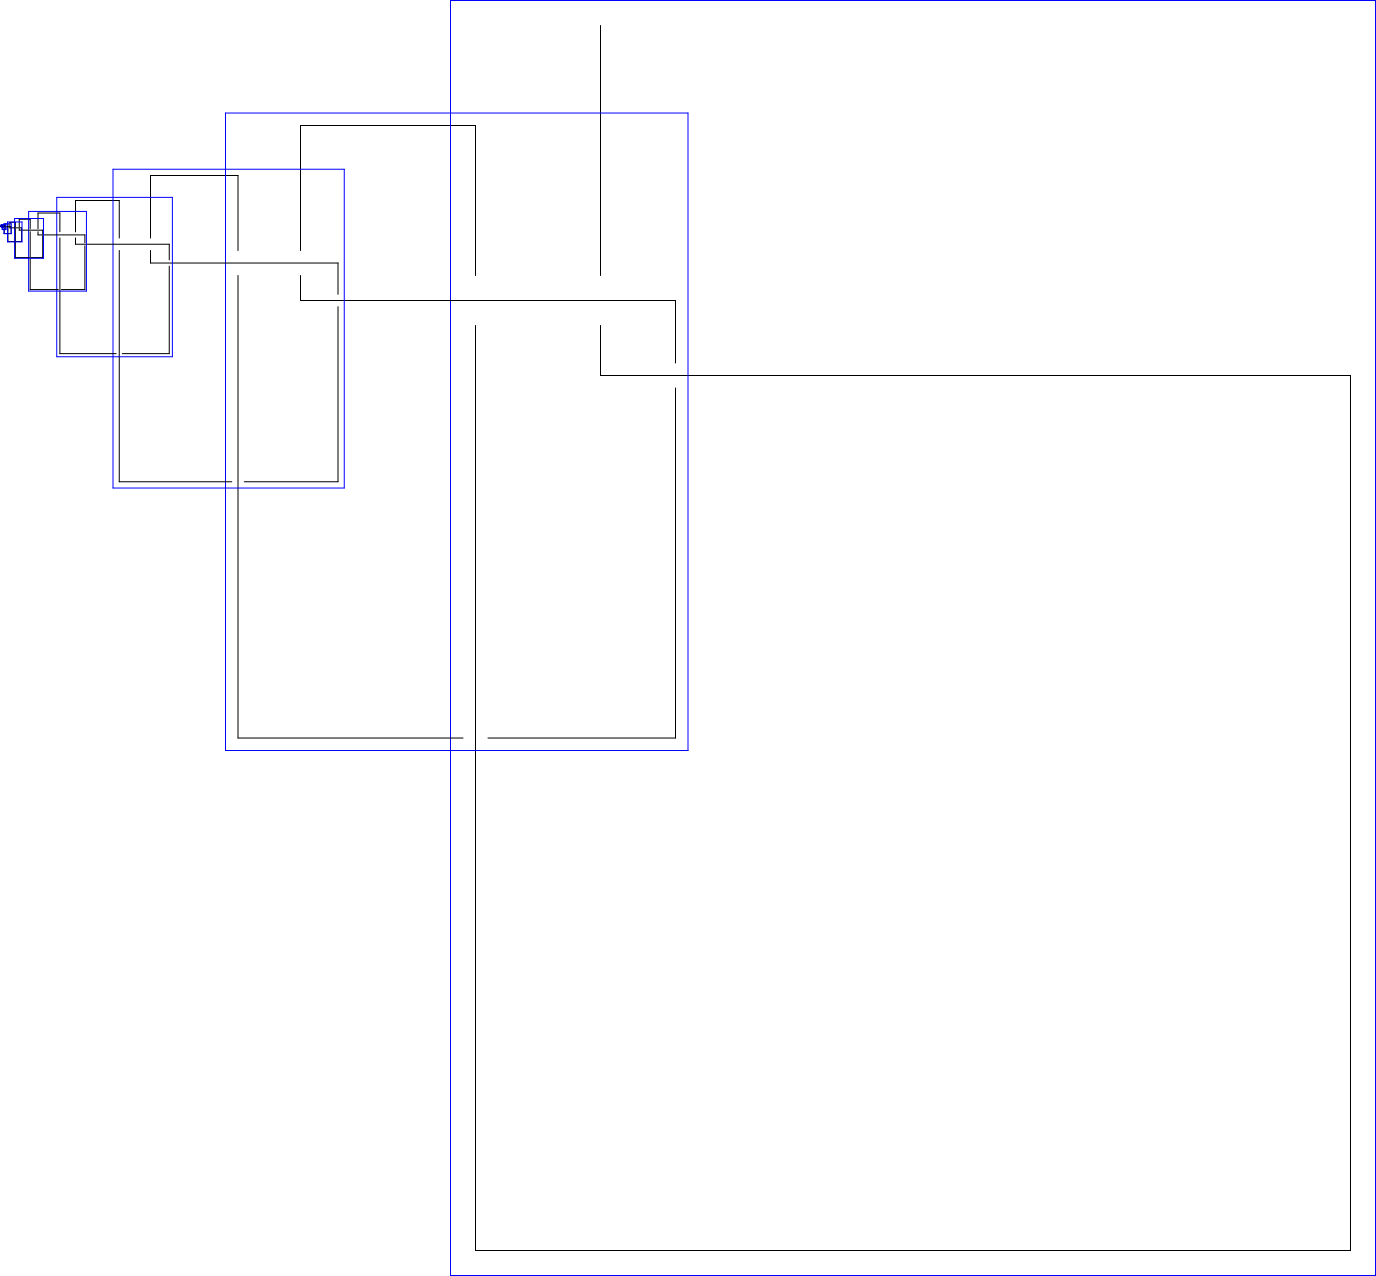
\includegraphics[scale=.2]{figures/preface/loops.pdf}
% \end{figure}


% The idea is to take a
% sequence of nested closed neighborhoods


%  set our attention on
% trying to understand existing literature on wild knots

% This led to a deep dive into the relationships between topological
% knots and their diagrams.

% Hence, phase II of the thesis could be best described as
% \begin{enumerate}[label=(\arabic*)]
%   \item
% \end{enumerate}

% The first plan of attack was to try and find a flaw in the uniform
% convergence argument. One was not immediately obvious to us, although
% this does not mean an error does not exist. Hence, we turned to


% As it turned out, this was also quite ambitious. In the past century
% almost all of the focus of the discipline of Knot Theory has been on
% tame knots. This presents a problem for our purposes,


% Of course, we claim that the example given above \emph{is
%   tame as well} --- the problem is that


% This led to a \emph{deep} foray into the foundations of knot theory,
% to find where the inconsistency lay.

% In particular, our example seemed to suggest an inconsistency between
% (\cref{def:cdef1}) and (\cref{def:cdef2} and \cref{def:cdef3}). To the
% best of our knowledge, this is not actually the case --- rather, the
% confusion seems to arise from hidden hypotheses and/or collisions in
% vocabulary. In \cref{def:cdef1}, we start with an arbitrary embedding
% $K : S^1 \into \RR^3$. In \cref{def:cdef2} and (with some further
% clarifying additions) \cref{def:cdef3}, we're implicitly working in
% the \emph{smooth} category --- meaning we require the knot $K$ to have
% a well-defined tangent vector at every point. This precludes
% embeddings like the one shown in \cref{fig:pref-strange-unknot}; it's
% unclear how to specify a well-defined tangent vector at the limit
% point of the loops.



% The loop nonsense above IS locally flat.

% For S^1 -> R^3, tame implies locally flat
% Hence, not locally flat -> not tame

% Part of the reason this took so long to discover was that as far as we
% can tell, the term \emph{piecewise linear} has been used
% inconsistently in the literature, {\color{green} and (worse still) on
%   StackOverflow!} In particular, sometimes the definition of
% \emph{piecewise-linear} is made in implicit reference to \emph{finite}
% simplicial complexes, and other times, it is made in reference to
% \emph{locally-finite} simplicial complexes.\footnote{If this is a
%   misunderstanding on the author's part, the reader is encouraged to
%   get in contact so that this characterization can be fixed!}


% But actually, the confusion doesn't stop there. As


% This
% led us to take an extended foray into the foundations of knot theory,
% ultimately shifting the focus of the project towards
% \begin{leftbar}
%   ``Seeking a better understanding of the relationships between knots
%   and knot diagrams, with a particular eye towards trying to find an
%   analog of Reidmeister's Theorem for wild knots.''
% \end{leftbar}

% \noindent \textbf{Common Definition 1} (Tame Knot):

% \noindent \textbf{Common Definition 2} (Tame Knot):

% \noindent \textbf{Common Definition 3} (Tame Knot):



%  to carefully examine the foundations of
% knot theory, and try and determine whether Reidemeister's theorem
% could be extended in way to knots with finitely-many wild points.

% \nomenclature{$c$}{Speed of light in a vacuum inertial frame}
% \nomenclature{$h$}{Planck constant}

% \printnomenclature

%%% Local Variables:
%%% TeX-master: "../../kobayashi-thesis"
%%% End:


\mainmatter


\chapter{Introduction}\label{chap:intro}
\setlength\epigraphwidth{.8\textwidth}
\epigraph{The night Max wore his wolf suit and made mischief of one kind\\
  and another\\
  his mother called him ``WILD THING!''\\
  and Max said ``I'LL EAT YOU UP!''\\
  so he was sent to bed without eating anything. }{---Maurice Sendak,
  \emph{Where the Wild Things Are}}

Before we begin: if the reader has not yet read the
\hyperlink{chap:preface}{preface}, we would like to take this
opportunity to mention its existence. Among other things, it contains
a \hyperlink{tab:notation}{table of notation} (\cref{tab:notation})
and a \hyperlink{pref:formatting}{brief note} on the formatting of the
document.

\section{Two Overviews of the Project}\label{sec:two-overviews}
We will give two birds-eye views of some of the questions we've
examined over the course of this project. The first
(\cref{subsec:chronological-overview}) is presented in
\emph{chronological} order, so as to capture more of the overarching
motivation to the topics we pursued. We hope this will help to ground
the reader in a sense of how each component of the project grew out of
the previous ones, and that it can also help orient new researchers
who are investigating similar questions to the ones we pursued. Note,
by virtue of this choice in presentation, it might be harder to get a
sense for ``where things are going'' while reading this section.

To address this, the second (\cref{subsec:more-explicit-description},
\cpageref{subsec:more-explicit-description}) contains more technical
detail, and stays much closer to the final layout of topics within the
document. Essentially, it is meant to function as an annotated table
of contents, listing big takeaways and/or theorems from each section
of the report. It is also much terser than the first, owing to its
different objective.

Naturally there is some redundancy between these two summaries, but we
hope that their different focuses will afford clarity to the reader in
navigating the content. On a final note, we should mention that
careful definitions of all the concepts presented below can be found
later; the ones here are occasionally given in loose terms to help
keep the pacing brisk.


\section{A Chronological Overview}\label{subsec:chronological-overview}

At the outset, our goals were as follows.
\begin{enumerate}[label=(\arabic*)]
  \item Give clear/engaging exposition on the foundations of knot
    theory, paying close attention to rigor.
  \item Explore the extent to which unknotting moves give us way to
    define new algebraic structure on the category of knots. In
    particular, we were interested in the loosely ``multiplicative''
    structure of the connected sum, and wanted to see if we could find
    an underlying ``addition'' operation corresponding to it.
\end{enumerate}
We leave it to the reader to judge our handiwork regarding (1).
Regarding (2), after a semester of largely-fruitless exploratory work,
it became clear that this was too ambitious for a 1-year
project.\footnote{That's not to say we did nothing --- we have some
  interesting exploratory results, but most of them are computational,
  as working theoretically turned out to hinge on the following
  example (which led us down the bottomless rabbit hole of \emph{wild
    knot theory}).}

However, there was at least one intriguing result that came out of our
attacks. In attempting to define all modifications of the Gauss code
in terms of group actions, we needed a way to treat all knots as if
they contained the same number of crossings. Essentially, this was
because we needed a way to interpret what ``flip crossing 17'' would
mean if we only had a 3-crossing knot. This led us to the following
example of a knot that \emph{appears} to be ambient-isotopic to the
unknot, despite having infinitely-many crossings (shown in
\cref{fig:pref-strange-unknot}).
\begin{figure}[H]
  \centering
  \includegraphics[width=.6\linewidth]{figures/rectifiable-knots/winf.pdf}
  \caption{A strange unknot\ldots}
  \label{fig:pref-strange-unknot}
\end{figure}
We'll show this is a valid embedding of $S^1$ when we talk about it in
depth in \cref{sec:countable-r1-moves-for-sn}.\footnote{In particular,
  see \cref{thm:countable-gluing-ambient-isotopies}} Note, the proof
we will give in that section differs from the sketch we're about to
describe; the latter came first chronologically (and ends up being a
bit more powerful), but is messier to work with.

Anyways: The loose idea is that we can create a uniformly convergent
sequence of ambient isotopies yielding \cref{fig:pref-strange-unknot}
in the limit. We can show that the associated homeomorphisms are
uniformly convergent, and that their inverses are as well. Then, after
arguing bijectivity, we can apply the fact that a uniform limit of
continuous functions is continuous to get a homeomorphism in the
limit. Finally, we apply a uniform convergence argument to the overall
ambient isotopy to show it is continuous.

% The loose idea is
% that we can realize \cref{fig:pref-strange-unknot} by looking at a
% countable sequence of ambient isotopies that act on disjoint sets of
% decaying diameter. Because the sets are all disjoint, we don't lose
% bijectivity in the limit, and because the diameters decay, we can
% argue continuity is preserved as well.\footnote{This is actually not
%   our original method of proof,


% }

%   In any case: later, we pursue a similar result, but drop the
%   assumption of \emph{disjointess} and instead apply uniform
%   convergence (see \cref{prop:uniform-convergence}, in particular
%   \cref{thm:uniformly-convergent-ambient-isotopy}). It will be
%   \hypertarget{important-note-on-method}{\textbf{very important}} to
%   be careful in this approach, as there are some very-similar
%   looking knots where this strategy doesn't work (see
%   \cref{ex:fox-artin-curve}). In particular, without the
%   disjointness condition, sometimes we can lose bijectivity in the
%   limit in ways that are not obvious.



This example was particularly puzzling, as it seemed to create
inconsistencies in the common definitions of \emph{tame knots}, a
handful of which are given below:
\begin{commondef}\label{def:cdef1}
  We say a knot $K : S^1 \into \RR^3$ is \emph{tame} iff it is ambient
  isotopic to a polygonal knot.
\end{commondef}
\begin{commondef}\label{def:cdef2}
  We say a knot $K : S^1 \into \RR^3$ is \emph{tame} iff for every
  point $x$ on $K$, there exists a neighborhood $U_x$ such that the
  pair $(U_x, K \cap U_x) \cong $ the standard $(\mrm{ball},
  \mrm{diameter})$ pair.
\end{commondef}
\begin{commondef}\label{def:cdef3}
  We say a knot $K : S^1 \into \RR^3$ is \emph{tame} iff it can be
  thickened to an embedding of a solid torus.
\end{commondef}
\begin{commondef}\label{def:cdef4}
  We say a knot $K : S^1 \into \RR^3$ is \emph{tame} iff it has
  finitely many crossings.
\end{commondef}
In particular: we were claiming that our $K$ satisfied
\cref{def:cdef1} (which would also imply satisfying \cref{def:cdef2}),
but it was in no way obvious that it satisfied \cref{def:cdef3}.
Further, \cref{def:cdef4} seemed to be outright violated. Hence the
project shifted focus to examining the foundations of Knot Theory in
an attempt to verify
\begin{enumerate}
  \item Whether or not any inconsistency was actually present, and
  \item If so, where? If not, why didn't we think so?
\end{enumerate}
For (a), the first plan of attack was to try and determine whether
there was a flaw in our theorems. One was not forthcoming to
us.\footnote{Of course, this does not mean an error does not exist
  (the reader is encouraged to get in touch if the find a problem),
  but we are fairly confident in our techniques, especially given that
  we provided multiple approaches (E.g.,
  \cref{thm:countable-gluing-ambient-isotopies},
  \cref{sec:c1-countable-r1}).}

Having failed to find an error in our proofs (but being convinced at
the time that a flaw must exist), we set about trying to disprove our
claim by finding another context where the same technique yielded a
contradiction. This led us to the following example of
\cite{FoxArtin}, here drawn as an arc\footnote{An \emph{arc} is an
  embedding of $[0,1] \into \RR^3$ (as opposed to a knot, which is an
  embedding of $S^1 \into \RR^3$).} made of countably-many line
segments (\cref{fig:fox-artin-ce})
\begin{figure}[H]
  \centering
  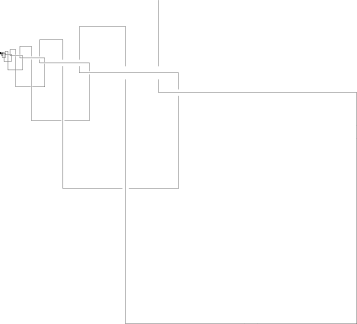
\includegraphics[scale=.19]{figures/preface/loops-no-boxes.pdf}
  \caption{The Wild Arc of Fox-Artin}
  \label{fig:fox-artin-ce}
\end{figure}
Interestingly, although it's possible to use Reidemeister II moves to
undo any finite number of the ``stitches'' in the above, this knot is
provably \emph{inequivalent} to any tame knot. To show this, Fox and
Artin developed an invariant for ``tameness'' based on the fundamental
group of a nested sequence of closed neighborhoods of the wild
point.\footnote{We reproduce their argument in
  \cref{ex:fox-artin-curve}.} The idea is that by showing that the
induced homomorphisms at each step are necessarily nontrivial, one can
show no ambient isotopy to a tame arc exists.

At this point, we took a deep dive into investigating the question of
when two \emph{arbitrary} knots are ambient-isotopic. In particular,
we wanted to know when we could use countable sequences of
Reidemeister moves. This became the focus of most the remainder of the
project.

As it turns out, this was far harder than we suspected. In fact,
across multiple books, papers, and conversations with knot theorists,
we heard sentiments like the following:
\begin{itemize}
  \item ``It would be fair to say that we know next to nothing about wild
    knots. Hence, we will not discuss them. We leave the problem to
    future generations.'' -An unnamed book
  \item ``I feel like I really know nothing about wild knots\ldots and
    I think most knot theorists would say the same (about themselves
    as well as me).'' -An unnamed knot theorist
  % \item ``If a wild knot embeds in $\RR^3$ and nobody cares, does it
  %   really exist?'' -Another mathematician
\end{itemize}
And so on. Further, a book we just recently discovered that treats the
general topic of embeddings of manifolds (\cite{Daverman}) has this to
say about the requirements for approaching the topic:
\begin{leftbar}
  ``What background is needed for reading this text? Chiefly, a
  knowledge of piecewise linear topology. [Although] to be honest, [we
  must also] presume extensive understanding of both general and
  algebraic topology [\ldots] as well. In an attempt to limit our
  presumptions, we [\ldots] shall take as granted the results from two
  fairly standard texts on general and algebraic topology [\ldots]
  each of which can be treated quite effectively in a year-long
  graduate course. Unfortunately, even [these] turn out to be
  insufficient for all our needs.''
\end{leftbar}
Naturally, all of this would be sure to strike fear into the heart of
any undergraduate attempting to tackle the problem, particularly one
who has yet to actually complete a single formal course in Topology.
Thus, it is a good thing we did not discover these problems until near
the completion of the project.

% {\color{blue} this isn't exactly true. I knew we didn't know a lot
% about wild knots, I just didn't
% know \emph{how much} we didn't know.}

% It gets worse. There \emph{is} a nice text that we just stumbled
% across while assembling our

% However, it turns out this does not actually provide us with a
% counterexample for our technique. After a lot of head-scratching, we
% discovered that there were some hidden problems in the Fox-Artin
% curve. The one we highlight here is that we lose bijectivity in the
% limit (we illustrate this in
% \cref{fig:fox-artin-pulling-out-a-stitch}), but it's worth noting that
% we also only get uniform convergence in the forward direction of our
% homeomorphism. Anyways, the point is that the problem was that the
% hypotheses of our theorems were not satisfied; the argument itself
% still seemed to hold.

Being blithely unaware of the dangers ahead, we forged dutifully
onward. Due to some confusion with the definition of a locally-finite
simplicial complex, we ended up focusing a large amount of our effort
on studying the question of which knots can be converted (through
ambient isotopy) to a countable union of polygonal segments. The
source of the confusion was as follows: If one ignores the weak
topology\footnote{Or, in our case, (a) simply does not know about its
  existence, followed in short time by (b) even upon learning about
  its existence, does not understand its significance} and views
simplicial complexes solely in terms of partitioning $\RR^n$, then it
becomes possible to find ``locally-finite'' ``simplicial complexes''
realizing many wild knots as chains of 1-simplices (with the wild
points being included as separate $0$-simplices). The prototypical
example is to do something like the following:
\begin{leftbar}
  For all $n \in \NN$, let $a_n = \set{\frac{1}{n+1}}$, $b_n =
  \set{\frac{1}{n}}$, and $I_n = \bk{\frac{1}{n+1}, \frac{1}{n}}$.
  Also let $I_\infty = \set{0}$. Then
  \[
    K = \set{I_\infty} \cup \bigcup_{n \in \NN} \set{a_n, b_n, I_n}
  \]
  satisfies the following properties:
  \begin{enumerate}
    \item For all $\sigma \in K$, every face $\tau$ of $\sigma$ is
      also an element of $K$
    \item For all $\sigma_0, \sigma_1 \in K$, if $\sigma_0 \cap
      \sigma_1 \neq \varnothing$, then $\tau = \sigma_0 \cap \sigma_1$
      is a sub-face of both $\sigma_0$ and $\sigma_1$, and
    \item For all $0$-simplices $\sigma \in K$, $\sigma$ is a vertex
      of at most finitely-many simplices in $K$.
  \end{enumerate}
\end{leftbar}
At first glance, one might protest that $I_\infty$ should really be a
face of \emph{infinitely-many} of the $1$-simplices. Morally, maybe
yes. But definitionally, no, this is actually not the case. $I_\infty$
is only incident in one simplex, namely itself. Indeed, one can see
that for all $n \in \NN$, $I_n \cap I_\infty = a_n \cap I_\infty = b_n
\cap I_\infty = \varnothing$. We can create analogues in higher
dimensions; E.g., an $\RR^2$ example is given by the following.
\begin{figure}[H]
  \centering
  \includegraphics[scale=.5]{figures/wild/simp-comp-down.pdf}
  \caption{A ``locally-finite'' simplicial complex.}
\end{figure}
With this as motivation, we built up some formal machinery for working
directly with diagrams of wild knots provided that the crossing points
remain transverse and discrete.\footnote{For those familiar with the
  subject matter, this relaxes our axioms for ``regular diagrams'' to
  allow possibly \emph{countably} many crossings.} This allowed us to
show in \cref{thm:discrete-diagram-countably-polygonal} that
\emph{all} such knots are ambient isotopic to representatives
comprised of a countable union of polygonal segments. This was very
exciting, since it seemed it could open the door to attempting to
generalize Reidemeister's theorem to countable sequences of moves. We
already had an \emph{if} direction from
\cref{thm:uniformly-convergent-ambient-isotopy}; we were interested in
an \emph{only if}. Unfortunately, we did not have time to see it
through. This would be an interesting direction for future work.

Having taken a deep foray into the topic of wild embeddings \& built
up more machinery, at long last we returned back to our countable
Reidemeister I example, now much more confident in its correctness.
Using it as the cornerstone, we built up some basic definitions for
our desired algebraic framework (\cref{sec:defining-the-action}), and
created some basic tools for performing computational
search.\footnote{The code is available on Github:
  \url{https://github.com/redpanda1234/permutation-knots}}

We should emphasize that the primary strengths of this new formalism
do not stem from it delivering us a new understanding of the
equivalence problem (although its possible that connections will arise
in the future), but rather from the fact that it seems to offer a
natural language for studying unknotting moves. We would be very
interested in seeing future work in this direction.

This more-or-less wraps up the timeline for the project. In composing
this report, we were given an opportunity to reflect on what the
``heart'' of the project was. From the above, it might seem like an
answer is hard to glean, given the wide range of tangents we embarked
on. We would agree. In fact, we think that in it's own way, the
\np{``slipperiness'' of identifying the correct road forward in
  absence of established machinery} was the defining feature of our
work. We found that often, as soon as we stepped outside the scope of
Reidemeister's theorem, the standard intuition we used to approach
knot theory was fundamentally challenged at every turn. There were
many theorems we took for granted --- e.g., ``ambient isotopy and
ambient orientation-preserving homeomorphism are equivalent'' --- that
turned out to contain hidden PL hypotheses that we did not quite
understand the significance of. % Untangling this web of dependencies
% was the source of great confusion, but we.

Thus, in choosing how to present our findings, we decided to strive
for being as encyclopedic as possible, to help orient those interested
in future work. To that end we have placed particular attention on (a)
pointing out ways in which this perspective might be useful in
studying tame embeddings, (b) drawing attention to important
counterexamples that challenge our intuition, and (c) striving to be
maximally rigorous in working with our proofs.

% {\color{blue}
We hope they find the reader well.
% }

\section{The More Technical
  Overview}\label{subsec:more-explicit-description}
The document is structured as follows.
\begin{enumerate}[label=(\Roman*)]
  \item \cref{chap:intro}: In this chapter (which you are reading
    right now), we give two high-level overviews of the project,
    including one that has a more personal/chronological feel to it
    (\cref{subsec:chronological-overview}), as well as a more detailed
    ``table of contents,'' which includes, among other things, a
    recursive reference to its own contents
    (\cref{subsec:more-explicit-description}).
  \item \cref{part:fundamentals}: Fundamentals of Knot Theory. Here,
    we give an overview of the big picture ideas in knot theory, and
    list some basic definitions. We encourage those more familiar with
    the topics to read \cref{chap:motivation} but skip the rest.
    \begin{enumerate}[label=\arabic*)]
      \item In \cref{chap:motivation}, we discuss the knot equivalence
        problem, with particular focus on an analogy with determining
        equivalence of arithmetic expressions. We discuss the
        differences between these two contexts (e.g., the absence of a
        good simplification algorithm for knots), as well as what
        kinds of additional structure on the knot category might help
        get around some of these difficulties in the future. This
        serves to motivate the approach taken in
        \cref{chap:connections-to-sn}
      \item In \cref{chap:knots-and-knot-diagrams}, we provide the
        standard definitions for knots, ambient isotopy (highlighting the
        problems with choosing something like \emph{isotopy} instead
        as our definition of equivalence), tameness, regular diagrams,
        orientation, and so on. This is targeted mainly at those who
        are new to the topic; experts will probably find nothing
        surprising. One thing of note is that we place emphasis on
        highlighting the fact that going from ``working with knots''
        to ``working with knot diagrams'' should not be taken for
        granted.
    \end{enumerate}
  \item
    \cref{part:unknotting-moves-and-combinatorial-representations}:
    Combinatorial Representations. Here, we discuss what we call
    \emph{combinatorial representations}, i.e.\ ways of abstracting
    information in knot diagrams to strings that can be manipulated
    purely algebraically / combinatorially.%  The overarching desire is
    % to
    % to find a nice rule-based framework
    % Our prototypical (and in
    % fact, only) example is the signed Gauss code. We discuss
    \begin{enumerate}[label=\arabic*)]
        \setcounter{enumii}{3}
      \item In \cref{chap:gauss-code}, we introduce the signed Gauss
        code for a knot diagram. We discuss the Gauss code encoding of
        Reidemeister moves, especially the planarity constraint of
        Reidemeister II. A significant portion of the exposition is
        dedicated to discussing what we have called the \emph{diagram
        graph} (\cref{def:diagram-graph}), which is a graph
        constructed from the Gauss code that is particularly natural
        for computational manipulation. In particular, we prove that
        it has a unique planar embedding, and thus can be used to
        verify proposed Reidemeister II moves (we give a sketch for a
        greedy algorithm performing this check).

        Finally, we finish by introducing virtual knots as a way to
        avoid the planarity concerns of Reidemeister II, and work
        instead in a more purely combinatorial context. Discussion of
        the forbidden moves leads us to \emph{briefly} mentioning
        unknotting moves, and the intriguing sense in which they
        encode ``recipes'' for how to build knots from the unknot.
      \item In \cref{chap:connections-to-sn}, motivated by the
        discussion of unknotting moves, we build up basic definitions
        for our formalism that connects Gauss codes to actions of the
        symmetric group on a countable set. The desire here is to
        flesh out the idea of unknotting moves as ``building'' knots
        and ``converting them into each other.'' Unfortunately, it
        seems like on a purely theoretical level, it's not possible
        to reconcile knot equivalence with the group structure in a
        sensible way. Nonetheless, we did see some unexpected patterns
        in performing computer searches with \texttt{sage}.

        Underpinning all of our results in this chapter is the example
        of an unknot with a countable number of crossings. To show
        this is valid, we use a slightly simpler version of the
        uniform convergence proof we give later
        (\cref{thm:uniformly-convergent-ambient-isotopy}). To be extra
        sure that the result is valid (even if our proof turns out to
        secretly contain a flaw), we construct a $C^1$ embedding for
        our example of interest (\cref{sec:c1-countable-r1}),
        which suffices to guarantee it is tame (see
        \cref{chap:feral-gallery}).
        % In terms of a purely theoretical approach, it seems very
        % challenging to
        % Indeed, although we do not explicitly discuss this, one can
        % view unknotting moves as families of elements that
        % ``complete'' the Reidemeister moves in the sense of making
        % them sufficient to generate the entire group.
    \end{enumerate}
  \item In \cref{part:wild-knots}, we shift our focus to general
    topological embeddings, withe the goal of getting a better
    understanding our examples of countable Reidemeister I moves.
    \begin{enumerate}[label=\arabic*)]
        \setcounter{enumii}{5}
      \item In \cref{chap:tame-and-wild-knots}, we clarify common
        definitions for tameness and wildness that we have found in
        the literature, reconciling those that we can with the terms
        used when studying more general embeddings of $m$-manifolds
        into $n$-manifolds. We try to be particularly cognizant of
        which category we are working in at all times.
      \item In \cref{chap:machinery}, we begin building up machinery
        for our later work in studying ambient isotopy for general
        topological embeddings. We develop two tools (strand
        separation and uniform converence) which prove useful for
        working with wild knots whose wild points are topologically
        discrete. We do not build machinery for working with
        everywhere-wild knots.
      \item In \cref{chap:ambient-isotopy-in-r2}, we apply these tools
        in the case of $\RR^2$, and show that all curves $K : S^1
        \into \RR^2$ are ambient isotopic (this will be important when
        we move to $\RR^3$ in \cref{chap:moving-into-r3}). In
        \cref{sec:feral-points}, we discuss the pathologies that can
        arise in diagrams in $\RR^2$, which we refer as \emph{feral}
        behavior.
      \item In \cref{chap:moving-into-r3}, we use the techniques of
        \cref{chap:machinery} and \cref{chap:ambient-isotopy-in-r2} to
        study ambient isotopies in $\RR^3$. The loose idea is that as
        long as the crossing points in our diagrams are toplogically
        discrete, we have a bunch of strands that essentially act like
        they're curves embedded in $\RR^2$ (because, after all, they
        don't cross). This reduces the behavior to results covered by
        \cref{chap:ambient-isotopy-in-r2}. By then showing we can also
        constrain the behavior of our embeddings \emph{near} crossing
        points, we can then show that if a wild knot has a diagram
        with topologically discrete crossings, then it is ambient
        isotopic to a representative comprised of a countable union of
        polygonal segments. We conclude with some directions for
        future work, and offer a very brief sketch of how one might
        build an analogue to Reidemeister's theorem in this context.
      \item Lastly, in \cref{chap:summary}, we summarize the results
        of the project, and discuss possible ways of turning our
        ``crossing-discrete wild knots'' into a category more directly
        analogous to the PL case. This concludes the main body of the
        document.
    \end{enumerate}
  \item \cref{part:appendix} is the appendix. Here, we include some
    miscellany that didn't fit particularly well into any parts of the
    main document.
    \begin{enumerate}
      \item[A)] \cref{chap:feral-gallery} contains two extra feral
        knots that we have parameterized by a $C^1$ embedding.
      \item[B)] \cref{appendix:pl-topology} contains a basic
        crash-course in PL Topology, with an emphasis on the ``crash''
        part.
      \item[C)] \cref{chap:misc} includes misc.\ data from the
        project. This includes tables for the cycle representations
        computed in \cref{chap:connections-to-sn}.
    \end{enumerate}
\end{enumerate}


% The following gives





















% Anyways: As discussed in the preface, the original goals of the thesis
% were (1) to give lucid exposition on the fundamentals of knot theory,
% and (2) to study unknotting moves and how they might offer more
% explicit algebraic structure for knots.

% Regarding (1), we've sought to place particular emphasis on two
% points:
% \begin{enumerate}[label=\roman*)]
%   \item The material should be accessible to readers who don't
%     yet have extensive background in the field. Importantly,
%     ``accessible'' here does not mean eschewing rigor, but rather
%     taking care to motivate it properly.%  Instead, we
%     % have attempted to offer intuition for every definition given, as
%     % well as counterexamples illustrating why these particular
%     % definitions are ``the right ones.''
%   \item The exposition should try and communicate just as much
%     \emph{excitement} as it does technical content.
% % In addition to communicating understanding of the material,
% %     the exposition should give a sense for what makes the subject
% %     interesting. The hope is that the reader
% \end{enumerate}
% In short, the goal is to equip the reader with knowledge and convince
% them to explore further on their own. We chose to focus on a concept
% that we would personally have benefited from seeing emphasized early
% on in our investigation of knot theory; namely, the distinction
% between \emph{knots} and \emph{knot diagrams}. This topic is of
% central importance later on in the document, so we think focusing on
% it here is appropriate. In our descriptions, emphasis is placed on the
% use of pictures, as well as analogies with other mathematical
% concepts.

% Regarding (2): As we discovered, this goal was a bit too ambitious to
% take on during our limited timeframe. However, we still believe it
% represents a promising direction for future work, and hence have
% included some discussion of our motivation as well as some of our
% exploratory work.

% The main idea is to consider virtual knots as equivalence classes of
% elements of the finitary symmetric group on a countable
% set.\footnote{Of course, the equivalence relation is prohibitively
%   expensive to compute (since otherwise we'd have an efficient
%   solution to the knot equivalence problem).
%   % but the representation
%   % has the interesting property of giving us a new notion of ``knot
%   % multiplication.''
% } The correspondence is established in such a way that the Gauss code
% can be understood as an action of these permutations on a standard
% infinite sequence of string characters, by identifying the portions of
% the sequence that have been deranged from standard position. One
% interesting side-effect of this encoding is we can now define a new
% group-like operation on knots, namely composing the representing
% permutations. When we do so, we see that the action of these ``product
% knots'' on the standard sequence often yields Gauss codes that
% represent link diagrams.\footnote{In fact, simply looking at the
%   number of components in these link diagrams (not even their
%   connectivity) distinguished all but a handful of knots up to $8$
%   crossings. However, this could be a superficial result since we made
%   no attempts to examine ways of normalizing the effects of
%   Reidemeister moves, so this is not even an invariant.} We would be
% curious to see whether this provides a new interpretation for bracket
% polynomials, such as those in our previous work
% (\cite{Kobayashi2019Sep}).
% % 'll see that there are some connections between
% % \np{algebraic properties of knots} and \np{permutation groups}.
% % {\color{pink} This will come in the form of some sort of isomorphism.}
% % Tame knots can be thought of in terms of the \emph{finitary symmetric
% %   group} (all finite permutations on $\NN$), while wild knots whose
% % \np{sets of wild points are topologically discrete} can be understood
% % as arbitrary elements of $\ms S_{\NN}$. We have not investigated
% % similar ideas for knots that are everywhere-wild.}

% In establishing the connection described above, we'll see that it's
% important to come up with a diagramming system that gives every tame
% knot the same ``number'' of crossings. This is where the example of
% the unknot with countable Reidemeister I moves (see
% \cref{fig:pref-strange-unknot}, \cpageref{fig:pref-strange-unknot})
% comes into play. This (and similar examples) will comprise the
% remainder of the document, which represents a third goal on the list:
% \begin{enumerate}
%   \item[(3)] Gain a better understanding of wild knots.
% \end{enumerate}
% In this direction, first we will provide explanations of how our
% example can be reconciled with some of our intuitive definitions of
% what it means for a knot to be ``tame.'' In particular, we will
% construct an ambient isotopy to a \emph{PL knot}, show that there
% exists a \emph{smooth} knots realizing diagrams like
% \cref{fig:pref-strange-unknot}, and give a sketch for how we can
% construct a lift from this countable Reidemeister I knot to an
% embedding of the solid torus $S^1 \times \mathbb{D}^2$.

% This led us to some further investigations of wild knots. To finish up
% the project, we prove a coarse sort of hierarchical result regarding
% the ``wildness'' of knots (again, using the invariant of
% \cite{FoxArtin}), and also develop a sketch of how to generalize
% Reidemeister's Theorem using arguments based on uniform continuity and
% / or uniform convergence.

% These three goals are each contained in a separate Part of the
% document. \cref{part:fundamentals} contains our exposition on the
% fundamentals of knot theory, \cref{part:unknotting-moves} contains our
% exploration of unknotting moves and combinatorial structures, and
% \cref{part:wild-knots} discusses the countable Reidemeister I moves in
% more detail, and also examines some aspects of the ambient isotopy
% problem for wild knots.

%%% Local Variables:
%%% TeX-master: "../../kobayashi-thesis"
%%% End:


\part{Fundamentals of Knot Theory}\label{part:fundamentals}
\chapter{Motivation}\label{chap:motivation}
\setlength\epigraphwidth{.6\textwidth}
\epigraph{That very night in Max's room a forest grew\\
and grew--\\
and grew until his ceiling hung with vines\\
and the walls became the world all around}{---Maurice Sendak,
\emph{Where the Wild Things Are}}


One of the most fascinating things about knot theory is the disconnect
between the relative ease of posing a question and the great
difficulty of providing a rigorous answer to it. Granted, many
mathematical fields are like this --- but knot theory is somewhat
curious in the \emph{extremity} of the mismatch. Many of the most
fundamental problems in the field can be boiled down to ideas that are
accessible to any lay-person, and yet are quite challenging to
approach mathematically.

Understanding \emph{why} is the goal of this chapter of the document.
As a motivating example, we discuss the problem of \emph{knot
  equality} through analogy with equality of arithmetic strings. This
analogy ends up also serving as the motivation for our proposal that
studying \emph{unknotting moves} could offer new insights into the
structure of the knot category.

In \cref{chap:knots-and-knot-diagrams}, we give background
definitions, with a focus on emphasizing the fact that relationships
between \emph{knots} and \emph{knot diagrams} are subtle, and should
not be taken for granted. As we will see later on, loosening what we
call ``an admissible diagram'' can give us some valuable tools for
understanding Knots.

Lastly, in \cref{sec:polygonal-knots} we offer a brief discussion of
polygonal knots. Mainly, this is a gallery of some pictures; rigorous
treatment is left to the section in the appendix about PL Topology and
our examination of tameness in \cref{part:wild-knots}.
% {\color{red}
%   elongate this} before launching into our new results, given in
% \cref{part:unknotting-moves} and \cref{part:wild-knots}
% .



The remainder of the discussion in this chapter is presented at a high
level, with just a few (optional) formal definitions.\footnote{We hope
  the more rigor-oriented readers will be patient in tolerating some
  imprecision for the time being, but if not, formal definitions can
  be found in \cref{chap:knots-and-knot-diagrams},
  \cpageref{chap:knots-and-knot-diagrams}.} We hope the ideas remain
both \np{accessible to a non-technical audience} and \np{interesting
  for experts}.
% Before leaping straight into the technical details of the project, I
% want to be sure to establish a strong sense of what makes this project
% interesting, and why we might think of it as a particularly natural
% way to better understand algebraic structure in knots. First, let's
% actually define some terms.
\section{The Big Picture}
\begin{figure}[H]
  \centering
  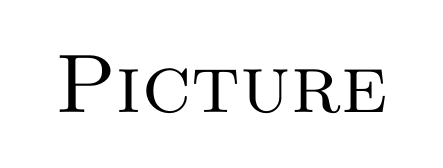
\begin{tikzpicture}[every node/.style={scale=3}]
    \node () at (0,0) {\scshape Picture};
  \end{tikzpicture}
  \caption{A Bad Joke}
\end{figure}
In mathematics, a \emph{knot} is an embedding of a circle into another
space.\footnote{In loose terms, ``embedding'' means that (a) if we
  zoom in closely enough to our knot, it looks like a line, and (b) if
  we walk all the way around in one direction, we get back to where we
  started. This is made formal in \cref{sec:KnotDef}.} Intuitively,
think of taking a rope and twisting it around in space in all sorts of
ways, finally fusing the ends together so that we get a closed loop:
\begin{figure}[H]
  \centering
  \includegraphics{figures/intro/knotcons.pdf}
  \caption{Constructing a knot}
  \label{fig:knotcons}
\end{figure}
Note, our loop does not need to have any twists to be considered a
knot --- a regular old circle is a perfectly valid knot! We call this
the \emph{unknot}, and we'll see that it has some interesting
properties later (e.g., it acts like the number $0$ for a knot
``addition'' operation).

We say two knots $K_1$, $K_2$ are \emph{equivalent} (denoted $K_1
\cong K_2$) if we can deform $K_1$ into $K_2$ without cutting the rope
and gluing it back together. For example, the left two knots in the
diagram below are equivalent, and both are distinct from the knot on
the right.\footnote{At this point, it is worth noting that there's a
  technical distinction between a \emph{diagram} for a knot and the
  actual knot itself. We'll return to this later when we define things
  rigorously, but gist is that knots live in $\RR^3$ and diagrams are
  projections onto $\RR^2$.}
\begin{figure}[H]
  \centering
  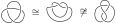
\includegraphics[width=.5\linewidth]{figures/intro/three-knots.pdf}
  \caption{Two equivalent knots and one inequivalent one}
\end{figure}
One of the central questions in knot theory is ``given diagrams $D_1$
and $D_2$ how do we determine whether they represent the same knot?''
If starting from first principles, this question is \textbf{HARD} to
approach mathematically; in fact it requires a bit of topological
knowledge to even formulate the question properly. Thankfully, in
practice we don't usually need to think about any of that because of a
theorem proven by \cite{Reidemeister1927Dec} and, independently,
\cite{Alexander1926}. In essence, they were able to show that two
``well-behaved'' diagrams\footnote{Again, we'll discuss what
  ``well-behaved'' means in great detail during
  \cref{chap:knots-and-knot-diagrams}, but it boils down to ``the
  string only crosses itself in an $X$ shape.''} $D_1, D_2$ represent
the same knot iff $D_1$ can be turned into $D_2$ by a sequence of the
following so-called \emph{Reidemeister moves:}
\begin{figure}[H]
  \centering
  \includegraphics[width=12cm]{figures/intro/rmoves.pdf}
\end{figure}
\noindent%
which are creatively referred to (in left-to-right order) as
``Reidemeister I,'' ``Reidemeister II,'' and ``Reidemeister III,''
respectively.\footnote{We also include another move, which allows us
  to bend the string arbitrarily as long as we don't introduce a
  crossing.} Note, while Reidemeister III might look complicated, it's
really just saying that we can move one strand between the crossing
formed by two other strands.

On a theoretical level, this is a very elegant characterization of
knot equivalence. However, in practice, determining equivalence is
still quite challenging. Even if $D_1$, $D_2$ are relatively simple
and both represent the same knot, the sequence of moves relating the
two can be quite long. It's even worse when $K_1 \not \cong K_2$,
because then we have to prove a negative result: namely, that there
\emph{does not exist} a sequence of Reidemeister moves takes $D_1$ to
$D_2$! Again, this is usually quite hard. Though Algorithms deciding
the problem do exist, they are currently far too inefficient to be
practical. For those who are familiar with Complexity Theory: It has
been proven (\cite{Hass1998Jul}) that a special case of knot equality
is at least NP. Reidemeister-based algorithms for the general problem
have runtimes like $O(k\uparrow\uparrow n)$ (\cite{Lackenby2016Apr}),
which makes even an NP solution seem out of reach for now.

% and current theoretical results {\color{red} IS THIS
%   TRUE? {\color{orange} put our best bound at EXPSPACE.}}


% It's a little baffling that these seemingly simple objects

But why? This seems like it should be easy! Our objects are very
tangible, the space we're working in ($\RR^3$) is well-behaved, and we
aren't asking for anything too fancy --- just a simple way to
determine equality. How can we understand the source of this
difficulty? Here, an analogy with something more familiar will be
helpful.






% ------------------------------------------------------------------ %
%                                                                    %
%                                2                                   %
%                                                                    %
% ------------------------------------------------------------------ %

\section{An Analogy}\label{sec:an-analogy}
Let's say I hand you two integers $n, m$. Would you be able to tell me
if $n = m$? Most likely the answer is yes. For instance, if I said
\begin{align*}
  n &= 8 & m &= 31
\end{align*}
you'd probably be able to distinguish $n$ and $m$. In particular,
they're uh\ldots not\ldots the same number.

But now let's frame the same problem in a slightly different way.
Suppose I had given you something like
\begin{align*}
  n &= ((1 + 3) + 3) + 1
  & m &= (((3 \cdot 3) \cdot 3) + (2 \cdot 2)) \cdot 1
\end{align*}
instead. Could you still determine if $n = m$? Maybe mental arithmetic
isn't your forte, but in theory the answer is ``yes'' --- these
equations give us the same solutions for $n,m$ as before, we just have
to do a little bit of extra work to see it.
% since the answers are obfuscated by a layer of arithmetic.
\begin{align*}
  n
  &= (4 + 3) + 1
  &
    m
  &= ((9 \cdot 3) + (2 \cdot 2)) \cdot 1 \\
  &= 7 + 1
  &
    m
  &= (27 + (2 \cdot 2)) \cdot 1 \\
  &= 8
  &
    m
    &= (27 + 4) \cdot 1
\end{align*}
For all intents and purposes these are cosmetic differences; they
don't make the problem too much harder to solve than it was before. We
can just simplify the expressions, see that the left gives $8$ and the
right gives $31$, and then we know $8 \neq 31$ so we can go on our
way.

This continues to hold even when the expressions get comically large,
e.g.
{\footnotesize
\begin{align*}
  n
  &= 2\cdot (2\cdot (8 \cdot  (21 - 38) - 7\cdot 6) + (4\cdot (21 +
    (-10 \cdot  (2 - 4))) + 7\cdot 28)) \\
  m &= (2\cdot(-3 \cdot (1500)) - 4) - (4\cdot(18-(8\cdot(10 - (3 -
      12)))))\cdot 15 + 5 \cdot(25\cdot(3\cdot4) - 101)
\end{align*}}
While simplifying these by hand might be tedious and unpleasant, it's
certainly something we could get a computer to do. In fact, programs
for this task are fairly efficient, being able to handle expressions
far larger than the above with near-instantaneous results.\footnote{To
  be precise: We claim we can verify equality of two $n$-bit integer
  arithmetic expressions in $O\pn{n \log^2(n)}$ time --- not too much
  worse than the $O(n)$ time for a direct equality check. We would
  like to acknowledge Jonathan Hayase for helping to produce the
  argument below.

  Sketch: First, note that given any two $k$-bit numbers, $+, -$ are
  $O(k)$ and $\times$ is $O(k \log k)$. Hence, without loss of
  generality the worst case for our problem is an input of the form $I
  = x_1 \times x_2 \times x_3 \times \cdots \times x_m$ where $m < n$
  and each of the $x_i$ are of the same length (requires some
  finagling to argue).

  Observe that multiplying two $k$-bit numbers yields (at most) a
  $2k$-bit integer. Hence, employing a divide-and-conquer approach, we
  can perform the total computation for $I$ recursively by computing
  $(x_1 \times x_2)$, $(x_3 \times x_4)$, \ldots, $(x_{m-1} \times
  x_m)$, and then using this to compute $((x_1 \times x_2) \times (x_3
  \times x_4))$, and so on. At the $\ell$\textsuperscript{th} pass, we
  multiply $2^{\log(n) - \ell}$ pairs of numbers, each of length
  $2^\ell$ bits, and there are $\log(n)$ passes total. This gives us a
  final runtime of $\sum_{\ell=1}^{\log(n)-1} 2^{\log(n) - \ell} \cdot
  2^{\ell} \log(2^\ell) = n \cdot \sum_{\ell=1}^{\log(n)-1} \ell = n
  \cdot \frac{\pn{\log(n) - 1} \cdot\log(n)}{2}$, which is $O(n
  \log^2(n))$.

  We run this algorithm twice (once for each side of the equation),
  and then finally check the resulting products for equality, which
  runs in $O(n)$. This gets us a total runtime of $O(n \log^2(n))$,
  which is quite fast.}

% Note, this approach continues to work
% even with extremely messy expressions like
% \begin{align*}
%   n
%   &= \frac{(154-162)\cdot(-\frac{66}{13})}{6} \cdot \frac{9}{29} -
%     \frac{38}{377} \\[1em]
%   m
%   &= \frac{\pn{\frac{7 + 90}{36 \cdot 5\cdot 5} + 8\cdot\frac{10}{764}}
%     \cdot \frac{1719}{1-54\cdot \frac{3\cdot 11 \cdot 3}{(63 + 37)
%     \cdot (35 + 19)}} - 3\cdot 9}{7300}.
% \end{align*}

The point of these examples is the following insight: When we say
things like ``$n=8, m=31$,'' we are often really thinking about
\emph{equivalence classes} of arithmetic expressions that can be
converted into each other using the standard rules of
algebra.\footnote{Recall, we denote the equivalence class of $x$ by
  $[x]$.} Hence, when we say things like
\[
  8 = ((1 + 3) + 3) + 1
\]
we really mean
\[
  8 \in [8] \qquad\text{ and }\qquad ((1 + 3) + 3) + 1 \in [8].
\]
In a deep sense, this is the same kind of problem we're tackling with
knots. We're given two ``expressions'' (knot diagrams) representing
our objects of interest, and we want to know whether they can be
converted into each other by a sequence of rules (Reidemeister moves)
that preserve equivalence. In this sense, Reidemeister moves can be
thought of as analogous to things like ``adding $0$ to both sides'' or
``rearranging terms.'' That is,
\[
  0 = 0 + (1 - 1)
\]
is philosophically similar to
\begin{figure}[H]
  \centering
  \includegraphics{figures/intro/add-one.pdf}
\end{figure}
Of course, the analogy isn't perfect. If it were, then we could just
import all of our techniques for simplifying expressions in $\ZZ$ to
the context of Knots and the problem would be solved! In the next
section, we'll scrutinize some of the differences that cause the
analogy to break down. Understanding exactly where we lose the
structure we rely on in $\ZZ$ will be essential in motivating the
questions we'll examine throughout the rest of this document. Hence,
we now turn our attention to these concerns.

\section{Where the Analogy Breaks Down}\label{sec:analogy-breakdown}
First we define some helpful vocabulary to make concepts like
``simplest form'' a bit more rigorous. Note, the terms below are
sometimes used with different meanings in different fields.
\begin{definition}[Normal Form]\label{def:normal-form}
  Let $S$ be a set of strings with an equivalence relation $\sim$ and
  a length function $\ell$.\footnote{$\ell$ just counts the number of
    symbols that appear in our written representation of elements of
    $S$. E.g., if the string $\texttt{123}\in S$, we'd have
    $\ell(\texttt{123}) = 3$.} Let $s \in S$. Then we say $s$ is in
  \emph{normal form} (also sometimes called \emph{simplest form}) if
  there exists no $s' \in S$ such that $s' \sim s$ and $\ell(s') <
  \ell(s)$.
\end{definition}
Basically, a normal form for some $s$ is the shortest possible
expression equivalent to $s$. In the integers, we'd say the string
\np{$1 + 1$} is not in normal form, as it requires $3$ characters to
write out (two numerals and a $+$ sign), while \np{$2$} only requires
$1$ character to write. For knots, one of the most natural choices for
$\ell$ is the number of crossings in the knot.

Note, we do not require normal forms to be unique; e.g., if we're
working with two-variable polynomial strings, then $x+y$ and $y+x$
would both be considered normal forms. They are equivalent under
$\sim$, but not identical as strings. We employ another definition
when we care about uniqueness: % {\color{blue} it seems like one of
  % these definitions should be removed.}
\begin{definition}[Canonical Form]\label{def:canonical-form}
  Let $S$ be a set of strings with an equivalence relation $\sim$.
  Index the equivalence classes of $S/\sim$ by some set $I$. For each
  $i \in I$, select a representative element $s_i$ from $[s]_i$. Then
  we say $s_i$ is the \emph{canonical form} for all $s \in [s]_i$.
\end{definition}
If one wants to think about canonical form more tangibly in terms of a
simplification process, the definition can be restated in terms of
functions:
\begin{definition}[Canonicalization]\label{def:canonicalization}
  Let $S$ be a set of strings with an equivalence relation $\sim$.
  Then a \emph{canonicalization} is a map $c : S \to S$ such that
  \begin{enumerate}
    \item For all $s \in S$, $c(c(s)) = c(s)$, and
    \item For all $s_1, s_2 \in S$, we have $s_1 \sim s_2 \iff c(s_1)
      = c(s_2)$.\qedhere
  \end{enumerate}
\end{definition}
The correspondence to \cref{def:canonical-form} comes with the
observation that for all $s$, $c(s)$ satisfies the requirements given
in \cref{def:canonical-form} for the canonical element of $[s]$.

Ok, now we turn to examining the differences between $\ZZ$ and knots.
There are two big ones we'll focus for now:
\begin{enumerate}[label=(\arabic*)]
  \item We have no efficient algorithm for reducing knot diagrams to
    normal forms using Reidemeister moves.\footnote{Here,
    ``simplifying'' means finding an equivalent diagram with fewer
    crossings.}
  \item What's more, even if there \emph{were} such an algorithm,
    it would not give us a canonical form. This is because normal
    forms for knots are not unique, in contrast to the situation in
    $\ZZ$ and $\QQ$.
\end{enumerate}
Let's expand on these points. Regarding (1): Note that when we
simplified our integer arithmetic expressions, each line had fewer
terms than the ones above. E.g.,
\begin{align*}
  m
  &= (((3 \cdot 3) \cdot 3) + (2\cdot 2)) \cdot 1 \\
  &= ((9 \cdot 3) + (2\cdot 2)) \cdot 1 \\
  &= (27 + (2\cdot 2)) \cdot 1 \\
  &= (27 + 4) \cdot 1 \\
  &= 31 \cdot 1 \\
  &= 31.
\end{align*}
That is, each step of the simplification process took us strictly
closer to a normal form. This is not an inherent property of
simplification algorithms in general. If, for instance, we were
working in arithmetic expressions over $\QQ$, then we could have
situations like the following:
\begin{align*}
  \ell
  &= \frac{1}{3} + \frac{1}{2}. \shortintertext{In order to simplify
    this expression symbolically, we actually have to make it more
    complicated first. In particular, making the terms share a common
    denominator requires adding extra symbols.}
  &= \frac{1 \cdot 2}{3 \cdot 2} + \frac{1}{2} \\
  &= \frac{1 \cdot 2}{3 \cdot 2} + \frac{1\cdot 3}{2\cdot 3}\\
  &= \frac{(1 \cdot 2) + (1 \cdot 3)}{3 \cdot 2} \\
  &= \frac{2 + (1 \cdot 3)}{3 \cdot 2} \\
  &= \frac{2 + 3}{3 \cdot 2} \\
  &= \frac{2 + 3}{6} \\
  &= \frac{5}{6}.
\end{align*}
We encounter a similar situation with Knots. Consider the following
example from \cite{Kauffman2011Sep}:
\begin{figure}[H]
  \centering
  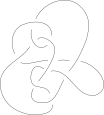
\includegraphics[scale=.3]{figures/intro/hard-unknot.pdf}
  \caption{A ``hard'' unknot}
\end{figure}
Although perhaps not immediately obvious, this is an unknot. To see
this, note that the strand going horizontally across the middle of the
knot can be pulled up behind the arc at the top, tucked down through
the same arc, and then out through the middle arc, at which point one
can apply a Reidemeister II move followed by a reidemeister I move to
undo the knot. For a more detailed view using only Reidemeister moves,
see \cite{Kauffman2011Sep}.

One can verify that there are no Reidemeister I or Reidemeister II
moves that we can perform without adding more crossings to the
diagram. What's more, there are actually \emph{no} Reidemeister III
moves available at all. Thus, this is a knot diagram that has to be
made more complicated before it can be reduced, similarly to the
fractions in $\QQ$.

However, there is a key distinction between these two cases. With the
fractions in $\QQ$, it's always fairly obvious what the next step
should be. We scan left-to-right looking for two fully-simplified
sub-expressions we can combine together; if they're both fractions,
then we convert everything to a common denominator. Next, we combine
the numerators, and then finally we simplify. While seemingly not as
efficient as parsing arithmetic expressions in $\ZZ$, we can still
develop a {greedy algorithm} to attack the problem.

By contrast, there seems to be no obvious strategy to determine which
strands we should move first on the unknot shown above --- or at
least, there isn't one that scales well to large knots.\footnote{This
  doesn't mean one does not exist --- but to the author's knowledge,
  nobody has found one yet.} Hence the simplification problem for
knots seems a bit ``harder.''

Now, regarding (2) (``even if there were such a simplification
algorithm, this still wouldn't immediately give us a canonical
representative.''). The problem here is that in $\ZZ$ and $\QQ$, the
normal forms yielded by our simplification algorithms ended up
coinciding with our canonical forms. Thus, after simplifying
completely, we could simply check for literal equality. This is not
always the case with Knots.%  {\color{blue} We will give a more general
  % strategy for constructing counterexamples later, but the idea is
  % something like this:}
\begin{figure}[H]
  \centering
  \includegraphics[scale=.6]{figures/fundamentals/sum-at-0.pdf}
\end{figure}
\begin{figure}[H]
  \centering
  \includegraphics[scale=.6]{figures/fundamentals/sum-at-3.pdf}
  \caption{Two drawings of the same knot.}
\end{figure}
The reader can verify that these diagrams contain the same number of
crossings. It is harder to see why they are equivalent, though the way
we've drawn them might be suggestive of an argument.\footnote{If the
  reader would like to give this a shot, we heavily encourage a more
  hand-wavey proof that does \emph{not} attempt to employ the
  Reidemeister moves.} It is known that the diagrams above are in
normal form (in that they achieve the minimal crossing number),
although we will not discuss the details in this document.
% {\color{blue} Really I'm just assuming the connected sum crossing
% conjecture and figuring that if this were a counterexample it'd be
% known already.}
In any case, we see that for knots, \np{normal form}
$\nRightarrow$ \np{canonical form}.

Taken in tandem, these problems make approaching the knot equivalence
problem quite challenging. However, there's one saving grace: if we
only want coarse, back-of-the-envelope heuristics for determining
whether two knots are ``probably'' equivalent, then we can actually
employ strategies similar to those used in $\ZZ, \QQ$. This is the
motivation for \emph{invariants.}

\section{Invariants, Briefly.}\label{sec:invariants-briefly}
Hey you --- {\bfseries Think fast!} In 10 seconds or less, which of
the following are true?\footnote{\ldots I'm counting.}
\begin{leftbar}
  \begin{enumerate}[leftmargin=2em]
      \small
    \item $5\pn{3^3 \cdot 11}^2 = 2 (72 + 33 - 8)$
    \item $\displaystyle -\frac{2}{\pn{\sqrt{47} +
      \frac{1}{47}}^{3}} = 47 - \frac{1}{47^2}$
    \item $\displaystyle 3x^4 + (x + 3)(x^2 + 2x + 2) +
      \frac{2}{3}(x - x^2) = 2\pn{x^4 + \frac{3}{2}x(x^2 - 3x)} +
      3x$
  \end{enumerate}
\end{leftbar}
Ok, hopefully that was far too little time to actually figure them all
out. As it turns out, they are all false. Here are some short
arguments for why:
\begin{leftbar}
  \begin{enumerate}
    \item Note that all the factors on the left side ($5$, $3$, $11$)
      are odd, while the right has a leading factor of $2$. So they're
      not equal.
    \item Observe that the left side is negative, while the right side
      is positive (since $47 > 1 > \frac{1}{47^2}$).
    \item This one takes more time to verify, but the leading
      coefficients don't match ($3$ and $2$, respectively). Also, the
      right side has no constant term, whereas the left side does.
  \end{enumerate}
\end{leftbar}
Implicitly, each of these are using an \emph{invariant} of arithmetic
strings. For 1., we know that if two expressions are equal, then if
one is even, the other must be even too. For 2., we are using the fact
that equivalent expressions must have the same sign. And for 3., we
use an invariant of polynomials --- namely that when simplified, their
coefficients must match up.

We can define similar invariants for many other problems. It's worth
noting that these don't always look like simple arithmetic properties,
as demonstrated by the following example:
\begin{example}\renewcommand{\qedsymbol}{}\label{ex:chessboard}
  Consider a $7\times 7$ chessboard with a knight placed on each
  square. Is there a way to move each night exactly once such that
  after each knight has been moved, no knight has left the board, and
  no knights have doubled up on the same square?
  \begin{figure}[H]
    \centering
    \includegraphics[scale=.75]{figures/fundamentals/chessboard.pdf}
    \caption{Diagram of the Situation}  % \qedhere
  \end{figure}
\end{example}
There is an extremely short solution. To emphasize just \emph{how}
short, we've included a redacted version of a short proof by one J.\
Yossarian, just to taunt the reader (an unredacted version can be
found in \cref{sol:chessboard}, \cpageref{sol:chessboard})
\begin{leftbar}
  \emph{Claim:} \censor{No.}\\

  \noindent \emph{Proof:} \censor{Observe that there} are \censor{25
    black squares} and \censor{24 white squares}. \censor{Also}
  \censor{note that every legal move takes} a \censor{knight to} an
  \censor{opposite-color square}. \censor{Hence} \censor{after moving
    all} the \censor{knights}, \censor{we}'\censor{d have 25 on black}
  and \censor{24 on white}, \censor{which is} a
  \censor{contradiction}. \hfill \censor{$\jiong$}
\end{leftbar}
Likewise, many of the invariants we employ in Knot Theory are hard to
connect to explicit algebraic structures we understand. Here are some
high-level examples --- we won't be studying invariants directly, so
don't worry too much about the details, the point is just to know that
they exist.
\begin{example}[Biquandles]
  Let $X$ be a set and $K$ be a knot represented by some diagram $D$.
  Label (``color'') each arc in $D$ by an element of $X$. Then, define
  two binary operations $\underop, \overop$ (read ``under'' and
  ``over,'' respectively) that describe how our labels change when
  strands cross.\footnote{Technically the words here are in the wrong
    order --- we aren't actually guaranteed that such operations exist
    if we begin with an \emph{arbitrary} coloring. But this is meant
    to capture the high-level overview of what the biquandle axioms
    seek to do, so we'll leave it like this for today.}
  \begin{figure}[H]
    \centering
    \includegraphics[scale=.7]{figures/fundamentals/biquandles.pdf}
    \caption{Example of a colored crossing}
  \end{figure}
  By translating the Reidemeister moves into algebraic axioms for
  $\underop, \overop$, we can turn ``coloring by $X$'' into a knot
  invariant:\footnote{The biquandle axioms can look somewhat
    intimidating at first, but with the right diagrams, one can see
    that they are direct translations of the reidemeister moves. We
    haven't included such diagrams since again, we won't really be
    working with biquandles, but for more we encourage the reader to
    reference \cite{NelsonBook}, which we found to be an excellent
    resource.}
  \begin{enumerate}
    \item For all $x \in X$, $x \underop x = x \overop x$,
    \item For all $x,y \in X$, the maps $\alpha_y, \beta_y : X \to X$
      and $S : X \times X \to X \times X$ defined by
      \[
      \alpha_y(x) = x \overop y, \quad \beta_y(x) = x \overop y \quad
      \text{and} \quad S(x,y) = (y \overop x, x \underop y)
      \]
      are all invertible, and
    \item For all $x,y,z \in X$, we have the following \emph{exchange
      laws}:
      \begin{align*}
        (x \underop y) \underop (z \underop y)
        &= (x \underop z) \underop (y \overop z) \\
        (x \underop y) \overop (z \underop y)
        &= (x \overop z) \underop (y \overop z) \\
        (x \overop y) \overop (z \overop y)
        &= (x \overop z) \overop (y \underop z)
      \end{align*}
  \end{enumerate}
  In this case we call $(X, \underop, \overop)$ a \emph{biquandle}.
\end{example}
Biquandles are an example of \emph{coloring invariants}, which are
currently a popular area of study. Another example of a well-known
class of knot invariants is the family of \emph{knot polynomials}.
Knot polynomials are generally agreed to be some of our most powerful
invariants, combining ease of computation with relatively good
performance in distinguishing between knots. An example is the
celebrated \emph{Jones polynomial}, which can be recursively computed
from a knot diagram using the \emph{Kauffman Bracket}:
\begin{example}[Jones Polynomial]
  Define a map $\bk{\ }$ on formal sums of knot diagrams as follows:
  \begin{figure}[H]
    \centering
    \includegraphics[scale=.55]{figures/fundamentals/jones-polynomial.pdf}
    \caption{Kauffman Bracket}
  \end{figure}
  where the diagram is unchanged outside of the dotted neighborhood.
  After applying the bracket map until there are no crossings
  remaining, we're left with a formal sum whose terms are diagrams of
  some number of unlinked unknots. For each such term, apply the
  following conversion:
  \begin{figure}[H]
    \centering
    \includegraphics[scale=1]{figures/fundamentals/jones-delta.pdf}
    \caption{Converting unknots to polynomial terms}
  \end{figure}
  Now every term is a Laurent polynomial in $x$. Combine them all and
  and simplify to yield the \emph{Jones} polynomial.\footnote{This
    process is easier to follow by looking at some examples; the
    reader is encouraged to do so. This is also covered in
    \cite{NelsonBook}; an approach that combines knot polynomials
    \emph{with} coloring invariants like biquandles can be seen in
    \cite{Nelson2017Feb}.}
\end{example}
The Jones Polynomial has many remarkable properties; the reader is
encouraged to poke around through some of the literature on it.

\subsection{Fantastic Invariants \& Where to Find Them}
The section above is meant to highlight two main points: First,
invariants are helpful. We did not discuss explicit performance
metrics, but it is safe to say that employing them is generally much
easier than doing a brute-force search with Reidmeister moves. Second,
powerful invariants can look very different from each other.
Biquandles and the Jones polynomial both operate on diagrams, but do
so through very different mechanisms. This can make it tricky to
identify where we should look \emph{next} for new invariants, since it
can be hard to interpret exactly what structure they are preserving.
What other strategies can we try?

There are two main ways to approach this problem. First, we can try
and generalize the strategies that we know work to see if we can get
modified versions that perform better. A lot of interesting work goes
on here currently, including some of our own results on more general
methods for combining coloring invariants with knot polynomials
(\cite{Kobayashi2019Sep}). However, there is also a more direct
strategy---if we can find ways to describe algebraic structure in the
Knot category more explicitly, we might be able to understand
invariants from a more functorial perspective. Currently, this is
generally avoided, since the structure of the Knot category is not
very well-understood. However, there is one interesting approach that
has yielded some preliminary results recently, which is to make use of
unknotting moves.

Unknotting moves are operations on a diagram that can be used to
reduce arbitrary knots to the circle (an example is being allowed to
``flip'' which strand is on top at any given crossing). Observe that
for an arbitrary knot $K$, playing a sequence of unknotting moves for
$K$ in reverse gives us a way to create $K$ out of an unknotted
circle. Hence, there is a sense in which unknotting moves encode the
information of how to build a knot, and so it seems plausible that
examining them could give us insights into our invariants.

The literature contains precedent for this idea; for instance, it has
been shown that an unknotting move called the \emph{delta move}
affects some polynomial invariants in predictable ways (see
\cite{Kanenobu2005Jan}, \cite{Ganzell2014Feb}). However, there has
been little analysis of the effects of other kinds of unknotting
moves, the effects of performing multiple moves in succession, and
whether the results found can be generalized to other kinds of
invariants. So, in general, the idea remains largely unexplored.

Our motivating goal for this project was to try and attack the problem
of using unknotting moves to define a group-like structure on knots.
The hope is that if we can do so, it will make it easier to search for
powerful invariants by looking at something more homomorphism
flavored.


% As discussed in the overview, pursuing this idea


% and see if tuning some parameters can get us stronger
% results.\footnote{This makes it sound a lot less impressive than it
%   is! Lots of interesting work goes on here.}




%%% Local Variables:
%%% TeX-master: "../../kobayashi-thesis"
%%% End:


\chapter{Knots and Knot diagrams}\label{chap:knots-and-knot-diagrams}
\setlength\epigraphwidth{.7\textwidth}
\epigraph{and an ocean tumbled by with a private boat for Max\\
and he sailed off through night and day\\
and in and out of weeks\\
and about over a year\\
to where the wild things are.}{---Maurice Sendak, \emph{Where the Wild
Things Are}}
The material here is targeted at readers with a basic background in
topology. Experts are advised to skim (or even skip).

% Before we start, a quick note for the reader who is already
% experienced with knot theory:\vspace{.5em}
% % \begin{adjustwidth}{1em}{}
%   \begin{leftbar}
%     \textbf{A word on convention:} In the below, we will define a
%     \emph{knot} to be an embedding of a circle into an arbitrary
%     topological space. This represents a significant break from the
%     usual convention, which is to define a knot as an embedding into
%     either $\RR^3$ or $S^3$. The justification for this decision is
%     that we want to avoid backpedalling when defining \emph{virtual
%       knots}.\\

%     \noindent \textbf{Recommendation on what to read:} We define knots
%     in \cref{sec:KnotDef} and ambient isotopy in \cref{sec:KnotEq};
%     both of these can probably be skipped. In \cref{sec:KnotDiags}, we
%     define the concept of a \emph{diagramming scheme}, which isn't
%     emphasized in most resources. We recommend even the experienced
%     reader skim this part.
%   \end{leftbar}
% % \end{adjustwidth}
% Anyways, on to the introduction.

% {\color{red} Come back and revise to not rely on talking about 3D
%   objects. Also come back and add page references for things}

Knots are fundamentally 3D objects. Studying 3D objects can be hard,
so we'd much rather work with 2D representations if possible.
\emph{Knot diagrams} facilitate this process. The idea is that placing
strict requirements on what we call a ``knot diagram'' allows us to
translate results about these 2D objects to ones for the actual knots.
It's important to be very explicit about how we do this, as the
restrictions we place on our diagrams will dictate what families of
knots we can study with them. The goal for this chapter is to give the
reader intuition for this process.

Our exposition is structured as follows: First, we give the formal
definition of a knot and discuss some of its equivalent versions
(\cpagerefrange{sec:KnotDef}{sec:KnotEq}). We also offer some
intuition for why each requirement in the definition is necessary.
Next, we introduce the standard equivalence relation on knots, which
is known as \emph{ambient isotopy}
(\cpagerefrange{sec:KnotEq}{sec:polygonal-knots}). In doing so, we
first examine two other definitions of equivalence that seem
reasonable but turn out to be flawed (\emph{homeomorphism} and
\emph{non-ambient isotopy}, respectively). Finally, we define
\emph{knot categories} and their associated \emph{diagram categories}.
This offers a nice segue into the next chapter, which discusses the
most common knot category/diagram category pair: \emph{polygonal
  knots} and \emph{regular diagrams}.

\section{Definition of a Knot}\label{sec:KnotDef}
We have to define knots before defining knot diagrams. But to make our
the definition tangible, we need to draw pictures. Hence, we'll have
to make use of knot diagrams before we've actually defined them. The
reader shouldn't worry about this, since it turns out most of the
things we'll need to address in our formal treatment of knot diagrams
are edge cases.

Recall, the intuitive description of a knot that we gave earlier
(\cref{fig:knotcons} on \cpageref{fig:knotcons}) involved taking a
rope, twisting it around in space, and then fusing the ends to get a
closed loop. Importantly, the strand remained ``unbroken'' (in the
sense that there were no cuts in the rope anywhere), and never passed
through itself. This is encoded in the following definition.
\begin{definition}[Topological Knot]\label{def:GenKnotInt}
  Let $(X, \ms T)$ be a topological space. Then a \emph{knot} is a
  continuous map $K : [0,1] \to X$ such that $K$ is injective on
  $[0,1)$, and $K(0) = K(1)$.
\end{definition}
% {\color{red} Let's maybe revise this to be in terms of embeddings}
We'll discuss the importance of the choice of codomain $(X,\ms T)$
later on. But first, to build intuition, we'll restrict our analysis
to the case where $(X, \ms T)$ is $\RR^3$ with the standard topology
(denoted $\ms T_{\rm std}$). This gives us the field of
\emph{classical knot theory}, whose objects of study are
\emph{classical knots}.\footnote{Some authors choose to use $S^3$
  instead of $\RR^3$ because $S^3$ is compact. We won't worry about
  this distinction today.% The interested reader might look into the
  % \emph{Alexandroff extension}, which gives the relationship between
  % $\RR^3$ and $S^3$.
}

\subsection{Classical Knots}
Most of the intuition from $\RR^3$ generalizes to the other choices of
$(X, \ms T)$ we'll be interested in. We just chose to examine the
special case of \emph{classical knots} first to decrease the number of
moving parts in the definition.
\begin{definition}[Classical Knot]\label{def:ClassKnotInt}
  A \emph{classical knot} is a topological knot where $(X,\ms T)$ is
  $(\RR^3, \ms T_{\rm std})$.%  More explicitly, a classical knot is a
  % continuous map $K : [0,1] \to \RR^3$ such that $K$ is injective on
  % $[0,1)$ and $K(0) = K(1)$.
\end{definition}
\begin{aside}
  The choice $[0,1]$ is arbitrary; we could modify our definition to
  use any interval $[a,b]$ and still get a topologically equivalent
  framework. Similarly, choosing $K$ to be injective on $[0,1)$ vs
  $(0,1]$ is also arbitrary since we have $K(0) = K(1)$. We'll remove
  these annoyances later with an equivalent definition in terms of
  $S^1$, but first, let's talk about what this definition is doing.
\end{aside}

First, the codomain is $\RR^3$, so we get an object that lives in 3D
space like we want. Second, we do indeed get a ``loop;'' we can think
of the the domain $[0,1]$ as parameterizing how far along a 1D path we
are.\footnote{You might wonder if space-filling curves would cause
  problems here. It turns out they won't, since we would need to
  loosen one of \{injectivity, continuity\} to get one.} As an
example, if we had $K(t) = (\cos(2\pi t), \sin(2\pi t), 0)$, then
looking down along the $z$ axis and playing time forwards, we would
see something like the following:
\begin{figure}[H]
  \centering
  \includegraphics[scale=1.4]{figures/background/dist-along-knot.pdf}
  \caption{Analogy for the domain}
  \label{fig:DomainAnalogy}
\end{figure}
\noindent Here, the inner ring shows $K(t)$ itself, while the outer
ring is just showing us a reminder of what the corresponding values of
$t$ are.

Next, note that requiring $K$ be \emph{continuous} and $K(0) = K(1)$
prevents us from getting any ``breaks'' in the strand (a rope wouldn't
make a good knot if it had a cut in it); see \cref{fig:KnotBreak}
below. Similarly, the injectivity condition prevents us from getting
self-intersections in our rope; see
\cref{fig:SelfIntersect} below.\\
\begin{minipage}{.49\linewidth}
  \begin{figure}[H]
    \centering
    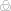
\includegraphics[scale=.15]{figures/background/broken-trefoil.pdf}
    \caption{A ``knot'' with a break in it}
    \label{fig:KnotBreak}
  \end{figure}
\end{minipage}
\begin{minipage}{.49\linewidth}
  \begin{figure}[H]
    \centering
    \includegraphics[scale=.3]{figures/background/self-intersect.pdf}
    \caption{A ``knot'' with points of self-intersection (black)}
    \label{fig:SelfIntersect}
  \end{figure}
\end{minipage}\\[1em]
To see that the ``knot'' in \cref{fig:SelfIntersect} really \emph{can}
be realized as a continuous function $K : [0,1] \to \RR^3$ (and thus
the injectivity condition is strictly necessary), consider the
following construction: % {\color{red} rewrite me}
\begin{figure}[H]
  \centering
  \includegraphics[scale=.8]{figures/background/self-intersect-cons.pdf}
  \caption{Example of how we'd construct the self-intersecting ``knot''}
\end{figure}
\noindent Hence we see we need all of the pieces of the definition
given.
% \noindent\hrulefill

\subsection{Equivalent Definition in terms of $S^1$}
% {\color{red} Maybe we also wanna talk about general $[a,b]$}

Okay: \cref{def:ClassKnotInt} is fine and intuitive, but as alluded to
before, it can be written more succinctly. In particular, the whole
``injective on $[0,1)$ and $K(0) = K(1)$ except you could also use
$(0,1]$'' part can be done away with by gluing the ends of $[0,1]$
together to get a circle. This motivates the second definition, which
is more commonly used.

\begin{definition}[Classical Knot, redux]\label{def:ClassKnotS1}
  A \emph{knot} is an injective, continuous map $K : S^1 \into \RR^3$.
\end{definition}
Note, since we already identify $0$ and $1$ in $S^1$, we don't have to
state the extra injectivity conditions. We'll use this definition
throughout the rest of this document.%  {\color{red} Come back and talk
  % about how we did away with the arbitrary interval part by
  % precomposing with a homeomorphism.}

It is straightforward to show that this is equivalent to the previous
definition. Here's the strategy: let $K : [0,1] \to \RR^3$ be a knot
(in the sense of the first definition), and let $\pi$ be the quotient
map $\pi : [0,1] \to [0,1]/\set{0 \sim 1}$. Then show that there
exists a unique continuous $K' : S^1 \into \RR^3$ such that the
following diagram commutes:
\begin{figure}[H]
  \centering
  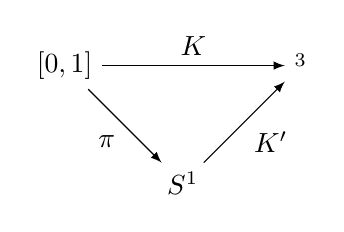
\begin{tikzpicture}
    \node (a) at (-1.5,0) {$[0,1]$};
    \node (b) at (0,-1.5) {$S^1$};
    \node (c) at (1.5, 0) {$\RR^3$};

    \draw[-latex] (a) -- (b) node[midway, below left] {$\pi$};
    \draw[-latex] (a) -- (c) node[midway, above] {$K$};
    \draw[-latex] (b) -- (c) node[midway, below right] {$K'$};
  \end{tikzpicture}
  \caption{Commutative diagram}
\end{figure}
This is straightforward enough that it might seem silly to state
explicitly, but it is cool to see it in action. Check out
\href{https://youtu.be/7cDroN4n8EQ}{https://youtu.be/7cDroN4n8EQ} for
an example animation.
\begin{example}
  The following is a knot known as $(7,2)$.
  \begin{figure}[H]
    \centering
    \includegraphics{figures/background/embed-72.pdf}
    \caption{The $(7,2)$ knot}\qedhere
  \end{figure}
  \label{ex:72knot}
\end{example}
The name $(7,2)$ convention comes from the fact that 7 is the minimum
number of crossings we can have in a diagram for the knot. The 2 is
just a label dictated by convention so that we know \emph{which} of
the 7-crossing knots we're dealing with.\footnote{For a gallery of the
  so-called \emph{prime} knots up to a given crossing number, see
  \href{http://katlas.math.toronto.edu/wiki/The_Rolfsen_Knot_Table}{http://katlas.math.toronto.edu/wiki/The\_Rolfsen\_Knot\_Table}}

There is a sense in which knots act like homeomorphims. In particular,
for a knot $K$, the \emph{image} of $S^1$ under $K$ is still a closed
loop (and in fact, this loop is homeomorphic to $S^1$). But since $K$
is not a bijection ($K$ is not not onto $\RR^3$), we can't call it a
homeomorphism. We can, however, call it an embedding.
\begin{definition}[Embedding]
  Let $(X,\ms T)$, $(Y, \ms S)$ be topological spaces, and let $f : X
  \to Y$. Then we say $f$ is an \emph{embedding} iff $f$ is a
  homeomorphism between $X$ and $f(X)$, where $f(X)$ is given the
  subspace topology from $Y$.
\end{definition}

\begin{proposition}\label{prop:knots-are-embeddings}
  Let $K : S^1 \into \RR^3$ be a knot. Then $K$ is an
  \emph{embedding}.
\end{proposition}
\begin{proof}
  % The following is based on a stackexchange thread. \footnote{See
  %   \href{https://math.stackexchange.com/questions/474693/if-we-have-an-embedding-fx-rightarrow-a-where-a-subset-y-do-we-have-to}{https://math.stackexchange.com/questions/474693/if-we-have-an-embedding-fx-rightarrow-a-where-a-subset-y-do-we-have-to}}

  We want to show $K$ is a homeomorphism between $X$ and $K(X)$. Note,
  any injective function is bijective with its image, so $K$ is a
  bijection between $X$ and $K(x)$. Now, the definition of a knot
  guarantees $K$ is continuous. Given these conditions, one can show
  that it suffices to prove $K$ is a closed map (i.e.\ image of a
  closed set is closed).

  Let $A \subseteq S^1$ be closed. Since $S^1$ is compact, it follows
  that $A$ is compact. Since $K$ is continuous, it follows that $K(A)$
  is compact. Now, since $\RR^3$ is Hausdorff, all compact sets are
  closed. Hence $K(A)$ is closed, so $K$ is a closed map, and thus a
  homeomorphism (as desired).
\end{proof}

\subsection{Other Codomains}
We want to take a moment to stress that the choice of codomain is a
hugely important factor in determining the behavior of our knots.
Knottedness (as a general phenomenon) \emph{fundamentally} arises out
from taking a small space and trying to find ways to fit into a
slightly larger one. Here, we've taken $S^1$ (a 1-manifold) and stuck
it into $\RR^3$, but one might wonder whether we'd get different
theories if we tried, say, $\RR^2$, $\RR^4$, or $\RR^n$.

It turns out that we do. In both $\RR^2$ and $\RR^4$, \emph{all} knots
turn out to be equivalent to each other. The intuition is a bit
different in $\RR^2$ than in $\RR^4$, however. We'll examine the
$\RR^2$ case in more detail during \cref{chap:ambient-isotopy-in-r2},
but the loose idea is that $\RR^2$ ``confines'' our embedded copy of
$S^1$ too tightly to allow it to get all tangled up (indeed, the
string can't cross itself when restricted to $\RR^2$). In $\RR^4$, we
see the opposite phenomenon. Because we have a whole extra spatial
dimension to work with, the string can never quite get ``stuck'' on
itself in $\RR^4$ --- there's always a sneaky way to get around the
barrier.\footnote{We have some slides posted at
  \url{https://bedmathandbeyond.xyz/files/kaestner-brackets.pdf} with
  a small visualization, but the reader should look elsewhere for a
  detailed explanation.}

Interestingly, things of this flavor turn out to be a fairly general
phenomenon --- given a ``tame'' $n$-manifold $N$ and an $m$-manifold
$M$ (with some additional niceness constraints), if $n - m \neq 2$,
the embedded copy of $M$ in $N$ is often easy to unknot. However, when
we have equality ($n = m-2$), things can get hairier. The interested
reader is encouraged to read more in \cite{Daverman}, but be warned,
the content is very prerequisite-heavy.

Anyways, in light of the trivial behavior in $\RR^2$ and $\RR^4$, the
only other codomains we'll look at here will be \emph{thickened
  orientable surfaces}. These yield \emph{virtual knot theory}, which
we will discuss in \cref{sec:virtual-knots}. Until then the reader
should just assume we're always thinking about knots from $S^1 \into
\RR^3$.
% Hence, the main other focus of knot theory
% Let's

% \begin{itemize}
%   \item Relationship of knots to the fundamental group
%   \item Virtual knots
%   \item Knots in $\RR^2$
% \end{itemize}

% {\color{red} Come back and put in a transition}

\section{Knot Equivalence}\label{sec:KnotEq}
We'll now go about formalizing what it means for two knots $K_0, K_1$
(oriented or unoriented) to be \emph{the same}. On an intuitive level,
we want our definition to capture the idea that if we were to tie a
rope up in the shapes of $K_0, K_1$, then $K_0$ would be ``equivalent
to'' $K_1$ iff by playing with the rope for long enough, we could find
a way to make $K_0$ look exactly like $K_1$ (without just cutting the
string apart and gluing it back together). We seek a way to make this
idea formal. We'll discuss two definitions that turn out to fail
before introducing the correct one.
\begin{attempt}[Homeomorphism]
  Let $K_0, K_1$ be knots. Then we say $K_0$ and $K_1$ are
  \emph{equivalent} iff there exists a homeomorphism between their
  images.
\end{attempt}
This does not work. In particular, since $K_0, K_1$ are embeddings,
their images are always homeomorphic to $S^1$, and thus to each other.
So this would make \emph{all} knots equal, which we don't want to have
happen. Here's a much better idea: what if we defined $K_0$, $K_1$ to
be equivalent if we can find a continuous ``path'' through
intermediate knots that get us from $K_0$ to $K_1$? This is captured
by \emph{isotopy}:
\begin{attempt}[Isotopy]
  Let $K_0, K_1 : S^1 \into \RR^3$ be knots. Then we define an
  \emph{isotopy} from $K_0$ to $K_1$ to be a function $H : [0,1]
  \times X \to Y$ such that
  \begin{enumerate}
    \item For all $x \in X$, $t \in [0,1]$, the map $H_t(x) = H(t, x)$
      is an embedding,
    \item For all $x \in X$, we have $H( 0, x) = K_0(x)$ and
      $H(1, x) = K_1(x)$, and
    \item $H$ is continuous. \qedhere
  \end{enumerate}
\end{attempt}
Note, condition (1) guarantees that we take a ``path'' through other
embeddings. Condition (2) requires that this ``path'' start at $f$ and
end at $g$. Condition (3) guarantees that the path doesn't have any
``jumps.''

This almost works, but there's a small hiccup that breaks this
definition as well. The reader might take a moment to try and identify
the issue. Here's some food for thought: Homeomorphism put all knots
into the same equivalence class. Does isotopy do the same? Or does it
distinguish some families of knots? Which ones?

As it turns out, this definition also puts all knots in the same
equivalence class. Here's some intuition: Let $x \in X$ be fixed.
Because the continuity condition on $H$ only requires $\forall
\varepsilon > 0$, there exists $\delta > 0$ such that $d(K(t, x), K(t
+ \delta, x))$, we can get two arbitrary embeddings $K_0$, $K_1$ to be
equivalent to each other by just ``shrinking all the differences down
to an arbitrarily small region'' An example for the trefoil (known as
\emph{Bachelor's unknotting}) is shown below.
% The reader is encouraged
% to

% The idea the idea is to define an isotopy
% like the following:
% . In particular, we can't
% necessarily show that arbitrary $K_0$ and $K_1$ are now
% ``equivalent,'' but we \emph{can} show that an arbitrary $K_0$ is
% equivalent to the unknot. The idea is to define our isotopy like the
% following:
\begin{figure}[H]
  \centering
  \includegraphics[scale=2]{figures/background/bachelor-unknotting.pdf}
  \caption{Bachelor's unknotting}
\end{figure}
% \noindent Using this, one can argue that arbitrary $K: S^1 \into
% \RR^3$ is isotopic to the unknot.
By shrinking down the region in which the crossings occur, we have
found an isotopy removing all of the crossings of the trefoil. Note,
we could even play it in reverse, and spontaneously generate a trefoil
out of an unknot! Clearly this is undesirable. But we are on the right
track. It turns out the ``correct'' definition will be very similar.
Instead of performing an isotopy on the embeddings themselves, we
perform it on the ambient space. This is known as \emph{ambient
  isotopy}.
\begin{definition}[Ambient Isotopy]
  Let $K_0, K_1$ be knots. Then we say $K_0$ is \emph{ambient
    isotopic} or \emph{equivalent} to $K_1$ iff there exists a map $H
  : [0,1] \times \RR^3 \to \RR^3$ such that
  \begin{enumerate}
    \item For all $\mb x \in \RR^3$, $t \in [0,1]$, the map $H_t(\mb x)
      = H(\mb x, t)$ is a homeomorphism,
    \item For all $s \in S^1$, $H(K_0(s), 0) = K_0(s)$ and
      $H(K_0(s),1) = K_1(s)$, and
    \item $H$ is continuous. \qedhere
  \end{enumerate}
\end{definition}
% \noindent Note the similarity to the definition of isotopy when we
% take $X = Y = \RR^3$.
This turns out to be the ``correct'' notion of equivalence, and with
it, we can begin to partition our knots into equivalence classes.
However, it can often be unwieldy to work with ambient isotopies
directly, as topological embeddings can get quite messy. As such we
often restrict ourselves to a family of knots where ambient isotopy
can be characterized by the \emph{Reidemeister moves}, which affords
us a more combinatorial approach to equivalence. This nice family is
known as the collection of \emph{tame knots}, which are defined in
terms of the even simpler \emph{polygonal knots}. A more careful look
at the definitions of tameness will be given in
\cref{chap:tame-and-wild-knots}.

\section{Tame and Polygonal Knots}\label{sec:polygonal-knots}
% \chapter{Polygonal Knots}\label{chap:polygonal-knots}
In this section, we will (very briefly) examine the ``simplest''
possible knots, \emph{polygonal knots}. If the reader would like a
deeper examination of the topic, they are encouraged to take a look at
\cite{burde2003knots} and \cite{Crowell1963}.

Polygonal knots form the backbone for modern combinatorial knot
theory. The idea is that since they are formed out of finite unions of
straight line segments, they can be studied combinatorially, which
makes them nice. What's a little less obvious is that we can actually
extend some of the resulting ideas to \emph{any} knot ambient isotopic
to a polygonal knot. Indeed, essential results such as
\emph{Reidemeister's Theorem} rely on our knots of interest being
ambient isotopic to polygonal knots.
\begin{definition}[Polygonal Knot]
  A \emph{polygonal knot} $\msf K : S^1 \to \RR^3$ is a knot comprised
  of a finite union of straight line segments.\footnote{Note that we
    will also try to use the \emph{sans-serif} font to distinguish
    polygonal knots from their topological counterparts, since
    sans-serif letters are straight and angular.}
\end{definition}
\begin{figure}[H]
  \centering
  \includegraphics[width=\linewidth]{figures/polygonal-knots/ex-polyknots.pdf}
  \caption{Examples of some polygonal knots}
\end{figure}
It might be helpful to think of polygonal knots in terms of finite
sequences of vertices. This really hammers home the idea that
polygonal knots can be encoded with finite information.
\begin{example}
  We would write the following knot as $\msf{K} = \pn{\msf{v_1, v_2,
      v_3, v_4, v_5, v_6, v_7}}$, where each $\msf{v_i} \in \RR^3$.
  \begin{figure}[H]
    \centering
    \includegraphics{figures/polygonal-knots/4-1-labeled.pdf}
    \caption[Labeled polygonal $\msf{(4,1)}$]{Polygonal $\msf{(4,1)}$
      knot with vertices labeled} \qedhere
  \end{figure}
\end{example}
The promised combinatorial niceness comes from the following theorem:
\begin{theorem}\label{thm:polygonal-ambient-isotopy}
  Let $\msf K_0, \msf K_1 : S^1 \into \RR^3$ be polygonal knots. Then
  $\msf K_0 \cong \msf K_1$ iff there exists an ambient isotopy $\msf
  F : [0,1] \times \RR^3 \to \RR^3$ with $\msf F(1, \msf K_0) = \msf
  K_1$ that can be realized entirely through a finite sequence of the
  two \emph{elementary moves} (note, in the below, the dashed lines
  are draw somewhat arbitrarily --- we don't really care what the knot
  looks like away from our local picture):
  \begin{enumerate}[label=\arabic*)]
    \item Subdivision:
      \begin{figure}[H]
        \centering
        \includegraphics[scale=.85]{figures/fundamentals/el-move-1.pdf}
        \caption[Elementary move 1]{Elementary move 1: adding or
          deleting a vertex}
      \end{figure}
    \item Kinking (note, we require that no line segment passes
      through the triangle in $\RR^3$ with vertices $v_a, v_b, v_c$):
      \begin{figure}[H]
        \centering
        \includegraphics[scale=.85]{figures/fundamentals/el-move-2.pdf}
        \caption[Elementary move 2]{Elementary move 2: swapping edges
          on a triangle}
      \end{figure}
  \end{enumerate}
\end{theorem}
\begin{remark}
  It's worth emphasizing that although we've drawn the moves above to
  appear planar, they're really happening in $\RR^3$. So we
  \emph{could} have all sorts of things happening above or below our
  region of interest. We just need to require that there are no
  obstacles in performing the kink move.
\end{remark}
We will not offer a proof of the theorem, since working with ambient
isotopy directly turns out to be somewhat of a headache, and the proof
won't be terribly informative for the contexts we \emph{do} interact
with ambient isotopy in later on. The point is just to illustrate how
simple ambient isotopy is for polygonal knots.

We now define \emph{tame knots} from polygonal knots.
\begin{definition}[Tame Knot]
  Let $K : S^1 \into \RR^3$ be a knot. Suppose that there exists a
  polygonal knot $\msf K : S^1 \into \RR^3$ such that $K \cong \msf
  K$. Then we say \emph{$K$ is a tame knot}.
\end{definition}
We call knots that are not tame \emph{wild} knots. Little is known
about wild knots; they are the focus of \cref{part:wild-knots}.
\begin{figure}[H]
  \begin{minipage}{.49\linewidth}
    \begin{figure}[H]
      \centering
      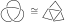
\includegraphics{figures/background/polygonal-knot.pdf}
      \caption{Example of a tame knot}
    \end{figure}
  \end{minipage}
  \begin{minipage}{.49\linewidth}
    \vspace{1.25em}
    \begin{figure}[H]
      \centering
      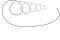
\includegraphics[scale=.6]{figures/background/wild-knot-example.pdf}
      \caption{Example of a wild knot (the loops repeat infinitely)}
    \end{figure}
  \end{minipage}
\end{figure}
The next step in constructing our theory is to state Reidemeister's
theorem for tame knots, which will allow us to turn the 3D moves in
\cref{thm:polygonal-ambient-isotopy} into purely 2D moves on diagrams.
In order for this to work, we need our diagrams to give us enough
information to reconstruct everything that's going on in $3$D up to
ambient isotopy.
% This is the focus of the next section is on understanding knot
% diagrams and why they're special.
% Now Reidemeister's theorem follows from


 % However,
% \cref{thm:all-ambient-isotopic-in-r2} from \cref{part:wild-knots}



% In building up our theory of knots, it will be useful to employ two
% distinct equivalence relations on polygonal knots. The first (known as
% \emph{planar isotopy}) is finer than the second (which I will refer to
% as \emph{polygonal ambient isotopy}).\footnote{Here, ``finer'' means
%   that planar isotopy breaks polygonal knots into more equivalence
%   classes than polygonal ambient isotopy does. This does not imply
%   that planar isotopy is the more ``natural'' choice for definign
%   equivalence of polygonal knots; as we will see, polygonal ambient
%   isotopy corresponds more directly with the general definition of
%   ambient isotopy that we gave before.} However, this granularity
% comes at a price --- planar isotopy doesn't allow us to change any
% crossings. As such, we can't say the following knots are equivalent by
% planar isotopy:
% \begin{figure}[H]
%   \centering
%   \includegraphics[scale=.5]{figures/polygonal-knots/non-planar-isotopic-example.pdf}
%   \caption[Ambient isotopic but not planar isotopic]{Two polygonal
%     knots that are not planar isotopic}
% \end{figure}
% {\color{red} if choosing to use $\equiv$ exclusively for planar
%   isotopy, add this to the preface}

% {\color{red} come back and talk about polygonal knots vs polygonal
%   knot diagrams}

% {\color{red} come back and change the word ``involved'' to
%   ``incident'' or something and define that elsewhere}

% Ok, now the definitions.
% \subsection{Elementary Moves}
% Elementary moves are the building blocks for {\color{red} a bunch of
%   stuff. Let's define them.}
% \begin{definition}[Elementary Moves]
%   Let $\msf{K} = \pn{\msf{v_1, \ldots, v_n}}$ be a polygonal knot.
%   Then an elementary is an insertion/deletion of a vertex in $\msf K$
%   as follows:
%   \begin{enumerate}
%     \item Suppose {\color{red} return to this}
%     \item
%   \end{enumerate}
% \end{definition}

% \subsection{Planar Isotopy}
% Planar isotopy is based on the idea of a \emph{planar move}. These
% are special elementary moves that
% \begin{definition}[Planar Moves]\label{def:planarmoves}
%   Let $\msf{K = \pn{v_1,\ldots, v_n}}$ be a polygonal knot. A
%   \emph{planar move} on $\msf K$ corresponds to the insertion or
%   deletion of a vertex in $\msf{K}$ per one of the following cases
%   (see {\color{red} insert ref here} for diagrams):
%   \begin{enumerate}
%     \item Insertion rules: Let $\msf{v_i, v_{i+1}}$ be sequential
%       vertices in $\msf{K}$ and let $\msf{v_{new}} \in \RR^3$.
%       Suppose we have one of the following cases:
%       \begin{enumerate}
%         \item Subdivision: Suppose that $\msf{v_{new}}$ is on the line
%           segment connecting $\msf{v_i, v_{i+1}}$.
%         \item Kink on a free segment: Suppose that the line segment
%           $(\msf{v_i}, \msf{v_{i+1}})$ is not involved in any
%           crossings in $\msf{K}$ and the line segments defined by
%           $\msf{\pn{v_i, v_{new}}}$ and $\msf{\pn{v_{new}, v_{i+1}}}$
%           also aren't involved in any crossings.
%         \item Kink on a crossing
%           segment:\footnote{\label{foot:nonredundant} This is not
%             redundant with the subdivision rule. See {\color{red}
%               Insert ref to remark here} for explanation.} Suppose
%           that the line segment $\pn{\msf{v_i, v_{i+1}}}$ is involved
%           in exactly one crossing in $\msf{K}$. Denote the crossed
%           strand by $\pn{\msf{v_j, v_{j+1}}}$ and suppose that
%           \emph{exactly one} of $\pn{\msf{v_i, v_{new}}}$ or
%           $\pn{\msf{v_{new}, v_{i+1}}}$ crosses $\pn{\msf{v_i,
%               v_{i+1}}}$. Denote this segment by $\msf{e_{cross}}$ and
%           the other by $\msf{e_{free}}$. Finally, suppose that
%           $\msf{e_{cross}}$ crosses over/under $\pn{\msf{v_j,
%               v_{j+1}}}$ iff $\pn{\msf{v_i, v_{i+1}}}$ does, and that
%           $\msf{e_{free}}$ is not involved in any crossings.
%       \end{enumerate}
%       Then in any of these cases, the insertion
%       \[
%         \msf{\pn{v_1, \ldots, v_i, v_{i+1}, \ldots, v_n}} \mapsto
%         \msf{\pn{v_1, \ldots, v_i, {\color{blue} v_{new}}, v_{i+1},
%             \ldots, v_n}}
%       \]
%       is a planar move.
%     \item Deletion rules: These correspond to undoing the moves above.
%       Let $\msf{v_{i-1}, v_{i}, v_{i+1}}$ be sequential vertices in
%       $\msf{K}$; here $\msf{v_i}$ corresponds to $\msf{v_{new}}$
%       above. Suppose that we have one of the following cases:
%       \begin{enumerate}
%         \item Subdivision: Suppose that $\msf{v_i}$ is on the line
%           segment $\pn{\msf{v_{i-1}, v_{i+1}}}$.
%         \item Kink on a free segment: Suppose that none of the line
%           segments defined by $\msf{\pn{v_{i-1}, v_i}, \pn{v_i,
%               v_{i+1}}}$, and $\msf{\pn{v_{i-1}, v_{i+1}}}$ are
%           involved in crossings.
%         \item Kink on a crossing segment: Suppose that exactly one of
%           $\pn{\msf{v_{i-1},v_i}}$ and $\pn{\msf{v_i, v_{i+1}}}$ is
%           involved in a single crossing, and that the other is
%           involved in no crossings. Denote the crossed strand by
%           $\msf{e_{cross}}$, and suppose that $\msf{v_{i-1}, v_{i+1}}$
%           crosses $\msf{e_{cross}}$ in the same way (over if over,
%           under if under).
%       \end{enumerate}
%       Then in any of these cases case, the deletion
%       \[
%         \msf{\pn{v_1, \ldots, v_{i-1}, {\color{blue} v_i},
%             v_{i+1}, \ldots, v_n}} \mapsto \msf{\pn{v_1, \ldots,
%             v_{i-1}, v_{i+1}, \ldots, v_n}}
%       \]
%       is a planar move.
%   \end{enumerate}
% \end{definition}
% \begin{remark}
%   As noted in \cref{foot:nonredundant}, the \emph{subdivision} and
%   \emph{kink on a crossing segment} moves are not redundant. The
%   reason is that \emph{subdivision} is allowed even when multiple
%   strands cross $\pn{\msf{v_i, v_{i+1}}}$, whereas \emph{kink on a
%     crossing segment} doesn't. {\color{red} Is it worth keeping these
%     definitions separate, or should I try and roll them together?}
% \end{remark}

% \begin{figure}[H]
%   \centering
%   \includegraphics[draft]{figures/polygonal-knots/planar-moves.pdf}
%   \caption{Planar moves}
% \end{figure}

% \begin{proposition}
%   Finite sequences of planar moves can never add or remove crossings
%   in a diagram for $\msf{K}$.
% \end{proposition}
% \begin{proof}
%   Each of the three moves defined in \cref{def:planmoves} preserve the
%   number of crossings in $\msf{K}$. The finiteness condition prevents
%   us from getting situations like the following:
%   \begin{figure}[H]
%     \centering
%     \includegraphics[draft]{figures/polygonal-knots/losing-a-crossing.pdf}
%     \caption{Sequence losing a crossing in the limit}
%   \end{figure}
% \end{proof}

% % \begin{proposition}
% %   This implies moves that change \emph{multiple} crossings are ok. But
% %   we will only consider single crossings
% % \end{proposition}
% \subsection{Polygonal Ambient Isotopy and Reidemeister's Theorem}
% We want to develop an equivalence relation that \emph{does} allow us
% to modify crossings. This will be furnished by \emph{polygonal ambient
%   isotopy}, which mirrors the definition of \emph{ambient isotopy} for
% general topological knots.

% Recall that we defined a general ambient isotopy to be a continuous
% deformation of the ambient space that restricts to a homotopy
% \emph{through} knots, starting with $K_0$ and ending with $K_1$.
% {\color{red} come back and revise; this isn't quite right.} We'll
% define polygonal ambient isotopy similarly, only now we require our
% function to restrict to a homotopy through \emph{polygonal knots}.
% \begin{definition}[Equivalence of Polygonal Knots]
%   Let $\msf{K_1}$, $\msf{K_2} : S^1 \to (X, \ms T)$ be polygonal
%   knots. Then we say $\msf{K_1, K_2}$ are \emph{equivalent} or
%   \emph{polygonally ambient isotopic} iff there exists an ambient
%   isotopy $\msf F : X \times [0,1] \to X$ such that for each $t \in
%   [0,1]$, $\msf F(\msf{K_1}, t)$ is a polygonal knot.
% \end{definition}
% We want to be able to characterize polygonal ambient isotopy in terms
% of simple moves like those employed in \emph{planar} isotopy. The
% means to do so are furnished by \emph{Reidemeister's Theorem},
% {\color{red} one of the crowning achievements of knot theory during
%   the early 20\textsuperscript{th} century}. Note, {\color{red} talk
%   about how today we actually prove something from which
%   Reidemeister's Theorem follows as a corollary}

% {\color{red} This next lemma tells us that strands of our knots are
%   separated in some sense }
% \begin{lemma}
%   Let $\msf K$ be a polygonal knot. Let $\msf{e_1, e_2}$ be line
%   segments in $\msf K$ that do not share a vertex (note, this implies
%   $\msf{e_1 \neq e_2}$). Then
%   \[
%     \inf_{\substack{\msf{x_1} \in \msf{e_1} \\ \msf{x_2} \in
%         \msf{e_2}}} d(\msf{x_1, x_2}) > 0.
%   \]
% \end{lemma}
% \begin{proof}
%   We have two cases.
%   \begin{enumerate}[label=\arabic*)]
%     \item Suppose $\msf{e_1}$ is parallel to $\msf{e_2}$. Then since
%       $\msf{e_1} \cap \msf{e_2} = \varnothing$, {\color{red}
%         aaaaaaaaaaaaaaaa this means the distnace is constant between
%         them something something use multi calc if you'd like}
%     \item Suppose $\msf{e_1}$ is not parallel to $\msf{e_2}$.
%   \end{enumerate}

%   Suppose not. Then $\forall \varepsilon > 0$, there exist
%   $\msf{x_{1}} \in \msf{e_1}$ and $\msf{x_{2}} \in \msf{e_2}$ such
%   that $d(\msf{x_1}, \msf{x_2}) < \varepsilon$. Now, consider the
%   sequence
%   \[
%     \varepsilon_n = \frac{1}{n} \qquad\qquad \text{for all }n \in \NN,
%   \]
%   and let $\pn{\msf{x_{1,n}}}_{n\in\NN}$,
%   $\pn{\msf{x_{2,n}}}_{n\in\NN}$ be sequences of points in
%   $\msf{e_1,e_2}$ respectively such that for all $n \in \NN$,
%   $d(\msf{x_{1,n}, x_{2,n}}) < \varepsilon_n$. Now, let
%   \[
%     \msf{x_1} = \lim_{n\to\infty} \msf{x_{1,n}}\qquad \text{and}
%     \qquad \msf{x_2} = \lim_{n\to\infty} \msf{x_{2,n}}.
%   \]
%   {\color{red} Wait how do we know these limits exist?}

%   Note, $\msf{e_1, e_2}$ are line segments in $\RR^3$ and are thus
%   closed. It follows that they are complete, so we have $\msf{x_{1},
%     x_2}$. Hence, Now, $\msf{x_1} = \msf{x_2}$
% \end{proof}

% \begin{corollary}\label{cor:elarepolyamb}
%   Elementary moves are polygonal ambient isotopies.
% \end{corollary}
% \begin{proof}
%   {\color{red} Come back and fill in the details. Just do the
%     straight-line homotopy between the edges}
% \end{proof}

% \begin{theorem}

% \end{theorem}


% \begin{theorem}
%   Let $\msf{K_1, K_2}$ be polygonal knots. Then the following are
%   equivalent:
%   \begin{enumerate}
%     \item $\msf{K_1}$ and $\msf{K_2}$ are polygonally ambient
%       isotopic,
%     \item There exists an orientation-preserving homeomorphism $f :
%       \RR^3 \to \RR^3$ such that $f(\msf{K_0}) = \msf{K_1}$.
%     \item $\msf{K_1}$ and $\msf{K_2}$ are related by a finite sequence
%       of elementary moves,
%   \end{enumerate}
% \end{theorem}
% \begin{proof}
%   We base our exposition on the argument given in
%   \cite{burde2003knots}. We first prove $1 \iff 2$ and then prove $2
%   \iff 3$.
%   \begin{enumerate}[label=(\alph*)]
%     \item We want to show $1 \iff 2$.
%       \begin{iffproof}
%         \item Suppose that $\msf{K_1}$, $\msf{K_2}$ are polygonally
%           ambient isotopic by some $F : \RR^3 \times [0,1] \to \RR^3$.
%           {\color{red} Come back and double check whether we really
%             want $X$ here}. Then taking $f = F(\cdot, 1)$ yields the
%           desired orientation-preserving homeomorphism.
%         \item Suppose that there exists an orientation-preserving
%           homeomorphism $f : \RR^3 \to \RR^3$ such that $f(K_0) =
%           K_1$.

%           \textbf{Claim 1:} There exists an ambient isotopy $F : \RR^3
%           \times [0,1] \to \RR^3$ such that
%       \end{iffproof}
%   \end{enumerate}
% \end{proof}

% \begin{proof}~
%   \begin{iffproof}
%     \item This follows from \cref{cor:elarepolyamb}
%     \item Suppose that $\msf{K_1, K_2}$ are polygonally ambient
%       isotopic, denote the polygonal ambient isotopy by $\msf F$.

%       For each $t \in [0,1]$, $\msf{F}(\msf{K_1}, t)$ is a polygonal
%       knot. Thus, at each time $t$,
%       \begin{itemize}
%         \item Our knot is a finite union of straight line segments
%         \item By continuity, $\forall \varepsilon > 0$, there exists a
%           $\delta > 0$ such that things being within delta of each
%           other make the difference less than $\varepsilon$
%         \item Choose $\varepsilon$ to be $1/2$ of the minimizing
%           distance between points on any two of the line segments
%           making up $K_1$ (such a min exists by finitely many line
%           segments condition).
%         \item This gives us the first set of elementary moves.
%         \item
%       \end{itemize}
%   \end{iffproof}
% \end{proof}

% {\color{red} How are elementary moves realized in the Diagrams??????
%   IDK Reidemeister Theorem time }
% \begin{theorem}
%   \color{red} AAAAAAAAAAAAAAAAAAAAAAAAAAAAAAAAAAAAa
% \end{theorem}



% \section{Tame Knots and Regular Diagrams}

% \begin{theorem}
%   Two knots $K_1, K_2$ are ambient isotopic iff their polygonal
%   representations $\msf{K_1, K_2}$ are polygonally isotopic.
% \end{theorem}

% {\color{red} Insert examples here}

% \begin{definition}[Smooth Knots]
%   AAAAAAAAAAAAAAAAAAAAAAAAa
% \end{definition}

% \begin{definition}[Tame Knots]
%   A knot is called \emph{tame} aaaaaaaaaaaaaaaaaaaaaaaaaaaaa
% \end{definition}

% \begin{definition}[Wild Knots]
%   Give the definition
% \end{definition}







% \section{Regular Diagrams and Reidemeister's Theorem}






% {\color{red} Return and make sure this is integrated well at some
%   point}

% We want to study knots (and the knot equivalence problem) from a
% combinatorial perspective. To do so,



% Now, we can partition knots into two important sets
% Now, we can talk about the difference between so-called \emph{tame}
% knots and \emph{wild} knots.
% Loosely speaking, a diagram of a tame
% knot can be encoded with finite amounts of information, while a
% diagram for a wild knot cannot (we'll talk about this more in the
% next section).
% Knots come in two flavors
% : \emph{tame knots} and \emph{wild knots}. Loosely speaking,
% \emph{tame knots} can be approximated by finitely many straight-line
% segments, while \emph{wild knots} cannot (we discuss this in the next
% chapter).\\
% \begin{minipage}{.49\linewidth}
%   \begin{figure}[H]
%     \centering
%     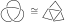
\includegraphics{figures/background/polygonal-knot.pdf}
%     \caption{Example of a tame knot}
%   \end{figure}
% \end{minipage}
% \begin{minipage}{.49\linewidth}
%   \vspace{1.25em}
%   \begin{figure}[H]
%     \centering
%     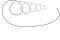
\includegraphics[scale=.6]{figures/background/wild-knot-example.pdf}
%     \caption{Example of a wild knot (the loops repeat infinitely)}
%   \end{figure}
% \end{minipage}\vspace{.5em}
% Currently, we understand tame knots fairly well but know very little
% about wild knots. Much of modern knot theory is built on top of
% \emph{Reidemeister's Theorem}, which offers us a way of understanding
% tame knots by applying simple manipulations to their diagrams. For
% this theorem to hold, though, we need our diagrams to be on their best
% behavior. In the next section we examine what this
% means.


\section{Knot Diagrams}\label{sec:KnotDiags}
When first learning about functions $f : \RR \to \RR$ (e.g., in a
Calculus I course), we are often taught to think of \emph{functions}
and \emph{graphs of functions} interchangeably. For instance, if we
were given
\[
  f(x) = -\frac{x^2}{4} + 2x,
\]
we'd probably imagine a picture similar to the following:
\begin{figure}[H]
  \centering
  \includegraphics{figures/background/parabola.pdf}
  \caption{Plot of $f(x) = -\frac{x^2}{4} + 2x$}
  \label{fig:plotoffunc}
\end{figure}
\noindent Hence, we might be mystified to see a definition like the
following in an Analysis I book.
\begin{definition}[Graph of a Function]
  Let $f : X \to Y$. The \emph{graph} of $f$ is defined to be
  \[
    G(f) = \set{(x, f(x)) \MID x \in X}.
  \]
  Note $G(f) \subset X \times Y$, and when $X = Y = \RR$, we often
  represent $G(f)$ visually by plots like in \cref{fig:plotoffunc}.
\end{definition}
This is confusing. Why have we made this extra definition? Does its
presence mean there's a flaw in thinking of a function and its graph
interchangeably?

% {\color{red} \Huge come back and redo this part}

Well, sort of, but they don't really cause problems for $f : \RR \to
\RR$. First, note that in modern set theory, the definition of ``Graph
of a Function'' we gave above is actually how \emph{functions
  themselves} are defined formally. Nonetheless, there are some
caveats, e.g.\
\begin{itemize}
  \item Our picture here doesn't actually include the full domain of
    the function, because our drawing space is finite.
  % \item Often, we like to think of functions as \emph{maps}. In this
  %   case, it can be important to define the \emph{domain} and
  %   \emph{codomain} of the function explicitly. Our set-theoretic
  %   definition for $G(f)$ does not include this information (in
  %   particular, we don't explicitly know what the codomain is).
    % {\color{red} come back and rework this}
  \item For multivariable functions, e.g. $f : \RR^2 \to \RR$, it is
    often no longer possible to give an injective 2D representation of
    $G(f)$ without making some concessions. In particular, we are
    constrained to represent $G(f)$ on a 2D canvas, so we can't just
    plot a point at every $(x,y,z)$ pair.
\end{itemize}
We'll focus on the latter for today. How do we represent 3D objects in
2D? Often, we try to find clever ways of including extra information
in our diagrammatic representations such that we can recover some of
the information we lose in projection. In the particular case of $f :
\RR^2 \to \RR$, we have various tools at our disposal, such as making
use of \emph{color}, \emph{grid lines} and
\emph{contours}.\\
\begin{minipage}{.49\linewidth}
  \begin{figure}[H]
    \centering
    \includegraphics[scale=.57]{figures/background/surface.pdf}
    \caption{A surface}
  \end{figure}
\end{minipage}
\begin{minipage}{.49\linewidth}
  \begin{figure}[H]
    \centering
    \includegraphics[scale=.37]{figures/background/surface-contour.pdf}
    \caption{Contour plot of the same surface}
  \end{figure}
\end{minipage}\\
Using these tools, we can create 2D representations from which we can
(more or less) reconstruct the $3$D picture we started with. We will
employ a similar idea in dealing with knots, although this turns out
to be a bit of a delicate matter. In particular, because we want to
make diagrams our fundamental object of study, in order to maintain
rigor we must be \emph{very exacting} in understanding \emph{what} our
diagrams represent, and \emph{how} we can pull that back to a result
about our actual knot in $3$D. \hfill $\lozenge$

We motivate this with the following examples.
\subsection{What makes a ``helpful'' knot diagram}

As we have seen, it is often useful to represent knots by 2D diagrams.
However, not all diagrams are equivalently helpful. For instance, if
we were to ``line up'' all the crossings of the $(7,2)$ knot like so,
\begin{figure}[H]
  \centering
  \includegraphics[scale=.5]{figures/background/rl_7_2.pdf}
  \caption{$(7,2)$ with crossings lined up}
  \label{fig:rl72}
\end{figure}
then if we were to look along the following axis,
\begin{figure}[H]
  \centering
  \includegraphics[scale=.6]{figures/background/rl_7_2_view.pdf}
  \caption{New perspective}
\end{figure}
we might end up seeing something like this:
\begin{figure}[H]
  \centering
  \includegraphics[width=2cm]{figures/background/rl_7_2_side.pdf}
  \caption{Unhelpful sideways view}
  \label{fig:unhelpfulside}
\end{figure}
\noindent which is hardly helpful.\footnote{Note, we say ``might''
  because there are multiple possible 3D realizations that could yield
  \cref{fig:rl72} in a 2D projection. But at least one of those would
  look like \cref{fig:unhelpfulside}.} Hence, we will place some
restrictions on what exactly we are allowed to refer to as a
\emph{knot diagram}. The standard set of rules here are for what are
known as \emph{regular diagrams}.
% First, we'll begin with the definition of a
% \emph{regular knot diagram}, and then prove that there exists a
% regular diagram for $K$ iff $K$ is tame.
\begin{definition}[Regular Knot Diagram]
  Let $K$ be a knot, and let $\pi : \RR^3 \to \RR^2$ be a projection
  onto a $2$-dimensional subspace of $\RR^3$. Then we say $D = \pi
  \circ K(S^1)$ is a \emph{diagram} for $K$ iff $D$ satisfies the
  following conditions:
  \begin{enumerate}[label=\arabic*)]
    \item $D$ is injective at all but finitely many points
      $\set{y_i}_{i=1}^n \in \RR^2$, called \emph{crossings}.
    \item For each of these $y_i$, there exist exactly two $x \in S^1$
      such that $D(x) = y_i$.
    \item Each crossing ``looks like an $X$.'' Formally, there exists
      $\varepsilon > 0$ such that $B_\varepsilon(y_i) \cap D(S^1)$ is
      homeomorphic to $\set{(x,y) \MID x = 0 \text{ or } y = 0}$.
    \item The diagram contains some information by which we can
      recover which strand was ``on top'' at each crossing.
  \end{enumerate}
\end{definition}
\begin{note}
  If $K$ is oriented, we also require the diagram to include
  information that allows us to recover the orientation.
\end{note}
We interpret these properties as follows. Condition (1) requires
that strands only cross at \emph{single points} in our diagrams (not
entire line segments).
\begin{figure}[H]
  \centering
  \includegraphics{figures/background/point_cross.pdf}
\end{figure}
Condition (2) requires that we can't have multiple strands crossing at
the same point: % {\color{red} should these conditions be hyperref'ed}
\begin{figure}[H]
  \centering
  \includegraphics{figures/background/single_cross.pdf}
\end{figure}
Condition (3) precludes situations like the following:
\begin{figure}[H]
  \centering
  \includegraphics{figures/background/x_cross.pdf}
\end{figure}
\noindent that is, we don't allow crossings to take the form of
``tangencies;'' both of the strands that come in must leave on
opposite sides. Finally, condition (4) actually refers to a convention
that we have been employing tacitly all along; namely \emph{breaks} in
the diagram represent places were crossings occur, and the broken
strand is understood to be going ``underneath'' the unbroken strand.
\begin{figure}[H]
  \begin{center}
    \includegraphics[width=2.5cm]{figures/background/uo_cross.pdf}
  \end{center}
  \caption{Breaks tell us which strand is on top}
\end{figure}
Now, we have the following important theorem:
\begin{theorem}
  Let $K : S^1 \into \RR^3$ be a knot. Then $K$ is tame iff there
  exists a regular diagram $D$ of $K$.
\end{theorem}
\begin{proof}
  Left as an exercise. \emph{Hint:} For the forward direction, first,
  prove a lemma showing that for conditions (2), (3), and (4), we can
  deform the space ever so slightly to fix all of our issues. For
  condition (1), do the same and then use the finite polygonal
  representation to get injectivity at all but finitely many points.

  There are a number of ways to do the back direction. Use the diagram
  to get your polygonal representation.
\end{proof}
Later, it will be helpful to draw diagrams of \emph{wild} knots as
well as tame knots, hence we make the definition below. To the best of
my knowledge, this is not something that has been treated before.
\begin{definition}[Regular Diagrams for Wild Knots]
  Identical to the definition for a \emph{regular knot diagram},
  except we allow injectivity to fail at a countable collection of
  points.
\end{definition}
In general, all knots and their diagrams are assumed to be \emph{tame}
unless otherwise stated.
\begin{remark}
  At this point, let's take some time again to highlight the
  difference between a \emph{knot} and a \emph{regular diagram}. A
  \emph{knot} is an abstract function going from $S^1$ to $\RR^3$,
  while a \emph{regular diagram} is a function going $S^1$ to $\RR^2$.
  In the section above, we defined knot diagram $D$ in terms of
  composing a particular projection $\pi$ with a knot $K$. However, we
  can also think of $D$ as an abstract function in its own right. This
  gives us the following commutative diagram:
  \begin{figure}[H]
    \centering
    \includegraphics{figures/background/D_comm_diag.pdf}
    \caption{Relationships between $D, K$, and $\pi$}
  \end{figure}
  \noindent It's worth nothing that this factorization is not unique!
  In particular, we can have many different $K,\pi$ pairs that give us
  the same $D$:
  \begin{figure}[H]
    \centering
    \includegraphics{figures/background/same_D_diff_factors.pdf}
    \caption{Taste the rainbow!}
  \end{figure}
  I feel like having multiple copies of $\RR^3$ might be an abuse of
  commutative diagram notation (I'm sorry to any Category Theory
  enthusiasts out there), but hopefully it gets the point across.
  Anyways, in sort of dual vein, different projections $\pi$ can take
  the same knot $K$ to many \emph{different} diagrams.
  \begin{figure}[H]
    \centering
    \includegraphics{figures/background/multiD_comm_diag.pdf}
    \caption{Another colorful diagram}
  \end{figure}
\end{remark}
Both of these properties are undesirable. In order to use diagrams to
study knots, we must figure out a way to ensure that they ``contain
the same information'' in some sense. In particular, we want to define
an \emph{equivalence} relation on the category of regular diagrams
such that equivalence classes of diagrams correspond exactly to
equivalence classes of knots under ambient isotopy. This is what
\emph{Reidemeister's Theorem} allows.
\begin{theorem}[Reidemeister, 1927]
  Let $K_0, K_1 : S^1\into \RR^3$ be tame knots, and let $D_0, D_1$ be
  regular diagrams for $K_0, K_1$. Then $K_0 \cong K_1$ iff $D_0$ can
  be turned into $D_1$ by applying a finite sequence of the following
  moves:
  \begin{figure}[H]
    \centering
    \includegraphics[scale=1.5]{figures/intro/rmoves.pdf}
  \end{figure}
  \noindent together with ``planar isotopy:''
  \[
    \preri
    \ \raisebox{.25em}{$\mathlarger{\mathlarger{\sim}}$}\ \rzero
  \]
  i.e., we can arbitrarily reshape a strand in a neighborhood provided
  we don't change the endpoints or the crossing information.
\end{theorem}
Note, if we can locally straighten out $K_0, K_1$ to look like
polygonal knots, the theorem follows as a straightforward corollary to
\cref{thm:polygonal-ambient-isotopy}. This is the point that most
proofs of Reidemeister's theorem start from (see
\cite{prasolov1997knots}, for instance). However, getting there is not
entirely trivial, as topological embeddings can be extremely
poorly-behaved. For instance, our knot could look like the
Weierstrass\footnote{Pronunciation guide: \ipa{"vaI5StKa:s}} function
from the side, but a plain straight line from the top.
\begin{figure}[H]
  \centering
  \includegraphics[scale=.9]{figures/fundamentals/weirstrass.pdf}
  \caption{Side-view: Weierstrass function}
\end{figure}
\begin{figure}[H]
  \centering
  \includegraphics[scale=1.3]{figures/fundamentals/straight-line.pdf}
  \caption{Top-down-view: Just a line}
\end{figure}
We address this rigorously in \cref{part:wild-knots} once we have the
machinery to discuss lifting ambient isotopies from $\RR^2$ to
$\RR^3$, but until then, we hope the high-level ideas have been
communicated to the reader satisfactorily.%  The ensuing chapters will
% be much more technically-focused.

\section{Orientation}
The final concept we'll add to our knots is \emph{orientation}. Note,
if we pick an arbitrary point $s \in S^1$, there are two options for
how to transverse the curve before ending up back where we started. We
call these \emph{orientations}.
\begin{figure}[H]
  \centering
  \includegraphics{figures/fundamentals/orientation-on-s1.pdf}
  \caption{The two possible choices of orientation on $S^1$}
\end{figure}
We can think of the orientation as giving us a canonical ordering of
the elements of $S^1$.\footnote{The interested reader should read more
  about \emph{cyclic orders}. An interesting note is that unlike the
  traditional $<$ relation we're used to in $\RR$, cyclic orders are
  not binary relations. It doesn't really make sense to say ``$s_1 <
  s_2$'' in $S^1$, since if we simply continue out from $s_2$ far
  enough we'll get back to $s_1$, so it would seem $s_2 < s_1$ as
  well. The solution is to employ a \emph{ternary} relation. That is,
  we define an order-like relation by saying $s_1 < s_2 < s_3$ iff we
  encounter $s_1$, $s_2$, $s_3$ sequentially while traversing $S^1$ in
  some direction, and $s_2$ and $s_3$ occur before we see $s_1$
  again.} A choice of orientation on $S^1$ similarly induces an
orientation on our knots, which we denote by arrows in the diagrams.
\begin{figure}[H]
  \centering
  \includegraphics{figures/fundamentals/oriented-72.pdf}
  \caption{An oriented $(7,2)$}
\end{figure}
An interesting consequence of this fact is that crossings are now
chiral, coming in two non-rotationally-equivalent flavors. We refer to
them as \emph{positive} and \emph{negative} respectively, according to
the right hand rule.\footnote{Point your index finger along the
  overstrand, and middle finger along the understrand. If your thumb
  points up, the crossing is positive, otherwise it's negative.} This
is in contrast to the case with unoriented knots, where all crossings
are rotationally equivalent.
\begin{figure}[H]
  \def\figdir{figures/fundamentals/crossings}
  \centering
  \begin{subfigure}{.24\textwidth}
    \includegraphics[scale=.65]{\figdir/uo-1.pdf}
  \end{subfigure}
  \begin{subfigure}{.24\textwidth}
    \includegraphics[scale=.65]{\figdir/uo-2.pdf}
  \end{subfigure}
  \begin{subfigure}{.24\textwidth}
    \includegraphics[scale=.65]{\figdir/uo-3.pdf}
  \end{subfigure}
  \begin{subfigure}{.24\textwidth}
    \includegraphics[scale=.65]{\figdir/uo-4.pdf}
  \end{subfigure}
  \caption{Rotating an unoriented crossing $3\times$}
\end{figure}
\begin{figure}[H]
  \def\figdir{figures/fundamentals/crossings}
  \centering
  \begin{subfigure}{.24\textwidth}
    \includegraphics[scale=.65]{\figdir/o1-1.pdf}
  \end{subfigure}
  \begin{subfigure}{.24\textwidth}
    \includegraphics[scale=.65]{\figdir/o1-2.pdf}
  \end{subfigure}
  \begin{subfigure}{.24\textwidth}
    \includegraphics[scale=.65]{\figdir/o1-3.pdf}
  \end{subfigure}
  \begin{subfigure}{.24\textwidth}
    \includegraphics[scale=.65]{\figdir/o1-4.pdf}
  \end{subfigure}
  \caption{Rotating a positive crossing $3\times$}
\end{figure}
\begin{figure}[H]
  \def\figdir{figures/fundamentals/crossings}
  \centering
  \begin{subfigure}{.24\textwidth}
    \includegraphics[scale=.65]{\figdir/o2-1.pdf}
  \end{subfigure}
  \begin{subfigure}{.24\textwidth}
    \includegraphics[scale=.65]{\figdir/o2-2.pdf}
  \end{subfigure}
  \begin{subfigure}{.24\textwidth}
    \includegraphics[scale=.65]{\figdir/o2-3.pdf}
  \end{subfigure}
  \begin{subfigure}{.24\textwidth}
    \includegraphics[scale=.65]{\figdir/o2-4.pdf}
  \end{subfigure}
  \caption{Rotating a negative crossing $3\times$}
\end{figure}
As one can see, there is no way to convert a positive crossing to a
negative crossing without performing a reflection on the dotted
neighborhood.

Orientation is important because it's necessary for making certain
operations well-defined. An example is the \emph{connected sum}, which
we define in loose terms below.
\begin{definition}[Connected Sum]
  Let $K_0, K_1$ be oriented knots, with associated diagrams $D_0,
  D_1$. Then we define the \emph{connected sum} of $K_0$, $K_1$ by
  slicing $D_0, D_1$ along arcs that only intersect each at two
  points, and gluing the ends together in a way that's consistent with
  the orientation.
\end{definition}
\begin{figure}[H]
  \centering
  \includegraphics[scale=1.2]{figures/background/conn_sum.pdf}
  \caption{Example of the connected sum}
  \label{fig:conn-sum-example}
\end{figure}
Without orientation, it wouldn't be clear where to glue the knots back
together after cutting them. In particular: dropping the orientation
for now, we can see that we formed \cref{fig:conn-sum-example} by
attaching $u_0$ to $v_0$ in the diagram below.
\begin{figure}[H]
  \centering
  \includegraphics[scale=1.2]{figures/fundamentals/conn-sum-uo.pdf}
\end{figure}
However, without orientation to keep us in check, we could just as
well have connected $(v_0, u_1)$ and $(u_0, v_1)$. This yields two
different knots --- the former, a square knot, and the latter, a
granny knot. Hence, orientation is important!

This about wraps it up for the background. We close with some remarks
about the connected sum and how it ties in with our desire to find
more algebraic descriptions of knot structure.

\begin{proposition}
  The connected sum is commutative and well-defined for tame knots.
\end{proposition}
We'll give a sketch. If being fully rigorous, a lot of the details
here can be a pain to write out explicitly, but conceptually they are
fairly straightforward.
\begin{sproof}[Sketch]
  Given $K_0$, $K_1$, we'll show $K_0 \csum K_1$ can be ambient
  isotopied to $K_1 \csum K_0$, with arbitrary choice of cut points.

  Use ambient isotopy to turn $K_0 \csum K_1$ into a polygonal knot.
  Because it has finitely-many strands, the it doesn't get infinitely
  bunched up at any point. This intuition translates to the existence
  of a $\varepsilon > 0$ such that for any point $\msf x_0$ on $\msf
  K_0 \csum \msf K_1$, $\ol{B_{\varepsilon}(\msf x_0)}$ intersects
  $\msf K_0 \csum \msf K_1$ at exactly two points.

  Use ambient isotopy to shrink the $\msf K_1$ portion down until it's
  bounded in $B_\varepsilon(\msf x_1)$ for some $\msf x_1$ on the
  $\msf K_1$ portion of $\msf K_0 \csum \msf K_1$.\footnote{Note that
    this must be done so that the $\msf K_0$ portion remains
    unmodified.} This allows us to move the $\msf K_1$ around
  arbitrarily inside of $\msf K_0 \csum \msf K_1$. Position $\msf K_1$
  so that it is on the desired strand of $\msf K_0$ for the connected
  sum $\msf K_1 \csum K_0$. Unshrink $\msf K_1$, and then shrink $\msf
  K_0$ and apply the same process to it.
\end{sproof}
The connected sum enjoys the following properties that we will not
prove here.
\begin{proposition}~
  \begin{enumerate}
    \item $\csum$ defines a \emph{monoid} on tame knots, with the
      unknot being the identity element.
    \item Every tame knot has a unique prime factorization under
      $\csum$.
    \item The unknot cannot be written as the connected sum of two
      non-trivial knots.
  \end{enumerate}
\end{proposition}
The unique prime factorization part is particularly interesting, since
it's reminiscent of multiplication in $\ZZ$. We'd be curious to see
whether the permutation representations we introduce in the next
chapter can be used to generate an operation analogous to addition in
$\ZZ$, as this would create ring structure on tame knots.



% For the remainder of the document, we'll generally assume our knots
% are oriented.

% an operation called the
% \emph{connected sum} well-defined.
% We were unable to find a proof that went into the level of detail we
% were hoping for. We ended up proving


% We have yet to see a \emph{fully} rigorous anywhere yet
% \begin{sproof}[Sketch]

% \end{sproof}

% \begin{proof}
%   \begin{iffproof}
%     \item Each of the Reidemeister moves can be realized by elementary
%       moves. {\color{red}\huge come back and show stuff}
%     \item
%   \end{iffproof}
% \end{proof}
% {\color{red}\Huge Talk about polygonal knots}


% \noindent The proof is complicated so we won't worry about it for now.
% The point is that we now have a sense in which we can losslessly
% understand a class of \emph{knots} using a class of \emph{diagrams},
% which is big deal!

% \begin{itemize}
%   \item Discuss Haken's algorithm
%   \item Discuss other things
% \end{itemize}


%%% Local Variables:
%%% TeX-master: "../../kobayashi-thesis"
%%% End:


\part{Combinatorial
  Representations}\label{part:unknotting-moves-and-combinatorial-representations}
\def\figdir{figures/unknotting-moves-and-combinatorial-representations}


\chapter{The Gauss Code}\label{chap:gauss-code}
\setlength\epigraphwidth{.8\textwidth}
\epigraph{And when he came to the place where the wild things are\\
  they roared their terrible roars and gnashed their terrible teeth\\
  and rolled their terrible eyes and showed their terrible
  claws}{---Maurice Sendak, \emph{Where the Wild Things Are}}

Working with diagrams and Reidemeister moves is significantly better
than working with $3$D objects, but it still has its limitations. What
we really want is a way to represent knots so that we (or, more
likely, a computer) can apply algebraic techniques to this
representation to get us results about knots themselves. This is what
is offered by a combinatorial representation. Essentially, we boil the
information in our diagram down to a finite string in such a way that
we can recover the original diagram losslessly.\footnote{At least, up
  to planar isotopy.} Then, by translating the Reidemeister moves to
permutations on this string, we can view the study of knots in a
purely combinatorial way.

\section{Definitions}
One of the most well-known combinatorial representations is the
\emph{signed Gauss code}:
\begin{definition}[Signed Gauss Code]\label{def:signed-gauss-code}
  Let $K$ be an oriented knot represented as a regular diagram.
  Suppose $K$ has $n$ crossings. Then we encode $K$ in a string
  $コ$\footnote{Katakana \emph{ko}, pronounced \ipa{ko}. Chosen for
    the Katakana transcription of ``code,'' 「コード」。} of
  symbols by the following scheme:
  \begin{enumerate}
    \item Pick some starting point $p_0$ on $K$, and a direction along
      which to transverse $K$.
  \item Starting at $p_0$, begin transversing $K$. Label new crossings
      as with $1, \ldots, n$ in the order that they're encountered.
      Each crossing should be visited exactly twice; we only label a
      crossing the first time.
  \item Whenever we encounter a crossing, we record three pieces of
    information:
    \begin{enumerate}
    \item The crossing label,
    \item whether we're on the under/overstrand, and
    \item the sign of the crossing.
    \end{enumerate}
    We write this compactly by $k_{x}^\epsilon$, where $k \in \set{1,
      \ldots, n}$ is the label we've assigned our crossing, $x \in
      \set{u, o}$ denotes whether we're on the \textbf{u}nderstrand or
      \textbf{o}verstrand, and $\epsilon \in \set{+, -}$ denotes the
      sign of $k$.
  \end{enumerate}
  We call the resulting string of $2n$ characters the \emph{signed
    Gauss code}.\footnote{Note, this definition includes some
    non-standard normalizations, such as labelling the crossings in
    order, and recording the handedness of each crossing \emph{both}
    times it is encountered (instead of just the second). These
    conventions are just to make the correspondence between diagram
    and code clearer, and to give our drawing program a simpler input.
    However, it is completely equivalent to the definition of
    \emph{signed Gauss code} given elsewhere.}
\end{definition}
In the following, it will often be helpful to visualize signed Gauss
codes by \emph{linear diagrams}. Much of the work on the drawing
program\footnote{See
  \href{https://github.com/PythonNut/linear-presentation}{https://github.com/PythonNut/linear-presentation}.
  The project is currently a work-in-progress.} (and on finding
convenient graph encodings) builds on earlier work done jointly with
Jonathan Hayase.
\begin{definition}[Linear Presentation]\label{def:linear-presentation}
  Let $コ$ be a signed Gauss code for an $n$-crossing knot diagram
  $D$. Then a \emph{linear presentation} for $コ$ (also called a
  \emph{linear diagram}) is a knot diagram satisfying the following
  rules:
  \begin{enumerate}
    \item All of the arcs are drawn on grid lines (straight up/down,
      left/right),
    \item All of the crossing points $1, \ldots, n$ are colinear, and
    \item Each crossing $k$ is drawn such that the \np{end of the arc
      corresponding to $k$'s first appearance in the signed Gauss
      code} is horizontal. \qedhere
  \end{enumerate}
\end{definition}
We now record some properties of the signed Gauss code.
\begin{proposition}
  The signed Gauss code has the following properties:
  \begin{enumerate}[label=(\Roman*)]
    \item The substring consisting of \np{the first appearance of each
      crossing in the signed Gauss code} is strictly increasing. E.g.,
      in the \hyperlink{11-2-example}{$(11,2)$} example we have
      {
      \footnotesize
      \[
      1^-_u, 2^-_o, 3^-_o, 4^-_u, 5^+_o, 6^+_u, 7^-_o,
      {\color{lightgray} 3^-_u,}
      8^+_o,
      {\color{lightgray} 5^+_u, 6^+_o,}
      9^+_o, 10^+_u,
      {\color{lightgray} 8^+_u, 4^-_o, 7^-_u,}
      11^-_u,
      {\color{lightgray} 1^-_o, 2^-_u, 10^+_o, 9^+_u, 11^-_o}.
      \]
      }
    \item Two diagrams are \emph{planar} isotopic iff they have the
      same Gauss code (up to the choice of basepoint).\footnote{The
      choice of basepoint corresponds to a cyclic permutation on the
      Gauss code followed by a relabeling.}
    \item Given the signed Gauss code $コ$ for an $n$-crossing knot
      diagram, for all $k = 1,\ldots, n$, there is an even number of
      characters in $コ$ occurring between $k_u$ and $k_o$.
  \end{enumerate}
\end{proposition}
(I) follows immediately from the definition. (II) follows from the
fact that planar isotopies preserve crossings. For (III), a short
proof can be given by noting that the portion of the code between
$k_u$ and $k_o$ (in either direction) defines a closed curve $\gamma$
in the plane. By the Jordan curve theorem, any curve that enters the
region must come back out. This intuition can be used to generate a
short proof.
% \begin{proof}
%   Let $K$ be the underlying knot for the given Gauss code, and let $D$
%   be the diagram. Denote the associated projection by $\pi$. Then
%   $(\pi \circ K) : S^1 \to \RR^2$ is a closed curve.
%   % Suppose, to obtain a contradiction, that there were some $k$ for
%   % which an odd number of characters of $C$ occurred between $k_u$ and
%   % $k_o$. Then there
% \end{proof}

We now provide some examples of signed Gauss codes and associated
linear presentations. Part (3) of
\cref{ex:gauss-codes-and-linear-presentations} might be the most
helpful in understanding part (3) of \cref{def:linear-presentation}.
\begin{example}\label{ex:gauss-codes-and-linear-presentations}~
  \begin{enumerate}
    \item The signed Gauss code $1^+_{u}, 2^{+}_{o}, 3^+_{u},
      1^{+}_o, 2^+_u, 3^+_o$ corresponds to a diagram for the trefoil:
      \begin{figure}[H]
        \centering
        \includegraphics[scale=.55]{figures/background/3_1_0.pdf}
      \end{figure}
    \item The signed Gauss code $1^-_u, 2^-_o, 3^-_u, 4^-_o, 5^-_u,
      6^-_o, 7^-_u, 1^-_o, 6^-_u, 5^-_o, 4^-_u, 3^-_o, 2^-_u, 7^-_o$
      corresponds to a diagram for the $(7,2)$ knot:
      \begin{figure}[H]
        \centering
        \includegraphics[scale=.55]{figures/background/7_2_2.pdf}
      \end{figure}
    \item The signed Gauss code $1^-_u, 2^-_o, 3^-_o,
      4^-_u, 5^+_o, 6^+_u, 7^-_o, 3^-_u, 8^+_o, 5^+_u, 6^+_o, 9^+_o,
      10^+_u, 8^+_u,$ $ 4^-_o, 7^-_u, 11^-_u, 1^-_o, 2^-_u, 10^+_o,
      9^+_u, 11^-_o$ corresponds to the following diagram of the
      \hypertarget{11-2-example}{$(11,2)$} knot:
      \begin{figure}[H]
        \centering
        \includegraphics[scale=.5]{figures/background/11_2_9.pdf}
      \end{figure}
      Note that $8$'s first appearance in the signed Gauss code comes in
      $8^+_o$, hence $8$ is drawn with the overstrand horizontal. This
      is what is meant by part 3 of
      \cref{def:linear-presentation}.\qedhere
  \end{enumerate}
\end{example}
We now examine how the Reidemeister moves can be translated to the
language of the signed Gauss code.

\section{Gauss Codes and Reidemeister
  Moves}\label{sec:gauss-codes-and-reidemeister-moves}
In the context of signed Gauss codes, Reidemeister I corresponds to
insertion/deletion of an adjacent pair:
\begin{figure}[H]
  \centering
  \includegraphics[scale=.5]{figures/background/gauss-moves/gauss-r1.pdf}
  \caption{signed Gauss code Reidemeister I}
\end{figure}
Reidemeister II corresponds to insertion/deletion of a pair of pairs,
albeit with some constraints based on the diagram (see
\hyperlink{note:gauss-code-reidemeister-2}{Note}):
\begin{figure}[H]
  \centering
  \includegraphics[scale=.5]{figures/background/gauss-moves/gauss-r2.pdf}
  \caption{signed Gauss code Reidemeister II}
\end{figure}
Reidemeister III corresponds to swapping three pairs. We have multiple
cases depending on the orientation of the strands; we'll just show two
here:% \footnote{The remaining cases can be obtained by looking at the
% unoriented version of the move with all possible
% orientations/connectivities.}
\begin{figure}[H]
  \centering
  \includegraphics[scale=1.5]{figures/background/gauss-moves/gauss-r3-pair-a.pdf}
\end{figure}
\begin{figure}[H]
  \centering
  \includegraphics[scale=1.5]{figures/background/gauss-moves/gauss-r3-pair-b.pdf}
  \caption{Signed Gauss Code Reidemeister III}
\end{figure}
\begin{note}\label{note:gauss-code-reidemeister-2}
  Given two arcs in a knot diagram, it's not always true that we can
  perform a Reidemeister II move right away. For instance, consider
  the $(5,1)$ knot given by $1_u^+, 2_o^+, 3_u^+, 4_o^+, 5_u^+, 1_o^+,
  2_u^+, 3_o^+, 4_u^+, 5_o^+$:
  \begin{figure}[H]
    \centering
    \includegraphics[scale=.75]{figures/unknotting-moves-and-combinatorial-representations/5_1.pdf}
    \caption{A $(5,1)$ knot}
    \label{fig:Reidemeister-2-planarity-example}
  \end{figure}
  Suppose we wanted to perform a Reidemeister II move crossing the
  $(2^+_u, 3^+_o)$ arc over the $(5^+_o, 1^+_u)$ arc.
  \begin{figure}[H]
    \centering
    \includegraphics[scale=.75]{figures/unknotting-moves-and-combinatorial-representations/5_1_r2_arcs.pdf}
    \caption{A $(5,1)$ Knot.}
    \label{fig:5-1-knot}
  \end{figure}
  If we \emph{only} look at the signed Gauss code rules, this reasonable. We
  just add two new crossings, ${\color{magenta}6},{\color{magenta}7}$
  as follows: $1_u^+, 2_o^+, {\color{magenta} 6_o^{-}}
  {\color{magenta} 7_o^{+}}, 3_u^+, 4_o^+, 5_u^+, 1_o^+, 2_u^+, 3_o^+,
  4_u^+, 5_o^+, {\color{magenta} 7_u^+}, {\color{magenta} 6_u^-}$,
  which would give us something like this in the new diagram:
  \begin{figure}[H]
    \centering
    \includegraphics[scale=.75]{figures/unknotting-moves-and-combinatorial-representations/illegal-r2.pdf}
    \caption{Local View of the Magically-Inserted Crossings}
    \label{fig:magically-inserted-crossings}
  \end{figure}
  However, dutiful examination of \cref{fig:5-1-knot} reveals that
  \cref{fig:magically-inserted-crossings} doesn't make sense. In
  particular, there's no way to add such crossings without first
  introducing \emph{additional} crossings just to get the two strands
  to be adjacent. When we discuss virtual knots later we will do away
  with these petty worldly concerns. For now, however, it is a problem
  we need to address.
\end{note}
To describe things formally, we want to re-interpret the signed Gauss
code (and thus the associated knot diagram) as describing a
combinatorial embedding of a planar graph.\footnote{For those familiar
  with \emph{rotation systems}, the signed Gauss code is really just
  defining one for the kind of 4-valent planar graph shown in
  \cref{fig:crossings-as-vertices}.} Then, we can just say that we're
allowed to do Reidemeister II moves whenever the edges represented by
two arcs are in the same face of the graph.

% \section{The Diagram Graph}
Some care here is required. We can't just treat all of the crossings
as vertices in the new graph and be done with it, because
\hypertarget{planar-point-a}{(a)} this makes it unclear what we mean
when we draw two different identical-looking edges between the same
pair of vertices, and \hypertarget{planar-point-b}{(b)} even then, we
wouldn't be guaranteed a unique planar embedding of the graph, which
would mean we wouldn't have a well-defined notion of ``face'' (see
\cref{fig:crossings-as-vertices}).
\begin{figure}[H]
  \centering
  \includegraphics[scale=.75]{figures/unknotting-moves-and-combinatorial-representations/5-1-planar-graph.pdf}
  \caption[Planar graph]{Naively treating each crossing as a vertex}
  \label{fig:crossings-as-vertices}
\end{figure}
Point \hyperlink{planar-point-a}{(a)} above is referring to the
ambiguity in how we're meant to distinguish between pairs of edges
line like the two from $v_2 \to v_3$ in the figure above. Point
\hyperlink{planar-point-b}{(b)} refers to the fact that even if we
\emph{were} to allow multiple such edges (maybe by labeling the edges
to distinguish them), then both \cref{fig:crossings-as-vertices} and
\cref{fig:alt-crossings-as-vertices} are isomorphic as graphs, but the
faces in each are not the same.
\begin{figure}[H]
  \centering
  \includegraphics[scale=.75]{figures/unknotting-moves-and-combinatorial-representations/5-1-alternative-planar-graph.pdf}
  \caption{A planar graph isomorphic to that in
    \cref{fig:crossings-as-vertices}. Note, the two edges between
    $v_2, v_3$ have been exchanged.}
  \label{fig:alt-crossings-as-vertices}
\end{figure}
There are multiple ways to resolve this problem; the one listed below
is particularly convenient when trying to programmatically reconstruct
diagrams from signed Gauss codes.% \footnote{At this point, it's worth
  % mentioning that other graph encodings \emph{do} exist. One that
  % turns out to be particularly useful in working with bracket-based
  % invariants (e.g., the Kauffman bracket) is \emph{Trace Diagrams}.
  % See \cite{Kobayashi2019Sep}}
Note, the graph below will ``forget''
the sign of the crossings in the knot, but since this turns out to be
very simple to recover from the Gauss code, we ignore it for now.
\begin{definition}[Diagram Graph]\label{def:diagram-graph}
  Given a signed Gauss code $コ$ for an $n$-crossing knot diagram $D$,
  define a planar (undirected) graph representation $G = (V, E)$ of
  the knot as follows:
  \begin{enumerate}[label=(\arabic*)]
    \item \hypertarget{graph-step-1}{} For each $k = 1, \ldots, n$,
      define five vertices $k_u^{\rm in}$, $k_u^{\rm out}$, $k_o^{\rm
      in}$, $k_o^{\rm out}$, and $k^{\rm mid}$. Add them all to $V$.
    \item \hypertarget{graph-step-2}{} For each $k$ as above: add
      edges from $k^{\rm mid}$ to each of $k_u^{\rm in}$, $k_u^{\rm
      out}$, $k_o^{\rm in}$, and $k_o^{\rm out}$ to $E$. Also add the
      edges $\set{k_u^{\rm in}, k_o^{\rm out}}$, $\set{k_o^{\rm out},
      k_u^{\rm out}}$, $\set{k_u^{\rm out}, k_o^{\rm in}}$,
      $\set{k_o^{\rm in}, k_u^{\rm in}}$ to $E$. See
      \cref{fig:local-view-of-a-positive-crossing},
      \cref{fig:local-view-of-a-negative-crossing} for a diagram.
      \begin{figure}[H]
        \centering
        \includegraphics[scale=.75]{figures/unknotting-moves-and-combinatorial-representations/positive-crossing.pdf}
        \caption{Local view of a positive crossing.}
        \label{fig:local-view-of-a-positive-crossing}
      \end{figure}
      \begin{figure}[H]
        \centering
        \includegraphics[scale=.75]{figures/unknotting-moves-and-combinatorial-representations/negative-crossing.pdf}
        \caption{Local view of a negative crossing. Note, the $k_u$'s
          have been swapped relative to
          \cref{fig:local-view-of-a-positive-crossing}.}
        \label{fig:local-view-of-a-negative-crossing}
      \end{figure}
      We have drawn the edges $\set{k_u^{\rm in}, k}$ and $\set{k,
      k_u^{\rm out}}$ dashed to emphasize that they correspond to
      understrands in the knot diagram $D$. The dotted edges are
      dotted to emphasize that they do not appear in the original
      diagram at all.
    \item \hypertarget{graph-step-3}{} For each consecutive pair of
      symbols $\pn{i_{x_i}^{\epsilon_i}, j_{x_j}^{\epsilon_j}}$ in
      $コ$, add the edge $\set{i_{x_i}, j_{x_j}}$ to $E$.
    \item \hypertarget{graph-step-4}{} The steps above are sufficient
      in the case of minimal-crossing diagrams for prime knots (the
      reader might try and verify this after reading the proof of
      \cref{thm:diagram-graph-unique-planar-embedding});
      however, we need to do a bit more for the general case. We'll
      give further exposition on this point \emph{after} we finish
      stating the definition.
      % Motivation for the portion below will be given later in
      % {\color{blue} some figure AAAAAAA}.

      For each $k = 1, \ldots, n$, let $\ell$ be the crossing that comes
      directly after $k$'s first appearance in the signed Gauss code.
      Then define $u_k$, $u_\ell$ and $v_k$, $v_\ell$ such that
      \emph{if} the signed Gauss code were re-indexed to start at $k$,
      then the \emph{right} vertex of $k$ (see
      \cref{fig:local-view-of-a-positive-crossing,fig:local-view-of-a-negative-crossing})
      would be $v_k$, the \emph{top} vertex of $\ell$ would be
      $v_\ell$, the \emph{bottom} vertex of $k$ would be $u_k$, and
      the \emph{left} crossing $\ell$ would be $u_\ell$. Explicitly,
      the casework is as follows.
      % \begin{adjustwidth}{-5em}{-5em}
      \begin{multicols}{2}
        \begin{itemize}
          \item \small $(k^+_u)$: \footnotesize $v_k = k^{\rm out}_u$,
            $u_k = k^{\rm out}_o$
            \begin{itemize}
              \item \small $(\ell_u^+)$: \footnotesize $v_\ell =
                \ell_o^{\rm in}$, $u_\ell = \ell_u^{\rm in}$
              \item \small $(\ell_u^-)$: \footnotesize $v_\ell =
                \ell_o^{\rm out}$, $u_\ell = \ell_u^{\rm in}$
              \item \small $(\ell_o^+)$: \footnotesize $v_\ell =
                \ell_u^{\rm out}$, $u_\ell = \ell_o^{\rm in}$
              \item \small $(\ell_o^-)$: \footnotesize $v_\ell =
                \ell_u^{\rm in}$, $u_\ell = \ell_o^{\rm in}$
            \end{itemize}
          \item \small $(k^-_u)$: \footnotesize $v_k = k^{\rm out}_u$,
            $u_k = k^{\rm in}_o$
            \begin{itemize}
              \item \small $(\ell_u^+)$: \footnotesize $v_\ell =
                \ell_o^{\rm in}$, $u_\ell = \ell_u^{\rm in}$
              \item \small $(\ell_u^-)$: \footnotesize $v_\ell =
                \ell_o^{\rm out}$, $u_\ell = \ell_u^{\rm in}$
              \item \small $(\ell_o^+)$: \footnotesize $v_\ell =
                \ell_u^{\rm out}$, $u_\ell = \ell_o^{\rm in}$
              \item \small $(\ell_o^-)$: \footnotesize $v_\ell =
                \ell_u^{\rm in}$, $u_\ell = \ell_o^{\rm in}$
              % \item \small $(\ell_u^+)$: \footnotesize $u_k = k_o^{\rm in}$, $u_\ell =
              %   \ell_u^{\rm in}$
              % \item \small $(\ell_u^-)$: \footnotesize $u_k = k_o^{\rm in}$, $u_\ell =
              %   \ell_u^{\rm in}$
              % \item \small $(\ell_o^+)$: \footnotesize $u_k = k_o^{\rm in}$, $u_\ell =
              %   \ell_o^{\rm in}$
              % \item \small $(\ell_o^-)$: \footnotesize $u_k = k_o^{\rm in}$, $u_\ell =
              %   \ell_o^{\rm in}$
            \end{itemize}
          \item \small $(k^+_o)$: \footnotesize $v_k = k_o^{\rm out}$,
            $u_k = k_u^{\rm in}$
            \begin{itemize}
              \item \small $(\ell_u^+)$: \footnotesize $v_\ell =
                \ell_o^{\rm in}$, $u_\ell = \ell_u^{\rm in}$
              \item \small $(\ell_u^-)$: \footnotesize $v_\ell =
                \ell_o^{\rm out}$, $u_\ell = \ell_u^{\rm in}$
              \item \small $(\ell_o^+)$: \footnotesize $v_\ell =
                \ell_u^{\rm out}$, $u_\ell = \ell_o^{\rm in}$
              \item \small $(\ell_o^-)$: \footnotesize $v_\ell =
                \ell_u^{\rm in}$, $u_\ell = \ell_o^{\rm in}$
              % \item \small $(\ell_u^+)$: \footnotesize $u_k = k_u^{\rm in}$, $u_\ell =
              %   \ell_u^{\rm in}$
              % \item \small $(\ell_u^-)$: \footnotesize $u_k = k_u^{\rm in}$, $u_\ell =
              %   \ell_u^{\rm in}$
              % \item \small $(\ell_o^+)$: \footnotesize $u_k = k_u^{\rm in}$, $u_\ell =
              %   \ell_o^{\rm in}$
              % \item \small $(\ell_o^-)$: \footnotesize $u_k = k_u^{\rm in}$, $u_\ell =
              %   \ell_o^{\rm in}$
            \end{itemize}
          \item \small $(k^-_o)$: \footnotesize $v_k = k_o^{\rm out}$,
            $u_k = k_u^{\rm out}$
            \begin{itemize}
              \item \small $(\ell_u^+)$: \footnotesize $v_\ell =
                \ell_o^{\rm in}$, $u_\ell = \ell_u^{\rm in}$
              \item \small $(\ell_u^-)$: \footnotesize $v_\ell =
                \ell_o^{\rm out}$, $u_\ell = \ell_u^{\rm in}$
              \item \small $(\ell_o^+)$: \footnotesize $v_\ell =
                \ell_u^{\rm out}$, $u_\ell = \ell_o^{\rm in}$
              \item \small $(\ell_o^-)$: \footnotesize $v_\ell =
                \ell_u^{\rm in}$, $u_\ell = \ell_o^{\rm in}$
              % \item \small $(\ell_u^+)$: \footnotesize $u_k = k_u^{\rm out}$, $u_\ell =
              %   \ell_u^{\rm in}$
              % \item \small $(\ell_u^-)$: \footnotesize $u_k = k_u^{\rm out}$, $u_\ell =
              %   \ell_u^{\rm in}$
              % \item \small $(\ell_o^+)$: \footnotesize $u_k = k_u^{\rm out}$, $u_\ell =
              %   \ell_o^{\rm in}$
              % \item \small $(\ell_o^-)$: \footnotesize $u_k = k_u^{\rm out}$, $u_\ell =
              %   \ell_o^{\rm in}$
            \end{itemize}
        \end{itemize}
      \end{multicols}
      % \end{adjustwidth}
      % From the signed Gauss code, one can compute what the ``bottom''
      % and ``right'' vertices for $k$ defined in
      % % crossings $k$ and $k + 1$
      % % (for $k = n$, take crossing $1$ instead of
      % % $k+1$).\footnote{Choosing to index starting at $1$ instead of
      % % indexing at $0$ has causes a bit of a headache in explicitly
      % % describing the labeling in the case of $k = n$. We hope the
      % % meaning is clear in the below --- if not, it can be remedied by
      % % relabeling all the crossings with $0, \ldots, n-1$, and making
      % % the replacement $(k, k+1) \mapsto (k-1, k \mod n)$.} Define
      % % $v_k$, $u_{k}$, $v_{k+1}, u_{k+1}$ to be chosen from the
      % % existing vertices as follows:
      % \begin{itemize}
      %   \item
        % \item To select $u_k, v_k$: If the first occurrence of
        %   crossing $k$ in $C$ corresponds to an undercrossing, then
        %   let $v_k = k_u^{\rm out}$ and
        %   \begin{itemize}
        %     \item if $k$ is positive, let $u_k = k_o^{\rm out}$.
        %     \item if $k$ is negative, let $u_k = k_o^{\rm in}$.
        %   \end{itemize}
        %   If, on the other hand, it is an overcrossing, let $v_k =
        %   k_o^{\rm out}$ and
        %   \begin{itemize}
        %     \item if $k$ is positive, let $u_k = k_u^{\rm in}$.
        %     \item if $k$ is negative, let $u_k = k_u^{\rm out}$.
        %   \end{itemize}
        % \item To select $u_{k+1}, v_{k+1}$ (resp.\ $u_1, v_1$ when $k
        %   = n$): If the first occurrence of crossing $k+1$ is an
        %   undercrossing, then
        %   \begin{itemize}
        %     \item If $k+1$ is positive, let $u_k = \np{k+1}_o^{\rm in}$.
        %     \item If $k+1$ is negative, let $u_k = \np{k+1}_o^{\rm out}$.
        %   \end{itemize}
        %   If, on the other hand, it is an overcrossing, then
        %   \begin{itemize}
        %     \item If $k+1$ is positive, let $u_k = \np{k+1}_u^{\rm out}$.
        %     \item If $k+1$ is negative, let $u_k = \np{k+1}_u^{\rm in}$.
        %   \end{itemize}
      % \end{itemize}
      Finally, add the edges $\set{u_k, u_{\ell}}$, $\set{v_k,
      v_{\ell}}$ to $E$.
  \end{enumerate}
  Then we define the resulting $G = (V, E)$ to be the \emph{diagram
    graph}.\qedhere
\end{definition}
See \cref{fig:ex-knot-graph} on page \cpageref{fig:ex-knot-graph} for
an example of the full diagram graph for the $(5,1)$ knot. Note, part
\hyperlink{graph-step-4}{(4)} of \cref{def:diagram-graph} is meant to
address situations like the following: Consider the segment contained
in the dashed region of \cref{fig:ex-knot-graph}.\footnote{For
  reference, the signed Gauss code for this diagram is given by
  $1_u^+, 2_o^+, 3_u^+, 4_u^+, 5_o^+$, $ 6_u^+, 4_o^+, 5_u^+, 6_o^+,
  1_o^+, 2_u^+, 3_o^+$.}
% \begin{sidewaysfigure}[H]
\begin{landscape}
  \begin{figure}[H]
    \centering
    \includegraphics[scale=.9]{figures/unknotting-moves-and-combinatorial-representations/5-1-knot-graph.pdf}
    \caption[$(5,1)$ diagram graph]{Example of the diagram graph for
      the diagram of $(5,1)$ shown in \cref{fig:5-1-knot}. The dashed
      edges are the ones added in in step
      \hyperlink{graph-step-4}{(4)} of \cref{def:diagram-graph}. See
      below for more.}
    \label{fig:ex-knot-graph}
  \end{figure}
\end{landscape}
% \end{sidewaysfigure}
\begin{figure}[H]
  \centering
  \includegraphics[scale=.7]{figures/unknotting-moves-and-combinatorial-representations/3-1-csum-boxed.pdf}
  \caption{An example knot.}
  \label{fig:graph-def-motivation}
\end{figure}
Suppose we were to omit the edges from step
\hyperlink{graph-step-4}{(4)} of \cref{def:diagram-graph}. Then
observe that, holding the rest of the graph constant, mirroring the
region yields a valid graph isomorphism (\cref{fig:undesirable-flip}).
\begin{figure}[H]
  \centering
  \begin{minipage}{.8\textwidth}
    \begin{turn}{90}
      \centering
      \includegraphics[scale=.6125]{figures/unknotting-moves-and-combinatorial-representations/3-1-knot-and-flip.pdf}
    \end{turn}
  \end{minipage}
  \caption{A valid graph isomorphism.}
  \label{fig:undesirable-flip}
\end{figure}
However, this would change our graph from representing the knot in
\cref{fig:graph-def-motivation} to representing the following:
\begin{figure}[H]
  \centering
  \includegraphics[scale=.7]{figures/unknotting-moves-and-combinatorial-representations/3-1-csum-2.pdf}
\end{figure}
As the two are not even ambient isotopic, this is undesirable.
Thankfully, part \hyperlink{graph-step-4}{(4)} of
\cref{def:diagram-graph} prevents this by adding auxiliary edges as
follows. Consider the following neighborhood of the original knot:
\begin{figure}[H]
  \centering
  \includegraphics[scale=.7]{figures/unknotting-moves-and-combinatorial-representations/3-1-csum-boxed-2.pdf}
  \caption{A neighborhood of crossings $3$ and $4$}
  \label{fig:new-neighborhood}
\end{figure}
In the knot graph \emph{with} the edges added by part
\hyperlink{graph-step-4}{(4)}, the neighborhood appears as follows:
\begin{figure}[H]
  \centering
  \includegraphics[]{figures/unknotting-moves-and-combinatorial-representations/3-1-c3-c4-zoom.pdf}
  \caption{Zoomed view of the neighborhood of
    \cref{fig:new-neighborhood} in the diagram graph}
\end{figure}
We now show that the diagram graph has a unique planar embedding. To
that end, we'll make heavy use of the following theorem of
Whitney.\footnote{For a nice treatment of this theorem, see
  \cite{Bondy2008}. The theorem itself is stated as {\scshape Theorem
    10.28} on pg.\ 267.}
\begin{theorem}[Whitney]\label{thm:whitney}
  Let $G$ be a simple graph planar graph. Suppose $G$ is
  $3$-connected. Then $G$ has a unique\footnote{Here, ``unique'' means
    that any other embedding of $G$ has the same set of faces
    (considered as sets of edges).} planar embedding.
\end{theorem}
There are three hypotheses we need to verify: $G$ is simple, $G$ is
planar, and $G$ is 3-connected.\footnote{Recall, a graph is called
  \emph{$k$-connected} if it has more than $k$ vertices, and removing
} Simplicity follows by construction. Planarity and $3$-connectedness
are slightly more involved, so we'll treat them separately in the
below. In both cases, the following vocabulary will be helpful.
\begin{definition}[Crossing subgraph, underlying crossing, and
  representing vertices]
  Let $コ$ be a signed Gauss code for a regular diagram $D$, and let $G
  = (V,E)$ be the associated diagram graph. Let $v = k_x^{\square} \in
  V$, where $x \in \set{u,o,\ph}$ and $\square \in \set{{\rm in, mid,
      out}}$.\footnote{Note, $x$ is the blank character only when we
    have $k^{\rm mid}$} Let $G_k$ be given by $V_k = \set{k^{\rm
      mid}, k_u^{\rm in}, k_u^{\rm out}, k_o^{\rm in}, k_o^{\rm out}}$
  and all their edges.\footnote{Explicitly, $E_k = \set{\set{v_1,
        v_2} \in E \MID v_1, v_2 \in V'}$.} Then we call
  \begin{itemize}
    \item $G_k$ the \emph{crossing $k$ subgraph} of $G$,
    \item $k$ the \emph{underlying crossing} of $v$, and
    \item $V_k$ the set of \emph{representing vertices} of $k$.
      \qedhere
  \end{itemize}
\end{definition}
Ok --- first, we show the diagram graph is planar.
\subsection{The Diagram Graph is Planar}
Recall, a \emph{subdivision} of a graph $G = (V, E)$ is obtained by
inserting vertices into the middle of edges of
$E$.\footnote{Explicitly: let $e = \set{v_1, v_2} \in E$. Then (a)
  define a new vertex $v'$ and add it to $V$, (b) delete the edge
  $\set{v_1, v_2}$ from $E$, and (c) add $\set{v_1, v'}$, $\set{v',
    v_2}$ to $E$.} The following is a well-known result.\footnote{See
  {\scshape Proposition 10.3} on pg.\ 246 of \cite{Bondy2008}.}
\begin{proposition}\label{prop:subdivision-planarity}
  Let $G = (V,E)$ be an arbitrary graph. Then $G$ is planar iff every
  subdivision of $G$ is planar.
\end{proposition}
The following proposition is also straightforward to prove. We will
actually only need the special case where we are connecting $v_0$ and
$v_2$ (where $v_0, v_1, v_2$ are consecutive vertices in a face), but
the proof is completely identical, so we kept the more general
version.
\begin{proposition}\label{prop:adding-edges-in-face}
  Let $G = (V, E)$ be a planar graph. Consider an arbitrary planar
  embedding of $G$ (denote it $\ms E$), and let $v_0, v_1$ be two
  vertices on some face $F$ of $\ms E(G)$. Then $G' = (V, E \cup
  \set{\set{v_0, v_1}})$ is planar.
\end{proposition}
\begin{sproof}[Sketch]
  We proceed by construction. By definition of a face, $F$ is a
  connected subset of $\RR^2$ such that $F \cap \ms E(G) =
  \varnothing$ and $\partial \ol{F} \subseteq \ms E(G)$.

  Observe that closure preserves connectedness, hence $\ol{F}$ is
  connected. Since we're working in $\RR^2$, connected implies path
  connected, so $\ol{F}$ is path connected. Thus there exists a path
  $\gamma : [0,1] \into F$ with $\gamma(0) = \ms E(v_0)$ and
  $\gamma(1) = \ms E(v_1)$. We define use this to define the embedding
  of $G'$ by\footnote{Recall that we use $\fim{f}{A}$ to denote ``the
    image of $A$ under $f$.''}
  \[
    \ms E'(\square) =
    \begin{cases}
      \ms E(\square) & \text{if } \square \in V \text{ or } \square \in E, \\
      \fim{\gamma}{[0,1]} &\text{if } \square = \set{v_0, v_1}
    \end{cases}
  \]
  Since $F \cap \ms E(G) = \varnothing$, it follows that
  $\fim{\gamma}{[0,1]} \cap \ms E(G) = \varnothing$. Hence the new
  edge doesn't cross any of the embeddings of the previous edges. Thus
  $\ms E'$ is a planar embedding too.
\end{sproof}
Now we can show that the diagram graph is planar.
\begin{proposition}[Planarity of Diagram Graph]
  Let $コ$ be the signed Gauss code for an $n$-crossing knot diagram
  $D$, and let $G = (V, E)$ be the associated diagram graph. Then $G$
  is planar.
\end{proposition}
\begin{sproof}
  Note that by definition of a regular diagram, the non-simple graph
  $G_0 = (V_0, E_0)$ defined by
  \begin{enumerate}
    \item $V_0$ is the set of crossing points of $D$ (labeled
      $1,\ldots, n$), and
    \item $E_0 = \set{\set{u_0,v_0} \in V_0 \MID u_0, v_0 \text{ are
      the endpoints of a semiarc of } D}$
  \end{enumerate}
  is planar (see \cref{fig:crossings-as-vertices}).\footnote{Sketch:
    The knot diagram trivially gives an embedding of the graph, since
    by definition crossings only occur at points of $V_0$, so we can
    just take the semi-arcs to be embeddings of the edges, and all the
    boxes get ticked.} Observe that taking $k^{\rm mid} = k$ and then
  performing step \hyperlink{graph-step-1}{(1)}, the first part of
  step \hyperlink{graph-step-2}{(2)}, and step
  \hyperlink{graph-step-3}{(3)} of \cref{def:diagram-graph}
  corresponds to taking a subdivision of $G_0$.\footnote{These steps
    were: \np{step \hyperlink{graph-step-1}{(1)}} adding the
    representative vertices, \np{first part of
      \hyperlink{graph-step-2}{(2)}} adding all the spokes from
    $k^{\rm mid}$ to the other representative vertices, and \np{step
      \hyperlink{graph-step-3}{(3)}} connecting the rims of the
    crossing $k$ subgraphs together as dictated by the signed Gauss
    code.} In particular, we have subdivided each edge $\set{v_i,
    v_j}$ twice by inserting an ``out'' vertex and an ``in'' vertex,
  assigned to $v_i, v_j$ as dictated by the signed Gauss code. Thus,
  by \cref{prop:subdivision-planarity}, the resulting graph $G_1 =
  (V_1, E_1)$ is planar.

  Now observe that by \cref{prop:adding-edges-in-face}, performing the
  second part of step \hyperlink{graph-step-2}{(2)} (adding the rims
  to each of the crossing $k$ subgraphs) yields a new planar graph
  $G_2$.\footnote{If being extremely rigorous, one would need to argue
    that none of these added edges can ever cross \emph{each other}.
    This is straightforward: the crossing $k$ subgraphs are each
    planar (since they're isomorphic to $W_4$), and we haven't added
    edges anywhere else.} A similar argument can be applied to show
  that step \hyperlink{graph-step-4}{(4)} corresponds to applying
  \cref{prop:adding-edges-in-face} to $G_2$, hence the resulting graph
  $G_3$ is planar as well. Since $G_3$ is the diagram graph itself, we
  now have the desired result.
\end{sproof}
Now, we show the diagram graph is $3$-connected.
\subsection{The Diagram Graph is 3-Connected}
We start by proving that each crossing $k$ subgraph is $3$-connected,
then we use this to argue the case for the diagram graph.
\begin{lemma}\label{lem:crossing-k-subgraph-3-connected}
  Let $コ$ be a signed Gauss code for a regular $n$-crossing diagram
  $D$, and let $G = (V,E)$ be the associated diagram graph. Then for
  all $k = 1, \ldots, n$, the crossing $k$ subgraph is $3$-connected.
\end{lemma}
\begin{sproof}
  Note that for all $k$, by construction, $G_k$ is isomorphic to the
  wheel graph $W_4$. One can do a brute-force check to verify $W_4$ is
  $3$-connected\footnote{A straightforward way is to apply Menger's
    theorem and argue that between any two vertices, there exist $3$
    internally vertex-disjoint paths (fancy way of saying paths that
    are disjoint except the endpoints). One can use the symmetry of
    $W_4$ to reduce the argument to just $3$ cases: (1) two adjacent
    vertices on the rim, (2) two opposite vertices on the rim, and (3)
    the center vertex with any other vertex.}
\end{sproof}
Now, we attack the diagram graph.%  We prove a weaker result first.
% \begin{lemma}
%   Let $C$ be a signed Gauss code for a regular $n$-crossing diagram
%   $D$, and let $G = (V,E)$ be the associated diagram graph. Then $G$
%   is at least $2$-connected.
% \end{lemma}
% \begin{sproof}[Sketch]
%   Let $v_0, v_1 \in V$ with $v_0 \neq v_1$ be arbitrarily chosen. We
%   want to show there are at least two disjoint paths from We
%   have two sub-cases.
%   \begin{enumerate}
%     \item Suppose $v_0$, $v_1$ have the same underlying crossing. Then
%       by \cref{lem:crossing-k-subgraph-3-connected},
%   \end{enumerate}
% \end{sproof}
% We have the following corollary, the proof of which is quite
% straightforward.
% \begin{corollary}
%   Let $G = (V,E)$ be quantified as above. Then for all $v \in V$,
%   $\deg(v) \geq 3$, with equality holding iff the underlying crossing
%   of $v$ can be removed with a Reidemeister I move.
% \end{corollary}
% \begin{sproof}
%   Let $k$ be the underlying crossing of $v$. Note, $\deg(v) \geq 3$
%   follows from the fact that $G_k$ is a wheel graph. It remains to
%   show that $\deg(v) = 3$ iff $k$ can be removed with a Reidemeister I
%   move.
%   \begin{iffproof}
%     \item Suppose that $\deg(v) = 3$. By construction, this can only
%       occur when the next character in the signed gauss code is
%     \item
%   \end{iffproof}
% \end{sproof}

\begin{theorem}\label{thm:diagram-graph-unique-planar-embedding}
  Given a signed gauss code $コ$ for an $n$-crossing knot diagram $D$,
  there exists a unique planar embedding of the associated diagram
  graph $G = (V, E)$.
\end{theorem}
\begin{proof}
  Again, by \cref{thm:whitney}, we want to show that $G$ is
  $3$-connected. To that end, consider an arbitrary cut $(S,T)$ of
  $G$, and let the cut-set be $E_{\rm cut}$.\footnote{Recall, a cut is
    a partition of $V$ into two disjoint sets $S$, $T \neq
    \varnothing$, such that the subgraphs $G_S = (S, E\mid_S)$, $G_T =
    (T, E\mid_T)$ (where $E\mid_S$, $E\mid_T$ denote is the original
    edge set restricted to $S$, $T$ respectively) are connected. The
    set of edges bridging $G_S, G_T$ in $G$ is defined to be the
    \emph{cut-set}, denoted $E_{\rm cut} = \set{\set{s,t} \in E \MID s
      \in S, t \in T}.$} We want to show $\abs{E_{\rm cut}} \geq 3$.
  We have two subcases.

  \begin{enumerate}
    \item Suppose $E_{\rm cut}$ contains an edge from one of the
      crossing $k$ subgraphs, denote it $G_k$. Then $S,T$ partition
      $G_k$, and by \cref{lem:crossing-k-subgraph-3-connected}, we
      have at least $3$ edges in $E_{\rm cut}$, as desired.
    \item  Now suppose $E_{\rm cut}$ does not contain an edge from any
      of the crossing $k$ subgraphs. Then $S, T$ partition the
      crossing $k$ subgraphs. By the pigeonhole principle, there
      exists some $k$ such that if $\ell$ is the crossing that comes
      directly after $k$'s first appearance in the signed Gauss code,
      the representing vertices $V_k$, $V_\ell$ satisfy $V_k
      \subseteq S$, and $V_\ell \subseteq T$.\footnote{To argue this:
      first note that the case where there's only $1$ crossing
      subgraph is covered by the first case. Hence, without loss of
      generality $n \geq 2$. Now observe that there are $n$ such $k,
      \ell$ pairs, and only two sets to partition them across.}

      Recall the definitions of $u_k$, $u_\ell$, $v_k$, $v_\ell$ from
      \cref{def:diagram-graph} step \hyperlink{graph-step-4}{(4)}.
      Note that $u_k$, $u_\ell$ and $v_k$, $v_\ell$ are distinct. Thus
      the edges $\set{u_k, u_\ell}$, $\set{v_k, v_\ell}$, $\set{v_k,
      u_\ell}$ are all distinct. The first two are added in step
      \hyperlink{graph-step-4}{(4)}, the latter in step
      \hyperlink{graph-step-3}{(3)}. Thus $\abs{E_{\rm cut}} \geq 3$,
      as desired.
  \end{enumerate}
  Since these cases are exhaustive, we have $\abs{E_{\rm cut}} \geq
  3$, as desired.
\end{proof}
Huzzah! Now, we can \emph{finally} go back and clear up the problems
with the Gauss code Reidemeister II move. In particular, we have
\begin{proposition}
  We can perform a Reidemeister II move on two semi-arcs of a
  regular diagram $D$ iff they are part of a shared face in the
  diagram graph $G$.
\end{proposition}
The proof follows directly from the construction.
% \begin{sproof}[Sketch]
  % Follows from construction. Given any embedding of $G$, we can take
  % an ambient isotopy similar to

 % {\color{blue} that one on the triangle
  % thingies later AAAAAAAAAaa}
% \end{sproof}

\subsection{Some More Notes on the Diagram Graph}
With the (admittedly significant) planarity constraints on the diagram
graph, we can encode our knots losslessly up to a choice of chiraliy,
as described in the following proposition.
\begin{proposition}
  For knots $K_0$, $K_1$ with diagrams $D_0$, $D_1$, the associated
  diagram graphs $G_0$, $G_1$ are isomorphic iff $D_0$ and $D_1$ are
  equivalent by planar isotopy together with (at most) a single
  reflection.
  % For a knot $K$ with diagram $D$, $K$ and its mirror image have
  % isomorphic diagram graphs.
\end{proposition}
Again, this follows more or less by construction. The upshot is that
we can now fully encode knot equivalence by moves on the signed Gauss
code subject to planarity constraints.\footnote{Alternatively, we can
  encode the Gauss code Reidemeister moves directly in moves on the
  diagram graph.}

\begin{proposition}
  Given: two sets $V, E$ representing a diagram graph $G$, there
  exists a greedy algorithm for enumerating the faces of the $G$ that
  runs in $O(n)$ time (where $n = \abs{V}$).
\end{proposition}
\begin{sproof}
  % Note that the vertices in the graph have bounded degree, hence the
  % total number of edges is $O(n)$. The exact

  Initialize an empty list of faces. Subdivide each edge in the graph
  into two directed half-edges with opposite orientations ($O(n)$).
  Note of these, there are only $4n$ edges that we're actually
  interested in (the half-edges representing arcs in the diagram).
  Also observe that each half-edge is contained in exactly 1 face of
  $G$.

  Initialize a counter to $0$ to keep track of how many half edges
  we've seen so we know when to stop. Choose an arbitrary starting
  edge, and perform an $O(1)$ check to make sure it's not the interior
  half-edge for one of the vertex-$k$ subgraphs. If it is, then it's
  another $O(1)$ operation to find a correct starting point (this can
  be done by adding casework to navigate through the vertex
  $k$-subgraph).

  Once at a valid starting point, follow the graph counterclockwise
  around the boundary of each face, popping half-edges off as they are
  encountered. Observe that throughout this process, the decision of
  ``which edge to traverse next'' can always be made in $O(1)$ time
  because the rim vertices of the vertex $k$ subgraphs are canonically
  ordered.\footnote{In terms of implementation, we can do something
    simple like representing each vertex by a tuple $(v,
    \text{label})$ where label encodes the under/over/in/out/mid
    information, or by representing the vertices as integers where
    $k^{\rm mid} \mapsto 5k$, $k^{\rm out}_u \mapsto 5k+1$, etc., and
    then using the remainder mod 5 to calculate the label.}
\end{sproof}
Of course, we rarely need a full list of the faces, but enumerating
one face vs.\ all of the faces turns out to be a difference of a
constant in the average case if we use a strategy like the one above.
\begin{proposition}
  Determining whether we can perform a Reidemeister II move is $O(n)$
  in number of crossings.
\end{proposition}
\begin{sproof}
  Use an algorithm similar to the above.
\end{sproof}

\section{Virtual Knots}\label{sec:virtual-knots}
While the diagram graph defined in the previous chapter is a nice
computational tool for manipulating knots, from a more theoretical
standpoint, it leaves quite a bit to be desired.

Ultimately, our purpose with the signed Gauss code was to try and
identify a cleaner algebraic way of understanding knot theory in terms
of purely combinatorial structure. Unfortunately, the planarity
restrictions we had to place on Reidemeister II make it hard to see
this panning out. What are we to do? We have a few options:
\begin{enumerate}[label=\arabic*)]
  \item Abandon the signed Gauss code approach and search for
    something more fruitful,
  \item Double down on it and work at building up a rich theory around
    the diagram graph, or
  \item Extend our interpretation of ``knot'' to a new context where
    we don't have to worry about planarity concerns at all.
\end{enumerate}
We'll choose option (3), which will lead us to the field of
\emph{virtual knot theory} (first introduced by
\cite{Kauffman1998Nov}). The idea is to make signed Gauss codes our
fundamental object of study, without including any concerns about
planarity conditions. We'll give two small pieces of motivation before
getting into the thick of it. One draws an analogy with defining the
complex numbers, the other with drawing planar graphs on surfaces
other than $\RR^2$.\\

\noindent \textbf{Question 1} (Motivation)\textbf{.} Is it possible to
find an $x$ such that $x^2 = -1$?
\begin{leftbar}
  \begin{sproof}[Answer 1.]
    No. For any $x \in \RR$ we have $x^2 \geq 0$. Hence such an $x$
    doesn't exist.
  \end{sproof}
\end{leftbar}
But of course, we could use complex numbers instead to make things
work out.
\begin{leftbar}
  \begin{sproof}[Answer 2.]
    Define a new symbol $i$ such that $i^2 = -1$. Then this gives the
    desired $x$.\footnote{Or, for a more algebraic point of view,
      instead of thinking ``$i^2 = -1$'' we can view $\CC$ as working
      in $\RR[i]/\ip{i^2 + 1}$. Same end result, but the explicit
      focus on modding out by an ideal might carry a different flavor
      for some people.}
  \end{sproof}
\end{leftbar}
While we often take the complex numbers for granted, it's important to
recognize that at first glance defining $i^2 = -1$ might seem like
nonsense --- or at the very least, a cop-out. But after years of
careful study, we now know that $\CC$ can be very intuitive, and in
many ways is actually nicer than $\RR$. For instance, every polynomial
in $\CC$ of degree $n$ has $n$ roots in $\CC$. The same property is
not enjoyed by the real numbers.

This is analogous to the relationship between \emph{classical knots}
(the things we have been referring to as ``knots'' up to this point)
and \emph{virtual knots}. With virtual knots, every Gauss code has a
corresponding knot. With \emph{classical} knots, we can sometimes get
Gauss codes that are comparable to $x^2 = -1$ --- unless we extend our
scope, it seems like there's no way to make sense of the statement.
The extension comes from loosening the planarity constraints on the
signed Gauss code. How do we interpret the result? To start,
consider the following question.\\

\noindent \textbf{Question 2}
(Motivation)\textbf{.}\hypertarget{question-2}{} Is it possible to
draw the $K_{3,3}$ graph without any edge crossings?
\begin{figure}[H]
  \centering
  \includegraphics[scale=2.5]{\figdir/k-3-3.pdf}
  \caption{The $K_{3,3}$ graph.}
  \label{fig:k-3-3}
\end{figure}
We'll examine two answers.
\begin{leftbar}
  \begin{sproof}[Answer 1]
    No. One can show that in a planar graph, if there are no cycles of
    length 3, then $\abs{E} \leq 2\abs{V} - 4$. For $K_{3,3}$, one can
    verify that $\abs{E} = 9$ and $\abs{V = 6}$. But $9 \not\leq
    2\cdot 6 - 4 = 8$, so $K_{3,3}$ is non-planar. Hence it cannot be
    drawn without edge crossings.
  \end{sproof}
\end{leftbar}
Nice! Rigorous, sensible, and to-the-point. Here's another answer.
\begin{leftbar}
  \begin{sproof}[Answer 2]
    Yeah just draw it on a donut.
    \begin{figure}[H]
      \centering
      \includegraphics[scale=1.5]{\figdir/k-3-3-on-torus.pdf}
      \caption{$K_{3,3}$ on a torus. Apologies for the strange color
        theme; due to the author's partial colorblindness, more
        standard palettes were hard to work with.} \qedhere
    \end{figure}
  \end{sproof}
\end{leftbar}


\subsection{Definitions}
We define (oriented) \emph{virtual knots} in terms of signed Gauss
codes.
\begin{definition}[Virtual Knot]
  A \emph{virtual knot} is a string $コ$ of $2n$ characters such
  that for each $k = 1, \ldots, n$, for some choice of $\epsilon_k \in
  \set{+, -}$, the symbols $k^{\epsilon_k}_u$, $k^{\epsilon_k}_o$
  each appear in $コ$ exactly once.
\end{definition}
Compare with \cref{def:signed-gauss-code}. Here, instead of defining
Gauss codes in terms of knots, we've defined knots in terms of Gauss
codes. Returning to our analogy with $\CC$ and $\RR$, this would be
like defining $\CC$ as ``the set of all roots of single-variable
polynomials with real coefficients.''\footnote{To see this, note that
  for any $z \in \CC$, $(x - z) \cdot (x - \ol{z})$ has real
  coefficients.}

We define equivalence for virtual knots as follows:
\begin{definition}[Equivalence of Virtual Knots]
  We say two virtual knots $K_1$, $K_2$ are \emph{equivalent} if $K_1$
  can be transformed into $K_2$ by a finite sequence of Gauss code
  Reidemeister moves (this time without the planarity constraints on
  Reidemeister II).
\end{definition}
How do we interpret virtual knots and their equivalence geometrically?
Treating this question in full would take us beyond the scope of our
purposes today, but we will give a high-level overview.\footnote{For
  more, the reader is encouraged to investigate \cite{Carter2002May}}
Our first order of business is to define virtual knot diagrams.
\begin{definition}[Virtual knot diagram]
  A \emph{virtual knot diagram} is defined identically to the
  classical case, only now we include special \emph{virtual}
  crossings that we insert whenever we're forced to violate planarity
  to connect strands together. Virtual crossings are denoted by
  circles, as in \cref{fig:virtual-crossing}.
\end{definition}
\begin{figure}[H]
  \centering
  \includegraphics[scale=1.5]{\figdir/virtual-crossing.pdf}
  \caption{A virtual crossing}
  \label{fig:virtual-crossing}
\end{figure}
\begin{note}
  Virtual crossings do not appear in the signed Gauss code. This is
  because there's a sense in which they're not really ``there'' ---
  rather, they're an artifact of our projection into $\RR^2$. We'll
  expand on this below.
\end{note}
\begin{example}
  Consider the virtual knot given by $1^+_o 2^+_o 1^+_u 2^+_u$. If we
  were to try and interpret this as a classical knot, we'd run into
  some problems:
  \begin{figure}[H]
    \centering
    \includegraphics[scale=1.5]{\figdir/virtual-knot-example-classical.pdf}
    \caption{Now what?}
  \end{figure}
  Note, there's no way to connect the strand to crossing $2$ in the
  desired manner without introducing a \emph{new} crossing along the
  $(2^+_o, 1^+_o)$ semiarc. Hence, we employ a virtual crossing, which
  allows us to complete the diagram without problems.
  \begin{figure}[H]
    \centering
    \includegraphics[scale=1.5]{\figdir/virtual-knot-example.pdf}
    \caption{Virtual diagram}
    \label{fig:virtual-trefoil-grid-diagram}
    \qedhere
  \end{figure}
\end{example}
How do we interpret the resulting ``knot'' as an embedding? A hint
comes from \hyperlink{question-2}{\textbf{Motivating Question 2}}. As
we saw there, it's still possible to draw $K_{3,3}$ without having
edges cross each other if we work on a torus. Recalling the connection
between signed Gauss codes and planar graphs that we established
through the \hyperlink{def:diagram-graph}{diagram graph}, it seems
reasonable to think of virtual knots as knots that we draw on
thickened surfaces.\footnote{We need $[-\varepsilon, \varepsilon]$ of
  wiggle room to let the strands pass over/under each other.} In this
context, we see that virtual crossings don't really represent
\emph{real} crossings of the strands in our knot. Rather, they're
artifacts of our $2$D representations.
\begin{figure}[H]
  \centering
  \includegraphics[scale=1.2]{\figdir/virtual-knot-on-torus.pdf}
  \caption{An example of how we might obtain something like
    \cref{fig:virtual-trefoil-grid-diagram}.}
  \label{fig:virtual-knot-on-torus}
\end{figure}
Some care has to be taken in reworking our interpretation of what it
means for knots to be ``equivalent'' in this new context --- e.g., it
seems we might be able to get two inequivalent unknots by drawing
closed loops longitudinally / latitudinally on the surface. We will
not worry too much about this today; we're only interested in the
combinatorial aspects. For more, the reader is encouraged to look at
\cite{Carter2002May}.

By carefully studying \cref{fig:virtual-knot-on-torus}, the reader
might realize that performing Reidemeister moves on the surface of the
torus can actually introduce extra virtual crossings into our $2$D
projection.\footnote{This can also be derived entirely from looking at
  the signed Gauss code Reidemeister moves without planarity
  constraints.} This suggests that the purely diagrammatic
Reidemeister moves are insufficient for manipulating virtual
diagrams.\footnote{Of course, by definition the signed Gauss code
  Reidemeister moves still suffice for virtual equivalence.} Indeed
this is the case. To work purely in terms of diagrams, it's necessary
to introduce an expanded moveset, which is given by adding the
following four operations:\footnote{Note that as with the Reidemeister
  moves, one should actually include all possible combinations of
  orientations / connectivities on the diagrams above.}
\begin{figure}[H]
  \centering
  \begin{subfigure}[t]{0.5\textwidth}
    \centering
    \includegraphics[scale=.575]{\figdir/virtual-r1.pdf}
    \caption{Virtual Reid.\ I}
    \label{fig:virtual-r1}
  \end{subfigure}%
  ~
  \begin{subfigure}[t]{0.5\textwidth}
    \centering
    \includegraphics[scale=.575]{\figdir/virtual-r2.pdf}
    \caption{Virtual Reid.\ II}
  \end{subfigure}\\[1.5em]
  \begin{subfigure}[t]{0.5\textwidth}
    \centering
    \includegraphics[scale=.5]{\figdir/virtual-r3.pdf}
    \caption{Virtual Reid.\ III}
    \label{fig:virtual-r1}
  \end{subfigure}%
  ~
  \begin{subfigure}[t]{0.5\textwidth}
    \centering
    \includegraphics[scale=.5]{\figdir/virtual-r4.pdf}
    \caption{Mixed Reid.\ III}
  \end{subfigure}
  \caption[The virtual moves]{The virtual moves. Note that in the
    cases of Virtual Reid.\ II and Virtual/Mixed Reid.\ III, we should
    really be displaying analogues for \emph{all} of the classical
    moves (i.e., the different possible combinations of
    connectivities/orientations)}
\end{figure}
Together with the 3 standard diagrammatic Reidemeister moves, these
are sufficient to fully encode equivalence of virtual knot diagrams.

\section{A Very Brief Note on Unknotting Moves}
It is very important to note that although they might look similar to
the other virtual diagram moves, the following are \emph{not} valid
local modifications for virtual knot diagrams.\footnote{Once more, one
  should really be considering all possible orientations /
  connectivities for these moves.}
\begin{figure}[H]
  \centering
  \begin{subfigure}[t]{0.5\textwidth}
    \centering
    \includegraphics[scale=.5]{\figdir/forbidden-move.pdf}
    \caption{Forbidden Move I}
  \end{subfigure}~
  \begin{subfigure}[t]{0.5\textwidth}
    \centering
    \includegraphics[scale=.5]{\figdir/forbidden-move-2.pdf}
    \caption{Forbidden Move II}
  \end{subfigure}
  \caption{The Forbidden Moves}
\end{figure}
In fact, if we were to allow this move together with the others, it
would be sufficient to unknot \emph{any} knot, virtual or classical!
See
\href{https://www1.cmc.edu/pages/faculty/VNelson/unknottingthetrefoil.html}{here}\footnote{In
  case the link doesn't work, the url is
  \url{https://www1.cmc.edu/pages/faculty/VNelson/unknottingthetrefoil.html}.}
for an excellent step-by-step demonstration of unknotting the trefoil
using these moves.

The forbidden moves are examples of \emph{unknotting move}. These are
typically defined in terms of modification rules for diagrams, but
we'll define them below in terms of Gauss codes, since we're trying to
move in more combinatorial directions.
\begin{definition}[Unknotting Moves \& Unknotting Sequence]
  An \emph{unknotting move} is a modification rule for the Gauss code
  such that, together with the Gauss code Reidemeister moves, the
  operation is sufficient to reduce any Gauss code to one for the
  unknot (e.g., the empty string).

  Such a sequence of Gauss codes + Reidemeister moves is called a
  \emph{unknotting sequence}.
\end{definition}
\begin{example}
  The forbidden moves displayed above act on the Gauss code by
  exchanges of the form
  \[
    (\ldots, i, \ldots, i, j, \ldots, j, \ldots)
    \mapsto
    (\ldots, i, \ldots, j, i, \ldots, j, \ldots)
    % (\ldots, i, j, \ldots, j, \ldots, i, \ldots) \mapsto (\ldots, j,
    % i, \ldots, j, \ldots, i, \ldots).
  \]
  together with the appropriate choices of $\set{u,o}$ and $\set{+,
    -}$ (note, the middle $j,i$ always have the same $u$/$o$ label).
  Adding in the versions with other connectivities and orientations
  gets us moves of the form
  \[
    (\ldots, j, \ldots, i, j, \ldots, i, \ldots) \mapsto (\ldots, j,
    \ldots, j, i, \ldots, i, \ldots),
  \]
  again with the corresponding choices of $\set{u,o}$ and $\set{+,-}$.
  Hence we see that these moves allow for essentially arbitrary
  permutations of the Gauss code.
\end{example}

One of the reasons unknotting moves are fascinating is because it
seems they could offer us a nice way to define explicit algebraic
structure on knots. For instance, consider the following: let $K$ be a
knot given by some Gauss code $コ_K$, and let $\sigma_1, \sigma_2,
\ldots, \sigma_n$ be an unknotting sequence for $コ_K$. If we use
$コ_\maru$ to denote the Gauss code for the unknot, we think of this
process as follows:
\[
  (\sigma_n \circ \sigma_{n-1} \circ \cdots \circ \sigma_{2} \circ
  \sigma_1) (コ_K) = コ_\maru.
\]
But then note, since the $\sigma_i$ all have well-defined notions of
``inverses,'' we can also write
\begin{align*}
  コ_K
  &= \pn{\sigma_n \circ \sigma_{n-1} \circ \cdots \circ \sigma_2 \circ
    \sigma_1}^{-1} (コ_K) \\
  &= \pn{\sigma_1^{-1} \circ \sigma_2^{-1} \circ \cdots \circ
    \sigma_{n-1}^{-1} \circ \sigma_n^{-1}}(コ_K).
\end{align*}
That is, we can express $K$ in terms of a ``recipe'' for building $コ_K$
from the unknot! This idea becomes even more tantalizing when we see
just how simple these moves can be:
\begin{proposition}\label{prop:classical-unknotting}
  Let $K$ be a \emph{classical} knot represented by a Gauss code $コ_K$.
  Then being allowed to exchange $k^{\epsilon_k}_u$,
  $k^{\epsilon_k}_o$ arbitrarily yields an unknotting move.
\end{proposition}
\begin{sproof}[Sketch]
  Note, this corresponds to switching which strand is on top vs.\ on
  bottom at any given crossing. Using this, one can switch the
  crossings until $コ_K$ represents a knot that is always passing
  ``underneath'' itself.\footnote{In terms of the Gauss code: If one
    considers the sub-string consisting of the first time we encounter
    each crossing $k$, all of them would be labeled with
    overcrossings.} A simple pigeonhole principle argument can be
  applied to show that there must always exist a simplifying
  Reidemeister I or Reidemeister II move in this situation.
\end{sproof}
\begin{remark}
  Using this, one can show that the move defined by ``flipping $k$
  consecutive crossings'' is an unknotting move as well. The idea is
  that we can derive the single-crossing flip by simply inserting
  $k-1$ Reidemeister I loops into $コ_K$ after some crossing, flipping
  all $k$ of these, and then removing the $k-1$ Reidemeister I loops.
  Note too that the single-crossing-flip can be used to derive the
  $k$-crossing version. In this sense, the two are ``equivalent.'' For
  more on these ideas, see \cite{Nakanishi1994Jun}.
\end{remark}
One might note that the unknotting moves we've discussed so far appear
to have a very ``symmetric group'' flavor to them. Indeed, both of our
examples seem to be encoding transpositions of some flavor, which we
might recall are the generators for $S_n$. We spend the next chapter
describing one way of making this explicit. Before that, we have a
brief discussion of how \emph{if} we were able to make this unknotting
move representation algebraically well-defined in an
efficiently-computable way, then we would be able to reduce knot
equivalence to the unknot detection problem.

\subsection{Addendum: Reducing Knot Equivalence to the Unknotting
  Problem}
Currently, we do not have an NP solution for determining knot
equivalence (\cite{Lackenby2016Apr}). However, we do have an NP
solution for determining if a given knot is unknotted
(\cite{Lackenby2013Feb}). \emph{If} something like the following were
true, then we would be able to explicitly construct a reduction
showing knot equivalence is NP. We should be very clear that we expect
\cref{prob:unknotting-transformation} is almost certainly impossible,
but we have no proof of this. We remain hopeful that a related
approach could prove fruitful (or at the very least, interesting),
which is why we have chosen not to omit its mention.
\begin{problem}\label{prob:unknotting-transformation}
  Let $K_0, K_1$ be tame knots represented by Gauss codes $コ_{K_0}$,
  $コ_{K_1}$. Given an unknotting sequence $\Sigma_{K_0}$ for $K_0$,
  does there exist a polynomial-time algorithm for converting
  $\Sigma_{K_0}$ to $\Sigma_{K_1}$, such that $\Sigma_{K_1}$ unknots
  $K_1$ iff $K_0 \cong K_1$?
\end{problem}
We actually need a second proposition as well, but it is
straightforward in the case of classical knots. We have not considered
the virtual case, but we imagine an analogous version holds.
\begin{proposition}
  Given an $n$-crossing classical knot $K$ represented by a Gauss code
  $コ_K$, there exists an $O(n)$ time algorithm for computing an
  unknotting sequence reducing $コ_K$ to a (non-simplified) Gauss code
  for the unknot.
\end{proposition}
\begin{sproof}
  One can simply traverse $コ_K$, checking at each crossing
  $k_{x_k}^{\epsilon_k}$ whether we have encountered $k$ in the Gauss
  code already or not. If we haven't, then we apply a crossing-flip
  move if needed to ensure $x_k = o$. Else, we continue. Per the
  argument in \cref{prop:classical-unknotting}, the resulting Gauss
  code represents an unknot.
\end{sproof}
This gives us the following.
\begin{proposition}
  If \cref{prob:unknotting-transformation} is true, then the
  (classical) knot equivalence problem is polynomial-time reducible to
  the unknotting problem, and hence NP.
\end{proposition}
\begin{sproof}[Sketch]
  Given $K_0$, compute $\Sigma_{K_0}$. Apply
  \cref{prob:unknotting-transformation} to yield $\Sigma_{K_1}$. Apply
  $\Sigma_{K_1}$ to $K_1$. Then the result is an unknot iff $K_0 \cong
  K_1$, hence we have a polynomial-time reduction to unknot detection.
\end{sproof}
As we've said, \cref{prob:unknotting-transformation} seems like far
too much to hope for. However, other approaches can yield similar
reductions, and we wonder whether there's one that could yield a
feasible approach to demonstrating knot equivalence is NP. For now,
however, this seems out of reach.

We'll now switch our focus to examining an algebraic formalism for
knots that encodes the idea of ``unknotting moves \emph{generating}
knots, together with Reidemeister equivalence.'' This is the focus of
\cref{chap:connections-to-sn}.
% \begin{problem}
%   Given $K_0$, $K_1$, does there exist a polynomial-time algorithm for
%   converting the diagrams of $K_0$, $K_1$
% \end{problem}



% One might get the feeling that there are connections with the
% Symmetric group lurking here.



% 1 2 3 -1 -2 -3

% {\color{blue} }

% \subsubsection{Unknotting moves and \#}
% As we discussed in the introduction section, we want to create
% algebraic structures to better understand how to build knots. The two
% most popular such operations are \emph{unknotting moves}, which let us
% reduce any knot diagram to the \emph{unknot}; and the \emph{connected
%   sum} (denoted $\#$), which sort of acts like a ``multiplication''
% operation on knots.

% \begin{definition}[Unknotting move]
%   An \emph{unknotting move} $u$ is a local modification of a diagram
%   such that $u$ together with the Reidemeister moves is sufficient to
%   reduce any knot diagram to the unknot.
% \end{definition}
% There are many families of unknotting moves, but the simplest one is
% a \emph{crossing exchange}. Essentially, given some crossing in a
% knot, we just flip which strand is on top. In terms of the signed Gauss code,
% this is a move like
% \[
%   (\cdots, i_{x}^{\epsilon}, \cdots, i_{y}^\epsilon, \cdots)
%   \mapsto
%   (\cdots, i_{y}^{\epsilon}, \cdots, i_{x}^\epsilon, \cdots)
% \]
% Note, it follows that by playing the unknotting sequence in reverse,
% we can also use unknotting moves to \emph{construct} arbitrary knots
% starting from the unknot! We'll be studying this a lot next semester.%  (this is the motivating idea behind our
% % project).


% As it turns out, in order to understand the properties of these
% objects, it is most natural to first try and define them for wild
% knots, then turn tame knots \emph{into} wild knots in a controlled
% manner. In the next chapter, we examine one way of doing this
% conversion from tame knots to wild knots.



%%% Local Variables:
%%% TeX-master: "../../kobayashi-thesis"
%%% End:


% \chapter{Virtual Knots}
% \section{Introduction}
% While the diagram graph defined in the previous chapter is a nice
% computational tool for manipulating knots, from a more theoretical
% standpoint, it leaves quite a bit to be desired.

% Ultimately, our purpose with the signed Gauss code was to try and
% identify a cleaner algebraic way of understanding knot theory in terms
% of purely combinatorial structure. Unfortunately, the planarity
% restrictions we had to place on Reidemeister II make it hard to see
% this panning out. What are we to do? We have a few options:
% \begin{enumerate}[label=\arabic*)]
%   \item Abandon the signed Gauss code approach and search for
%     something more fruitful,
%   \item Double down on it and work at building up a rich theory around
%     the diagram graph, or
%   \item Extend our interpretation of ``knot'' to a new context where
%     we don't \emph{have} to worry about planarity concerns at all.
% \end{enumerate}
% We'll choose option (3). Here, this will lead us to the field of
% \emph{virtual knot theory} (\cite{Kauffman1998Nov}). The idea is to
% make signed Gauss codes our fundamental object of study, without
% including any concerns about planarity conditions. We'll give two
% small pieces of motivation before getting into the thick of it. One
% draws an analogy with defining the complex numbers, the other with
% drawing planar graphs on surfaces
% other than $\RR^2$.\\

% \noindent \textbf{Question 1} (Motivation)\textbf{.} Is it possible to
% find an $x$ such that $x^2 = -1$?
% \begin{leftbar}
%   \begin{sproof}[Answer 1.]
%     No. For any $x \in \RR$ we have $x^2 \geq 0$. Hence such an $x$
%     doesn't exist.
%   \end{sproof}
% \end{leftbar}
% But of course, we could use complex numbers instead to make things
% work out.
% \begin{leftbar}
%   \begin{sproof}[Answer 2.]
%     Define a new symbol $i$ such that $i^2 = -1$. Then this gives the
%     desired $x$.\footnote{Or, for a more algebraic point of view,
%       instead of thinking ``$i^2 = -1$'' we can view $\CC$ as working
%       in $\RR[i]/\ip{i^2 + 1}$. Same end result, but the explicit
%       focus on modding out by an ideal might carry a different flavor
%       for some people.}
%   \end{sproof}
% \end{leftbar}
% While we often take the complex numbers for granted, it's important to
% recognize that at first glance defining $i^2 = -1$ might seem like
% nonsense --- or at the very least, a cop-out. But after years of
% careful study, we now know that $\CC$ can be very intuitive, and in
% many ways is actually nicer than $\RR$. For instance, every polynomial
% in $\CC$ of degree $n$ has $n$ roots in $\CC$. The same property is
% not enjoyed by the real numbers.

% This is analogous to the relationship between \emph{classical knots}
% (the things we have been referring to as ``knots'' up to this point)
% and \emph{virtual knots}. With virtual knots, every Gauss code has a
% corresponding knot. With \emph{classical} knots, we can sometimes get
% Gauss codes that are comparable to $x^2 = -1$ --- unless we extend our
% scope, it seems like there's no way to make sense of the statement.
% This extension will come from loosening the planarity constraints on
% the signed Gauss code. How are we to interpret the result? To start,
% consider the following question.\\

% \noindent \textbf{Question 2}
% (Motivation)\textbf{.}\hypertarget{question-2}{} Is it possible to
% draw the $K_{3,3}$ graph without any edge crossings?
% \begin{figure}[H]
%   \centering
%   \includegraphics[scale=2.5]{\figdir/k-3-3.pdf}
%   \caption{The $K_{3,3}$ graph.}
%   \label{fig:k-3-3}
% \end{figure}
% We'll examine two answers to this question.
% \begin{leftbar}
%   \begin{sproof}[Answer 1]
%     No. One can show that in a planar graph, if there are no cycles of
%     length 3, then $\abs{E} \leq 2\abs{V} - 4$. For $K_{3,3}$, one can
%     verify that $\abs{E} = 9$ and $\abs{V = 6}$. But $9 \not\leq
%     2\cdot 6 - 4 = 8$, so $K_{3,3}$ is non-planar. Hence it cannot be
%     drawn without edge crossings.
%   \end{sproof}
% \end{leftbar}
% Nice! Rigorous, sensible, and to-the-point. Here's another answer.
% \begin{leftbar}
%   \begin{sproof}[Answer 2]
%     Yeah just draw it on a donut.
%   \end{sproof}
% \end{leftbar}
% \begin{figure}[H]
%   \centering
%   \includegraphics[draft]{\figdir/k-3-3-on-torus.pdf}
% \end{figure}

% \section{Definitions}
% We define (oriented) \emph{virtual knots} in terms of signed Gauss
% codes.
% \begin{definition}[Virtual Knot]
%   A \emph{virtual knot} is a string $\sigma$ of $2n$ characters such
%   that for each $k = 1, \ldots, n$, for some choice of $\epsilon_k \in
%   \set{+, -}$, the symbols $k^{\epsilon_k}_u$, $k^{\epsilon_k}_o$
%   each appear in $\sigma$ exactly once.
% \end{definition}
% Compare with \cref{def:signed-gauss-code}. Here, instead of defining
% Gauss codes in terms of knots, we've defined knots in terms of Gauss
% codes. Returning to our analogy with $\CC$ and $\RR$, this would be
% like defining $\CC$ as ``the set of all roots of single-variable
% polynomials with real coefficients.''\footnote{To see this, note that
%   for any $z \in \CC$, $(x - z) \cdot (x - \ol{z})$ has real
%   coefficients.}

% We define equivalence for virtual knots as follows:
% \begin{definition}[Equivalence of Virtual Knots]
%   We say two virtual knots $K_1$, $K_2$ are \emph{equivalent} if $K_1$
%   can be transformed into $K_2$ by a finite sequence of Gauss code
%   Reidemeister moves (this time without the planarity constraints on
%   Reidemeister II).
% \end{definition}
% How do we interpret virtual knots and their equivalence geometrically?
% Treating this question in full would take us beyond the scope of our
% purposes today, but we will give a high-level overview.\footnote{For
%   more, the reader is encouraged to investigate \cite{Carter2002May}}
% Our first order of business is to define virtual knot diagrams.
% \begin{definition}[Virtual knot diagram]
%   A \emph{virtual knot diagram} is defined identically to the
%   classical case, only now we include special \emph{virtual}
%   crossings that we insert whenever we're forced to violate planarity
%   to connect strands together. Virtual crossings are denoted by
%   circles, as in \cref{fig:virtual-crossing}.
% \end{definition}
% \begin{figure}[H]
%   \centering
%   \includegraphics[scale=1.5]{\figdir/virtual-crossing.pdf}
%   \caption{A virtual crossing}
%   \label{fig:virtual-crossing}
% \end{figure}
% \begin{note}
%   Virtual crossings do not appear in the signed Gauss code. This is
%   because there's a sense in which they're not really ``there'' ---
%   rather, they're an artifact of our projection into $\RR^2$. We'll
%   expand on this below.
% \end{note}
% \begin{example}
%   Consider the virtual knot given by $1^+_o 2^+_o 1^+_u 2^+_u$. If we
%   were to try and interpret this as a classical knot, we'd run into
%   some problems:
%   \begin{figure}[H]
%     \centering
%     \includegraphics[scale=1.5]{\figdir/virtual-knot-example-classical.pdf}
%     \caption{Now what?}
%   \end{figure}
%   Note, there's no way to connect the strand to crossing $2$ in the
%   desired manner without introducing a \emph{new} crossing along the
%   $(2^+_o, 1^+_o)$ semiarc. Hence, we employ a virtual crossing, which
%   allows us to complete the diagram without problems.
%   \begin{figure}[H]
%     \centering
%     \includegraphics[scale=1.5]{\figdir/virtual-knot-example.pdf}
%     \caption{Virtual diagram}
%     \label{fig:virtual-trefoil-grid-diagram}
%     \qedhere
%   \end{figure}
% \end{example}
% How do we interpret the resulting ``knot'' as an embedding? A hint
% comes from \hyperlink{question-2}{\textbf{Motivating Question 2}}. As
% we saw there, it's still possible to draw $K_{3,3}$ without having
% edges cross each other if we work on a torus. Recalling the connection
% between signed Gauss codes and planar graphs that we established
% through the \hyperlink{def:diagram-graph}{diagram graph}, it seems
% reasonable to think of virtual knots as knots that we draw on
% thickened surfaces.\footnote{We need $[-\varepsilon, \varepsilon]$ of
%   wiggle room to let the strands pass over/under each other.} In this
% context, we see that virtual crossings don't really represent
% \emph{real} crossings of the strands in our knot. Rather, they're
% artifacts of our $2$D representations.
% \begin{figure}[H]
%   \centering
%   \includegraphics[scale=1.2]{\figdir/virtual-knot-on-torus.pdf}
%   \caption{An example of how we might obtain something like
%     \cref{fig:virtual-trefoil-grid-diagram}.}
%   \label{fig:virtual-projection}
% \end{figure}
% Some care has to be taken in reworking our interpretation of what it
% means for knots to be ``equivalent'' in this new context --- e.g., it
% seems we might be able to get two inequivalent unknots by drawing
% closed loops longitudinally / latitudinally on the surface. We will
% not worry too much about this today; we're only interested in the
% combinatorial aspects. For more, the reader is encouraged to look at
% \cite{Carter2002May}.

% By carefully studying \cref{fig:virtual-projection}, the reader might
% realize that performing Reidemeister moves on the surface of the torus
% can actually introduce extra virtual crossings into our $2$D
% projection.\footnote{This can also be derived entirely from looking at
%   the signed Gauss code Reidemeister moves without planarity
%   constraints.} This suggests that the purely diagrammatic
% Reidemeister moves are insufficient for manipulating virtual
% diagrams.\footnote{Of course, by definition the signed Gauss code
%   Reidemeister moves still suffice for virtual equivalence.} Indeed
% this is the case. The expanded moveset is given by adding the
% following four operations:
% \begin{figure}[H]
%   \centering
%   \begin{subfigure}[t]{0.5\textwidth}
%     \centering
%     \includegraphics[scale=.575]{\figdir/virtual-r1.pdf}
%     \caption{Virtual Reid.\ I}
%     \label{fig:virtual-r1}
%   \end{subfigure}%
%   ~
%   \begin{subfigure}[t]{0.5\textwidth}
%     \centering
%     \includegraphics[scale=.575]{\figdir/virtual-r2.pdf}
%     \caption{Virtual Reid.\ II}
%   \end{subfigure}\\[1.5em]
%   \begin{subfigure}[t]{0.5\textwidth}
%     \centering
%     \includegraphics[scale=.5]{\figdir/virtual-r3.pdf}
%     \caption{Virtual Reid.\ III}
%     \label{fig:virtual-r1}
%   \end{subfigure}%
%   ~
%   \begin{subfigure}[t]{0.5\textwidth}
%     \centering
%     \includegraphics[scale=.5]{\figdir/virtual-r4.pdf}
%     \caption{Mixed Reid.\ III}
%   \end{subfigure}
%   \caption{The virtual moves}
% \end{figure}
% Together with the 3 standard diagrammatic Reidemeister moves, these
% are sufficient to fully encode equivalence of virtual knots.

% {\color{blue} Does anything else need to be done in this section?}

% % \subsection{Connected Sum}
% \begin{definition}[Connected Sum]
%   Let $K_0, K_1$ be knots, with associated diagrams $D_0, D_1$. Then
%   we define the \emph{connected sum} of $K_0$, $K_1$ by slicing $D_0,
%   D_1$ along an arc, and gluing the ends together.
% \end{definition}
% \begin{figure}[H]
%   \centering
%   \includegraphics{figures/background/conn_sum.pdf}
%   \caption{Example of the connected sum}
% \end{figure}
% \noindent We can understand this operation as inserting one signed Gauss code
% into the middle of another.

% {\color{blue} introduce the connected sum}







% % We mentioned earlier that the diagram graph has some nice
% % computational properties.

% % \subsubsection{Unknotting moves and \#}
% % As we discussed in the introduction section, we want to create
% % algebraic structures to better understand how to build knots. The two
% % most popular such operations are \emph{unknotting moves}, which let us
% % reduce any knot diagram to the \emph{unknot}; and the \emph{connected
% %   sum} (denoted $\#$), which sort of acts like a ``multiplication''
% % operation on knots.

% % \begin{definition}[Unknotting move]
% %   An \emph{unknotting move} $u$ is a local modification of a diagram
% %   such that $u$ together with the Reidemeister moves is sufficient to
% %   reduce any knot diagram to the unknot.
% % \end{definition}
% % There are many families of unknotting moves, but the simplest one is
% % a \emph{crossing exchange}. Essentially, given some crossing in a
% % knot, we just flip which strand is on top. In terms of the signed Gauss code,
% % this is a move like
% % \[
% %   (\cdots, i_{x}^{\epsilon}, \cdots, i_{y}^\epsilon, \cdots)
% %   \mapsto
% %   (\cdots, i_{y}^{\epsilon}, \cdots, i_{x}^\epsilon, \cdots)
% % \]
% % Note, it follows that by playing the unknotting sequence in reverse,
% % we can also use unknotting moves to \emph{construct} arbitrary knots
% % starting from the unknot! We'll be studying this a lot next semester.%  (this is the motivating idea behind our
% % % project).


% % As it turns out, in order to understand the properties of these
% % objects, it is most natural to first try and define them for wild
% % knots, then turn tame knots \emph{into} wild knots in a controlled
% % manner. In the next chapter, we examine one way of doing this
% % conversion from tame knots to wild knots.
% \subsection{Unknotting Moves}

% \begin{definition}[Unknotting Move]
%   An \emph{unknotting move} is a modification we can perform on our
%   diagrams that is sufficient to reduce them to the unknot.
% \end{definition}
% We'll give some examples, and then prove that they're valid unknotting
% moves.
% \begin{example}[Crossing Flip]
%   Together with the Reidemeister Moves, the following move is
%   sufficient to unknot an arbitrary knot.
% \end{example}
% \begin{theorem}[Crossing Flips are Unknotting Moves]
%   A finite number of \np{crossing flips} is sufficient convert an
%   arbitrary regular diagram to a diagram for the unknot.
%   % \begin{figure}[H]
%   %   \centering

%   %   \caption{Crossing Flip}
%   %   \label{fig:crossing-flip}
%   % \end{figure}

% \end{theorem}

% % \[
% %   \flipmove{\sum_{k=1}^n}
% % \]
% % \[
% %   \flipmove{k}
% % \]



% %%% Local Variables:
% %%% TeX-master: "../../kobayashi-thesis"
% %%% End:


\chapter{Connections to $S_n$}\label{chap:connections-to-sn}
\epigraph{till Max said ``BE STILL!''\\
  and tamed them with the magic trick\\
  of staring into all their yellow eyes without blinking once\\
  and they were frightened and called him the most wild thing of all\\
  and made him king of all wild things.}{---Maurice Sendak,
  \emph{Where the Wild Things Are}} In leaving off the last chapter,
we mentioned that unknotting moves appear reminiscent of actions of
the symmetric group (in that they involve permuting the orderings of
our characters in the Gauss code). In particular, we saw that the
forbidden moves allow us to perform near-arbitrary exchanges of
adjacent characters in the Gauss code. We also saw that unknotting
moves allow us to think about a Gauss code $コ_K$ as being
``generated'' by applying an unknotting sequence in reverse to the
code for the unknot, $コ_\maru$. In this chapter we want to try and
make this correspondence more explicit by finding a way to view knots
as a byproduct of group-like structure.

For our particular approach, we will describe knots in terms of
elements of the Symmetric group for a countable set acting on a string
of characters, which will take the form of a standard Gauss code for
the unknot. We should stress that {equivalence} will \emph{not}
translate into a clean set of rules here --- in fact, we have not yet
found an explicit formalism for incorporating it --- nevertheless in
computational searches, the formalism seems to yield interesting
behavior. % For instance, we found that for classical knots up to $8$
% crossings, if \np{a product of permutations representing prime knots}
% acts to yield a valid Gauss code, then it is always another prime knot
% (not necessarily classical).
% We wonder whether this is true in general, and if so, what it might
% imply about the topological interpretation of the group operation.

% The work below is mainly restricted to simple definitions, as the
% majority of our time was spent on ensuring that the ``standard
% unknot sequence'' we defined had a sensible topological
% interpretation. However, the framework is there, and some
% rudimentary computations in \texttt{sage} gave interesting behavior.

% The long-term hopes for this approach are as follows. First, we'd like
% to see if there are any cases where we can use the additional
% structure of the group to derive insights about knots (e.g.\ primality
% above). Second: Even if we cannot fully incorporate equivalence in a
% way that is compatible with the group structure, we wonder if it can
% be ``approximated'' by rules that are. This would not necessarily come
% in the form of an invariant; we are thinking more of heuristics that
% would have low (but nonzero) false positive / false negative rates.
% All of these questions would be interesting to consider.

The main challenge for the project comes from the fact that knots can
have different numbers of crossings. Hence it's not clear what we're
supposed to do if somebody hands us a permutation encoding the move
``flip crossing $17$'' when all we have is a trefoil. Choosing
crossings arbitrarily is no good in this situation, since flipping
different crossings in a knot generally yields different effects. For
example, twist knots can be unknotted with a single move by flipping
one of the crossings in the clasp, while flipping one of the crossings
in the twisted portion generally just reduces the number of crossings
by $2$.\footnote{The exception being the trefoil and figure-eight
  knots.}

One solution is to use the fact that Reidemeister I and II moves
\emph{insert} or \emph{delete} elements from our string to add /remove
extra crossings until we can interpret the result. But this would make
our rules convoluted to say the least, and would raise all sorts of
questions about how/where we should be inserting crossings to get the
expressions to match. Hence this is undesirable as well.

What we'd really like is a way to view everything --- Reidemeister
moves, unknotting moves, and all the moves in between --- in terms of
permutations, where nothing is ever ``added'' or ``deleted.''The
solution we propose is to choose our canonical unknot string to be one
that already contains every possible crossing. In this light, we can
view Reidemeister I and II as just moving these crossings to new
locations.
\begin{figure}[H]
  \centering
  \includegraphics[scale=1]{\figdir/countable-r1.pdf}
  \caption{An unknot that contains countably many crossings.}
\end{figure}
It's not immediately clear that this is something we can \emph{do}
without breaking ambient isotopy, since the result doesn't immediately
appear tame. It turns out that it works, and justifying this is the
first order of business for this chapter.

\section{Countable Reidmeister I
  Moves}\label{sec:countable-r1-moves-for-sn}
In addition to helping us establish connections to permutations, the
theorems in this section will also form the inspiration for our
examination of general topological embeddings in
\cref{part:wild-knots}. The proofs below will not use uniform
convergence (later ones will), and we won't go as deep in
investigating the broader implications of our results so as to avoid
going too far afield.\footnote{The uniform convergence framework is
  more powerful, but it also is \emph{much easier} to accidentally
  misuse. Essentially, it will allow us to drop the ``disjointness''
  conditions in our theorems below, but this will sometimes causes us
  to lose bijectivity on the ambient space and thus break our ambient
  isotopies.} We begin with a straightforward lemma.
\begin{lemma}\label{lem:countable-gluing-homeomorphisms}
  Let $\set{V_n}_{n\in\NN}$ be a collection of closed,
  pairwise-disjoint subsets of $\RR^3$. For all $n \in \NN$, let $f_n
  : \RR^3 \to \RR^3$ be a homeomorphism such that $f_n$ is identity on
  $\RR^3 \setminus V_n^\circ$. Suppose too that%  {\huge \color{red}
    % TRIPLE chec this}
  \[
    \lim_{n\to\infty} \mrm{diam}(V_n) = 0.
  \]
  Then $f$ defined by
  \[
    f(x) =
    \begin{cases}
      f_1(x) & \text{if } x \in V_1 \\
      f_2(x) & \text{if } x \in V_2 \\
      \hspace{.5em} \vdots & \\
      f_n(x) & \text{if } x \in V_n \\
      \hspace{.5em} \vdots & \\
      \hspace{.5em} x & \text{if $x$ is not in any $V_n$}
    \end{cases}
  \]
  is a homeomorphism.
\end{lemma}
\begin{proof}
  First, we show $f$ is a bijection by defining an inverse. Let
  \[
    g(x) =
    \begin{cases}
      f_1^{-1}(x) & \text{if } x \in V_1 \\
      f_2^{-1}(x) & \text{if } x \in V_2 \\
      \hspace{.5em} \vdots & \\
      f_n^{-1}(x) & \text{if } x \in V_n \\
      \hspace{.5em} \vdots & \\
      \hspace{.5em} x & \text{if $x$ is not in any $V_n$}.
    \end{cases}
  \]
  Let $x \in \RR^3$ be arbitrary; we want to show $g(f(x)) = x$. We
  have two simple subcases.
  \begin{enumerate}[label=\arabic*)]
    \item Suppose that for some $n \in \NN$, we have $x \in V_n$. Then
      $g(f(x)) = g(f_n(x)) = f^{-1}_n(f(x)) = x$.
    \item Suppose that there exists no $n \in\NN$ with $x \in V_n$.
      Then $g(f(x)) = g(x) = x$.
  \end{enumerate}
  Hence $g = f^{-1}$, so $f$ is a bijection (as desired).

  Now, we want to show $f$ is continuous. There are any number of ways
  to do this; we choose a more topologically-flavored argument.
  Observe that for all $n \in\NN$, $f\vert_{V_n} = f_n\vert_{V_n}$,
  which is continuous. Hence $f$ is continuous on each $V_n$. One can
  then apply a sequential continuity argument to show $f$ is
  continuous on $X_0 = \ol{\bigcup_{n\in\NN} V_n}$.\footnote{The only
    sneaky case comes in noticing that $x \in X_0$ does not require $x
    \in V_n$ for some $n$. To address it: note that the only other
    case is if $x$ is a limit point of $\bigcup_{n\in\NN}$. Then note
    that because $\mrm{diam}(V_n) \to 0$, one can apply a sequential
    continuity argument to obtain the desired result.
% A quick fix is to notice that $x$ must be a limit
    % point of $\bigcup_{n\in\NN} \partial V_n$, and then apply the fact
    % that $f(x)$ is identity on each $\partial V_n$. Then sequential
    % continuity follows immediately.
  }

  Now observe that $X_q = \RR^3 \setminus \bigcup_{n\in\NN}V_n^\circ$
  is closed, and that $f\vert_{X_1} = \mrm{Identity}\vert_{X_1}$,
  which is continuous. Thus $f$ is continuous on $X_1$. Now, since
  $X_0 \cup X_1 = \RR^3$ and $f$ is continuous on both, the gluing
  lemma gives us that $f$ is continuous on $\RR^3$.

  Applying an identical argument for $f^{-1}$ shows it is continuous
  as well. Hence $f$ is a homeomorphism.
\end{proof}
\begin{remark}
  By taking all but finitely many of the $f_n$ to be identity, we get
  the same result for finite collections of homeomorphisms.
\end{remark}
\begin{remark}
  One can drop the $\mrm{diam}(V_n) \to 0$ condition by assuming the
  collection of $V_n$ is \emph{locally-finite} instead, but this
  precludes us from packing countably-many $V_n$'s into a compact
  space, so we won't use it.
\end{remark}

We have one more elementary lemma before we prove the analogue for
ambient isotopy.
\begin{lemma}\label{lem:endpoints-of-ambient-isotopies-are-embeddings}
  Let $K_0 : [0,1] \times \RR^3 \into \RR^3$, and let $F : [0,1]
  \times \RR^3 \to \RR^3$. Then $K_1 : S^1\into \RR^3$ defined by
  \[
    K_1(s) = F(1, K_0(s))
  \]
  is an embedding.
\end{lemma}
\begin{sproof}
  By definition of an ambient isotopy, $f : \RR^3 \to \RR^3$ defined
  by $f(x) = F(1, x)$ is a homeomorphism. By definition of an
  embedding, $K_0$ is a homeomorphism onto its image, hence $f \circ
  K_0 = K_1$ is too. Thus $K_1$ is an embedding.
\end{sproof}
We now prove our first main result, which is essentially an extension
of \cref{lem:countable-gluing-homeomorphisms} above to ambient
isotopy.
\begin{theorem}[Countable Concatenations of Ambient
  Isotopies]\label{thm:countable-gluing-ambient-isotopies}
  Let $\pn{K_n}_{n\in\NN}$ be a collection of embeddings from
  $S^1\into \RR^3$. Now, suppose that for all $n \in\NN$ there exists
  a closed set $V_n$ such that
  \begin{enumerate}
    \item $K_n \cong K_{n+1}$ by an ambient isotopy $F_n : [0,1]
      \times \RR^3 \to \RR^3$ such that $F_n$ is identity on $[0,1]
      \times (\RR^3 \setminus V_n^\circ)$,
    \item For all $n \neq m$, $V_n \cap V_m = \varnothing$, and
    \item We have
      \[
      \lim_{n\to\infty} \mrm{diam}(V_n) = 0.
      \]
  \end{enumerate}
  Then $K_{\lim} = \lim_{n\to\infty} K_n$ is an embedding, and $K_1
  \cong K_{\lim}$.
\end{theorem}
\begin{proof}
  In light of
  \cref{lem:endpoints-of-ambient-isotopies-are-embeddings}, that
  $K_{\lim}$ is an embedding will follow from our construction of an
  ambient isotopy from $K_0$ to $K_{\lim}$.

  To that end, define $F : [0,1] \times \RR^3 \to \RR^3$ by
  \[
    F(t, x) =
    \begin{cases}
      F_1(t, x) & \text{if } x \in V_1, \\
      F_2(t, x) & \text{if } x \in V_2, \\
      \hspace{1.25em}\vdots & \\
      F_{n-1}(t, x) & \text{if } x \in V_{n-1}, \\
      F_{n}(t, x) & \text{if } x \in V_{n}, \\
      \hspace{1.25em}\vdots & \\
      \hspace{1.125em} x & \text{otherwise.}
    \end{cases}
  \]
  We want to show $F$ is an ambient isotopy.\footnote{To that end,
    recall that we need to show (1) $F(0, x) = x$, (2) For all $s \in
    S^1$, $F(1, K_1(s)) = K_{\lim}(s)$, (3) For all $t \in [0,1]$,
    $F(t, \cdot)$ is a homeomorphism, and (4) $F$ is continuous.}

  Observe that for all $x \in \RR^3$, $F(0, x) = x$, and for all $s
  \in S^1$, $F(1, K_1(s)) = K_{\lim}(s)$ (by construction). Now
  observe that by definition of the an ambient isotopy, for all $t \in
  [0,1]$ and $n \in \NN$, $f_{t,n}(x) = F_n(t, x)$ is a homeomorphism.
  Now, since for all $t \in [0,1]$ we have
  \begin{align*}
    F(t, x) &=
    \begin{cases}
      F_1(t, x) & \text{if } x \in V_1, \\
      F_2(t, x) & \text{if } x \in V_2, \\
      \hspace{1.25em}\vdots & \\
      F_{n-1}(t, x) & \text{if } x \in V_{n-1}, \\
      F_{n}(t, x) & \text{if } x \in V_{n}, \\
      \hspace{1.25em}\vdots & \\
      \hspace{1.125em} x & \text{otherwise}
    \end{cases} \\
    &=
    \begin{cases}
      f_{t,1}(x) & \text{if } x \in V_1, \\
      f_{t,2}(x) & \text{if } x \in V_2, \\
      \hspace{1.25em}\vdots & \\
      f_{t,n-1}(x) & \text{if } x \in V_{n-1}, \\
      f_{t,n}(x) & \text{if } x \in V_{n}, \\
      \hspace{1.25em}\vdots & \\
      \hspace{1.125em} x & \text{otherwise},
    \end{cases}
  \end{align*}
  \cref{lem:countable-gluing-homeomorphisms} implies $F(t, \cdot)$ is
  a homeomorphism. Hence, it just remains to show that $F$ is
  continuous. This follows from the gluing lemma.
  % \begin{itemize}
  %   \item If $(t,x) \in [0,1] \times \RR^3 \setminus
  %     \ol{\bigcup_{n\in\NN} V_n}$, then this follows directly from
  %     $F$ is identity on this set.
  %   \item If $(t,x) \in [0,1] \times V_n^\circ$ for some $n$, this
  %     follows from definition of the $F_n$'s.
  %   \item
  % \end{itemize}

  Note that for all $n \in\NN$, $A_n = [0,1] \times V_n$ is a closed
  set with $F\vert_{A_n}= F_n\vert_{A_n}$. Hence $F$ is continuous on
  $A_n$. Defining $X_0 = \ol{\bigcup_{n\in\NN} A_n}$, we can use a
  similar sequential continuity argument as in
  \cref{lem:countable-gluing-homeomorphisms} to show $F$ is continuous
  on $X_0$.\footnote{Again, the key comes from $\mrm{diam}(V_n) \to 0$
    implying sequential continuity.}

  Similarly, observe that $X_1 = \RR^3 \setminus
  \bigcup_{n\in\NN}V_n^\circ$ is closed, and $F\vert_{X_1} =
  \mrm{Identity}\vert_{X_1}$, hence $F$ is continuous here as well.

  It follows that $F$ is continuous, hence $F$ is an ambient isotopy.
\end{proof}
\begin{proposition}\label{prop:countable-r1-is-valid}
  The countable Reidemeister I move example we described above can be
  realized as the kind of ambient isotopy described in
  \cref{thm:countable-gluing-ambient-isotopies}.
\end{proposition}
\begin{figure}[H]
  \centering
  \includegraphics[scale=1]{\figdir/countable-r1.pdf}
  \caption[Countable Reidmeister I Moves]{A countable sequence of
    Reidemeister I moves, for the 3\textsuperscript{rd} time.}
  \label{fig:countable-r1}
\end{figure}
\begin{sproof}[Sketch]
  Without loss of generality, suppose the diagram in
  \cref{fig:countable-r1} represents a projection onto the $xy$ plane.
  Observe that none of the loops in the diagram overlap, so we can
  find closed sets $U_n$ separating each of them when viewed as
  subsets of $\RR^2$. Taking $V_n = U_n \times \RR$ for each $n$, we
  get the desired closed subsets of $\RR^3$. One can then use
  Reidemeister's theorem to argue that we can find ambient isotopies
  $F_n$ representing the process of \np{inserting a single loop in the
    strand in $V_n$ while keeping the boundary fixed}. Applying
  \cref{thm:countable-gluing-ambient-isotopies}, we obtain the desired
  result.
\end{sproof}
\begin{example}
  In a similar manner, one can also employ this result to show that
  cases like the following are possible:
  \begin{figure}[H]
    \centering
    \includegraphics[angle=-90]{\figdir/countable-r2-v2.pdf}
    \caption{Countable Reidemeister II}
    \label{fig:countable-reidemeister-ii}
  \end{figure}
  However, some care is required. Note that it's not immediately
  obvious how we could define the disjoint closed sets $V_n$ --- in
  fact, it seems impossible. The trick is to do it in parts. Suppose
  we start with a caret-shaped arc, like the following:
  \begin{figure}[H]
    \centering
    \includegraphics[angle=-90]{\figdir/countable-r2-two-step-0.pdf}
    \caption{A caret-shaped arc}
  \end{figure}
  Insert half of the moves as follows (note, the drawing software
  distorted the figure slightly, so the correspondence with
  \cref{fig:countable-reidemeister-ii} might be a bit hard to see):
  \begin{figure}[H]
    \centering
    \includegraphics[angle=-90,scale=1.275]{\figdir/countable-r2-two-step-1.pdf}
    \caption{Half of the Reidemeister II moves}
  \end{figure}
  This can be achieved by taking the $V_n$'s to be the dotted regions
  shown in the below.
  \begin{figure}[H]
    \centering
    \hspace{1.5em}
    \includegraphics[scale=.9]{\figdir/countable-r2-two-step-1-vs.pdf}
    \caption{The closed neighborhoods, shown with dotted lines}
  \end{figure}
  After this, one can apply a similar technique to the ``flat''
  strands to yield a figure like \cref{fig:countable-reidemeister-ii}.
\end{example}
\begin{remark}
  Although the result might look very similar
  \cref{fig:countable-reidemeister-ii}, to the best of our knowledge,
  the following figure \emph{cannot} be obtained from
  \cref{thm:countable-gluing-ambient-isotopies}.
  \begin{figure}[H]
    \centering
    \includegraphics[angle=-90]{\figdir/countable-r1-v2.pdf}
  \end{figure}
  For this, we need the uniform convergence form of
  \cref{thm:countable-gluing-ambient-isotopies}, which we prove in
  \cref{thm:uniformly-convergent-ambient-isotopy}.
  % {\color{blue} HYPERLINK THIS}
\end{remark}

\subsection{An Alternative Argument:
  A $C^1$ Parameterization}\label{sec:c1-countable-r1}
In case the arguments above are not convincing, we have constructed an
explicit parameterization of an arc with a diagram similar to that of
\cref{fig:countable-r1} that is $C^1$ embedded in
$\RR^3$.\footnote{This is proven in \cite{Crowell1963} to be
  sufficient to guarantee tameness --- see \cref{chap:feral-gallery}
  for more details, as well as some other examples.} The idea behind
the parameterization is as follows: take a big circle and a small
circle, where the center of the small circle lies on the circumference
of the big circle, and the plane of the small circle is normal to the
tangent vector of the big circle. Let $\theta$ denote the polar angle
of the big circle, and $r$ its radius. As $\theta \to 0$, we'll make
the radius of the small circle decay like $r\theta^3$, while watching
a point on its circumference oscillate with frequency $\propto
\frac{\omega}{\theta}$. $C^1$-ness will then follow from the
$C^1$-ness of the function
\begin{equation}\label{eq:g-equation}
  g(\theta) =
  \begin{cases}
    r\theta^3 \sin\pn{\frac{\omega}{\theta}} & \theta \neq 0 \\
    0 & \theta = 0
  \end{cases}
\end{equation}
for $r, \omega > 0$.
\begin{proposition}
  Consider $f : [0, \pi/3] \to \RR^3$ defined\footnote{We choose the
    domain $[0, \pi/3]$ just because it looks nice with the rest of
    the parameters we chose when plotting. This quirk can be removed
    by inserting constants in various places.} by: $f(0) = 0$, and for
  all $\theta \in (0, \pi/3]$,
  \begin{align*}
    f(\theta) &=
                \underbrace{
    \begin{bmatrix}
      0 & \frac{\cos(\theta)}{r} & 0 \\
      0 & \frac{\sin(\theta)}{r} & 0 \\
      1 & 0 & 0
    \end{bmatrix}}_{M}
              \underbrace{
    \begin{bmatrix}
      \theta^3\sin\pn{\frac{\omega}{\theta}} \\
      \theta^3\cos\pn{\frac{\omega}{\theta}} \\
      0
    \end{bmatrix}}_{\bm v} +
    \underbrace{
    \begin{bmatrix}
      r \cos(\theta) \\
      r \sin(\theta) \\
      0
    \end{bmatrix}}_{\mb v_0} \\
    &=
      \begin{bmatrix}
        \frac{t^3 \cos(t) \cos(\omega/t)}{r} + r\cos(\theta) \\
        \frac{t^3 \cos(t) \sin(\omega/t)}{r} + r\sin(\theta) \\
        t^3 \sin(\omega/t)
      \end{bmatrix}
  \end{align*}
  Then $f$ is $C^1$ on $(0,\pi/3)$, and $\lim_{\theta\to 0^+}
  f'(\theta) = (0,r,0)$.\footnote{In fact $\lim_{\theta \to 0}
    f'(\theta) = (0,r,0)$ as well (not just from the $0^+$ side), we
    just included right-handed limit to emphasize that we've only
    defined $f$ on $[0,\pi/3]$. On that note, $\lim_{\theta\to
      \pi/3^-} f'(\theta)$ exists as well, but that's not really a
    surprise --- the only place things could really go wrong are at
    $\theta = 0$.}
\end{proposition}
\begin{remark}
  In the equations above, $M$ rotates us into the orthogonal frame for
  the big circle's tangent vector (here, the big circle is
  parameterized to lie in the $xy$-plane), $\mb v$ represents the
  point on the circumference of the small circle, and $\mb v_0$ shifts
  the result so that the center of the small circle would lie on the
  circumference of the big circle.
\end{remark}
\begin{sproof}
  One can argue that $\lim_{\theta \to 0} f'(\theta)$ exists by noting
  that the function $g(\theta)$ defined in \cref{eq:g-equation} is
  $C^1$, and then using the product rule, etc. Feeding it into
  \texttt{Mathematica} also works.

  It follows that $f(\theta)$ can be extended to a $C^1$ function $f :
  S^1 \into \RR^3$.
\end{sproof}
We now provide some plots. Code for an interactive 3D version using
\texttt{Julia} can be found in
\cref{sec:Julia-for-countable-reidemeister-i}
\begin{figure}[H]
  \centering
  \includegraphics[scale=.5]{\figdir/smooth-countable-3d-spiral.pdf}
  \caption[Parameterized countable Reidemeister I]{The parameterized
    function with $r=5$, $\omega=2\pi^2$, here projected onto the $xz$
    plane.}
\end{figure}
\begin{figure}[H]
  \centering
  \includegraphics[scale=.5]{\figdir/smooth-countable-3d-spiral-in-3d.pdf}
  \caption[A 3D view]{A $3$D view of a version defined over $[-\pi/3,
    \pi/3]$.}
  \label{fig:3d-countable-reidemeister-i-plot}
\end{figure}
Note, if we were to use $\theta^2$ instead of $\theta^3$, we'd lose
the $C^1$ condition, but it'd still yield some pretty plots.
\begin{figure}[H]
  \centering
  \includegraphics[scale=.75]{\figdir/countable-3d-spiral.pdf}
  \caption{Using $\theta^2$ instead}
\end{figure}
So, to recap: we've shown that under certain mild conditions, we can
apply countably-many Reidemeister moves to our knots and still yield
tame embeddings. We use this to create our desired representation in
terms of $S_n$.
%  We use this for a brief venture into trying to
% connect Gauss codes to the finitary symmetric group.


\section{Using Countable-Crossings to Define an
  Action}\label{sec:defining-the-action}
The effects of the \cref{prop:countable-r1-is-valid} can be summarized
as ``we can create many bounded, tame arcs that have infinitely many
crossings.'' We apply this to create our combinatorial representation.
Note that in our creation of a ``standard unknot code,'' we're
imagining a slightly modified version of
\cref{prop:countable-r1-is-valid} in which we insert \emph{both} a $+$
and a $-$ version of crossing $k$ using Reidemeister I moves. While it
might seem strange to have \emph{two} crossings labeled by $k$ in our
Gauss codes, this will turn out to be more natural for our purposes.
Further, we'll see that only one can appear nontrivially (i.e., not
locally removable by a Reidemeister I move) at any given time.

In deciding how to add both of these $+$/$-$ characters, we've elected
to define the standard unknot in a way that the process corresponds to
the insertion of a framed Reidemeister I move for each $k$.
\begin{definition}[Standard Gauss sequence for the unknot]
  The \emph{standard Gauss sequence for the unknot}, denoted $コ_\maru$,
  is defined by
  \begin{align*}
    コ_\maru
    &= \csum_{k = 1}^\infty (k_u^+, k_o^+, k_o^-, k_u^-) \\
    &= {1_u^+, 1_o^+, 1_o^-, 1_u^-, 2_u^+, 2_o^+, 2_o^-, 2_u^-,
      \ldots, n_u^+, n_o^+, n_o^-, n_u^-, \ldots} \qedhere
  \end{align*}
\end{definition}
\begin{figure}[H]
  \centering
  \includegraphics{\figdir/framed-r1-labeled.pdf}
  \caption[One of the blocks]{An example of one of the inserted blocks}
\end{figure}
\begin{question}
  Is this the most natural choice of canonical representative for
  $\maru$? After reading the below and seeing the way we try and use
  $コ_\maru$ in our Symmetric group formalism, the reader is
  encouraged to ponder this question. The author would be excited to
  hear any insights!
\end{question}
We use this to define the standard Gauss sequence for a knot $K$ in a
way that will be germane to viewing it in terms of permutations. The
idea is very simple (we're basically just inserting the symbols that
are missing from $コ_\maru$ in $コ_K$ in the places they would be in
$コ_\maru$), but the notation in the below is almost laughably
verbose. This is because we were trying to define things as precisely
as possible to make translation into computer programs easier. We
encourage the reader to reference the examples if the definition is
hard to parse.
\begin{definition}[Standard Gauss Sequence]\label{prop:infinite-gauss-sequence}
  Let $K$ be an $n$-crossing knot given by some signed Gauss code $コ_K
  = k_{1,x_1}^{\epsilon_1}, k_{2, x_2}^{\epsilon_2}, \ldots, k_{2n,
    x_{2n}}^{\epsilon_{2n}}$. Note, in $コ_K$ we have indexed
  $\epsilon_i$ by $i = 1, \ldots, 2n$ to describe the sign of the
  \np{crossing partially represented by the $i$\textsuperscript{th}
    symbol in $K$}.\footnote{``Partially'' because each crossing is
    encoded by two symbols in $コ_K$} We'll define a related set of
  symbols (here labeled as $\neg \mu_j$ over $j = 1, \ldots, n$) by
  ``$\neg \mu_j$ is the \emph{opposite} of the sign of crossing $j$ in
  $K$.'' Again, to be extra clear, note the difference in indexing ---
  $i$\textsuperscript{th} symbol, $j$\textsuperscript{th} crossing.
  The symbol $\mu$ is chosen just to avoid confusion with the
  $\epsilon$'s; the $\neg$ is to emphasize the fact that we want the
  opposite of the sign of crossing $k$.

  We'll also define symbols $\alpha_j, \beta_j$ by
  \begin{itemize}
    \item If $\neg \mu_j = -$, then $\alpha_j = o$, $\beta_j = u$.
    \item If $\neg \mu_j = +$, then $\alpha_j = u$, $\beta_j = o$.
  \end{itemize}
  Use these to construct a sequence of $n$ 4-symbol blocks $b_j$ as
  follows:
  \begin{itemize}
    \item If $\neg \mu_j = -$, then $b_j$ is given by
      \[
      b_j = k_{2j-1,x_{2j-1}}^{\epsilon_{2j-1}} k_{2j,
      x_{2j}}^{\epsilon_{2j}} j_{\alpha_j}^{\neg \mu_j}
      j_{\beta_j}^{\neg \mu_j},
      \]
      and
    \item If $\neg \mu_j = +$, then $b_j$ is defined by
      \[
      b_j = j_{\alpha_j}^{\neg \mu_j} j_{\beta_j}^{\neg \mu_j}
      k_{2j-1,x_{2j-1}}^{\epsilon_{2j-1}} k_{2j,
      x_{2j}}^{\epsilon_{2j}}.
      \]
  \end{itemize}
  Then we overwrite the definition of $コ_K$ to be a string of $4n$
  symbols constructed by concatenating the $b_j$,
  \[
    コ_K^{\rm fin} = \csum_{j=1}^n b_j.
  \]
  We call this the \emph{finite portion} of the \emph{standard Gauss
    sequence representation}. The full \emph{standard Gauss sequence
    representation} is given by
  \[
    コ_K = コ_K^{\rm fin} \csum \pn{\csum_{k=2n+1}^\infty k_u^+,
      k_o^+, k_o^-, k_u^-}. \qedhere
  \]
\end{definition}
From now on, when we write $コ_K$, unless otherwise stated, we are
thinking of the standard Gauss sequence representation. The following
proposition asserts that $コ_K$ is realizable by ambient isotopy (up
to relabeling to ensure both the $+$ and $-$ copies of crossing $k$
are included).
\begin{proposition}
  Let $K$ be an $n$-crossing knot. Then the underlying geometric
  representative for $K$ is ambient isotopic to one realizing the
  standard Gauss sequence for $K$ (with some minor relabeling to
  ensure both $k^+$, $k^-$ appear).
\end{proposition}
\begin{sproof}
  Immediate from the construction of $コ_K$. Insert the finitely-many
  Reidemeister I moves as dictated by the $j^{\neg \mu_j}_{\alpha_j}$,
  $j^{\neg \mu_j}_{\beta_j}$ to construct $コ_K^{\rm fin}$, and then
  apply \cref{thm:countable-gluing-ambient-isotopies} to yield the
  infinite tail.
\end{sproof}
We now provide some examples of the $コ_K^{\rm fin}$, and show how
they compare to equivalent-length standard unknot sequences.
\begin{note}
  \textbf{IMPORTANT!} We \emph{highly} recommend the reader try
  interacting with some of the concepts below programmatically. If
  desired, \href{https://www.sagemath.org/}{\texttt{sage}}\footnote{If
    the link doesn't work: \url{https://www.sagemath.org/}} code can
  be found open-source
  \href{https://github.com/redpanda1234/permutation-knots}{here}\footnote{If
    the link doesn't work:
    \url{https://github.com/redpanda1234/permutation-knots}} on
  Github.

  At the time of writing, the code is mainly in the prototyping phase,
  hence documentation is not extensive, and we have not done thorough
  bug-testing. However, basic functionality appears to be quite solid.
  If the reader has any questions and/or encounters a bug, we heavily
  encourage them to submit an
  \href{https://github.com/redpanda1234/permutation-knots/issues}{issue
    report}\footnote{If the link doesn't work:
    \url{https://github.com/redpanda1234/permutation-knots/issues}},
  or to contact the author at \texttt{fkobayashi@g.hmc.edu}.
\end{note}
\begin{example}[Standard Gauss Sequences]\label{ex:standard-gauss-sequences}
  In the following, we'll highlight the newly-inserted portions gray.
  \begin{itemize}
    \item Consider the trefoil given by $1^+_u, 2^+_o, 3^+_u, 1^+_o,
      2^+_u, 3^+_o$. Then $コ_{(3,1)}^{\rm fin}$ is given by
      \[
      コ_{(3,1)}^{\rm fin} = 1^+_u, 2^+_o, {\color{gray} 1^-_o,
      1^-_u}, 3^+_u, 1^+_o, {\color{gray} 2^-_o, 2^-_u}, 2^+_u, 3^+_o,
      {\color{gray} 3^-_o, 3^-_u}.
      \]
      Compare this to the finite part of the standard unknot sequence
      of the same length. We've grayed out the same portions in the $
      コ_\maru$ as in $コ_{(3,1)}^{\rm fin}$ to focus the reader's
      eyes on the differences.
      \begin{align*}
        コ_\maru
        &= 1^+_u, 1^+_o, {\color{gray} 1^-_o, 1^-_u}, 2^+_u, 2^+_o,
          {\color{gray} 2^-_o, 2^-_u}, 3^+_u, 3^+_o,
          {\color{gray}3^-_o, 3^-_u} \\
        コ_{(3,1)}^{\rm fin}
        &= 1^+_u, 2^+_o, {\color{gray} 1^-_o, 1^-_u}, 3^+_u, 1^+_o,
          {\color{gray} 2^-_o, 2^-_u}, 2^+_u, 3^+_o, {\color{gray}
          3^-_o, 3^-_u}
      \end{align*}
    \item The purpose of the definition of the $b_j$'s is more
      apparent in knots where not every crossing is the same sign.
      Consider the figure eight knot given by Gauss code $1^-_u,
      2^-_o, 3^+_u, 4^+_o, 2^-_u, 1^-_o, 4^+_u, 3^+_o$. Then compare $
      コ_\maru$ and $コ_{(4,1)}^{\rm fin}$:
      \begin{align*}
        コ_\maru
        &=
          {\color{gray}1^+_u 1^+_o}, 1^-_o 1^-_u, {\color{gray} 2^+_u
          2^+_o}, 2^-_o 2^-_u, 3^+_u 3^+_o, {\color{gray} 3^-_o 3^-_u},
          4^+_u 4^+_o, {\color{gray} 4^-_o 4^-_u} \\
        コ_{(4,1)}^{\rm fin}
        &=
          {\color{gray}1^+_u 1^+_o}, 1^-_u 2^-_o, {\color{gray} 2^+_u
          2^+_o}, 3^+_u 4^+_o, 2^-_u 1^-_o, {\color{gray} 3^-_o 3^-_u},
          4^+_u 3^+_o, {\color{gray} 4^-_o 4^-_u}
      \end{align*}
    \item Finally, we give the example of the $(6,1)$ knot given by
      \[
      1^+_u, 2^+_o, 3^-_u, 4^-_o, 5^-_u, 6^-_o, 2^+_u, 1^+_o, 6^-_u,
      5^-_o, 4^-_u, 3^-_o.
      \]
      The codes are {\scriptsize
      \begin{align*}
        コ_\maru
        &= 1^+_u 1^+_o, {\color{gray} 1^-_o 1^-_u}, 2^+_u 2^+_o,
          {\color{gray} 2^-_o 2^-_u, 3^+_u 3^+_o}, 3^-_o 3^-_u,
          {\color{gray} 4^+_u 4^+_o}, 4^-_o 4^-_u, {\color{gray} 5^+_u
          5^+_o}, 5^-_o 5^-_u, {\color{gray} 6^+_u 6^+_o}, 6^-_o
          6^-_u\\
        コ_{(6,1)}^{\rm fin}
        &= 1^+_u 2^+_o, {\color{gray} 1^-_o 1^-_u}, 3^-_u 4^-_o,
          {\color{gray} 2^-_o 2^-_u, 3^+_u 3^+_o}, 5^-_u 6^-_o,
          {\color{gray} 4^+_u 4^+_o}, 2^+_u 1^+_o, {\color{gray} 5^+_u
          5^+_o}, 6^-_u 5^-_o, {\color{gray} 6^+_u 6^+_o}, 4^-_u
          3^-_o
      \end{align*}} \qedhere
  \end{itemize}
\end{example}
\noindent The point of the above is that we can think of signed Gauss
codes as infinite sequences where finitely many of the terms have been
derranged. Using this, we can begin to formally establish connections
between knot equivalence and the finitary symmetric group on a
countable set. Recall the following:
\begin{definition}[Group Action]
  Let $(G, \cdot)$ be a group with identity element $e$, and let $S$
  be a set. Let $\varphi : G \times S \to S$ such that for all $s \in
  S$,
  \begin{enumerate}
    \item $\varphi(e, s) = s$, and
    \item For all $g,h \in G$,
      \[
      \varphi(g \cdot h, e) = \varphi\pn{g, \varphi\pn{h, e}} \qedhere
      \]
  \end{enumerate}
\end{definition}
% The \emph{Finitary Symmetric Group} is the group of all permutations
% on $\NN$ that fix all but finitely many elements.
\begin{definition}[Finitary Symmetric Group]
  Let $\ms N$ be a countable set. Then the set $S_{\aleph_0}$ of all
  bijections $f : \ms N \to \ms N$ forms a group under function
  composition. Consider the subgroup $S_{\rm fin}$ defined by
  \[
    S_{\rm fin} = \set{\sigma \in S_{\aleph_0} \MID \sigma \text{
        fixes all but finitely many } n \in \ms N}.
  \]
  We call $S_{\rm fin}$ the \emph{finitary symmetric group} on $\ms
  N$.
\end{definition}
Given the definitions above, we'll usually think about $\ms N$ as
being a collection of the characters
\[
  \ms N = \bigcup_{k \in \NN} \set[]{k_u^+, k_o^+, k_o^-, k_u^-},
\]
in which case we denote $\ms N$ by $\ms N_{\rm str}$. However, we'll
note that there's another interesting set of characters we can use
that yields some nice properties.
\begin{definition}[$\ZZ{[i]}$ Representation of Gauss sequences]
  For the sake of notational compactness, let $\ms N_{\text{g.int}} =
  \ZZ \cup i\ZZ$ (i.e., the set of all purely real or purely imaginary
  elements of $\ZZ[i]$).\footnote{``g. int'' is used to suggest
    ``Gaussian integers.''} Define a bijection $f : \ms N_{\rm str}
  \to \ms N_{\text{g.int}}$ by
  \begin{align*}
    f(k_u^+)
    &= -k
    &
      f(k_u^-)
    &= -k \cdot i \\
    f(k_o^+)
    &= k
    &
      f(k_o^-)
    &= k\cdot i
  \end{align*}
  observe that $f$ is indeed a valid bijection. Hence, using $\ms
  N_{\rm g.int}$ as our set of label characters is fully equivalent to
  using $\ms N_{\rm str}$.
\end{definition}
Observe that multiplying $コ_K^{\rm fin}$ by $i$ gives the obverse,
while multiplying by $i^2 = -1$ gives the reverse.

Independent of whichever set we choose to be our alphabet for forming
the Gauss code strings, we have the following proposition.
\begin{proposition}\label{prop:knots-as-permutations}
  For each knot $K$ represented by a \emph{standard} signed Gauss
  sequence $コ_K$, $コ_K$ can be realized as the action of an element
  $\sigma_K \in S_{\rm fin}$ on the standard signed Gauss sequence for
  the unknot, $コ_\maru$.
\end{proposition}
\begin{sproof}
  By construction of the standard Gauss sequence, writing the $コ_\maru$
  and $コ_K$ on two adjacent lines, one can immediately see the
  correspondence with the two-line notation for $\sigma_K$:
  \[
    コ_{\maru} \xmapsto{
      \begin{pmatrix}
        1^+_u & 1^+_o & 1^-_o & \cdots & n^-_u \\
        \sigma_K(1^+_u) & \sigma_K(1^+_o) & \sigma_K(1^-_o) & \cdots &
        \sigma_K(n^-_u)
      \end{pmatrix}
    } コ_K.
  \]
  Note that exactly one of the pairs $(1^+_u, 1^+_o)$, $(1^-_o,
  1^-_u)$ is fixed by $\sigma_K$.
\end{sproof}
From this, we can calculate the cycle representation of our
permutations. Full tables for the cycle representation of knots up to
$8$ crossings are given in \cref{app:combinatorial-representations} in
\cref{tab:cycle-gint} (using the $\ms N_{\rm g.int}$ notation) and in
\cref{tab:cycle-str} (using the $\ms N_{\rm str}$ representation).
Again, the code we used to work with these can be found on
\href{https://github.com/redpanda1234/permutation-knots}{Github}.\footnote{Once
  more, if the link doesn't work:
  \url{https://github.com/redpanda1234/permutation-knots}}.

\subsection{The Problem with Equivalence}
Interpreting \emph{knot equivalence} in this context gets a bit
thorny, and it seems that there's likely no way to make it compatible
with the group structure (although we have not explicitly constructed
counterexamples). On the one hand, viewed in abstraction, the
Reidemeister moves can clearly be defined in terms of elements $\sigma
\in S_{\rm fin}$, as detailed by the following proposition.
\begin{proposition}
  Let $の$, $ゆ$, and $め$ denote the Reidemeister I, II, and III
  moves, respectively.\footnote{These characters are Hiragana
    \emph{no} (\ipa{no}), \emph{yu} (\ipa{jW}), and \emph{me}
    (\ipa{め}). We choose them for their visual similarity to
    diagrammatic representations of our Reidemeister moves.} Then the
  collections of all valid $の$, $ゆ$ and $め$ moves (denoted $S_{の}$,
  $S_{ゆ}$, and $S_{め}$) form countable subsets of $S_{\rm fin}$.
\end{proposition}
\begin{sproof}
  We just consider the case of $の$; the others are identical. Let
  $K_0, K_1$ be knots with Gauss sequences $コ_{K_0}$, $コ_{K_1}$,
  such that $K_0$ is related to $K_1$ by applying a single
  Reidemeister move. By \cref{prop:knots-as-permutations}, we can
  represent them by permutations $\sigma_{K_0}$, $\sigma_{K_1} \in
  S_{\rm fin}$ such that
  \[
    コ_{K_0} = \sigma_{K_0} \cdot コ_\maru
    \qquad\text{and}\qquad コ_{K_1} = \sigma_{K_1}\cdot コ_\maru.
  \]
  Hence
  \begin{align*}
    \sigma_{K_0}^{-1} \cdot コ_{K_0}
    &= コ_\maru \\
    &= \sigma_{K_1}^{-1} \cdot コ_{K_1},
  \end{align*}
  and thus we have
  \[
    \sigma_{K_1} \sigma_{K_0}^{-1} コ_{K_0} = コ_{K_1}.
  \]
  Then define $\sigma_{の, K_0 \to K_1}$ by
  \[
    \sigma_{の, K_0 \to K_1} = \sigma_{K_1} \sigma_{K_0}^{-1},
  \]
  and observe that it is an element of $S_{\rm fin}$ realizing the
  desired $の$ move. By considering all such $K_0$, $K_1$, we can show
  that we get countably many such $\sigma$ that act nontrivially on
  the unknot in distinct ways, which proves the claim.
\end{sproof}
On the other hand, it's worth noting that applying $\sigma_{の, K_0
  \to K_1}$ to the Gauss sequence for some other knot $K_2$ might not
yield a $の$-type move, and similarly with $ゆ$ and $め$. In fact,
it's unclear whether fully unrestricted use of such moves might allow
for arbitrary permutations of the Gauss codes, and thus unknotting
operations. We summarize this in the following question:
\begin{question}
  Is $\ip{S_の} = \ip{S_ゆ} = \ip{S_め} = S_{\rm fin}$? Since it
  suffices to check whether or not each of the moves can be used to
  define arbitrary transpositions, this seems straightforward to
  check, but we haven't had time to examine it yet. It's worth noting
  that one should be extra careful to note that the definition of the
  Gauss code Reidemeister moves is encoded in terms of one-line
  notation, \emph{not} cycle notation.

  If the equality does not hold for at least one of the moves (suppose
  it's $S_の$), then we get a subgroup. What does it look like? What
  do the cosets look like? To what extent do they correspond with
  equivalence classes of diagrams under Reidemeister I?
\end{question}
This is symptomatic of the bigger problem with trying to use $S_{\rm
  fin}$ to discuss knot equivalence: Essentially, no matter what we
do, determining which $\sigma \in S_{\rm fin}$ we're allowed to apply
to a knot $K$ seems to require specific knowledge about $K$ itself.
Here are some descriptions of why. In all of the following, let $K$ be
an $n$-crossing knot with Gauss sequence $コ_K$.
\begin{itemize}
  \item Say we want to perform a Reidemeister I move between crossings
    $i$ and $j$. This can be accomplished by a $\sigma_の$ move that
    essentially shifts the entire portion of $コ_K$ from $j$ onwards to
    the right, while moving the corresponding
    $(n+1_{x_n+1}^{\epsilon_{n+1}}, n+1_{\neg x_n+1}^{\neg
    \epsilon_{n+1}})$ block to appear right after $i$, and then
    relabeling the $n+1 - j$ crossings we've just modified so that
    they're in increasing order once again. The problem here is that
    if we try and apply this move to another knot, say one with $m >
    n$ crossings. Suddenly, it's not clear that the permutations we
    used to define the above can be used, since the
    $n+1$\textsuperscript{st} crossing might be involved in a
    nontrivial portion of the knot.

  \item Reidemeister II suffers from similar concerns.
  \item For Reidemeister III, the permutations $\sigma_め$ employed
    are comparatively simple to define, but we have to be careful
    about when exactly we can use them. In particular, the constraint
    that we have to start with a Gauss code of a certain form in order
    to apply the move is troubling.
  \item Even removing the dependence on the choice of basepoint seems
    nontrivial, since this would require permuting \emph{only} the
    portions of $コ_K^{\rm fin}$ that did not arise from the
    $j_{\alpha_j}^{\neg mu_j}$, $j_{\beta_j}^{\neg \mu_j}$. Again,
    this would require specific knowledge of $K$.
\end{itemize}
There are a number of possible directions for future work that could
address these issues.
\begin{enumerate}
  \item Can we find a way to interpret the signed Gauss sequence in a
    way that's more labeling-agnostic? For instance, if we were to
    insert a countable number of ``blank'' characters between each of
    the non-trivial symbols in $コ_K$ (i.e., the non
    $j_{\alpha_j}^{\neg \mu_j}$, etc. ones), then we could resolve the
    problem of Reidmeister I and Reidmeister II by just thinking about
    exchanging the labels for the new crossings we're inserting with
    an appropriate choice of blank characters.

    One way to achieve something like this would be to think
    of $コ_\maru$ as actually representing all of $\QQ$, together with
    appropriate $+$/$-$ and $u$/$o$ symbols. Then, if we want to
    insert a crossing between crossings $1$ and crossing $2$, instead
    of doing the shifting and relabeling process we described for
    Reidemeister I, we could think the operation as inserting a
    crossing $\frac{1}{2}$. Of course, this would require us to create
    a knot that has a crossing everywhere on an embedded copy of $\QQ$
    in $S^1$, which it seems we can do using
    \cref{thm:uniformly-convergent-ambient-isotopy}. % {\color{blue} using the uniform
    % convergence formalism later.
    The particular construction we'd use solves the problem of
    Reidmeister I, but still leaves the issues of Reidemeister II and
    Reidemeister III. We wonder whether using this, there's a way to
    construct a standard unknot that is ``universal'' for Reidmeister
    I \emph{and} II moves simultaneously, in the sense that our
    $コ_\maru$ is for Reidemeister I.
  % \item Another direction for possible work is to see \emph{if} \np{in
  %   writing down the messy equivalence relation described in the
  %   bulleted section above} there's any way we can find a simpler
  %   generating set for the equivalence relation. This seems quite
  %   unlikely, but we won't rule it out.
  % \item A final possibility is that clean group-like structure is
  %   simply too much to ask for
  \item Even if it turns out Reidemeister equivalence is just too much
    to ask for from a group-like structure, it seems that the
    formalism described above certainly yields a nice framework for
    categorification of knots. For instance, one could create a
    subcategory for \np{each Reidemeister equivalence class of knots}
    in which the objects are sequences in one of the $\ms N$, and the
    morphisms are the $\sigma \in S_{\rm fin}$ that correspond to
    valid Reidmeister moves. In this context, we could view
    \emph{unknotting operations} in terms between these subcategories.
    We'd be interested to see if interesting structure can arise out
    of this perspective.
\end{enumerate}
The point is that equivalence seems challenging to incorporate,
especially given the difficulty in working with the formalism above
without some guiding conjectures. Hence, we leave this as a direction
for future work, and shift instead to summarizing some of our
computational results.

%  collect some computational results in the
% meantime.

% and
% we have not yet had an opportunity to push our questions here as far
% as we would like.

% As
% working with the formalism by hand can be unpleasant without guiding
% conjectures, we believe computational approaches hold the most
% promise. We describe some preliminary work on this in the below,
% together with a large collection of directions for future work.

% Owing to time constraints, work was spent trying to work out exactly
% what was going on with wild vs.\ tame knots so that we could employ
% the example of countable sequences of Reidemeister I moves to generate
% the formalism. Hence, in lieu of a grand collection of theorems, we'll
% just list some computational observations and then give a list of
% future projects we'd be interested in pursuing. Of course, we
% encourage the reader to take a crack at anything that sounds
% interesting.

\section{Computational Observations \& Directions for Future
  Work}\label{sec:computational-observations-and-future-work}
As we've stated twice before, source code for the following can be
found on \href{https://github.com/redpanda1234/permutation-knots}{Github}.\footnote{
  \url{https://github.com/redpanda1234/permutation-knots}}.

Based on our \texttt{sage} computations, we've noticed the following
patterns.\footnote{Note, whenever we say ``up to $8$ crossings,'' that
  does not mean the bound is sharp; rather, it is just that we have
  not tried higher crossing-number knots.}
\begin{itemize}
  \item For any two knots $K_0$, $K_1$ with up to $8$ crossings, when
    the products $\sigma_{K_0} \sigma_{K_1}$ and $\sigma_{K_1}
    \sigma_{K_0}$ act on $コ_\maru$, it appears that (after
    relabeling) the result is a prime knot.\footnote{We should note
    that our primality checker was not terribly sophisticated, hence
    there could be a flaw in it. Essentially, the program just
    recursively removed all possible Reidemeister I and Reidemeister
    II moves and then checked the result for an obvious point to cut
    the Gauss code.} We would like to see if this can be verified
    theoretically, and if not, whether it still tends to hold ``most''
    of the time as $n \to\infty$. This seems very unlikely to us, but
    we'd be willing to be surprised.
  \item For classical knots $K_0$, $K_1$, it is possible for
    $\sigma_{K_0} \sigma_{K_1}$ to act on $コ_\maru$ to yield a
    virtual knot. For example, $(\sigma_{(6,3)} \sigma_{(6,2)}) \cdot
    コ_\maru$ yields a virtual trefoil with code $4^-_o, 6^+_o, 4^-_u,
    6^+_u$. By contrast, $(\sigma_{(6,2)}\sigma_{(6,3)}) \cdot コ_\maru$
  \item We computed the length of the Reidemeister I / II reduced
    forms of the Gauss codes resulting from all pairwise
    multiplications up to $8$ crossings (see \cref{tab:mult-table} for
    explicit numbers, and \cref{tab:mult-heatmap} for a heatmap). In
    general, it seems the heatmap is approximately symmetric. We
    wonder whether this can be explained purely in terms of the
    permutations.
  \item We have also made a log-scale plot of the orders of the groups
    that are generated pairs of the $\sigma_{K}$ (see
    \cref{tab:po-heatmap}). We wonder whether there's any correlation
    with \cref{tab:mult-heatmap}. We'd also be curious to see whether
    the patches that appear have interpretable meaning.
\end{itemize}
We'd be interested in seeing further work in understanding these
observations. In addition to the above, we have the following
questions for further work:
\begin{itemize}
  \item How do we interpret the multiplication operation in $S_{\rm
    fin}$ topologically? One hiccup is that if crossing $k$ appears
    with two different signs in $\sigma_{K_0}$, $\sigma_{K_1}$, then
    we have to relabel in the product to interpret the result. But
    putting that aside, the primality phenomenon described above seems
    very intriguing, and we would like to see diagrammatic
    interpretations of what's going on.
  \item We can represent the $\sigma_K$ by permutation matrices that
    have been padded with countable sequences of $0$'s. As $n \to
    \infty$, how are the non-zero parts of these matrices distributed
    in the space of $n\times n$ matrices?
  \item We described earlier how we can think of Reidemeister moves as
    describing subsets of $S_{\rm fin}$. We reiterate the questions we
    had then: Do these subsets generate $S_{\rm fin}$ in full? If not,
    they form subgroups; what do the cosets look like? So on and so
    forth.
\end{itemize}


% We now state some propositions describing how we can think of
% combinatorial equivalence of Gauss codes in terms of this formalism.
% \begin{proposition}
%   Let
% \end{proposition}



% However, we
% do have many, many project ideas we'd be excited to build on top of
% this.





% \begin{proposition}

% \end{proposition}


% \begin{proposition}
%   Let $K$ be a knot. Then a Reidemdeister II move on $K$ can be
%   realized as
% \end{proposition}

% {\color{blue} Maybe another choice of identity / standard start point
%   could use R2?}

% {\color{blue} the one-line notation is the gauss code, we're using a
%   permutation representation}

% \subsection{Different choices ``standard'' sequence}
% \begin{itemize}
%   \item There's the countable R1 case that we introduced
%   \item But also a countably repeated R1 in one place
%   \item Also a countable R2
% \end{itemize}






% \begin{landscape}
  \begin{table}
    \centering
    \scriptsize
    \begin{tabular}{clr}
      $(3, 1)$ & $(1, 2, 3)$ & $3$ \\
      $(4, 1)$ & $(-1, -2, 2, -3, 3) (-2i, 3i, 1) (-3i, 2i, 4)$ & $15$ \\
      $(5, 1)$ & $(1, 2, 3, 4, 5)$ & $5$ \\
      $(5, 2)$ & $(-1, -2) (3, 4, 1) (2, 5)$ & $6$ \\
      $(6, 1)$ & $(-1, 1, -2, 2, -3, 3, -4, 4, -5) (-1i, 2i, -3i, 4i, 6) (-2i, 1i, 5, -4i, 3i)$ & $45$ \\
      $(6, 2)$ & $(-1, 3i, -4i, 5i, -2i, -5, 5, -4, 4, -3, 3, -2, 2, -6, 2i, -3i, 4i, -5i) (6, 1)$ & $18$ \\
      $(6, 3)$ & $(-1, 1, -2, 2, -3, 3, -4) (-1i, 3i, 5, -2i, 1i, 6, 4, -3i, 2i)$ & $63$ \\
      $(6, 4)$ & $(-1, -2) (3, 4, 2, 5, 6, 1)$ & $6$ \\
      $(6, 5)$ & $(-1, 1, -2, 2, -3, 3, -4) (-1i, 5, 6, 4, 3i, -2i, 1i, -3i, 2i)$ & $63$ \\
      $(7, 1)$ & $(1, 2, 3, 4, 5, 6, 7)$ & $7$ \\
      $(7, 2)$ & $(-1, 1, -2, 2, -3, 3, -4, 4, -5, 5, -6, 6, -7, 7) (-1i, 7i, -6i, 5i, -4i, 3i, -2i, 1i, -3i, 4i, -5i, 6i, -7i, 2i)$ & $14$ \\
      $(7, 3)$ & $(-1, -2) (3, 4, 5, 6, 1) (2, 7)$ & $10$ \\
      $(7, 4)$ & $(-1, -2, -3) (4, 2, 5) (3, 6) (1, 7)$ & $6$ \\
      $(7, 5)$ & $(-1, 1, -2, 2, -3, 3, -4, 4, -5, 5, -6, 6, -7, 7) (-1i, 2i, -7i, 6i, -5i, 4i, -3i, 7i, -6i, 5i, -2i, 1i, -4i, 3i)$ & $14$ \\
      $(7, 6)$ & $(-1, 1, -2, 2, -3, 3, -4, -5, 5, -6, 6) (-1i, 6i, -2i, 3i, -5i, 1i, -6i, 5i, 7) (-3i, 2i, 4)$ & $99$ \\
      $(7, 7)$ & $(-1, -2, 2, -3, -4, 4, -5, 5) (-2i, 5i, 3, -4i, 2i, 6, -5i, 4i, 7, 1)$ & $40$ \\
      $(8, 1)$ & $(-1, 1, -2, 2, -3, 3, -4, 4, -5, -6, 6, -7, 7) (-1i, 2i, -3i, 4i, -7i, 6i, 8) (-2i, 1i, 5, -6i, 7i, -4i, 3i)$ & $91$ \\
      $(8, 2)$ & $(-1, 1, -2, 2, -3, 3, -4, 4, -5, 5, -6, 6, -7, 6i, -5i, 4i, -3i, 2i, -1i, -8, 1i, -6i, 5i, -4i, 3i, -2i) (8, 7)$ & $26$ \\
      $(8, 3)$ & $(-1, 1, -2, 2, -3, 3, -4, 4, -5, -6) (-1i, 2i, -3i, 4i, 7) (-2i, 1i, 5, -4i, 3i) (6, 8)$ & $10$ \\
      $(8, 4)$ & $(-1, 1, -2, 2, -3, 3, -4, 1i, -3i, 2i, -1i, -6, -7, 3i, -2i, 1i, -1i, -1, 1) (7, 8) (6, 4)$ & $38$ \\
      $(8, 5)$ & $(-1, -2, 2, -3, 3) (-2i, 3i, 4, 5, 1) (-3i, 2i, 6, 7, 8)$ & $5$ \\
      $(8, 6)$ & $(-1, 1, -2, 2, -3, 3, -4, 4, -5, 5, -6, 6, -7, 6i, -5i, 4i, -3i, 2i, -1i, -8, 1i, -2i, 3i, -6i, 5i, -4i) (8, 7)$ & $26$ \\
      $(8, 7)$ & $(-1, -2, 2, -3, 3, -4, 4) (-2i, 4i, 5, -3i, 2i, 6, 7, 8, 1, -4i, 3i)$ & $77$ \\
      $(8, 8)$ & $(-1, 1, -2, 2, -3, 3, -4, -5) (-1i, 3i, 6, 7, -2i, 1i, 4, -3i, 2i) (5, 8)$ & $72$ \\
      $(8, 9)$ & $(-1, -2, 2, -3, 3, -4, 4, -5, 5) (-2i, 5i, 1, -4i, 3i) (-3i, 2i, 6, 7, 8, -5i, 4i)$ & $315$ \\
      $(8, 10)$ & $(-1, 1, -2, 2, -3, 3, -4) (-5, 1i, -3i, 2i, -1i) (-6, 3i, -2i) (7, 6, 8, 5, 4)$ & $105$ \\
      $(8, 11)$ & $(-1, 1, -2, 2, -3, 3, -4, 4, -5, 5, -6, 6, -7, 6i, -5i, 4i, -3i, 2i, -1i, -8, 1i, -4i, 5i, -6i, 3i, -2i) (8, 7)$ & $26$ \\
      $(8, 12)$ & $(-1, 1, -2, 2, -3, 3, -4, 4, -5, -6) (-1i, 2i, -3i, 4i, 7) (-2i, 1i, 6, 8) (-4i, 3i, 5)$ & $60$ \\
      $(8, 13)$ & $(-1, 1, -2, -3, 1i, -2i, -2, 2, -1, 1) (-6, 1i, -1i, 2i, -1i) (6, 7, 2) (3, 8)$ & $30$ \\
      $(8, 14)$ & $(-1, 1, -2, 2, -3, 3, -4, 4, -5, 5, -6, 6, -7) (-1i, 6i, 8, -3i, 2i) (-2i, 4i, -5i, 1i, 7, -6i, 5i, -4i, 3i)$ & $585$ \\
      $(8, 15)$ & $(-1, 1, -2, 2, -3, 3, -4, 4, -5, 5, -6, 6, -7, 7, -8, 8) (-1i, 5i, -4i, 8i, -7i, 6i, -5i, 4i, -6i, 3i, -2i, 1i, -3i, 7i, -8i, 2i)$ & $16$ \\
      $(8, 16)$ & $(-1, 1, -2, 2, -3, -4, 4) (-5, 5, -6, 6, -7) (-1i, 4i, 8, -2i, 6i, -5i, 1i, -4i, 2i, 7, -6i, 5i, 3)$ & $455$ \\
      $(8, 17)$ & $(-1, 1, -2, 2, -3, -4, 4, -5, 5) (-1i, 5i, 3, -4i, 2i, 6, 7) (-2i, 1i, -5i, 4i, 8)$ & $315$ \\
      $(8, 18)$ & $(-1, 1, -2, 3i, -1i, -4, 1i, -6i) (-6, 6, -6, 6i, -2i) (-3, 3, -2, 2, -8, 2i, -3i) (8, 2, 4, 6)$ & $280$ \\
      $(8, 19)$ & $(-1, 2) (-3, -4, 5) (-6, 3) (7, 6, 4, 8, 1)$ & $30$ \\
      $(8, 20)$ & $(-1, 1, -2, 2, -3, 3, -4, 4, -5, -4i) (-6, 6, -7, 6i) (-1i, 7, 3i, 8, 5, -2i, 1i, 4i, -6i, -3i, 2i)$ & $220$ \\
      $(8, 21)$ & $(-1, 1, -2, 2, -3, -2i) (-4, 4, -5, 5, -6, 6, -7, 7, -8, 7i, -6i, -5i, 4i, 3, -1i, 8, 5i, -4i, 1i, 2i, -7i, 6i)$ & $66$
    \end{tabular}
  \end{table}
\end{landscape}

%%% Local Variables:
%%% TeX-master: "../../kobayashi-thesis"
%%% End:

% \begin{landscape}
  \begin{table}
    \centering
    \scriptsize
    \begin{tabular}{clr}
      $(3, 1)$ & $(-1, -2, 2) (-3, 3, 1)$ & $3$ \\
      $(4, 1)$ & $(-1, 2, 3, -3, -2, -4, 4, -3i, 2i) (-2i, 3i, 1)$ & $9$ \\
      $(5, 1)$ & $(-1, -2, 2, -3, 3) (-4, 4, 1, -5, 5)$ & $5$ \\
      $(5, 2)$ & $(-1, 2, -3, 3, 1, -2, -4, 4) (-5, 5)$ & $8$ \\
      $(6, 1)$ & $(-1, 1, 2, 3, 4, 5, -4i, 3i, -2i, 1i, -4, -3, -2) (-5, -6, 6, -1i, 2i, -3i, 4i)$ & $91$ \\
      $(6, 2)$ & $(-1, 3i, -4i, 5i, -2i, 5, 4, 3, 2, 6, 1, -2, -3, -4, -5) (-6, 2i, -3i, 4i, -5i)$ & $15$ \\
      $(6, 3)$ & $(-1, -2, 3, 4, 5, 2, -5i, 4i, -3i, 5i) (-6, 6, -4i, 3i, 1, -5, -4, -3)$ & $40$ \\
      $(6, 4)$ & $(-1, 2, -3, 3, 1, -4, 4, -5, 5) (-2, -6, 6)$ & $9$ \\
      $(6, 5)$ & $(-1, 1, 2, 3, 4, 3i, -2i, 1i, -3i, 2i, -1i, -5, 5, -3, -2) (-4, -6, 6)$ & $15$ \\
      $(7, 1)$ & $(-1, -2, 2, -3, 3, -4, 4) (-5, 5, 1, -6, 6, -7, 7)$ & $7$ \\
      $(7, 2)$ & $(-1, 1, 2, 3, 4, 5, 6, 7, -7, -6, -5, -4, -3, -2) (-1i, 7i, -6i, 5i, -4i, 3i, -2i, 1i, -3i, 4i, -5i, 6i, -7i, 2i)$ & $14$ \\
      $(7, 3)$ & $(-1, 2) (-3, 3) (-2, -4, 4, -5, 5) (-6, 6, 1, -7, 7)$ & $10$ \\
      $(7, 4)$ & $(-1, -2, 2, -3, 3, -4, 5, 1) (-5, 6) (-6, 4) (-7, 7)$ & $8$ \\
      $(7, 5)$ & $(-1, 1, 2, 3, 4, 5, 6, 7, -7, -6, -5, -4, -3, -2) (-1i, 2i, -7i, 6i, -5i, 4i, -3i, 7i, -6i, 5i, -2i, 1i, -4i, 3i)$ & $14$ \\
      $(7, 6)$ & $(-1, 1, 2, 3, 4, -3i, 2i, -3, -2) (-4, 5, 6, -6, -5, -7, 7, -1i, 6i, -2i, 3i, -5i, 1i, -6i, 5i)$ & $45$ \\
      $(7, 7)$ & $(-1, 2, 3, -2i, 2i) (-5, 5, -1i, 2i, -3, 2, 1, -1, -2, -7, 7, 1, -2i, 1i, -2)$ & $15$ \\
      $(8, 1)$ & $(-1, 1, 2, 3, 4, 5, -2i, 1i, -4i, 3i, -2i, 1i, -4, -3, -2) (-5, 2, 1, -1, -2, -8, 8, -1i, 2i, -3i, 4i, -1i, 2i)$ & $195$ \\
      $(8, 2)$ & $(-1, 1, 2, 3, 4, 5, 6, 7, -7, 6i, -5i, 4i, -3i, 2i, -1i, 8, -6, -5, -4, -3, -2) (-8, 1i, -6i, 5i, -4i, 3i, -2i)$ & $21$ \\
      $(8, 3)$ & $(-1, 1, 2, 3, 4, 5, -4i, 3i, -2i, 1i, -4, -3, -2) (-5, 6) (-7, 7) (-6, -8, 8, -1i, 2i, -3i, 4i)$ & $182$ \\
      $(8, 4)$ & $(-1, 1, 2, 3, 4, -4, 1i, -3i, 2i, -1i, 6, -3, -2) (-6, 7) (-8, 8) (-7, 3i, -2i, 1i, -1i, 1, -1)$ & $182$ \\
      $(8, 5)$ & $(-1, 2, 3, -3, -2, -4, 4, -5, 5, -3i, 2i, -6, 6, -7, 7) (-8, 8, 1, -2i, 3i)$ & $15$ \\
      $(8, 6)$ & $(-1, 1, 2, 3, 4, 5, 6, 7, -7, 6i, -5i, 4i, -3i, 2i, -1i, 8, -6, -5, -4, -3, -2) (-8, 1i, -2i, 3i, -6i, 5i, -4i)$ & $21$ \\
      $(8, 7)$ & $(-1, 2, 3, 4, -4, -3, -2, -5, 5, -3i, 2i, -6, 6) (-7, 7, 1, -4i, 3i, -2i, 4i, -8, 8)$ & $117$ \\
      $(8, 8)$ & $(-1, -2, 3, 4, 5, 6, -5i, 4i, -3i, 5i) (-7, 7, 1, -4i, 3i, -5, -4, -3) (-6, 2) (-8, 8)$ & $40$ \\
      $(8, 9)$ & $(-1, 2, 3, 4, 5, -5, -4, -3, -2, -6, 6, -7, 7, -5i, 4i, -3i, 2i, -8, 8) (-2i, 5i, 1, -4i, 3i)$ & $95$ \\
      $(8, 10)$ & $(-1, 1, 2, 3, 4, -5, 3i, -2i, 5, -6, 1i, -3i, 2i, -1i, 6, -3, -2) (-4, -7, 7, -8, 8)$ & $85$ \\
      $(8, 11)$ & $(-1, 1, 2, 3, 4, 5, 6, 7, -7, 6i, -5i, 4i, -3i, 2i, -1i, 8, -6, -5, -4, -3, -2) (-8, 1i, -4i, 5i, -6i, 3i, -2i)$ & $21$ \\
      $(8, 12)$ & $(-1, 1, 2, 3, 4, 5, -4i, 3i, -4, -3, -2) (-5, 6) (-7, 7, -2i, 1i) (-6, -8, 8, -1i, 2i, -3i, 4i)$ & $308$ \\
      $(8, 13)$ & $(-1, 1, 2, -3, 3) (-2, 4) (-5, 5) (-4, 1i, -2i, 2, 1, -1, -2, -8, 1i, -1i, 2i, -1i, 8)$ & $130$ \\
      $(8, 14)$ & $(-1, 1, 2, 3, 4, 5, 6, 7, -6i, 5i, -4i, 3i, -2i, 4i, -5i, 1i, -6, -5, -4, -3, -2) (-7, -8, 8, -3i, 2i, -1i, 6i)$ & $21$ \\
      $(8, 15)$ & $(-1, 1, 2, 3, 4, 5, 6, 7, 8, -8, -7, -6, -5, -4, -3, -2) (-1i, 5i, -4i, 8i, -7i, 6i, -5i, 4i, -6i, 3i, -2i, 1i, -3i, 7i, -8i, 2i)$ & $16$ \\
      $(8, 16)$ & $(-1, 1, 2, 3, -1i, 1i, -5, 6, 7, 5, -7i, 6i, -2) (-3, 1, -1, -8, 8, -2i, 7i, -6i, 1i, -1i, 2i, -7, -6)$ & $13$ \\
      $(8, 17)$ & $(-1, 1, 2, 3, -2i, 2i, -5, 5, -1i, 1i, -2) (-3, 2, 1, -1, -2, -7, 7, -2i, 1i, -1i, 2i, -8, 8)$ & $143$ \\
      $(8, 18)$ & $(-1, 1, 2, -3, 6i, -2i, 6, 3, -2, -6, -7, 1i, -6i, -8, 2i, -6i, 6, 2, 8) (-2, 6i, -1i, 7, -6)$ & $95$ \\
      $(8, 19)$ & $(-1, -2, 3) (-4, 4, 1, -5) (-6, 6, -7, 7, -3) (-8, 8, 2, 5)$ & $60$ \\
      $(8, 20)$ & $(-1, 1, 2, 3, 4, 5, -2i, 1i, 4i, -2i, -3i, 2i, -1i, -2, -7, 7, -4, -3, -2) (-5, -4i, -8, 2i, 2, 8, 3i)$ & $133$ \\
      $(8, 21)$ & $(-1, 1, 2, 3, -1i, -4, -5, -6, -7, -3, -2i, -8, 4i, -5i, -6i, 7i, -2) (-7i, 1i, 2i, -4i, 5i, 7, 6, 5, 4, 8, 6i)$ & $187$
    \end{tabular}
    % \caption{A table}
  \end{table}
\end{landscape}

%%% Local Variables:
%%% TeX-master: "../../kobayashi-thesis"
%%% End:


% \begin{example}
%   \begin{enumerate}
%     \item (-4, 3, -1.5, 2.5, -3, 4, -2.5, 1.5)
%     \item (-4, -1.5, -3, -2.5)(1.5, 3, 2.5, 4)
%     \item (-4, 2.5, -2.5, 3, -3, 1.5, -1.5, 4)
%     \item (-4, -3)(-2.5, -1.5)(1.5, 2.5)(3, 4)
%     \item (-4, 4, -1.5, 1.5, -3, 3, -2.5, 2.5)
%     \item (-4, -2.5, -3, -1.5)(1.5, 4, 2.5, 3)
%     \item (-4, 1.5, -2.5, 4, -3, 2.5, -1.5, 3)
%   \end{enumerate}
% \end{example}

% \begin{proposition}[Connected sum and disjoint cycles]
%   A
% \end{proposition}



% This is cool because we get a natural orbit going knot $\to$ mirror
% $\to$ reverse $\to$ mirror + reverse $\to$ knot


% Connected sums are cycles that can be decomposed disjointly
% (1, 2) (3, 4)
% Like that or whatever

% Is there a connection between the order of an element and its
% - crossing number
% - unknotting number


% \begin{definition}

% \end{definition}





% \section{A Hodge-Podge of Exploratory Work}

% \begin{definition}[Sike this is the real Signed Gauss Code]
%   In the following, we'll think of the \emph{Signed Gauss code} as
%   represented by a sequence in $\ZZ[i]$ as follows:
%   \begin{enumerate}
%     \item Let $コ$ be the original signed Gauss code. For each $\sigma
%       \in $
%   \end{enumerate}
% \end{definition}
% We now discuss the equivalence relation
% \begin{proposition}

% \end{proposition}



% \begin{proposition}
%   A knot $K$ is a connected sum of tame knots iff infinitely many
%   terms of
%   \[
%     S_n = \sum_{k=0}^n \frac{1}{\sigma_k \cdot k^\epsilon}
%   \]
%   are 0.
% \end{proposition}

% \begin{proposition}

% \end{proposition}

% Note, however, that Reidemeister's Theorem only guarantees
% \emph{finite}

% In order to do so, we'll first have to take a detour into some
% material from {\color{blue} Cite the wild knots chapter here}.


%%% Local Variables:
%%% TeX-master: "../../kobayashi-thesis"
%%% End:



\part{Wild Knots}\label{part:wild-knots}
\def\figdir{figures/wild}

\chapter{Tame \& Wild Knots}\label{chap:tame-and-wild-knots}
\def\figdir{figures/wild}
\setlength\epigraphwidth{.7\textwidth}
\epigraph{``And now,'' cried Max, ``let the wild rumpus
  start!''}{---Maurice Sendak, \emph{Where the Wild Things Are}}


The goal of this chapter is to define the basic concepts of
\emph{tameness} and \emph{wildness}. Both of these are defined in
multiple ways throughout the literature, and for the uninitiated, it
can be non-obvious how to reconcile the different characterizations.
We've endeavored to collect some of the most common definitions we've
seen, and show that they are equivalent.\footnote{We will not include
  proofs for \emph{all} of the equivalences, but for the two most
  common definitions, we've included references to full proofs
  whenever we omit the details.} One should note that in general, the
equivalence of these definitions \emph{does not necessarily
  generalize} to higher-dimensional cases, e.g.\ surfaces embedded in
$\RR^4$.

For our ``starting-point'' definitions, we'll use those given in
\cite{Daverman}. These match the definitions used when studying
embeddings of general $m$-manifolds into $n$-manifolds.

Note that beyond this chapter, not much of this material to come will
be called upon explicitly. Nevertheless, we have felt it is important
to include for two reasons:
\begin{enumerate}
  \item Given how ubiquitous the PL category is, we found it
    hard to find references for whether fundamental results like
    ``ambient orientation-preserving homeomorphism guarantees ambient
    isotopy'' are valid in the full Topological category. It appears
    much of this information has become mathematical folklore, which
    can make it difficult for non-experts to approach questions of
    interest about wild knots. We hope this helps to address part of
    that problem.
  \item Second, it provides a good opportunity to ease ourselves into
    thinking about ambient isotopy without immediately rushing to
    Reidemeister's theorem, as this will not be available to us once
    we move into the Topological category.
\end{enumerate}

% we have just sought to centralize this information so the
% reader knows it exists and will not be confused if encountering
% unexpected terms in the literature.\footnote{Finding careful
%   definitions of these terms in the literature can be quite
%   challenging, especially since authors do not always explicitly state
%   which category they are working in. We hope that we have done an
%   adequate job of the compilation.}

\subsection*{Prerequisites \& Further Reading}\label{subsec:further-reading}
Discussing Tame and Wild knots requires some knowledge of PL topology.
We've included a (very) short crash course in
\cref{appendix:pl-topology}, and a more philosophical discussion in
\cref{sec:the-categories}. The former essentially consists of a short
collection of definitions and propositions about affine and convex
sets, ending with the definition of a simplicial complex. If the
reader would like a more detailed reference work, we have some
suggestions.
\begin{itemize}
  \item The standard reference for the topic appears to be
    \cite{Rourke1982}. Although we have not personally used this text,
    it seems to be well-regarded (although we gather that PL topology
    has generally fallen out of favor).
  \item \cite{StarbirdAndSu} offers an excellent
    inquiry-based-learning (IBL) approach accessible to an
    undergraduate. We would highly recommend this text for learning
    the basics of the material; however, as the IBL approach means
    essentially all proofs are left to the reader, those looking for a
    quick-and-easy reference work might consider other sources.
  \item \cite{Bryant2001Jan} gives a very readable birds-eye view
    of PL topology that we found compelling, even though diagrams are
    relatively few and far between.
  \item \cite{Sakai2013} includes comprehensive exposition on
    PL topology through simplicial complexes, without assuming local
    finiteness. We did find the notation and writing style a bit too
    terse for our tastes (especially given the relatively few
    diagrams), but this could be a matter of personal preference.
\end{itemize}
For further reading on the topic of tame/wild embeddings in general,
we found \cite{Daverman} to be an excellent resource with clear
exposition and fantastic illustrations. However, it assumes a high
level of familiarity with prerequisite material, and hence might
inaccessible for most undergraduates.

Anyways, for our first section, we'll give a brief discussion of the
main categories used when studying knots. This is not an area of
expertise for the author, so we would welcome any insights, helpful
examples, or analogies the reader has to offer.

\section{A Word on the Topological, PL, and $C^\infty$
  Categories}\label{sec:the-categories}
First, the philosophical motivation. Wild knots can offer seemingly
pathological behavior. For instance, as we show later in
\cref{ex:fox-artin-curve}, the following arc is impossible to untie:
\begin{figure}[H]
  \centering
  \includegraphics[scale=.2]{\figdir/fox-artin.pdf}
  \caption{A wild arc of \cite{FoxArtin}}
\end{figure}
This counterintuitive property is often listed as one of the reasons
why we omit wild knots from our study of knot theory. Actually, as
we'll show (see \cref{fig:fox-artin-3d-torus} and the associated
discussion), the reason this arc is impossible to unknot is quite
intuitive: If we try to remove each of the stitches in succession,
then at every step we end up dragging some points in the ambient space
\emph{through} the subsequent loop. As we continue to untie, these
same points (together with friends they pick along on the way) get
dragged down further and further towards the wild point, and in the
limit, all of them converge. Hence we lose bijectivity. Not so scary
and mysterious after all!

But in any case: Historically, wild knots have been hard to approach.
Hence knot theory is often restricted to ``nicer'' contexts where
describing the behavior of our knots (and their relationships to each
other) can be reduced to finite, combinatorial means. In the PL
category for instance, we require our knots to decompose into finitely
many linear pieces, and also require any \emph{modifications} we'd
like to make to them to be encoded by maps on the ambient space that
decompose similarly (see \cref{thm:polygonal-ambient-isotopy}). Then,
because linear-flavored objects can be described with finite
information,\footnote{E.g., given the endpoints of a line segment, any
  point $p$ in the middle can be described by a single parameter
  encoding what percentage of the way from end 1 to end 2 $p$ is} this
ends up giving us a context in which essentially \emph{all} of our
questions about knots can be simplified into finite problems (again,
this was the exact idea behind
\cref{part:unknotting-moves-and-combinatorial-representations}).

The point to highlight in the above is that in making a choice of a
particular category to work in, we are requiring both our
\emph{objects} (knots embedded into $\RR^3$) and our \emph{morphisms}
(functions deforming $\RR^3$) to have a particular kind of structure.
By choosing our restrictions judiciously, we can strike a nice balance
between generality and tidiness in the theories we construct.

As seen through the existence of wild knots in the Topological
category, working in different categories can yield very different
results in the theory. Hence it is important for us to always clarify
exactly which category we're assuming, so that readers have a sense
for the scope of our results. The goal of this section is to remind us
of this fact, and of some basic properties of each of the common
categories, which we list below.

% \subsection{The Categories}
% The most common categories for working with knots are as follows:
\begin{itemize}
  \item The \emph{Topological} category.
    \begin{itemize}
      \item Objects: Embeddings $K : S^1 \into \RR^3$ (or $S^3$)
      \item Morphisms: Ambient isotopies $F : [0,1] \times \RR^3 \to
        \RR^3$.\footnote{Equivalently, ambient orientation-preserving
        homeomorphisms (see \hyperlink{link:equiv-in-top}{6.3.2})}
      \item Notes: Most general context to work in, but allows
        ``pathological'' behavior.
    \end{itemize}
  \item The \emph{PL} category.
    \begin{itemize}
      \item Objects: PL Embeddings $K : S^1 \into \RR^3$
      \item Morphisms: PL Ambient isotopies $F : [0,1] \times \RR^3
        \to \RR^3$.\footnote{Equivalently, ambient
        orientation-preserving PL homeomorphisms (see
        \hyperlink{link:equiv-in-pl}{6.3.2})}
      \item Notes: Rarely worked with directly, but forms the backbone
        of almost all modern combinatorial knot theory. Underpins
        Reidemeister's theorem.
    \end{itemize}
  \item The $C^k$ category ($k \geq 1$).
    \begin{itemize}
      \item Objects: $k$-times continuously differentiable embeddings
        $K : S^1 \into \RR^3$.
      \item Morphisms: $k$-times continuously differentiable ambient
        isotopies $F : [0,1] \times \RR^3 \to
        \RR^3$.
      \item Notes: Uncommon. By \cref{thm:c1-suffices} in
        \cref{chap:feral-gallery} (together with an argument that
        every tame knot can be realized by a $C^1$ representative),
        this is more-or-less isomorphic to the PL Category. However it
        does allow for knots whose diagrams in $\RR^2$ are
        \emph{feral} (see \cref{sec:feral-points}).
    \end{itemize}
  \item The $C^\infty$ category, also commonly referred to as the
    \emph{Smooth} category (although we \emph{vehemently} protest this
    choice of phrasing, since we've found authors are not always
    consistent on whether ``smooth'' means ``$C^1$'' or
    ``$C^\infty$,'' especially between fields).
    \begin{itemize}
      \item Objects: Infinitely-differentiable embeddings $K : S^1
        \into \RR^3$.
      \item Morphisms: Infinitely-differentiable ambient isotopies $F
        : [0,1] \times \RR^3 \to \RR^3$.
      \item Notes: Also known to be ``equivalent'' to the PL category
        (in the sense that every $C^\infty$ knot is topologically
        ambient-isotopic to a PL knot, and vice versa).
    \end{itemize}
\end{itemize}
% Since the vast majority of knot theory assumes the PL category, we'll
% discuss its correspondence with polygonal knots very briefly.

% \subsection{PL $==$ Polygonal}

% {\color{blue}\huge We show that PL embeddings consist of finite unions
%   of polygonal segments. }

With these distinctions in mind, we now move into a discussion of
various \emph{tameness} properties, which essentially describe whether
an embedding can be encoded by a PL one.

\section{What it Means to be Tame, Wild, and (Locally)
  Flat}\label{sec:tame-wild-definitions}
We'll begin by clarifying some vocabulary that caused us some
confusion in trying to understand the characterization of tame vs.\
wild knots. As discussed in the preface, there are many definitions
given for tameness.\footnote{We reproduce these below, but if the
  reader would like to see them in their original context, they were
  Common Definitions \hyperlink{def:cdef1}{1}-\hyperlink{def:cdef4}{4}
  in the Preface.} The examples we gave were the following:
\begin{leftbar}\vspace{-.3725cm}
  \setcounter{commondefx}{0}
  \begin{commondef}\label{def:cdef1b}
    We say a knot $K : S^1 \into \RR^3$ is \emph{tame} iff it is
    ambient isotopic to a polygonal knot.
  \end{commondef}
  \begin{commondef}\label{def:cdef2b}
    We say a knot $K : S^1 \into \RR^3$ is \emph{tame} iff for every
    point $x$ on $K$, there exists a neighborhood $U_x$ such that the
    pair $(U_x, K \cap U_x) \cong $ the standard $(\mrm{ball},
    \mrm{diameter})$ pair.
  \end{commondef}
  \begin{commondef}\label{def:cdef3b}
    We say a knot $K : S^1 \into \RR^3$ is \emph{tame} iff it can be
    thickened to an embedding of a solid torus.
  \end{commondef}
  \begin{commondef}\label{def:cdef4b}
    We say a knot $K : S^1 \into \RR^3$ is \emph{tame} iff it has a
    diagram with finitely many crossings.
  \end{commondef}
\end{leftbar}
Of these, \cref{def:cdef1b} is the closest to the definition given in
\cite{Daverman} for tameness in the context of embeddings of general
manifolds. \cref{def:cdef2b} corresponds to the definition of
\emph{local flatness}, but that turns out to coincide with tameness in
the case of embeddings $S^1 \into \RR^3$. With some added
clarification on what ``thickened'' means in \cref{def:cdef3b}, we
were able to find a convincing argument for the $(\implies)$
direction, but have not been able to find a similar one for the
$(\impliedby)$ direction. Finally, we believe \cref{def:cdef4b} is
misleading, and hence should be avoided.

\subsection{Basic Definition}
Almost all of our definitions will match those given in the
introduction in \cite{Daverman}. Note, they define \emph{equivalence
  of embeddings} in terms of ambient homeomorphisms, not ambient
isotopies. In \cref{sec:corr-cdef-1}, we show that as far as tameness
vs.\ wildness is concerned, ``ambient homeomorphism'' can be replaced
by ``ambient orientation-preserving homeomorphism'' in the above, at
which point the correspondence with ambient isotopy can be shown. We
provide references for proofs in each of the Topological, PL, and
$C^1$ categories.

% Also note that \cref{def:ambient-homeomorphic} does not require an
% \emph{orientation-preserving} homeomorphism; this done so as to be
% consistent with \cite{Daverman}. However, as we'll show in
% \cref{sec:orientation}, choosing orientation-preserving homeomorphisms
% in $\RR^n$ yields the exact same theory of tameness/wildness/flatness
% that we would have if we only required homeomorphism.
\begin{definition}[Ambient
  homeomorphic]\label{def:ambient-homeomorphic}
  Let $(X, \ms T)$, $(Y, \ms S)$ be topological spaces. Let $\iota_0,
  \iota_1 : X \into Y$ be embeddings.\footnote{Recall, this just means
    $\iota_0, \iota_1$ are homeomorphisms onto their images.} Then
  $\iota_0$, $\iota_1$ are said to be \emph{ambient homeomorphic} if
  there exists a homeomorphism $f : Y \to Y$ such that $f \circ
  \iota_0 = \iota_1$.
\end{definition}
Note, taking $t=1$ in the definition of ambient isotopy directly
implies the existence of an ambient homeomorphism. It is the converse
we are uncertain about (although we expect it to be true).
% {\color{blue} Need to add definition of a PL manifold to the appendix}
\begin{definition}[Tame \& Wild Embeddings]\label{def:tame-and-wild}
  Let $X$ be a polyhedron and let $Y$ be a PL manifold. Then we say $K
  : X \into Y$ is a \emph{tame embedding} iff it is ambient
  homeomorphic to a PL embedding. An embedding that is \emph{not} tame
  is called \emph{wild}.
\end{definition}
This is slightly different from the definition of tame \& wild
\emph{subsets}, which we alert the reader to now:
\begin{definition}[Tame \& Wild Subsets]\label{def:tame-and-wild-subsets}
  Let $Y$ be a PL manifold, and let $A \subseteq Y$ be closed. Then
  $A$ is said to be \emph{tame} iff there exists an ambient
  homeomorphism $f : Y \to Y$ such that $f(A)$ is a subpolyhedron of
  $Y$. $A$ is said to be \emph{wild} if it is ambient homeomorphic to
  a simplicial complex but not tame.
\end{definition}
The correspondence can be established through the following
proposition, which is stated informally in \cite{Daverman}.
\begin{proposition}\label{prop:tame-and-wild-subset-embedding-correspondence}
  Let $Y$ be a PL manifold and let $A \subseteq Y$ be closed. Use
  $\iota$ to denote the inclusion $\iota : A \into Y$. Then $A$ is
  \emph{tame as a subset} iff there exists a polyhedron $X$ and a
  homeomorphism $f : X \to A$ such that $\iota \circ f : X \to Y$ is a
  tame embedding.
\end{proposition}
Lastly, we describe two local properties embeddings can have:
\emph{local flatness}, and \emph{local tameness}.
\begin{definition}[Local Flatness at a Point]\label{def:locally-flat}
  Let $X$, $Y$ be $m$ and $n$-manifolds respectively, with $m < n$.
  Let $K : X \into Y$ be an embedding, and let $x \in X$. Then we say
  $K$ is \emph{locally flat} at $x$ iff there exists an open set
  $U_{x} \in Y \st K(x) \in U_x$ and there exists a homeomorphism $f :
  U_x \to \RR^n$ such that $\fim{f}{U_x \cap K(X)} =
  \RR^m$.\footnote{Long way of saying $(U_x, U_x \cap K(X)) \cong
    (\RR^n, \RR^m)$. We just chose the former to avoid having to
    introduce new notation.}
\end{definition}
Note, with all variables as above, sometimes we'll also say $f$ is
\emph{locally flat} at $f(x)$.
\begin{definition}[Local Flatness of an Embedding]
  With all variables quantified as above, then if $K$ is locally flat
  for all $x \in X$, then we call $K$ \emph{locally flat}.
\end{definition}
Note, the definition of local flatness is just encoding the idea that
we can ``straighten out'' our embedded copy of $X$ in $Y$ around each
point in the image. We can define \emph{local tameness} in a similar
manner.
\begin{definition}[Local Tameness of an Embedding]\label{def:locally-tame}
  Let $X$ be a polyhedron with a fixed triangulation, and let $N$ be a
  \emph{topological} $n$-manifold. Let $K : X \into N$ be an
  embedding. Then $K$ is said to be \emph{locally tame} iff for every
  $x \in X$, there exists \np{a PL neighborhood $U_x \subseteq N \st
    K(x) \in U_x$} and a homeomorphism $f_x : U_x \to \RR^n$ such that
  \[
    f_x \circ K\vert_{\fpre{K}{U_x}}
  \]
  is PL with respect to the above fixed triangulation of $X$.
\end{definition}
Of course, for our purposes today we'll primarily be interested in the
case of embeddings $K : S^1 \into \RR^3$. Can the definitions above be
made to match Common Definitions
\hyperlink{def:cdef1b}{1}-\hyperlink{def:cdef:4b}{4} in these cases?
The following gives the affirmative for \hyperlink{def:cdef1b}{1} and
\hyperlink{def:cdef:4b}{2}, but we will need to wait until later to
determine the answer for \hyperlink{def:cdf3b}{3} and
\hyperlink{def:cdf3b}{4}.

\section{Correspondence with Common Def.\ 1}\label{sec:corr-cdef-1}
There are two main sticking points in establishing the correspondence
here. First, can replace ``homeomorphism'' with
``orientation-preserving homeomorphism'' in our definitions for
tameness / wildness / local flatness and get the same theory? And
second, is the existence of an orientation-preserving homeomorphism
equivalent to the existence of an ambient isotopy? We show the
affirmative for the former in $\RR^n$, and direct the reader to
existing proofs for the latter in $\RR^3$.

\subsection{Homeomorphism vs.\ Orientation-Preserving Homeomorphism}
Showing the equivalence of ``homeomorphism'' and
``orientation-preserving homeomorphism'' in $\RR^n$ is
straightforward. In each of the PL, $C^1$, and Topological categories,
every homeomorphism must be either orientation-preserving or
orientation-reversing, hence we can make a non-orientation-preserving
homeomorphism into an orientation-preserving one by simply applying a
flip as necessary.
\begin{theorem}\label{thm:orientation-preserving-or-not}
  Every homeomorphism $f : \RR^n \to \RR^n$ is either
  \emph{orientation-preserving} or \emph{orientation-reversing}.
\end{theorem}
\begin{sproof}[Sketches]
  We give a sketch for a proof in each category.
  \begin{itemize}
    \item (PL) Given a fixed triangulation $K$ of $\RR^n$ and an
      $n$-simplex $\triangle^n \in K$, note that any PL homeomorphsim
      either fixes or reverses the orientation of $\triangle^n$. Now,
      the orientation of $\triangle^n$ induces a canonical orientation
      on each of its $(n-1)$-faces $\triangle^{n-1}$. This gives us a
      unique compatible orientation on each of the other simplices
      ${\triangle^{n'}} $ that have $\triangle^{n-1}$ as a face. One
      can then show this extends to a unique compatible orientation
      for all of $K$.
    \item ($C^1$)\footnote{See
      \url{http://www.math.columbia.edu/~faulk/Lecture6.pdf} for
      a bit more detail.} Observe that in the $C^1$ category, the
      derivative matrix
      \[
      Df(x) =
      \begin{bNiceMatrix}
        \pd{f_1}{x_1}(x) & \pd{f_1}{x_2}(x) & \Cdots & \pd{f_1}{x_n}(x) \\[.5em]
        \pd{f_2}{x_1}(x) & \pd{f_2}{x_2}(x) & \Cdots & \pd{f_2}{x_n}(x) \\[.5em]
        \Vdots & \Vdots & \Ddots & \Vdots \\
        \pd{f_n}{x_1}(x) & \pd{f_n}{x_2}(x) & \Cdots & \pd{f_n}{x_n}(x)
      \end{bNiceMatrix}
      \]
      exists, is continuous in $x \in \RR^n$, and invertible
      everywhere ($f$ is $C^1$ with $C^1$ inverse). Now, note that
      for all $x \in \RR^n$, the local orientation of $\fim{f}{\RR^n}$ is
      given by $\sgn(\det(Df(x)))$. One can show that $\det(Df(x))$ is
      continuous in $x$. Now, observe that $\RR^n$ is path-connected
      (hence $\fim{f}{\RR^n}$ is as well), and consider an arbitrary path
      $\gamma : [0,1] \into \RR^n$. Observe that $\det(Df(\gamma(t)))
      \neq 0$ for all $t$ ($Df(x)$ is invertible everywhere), hence by
      continuity, the sign of $Df(x)$ is the same at the endpoints
      $\gamma(0)$, $\gamma(1)$. Since $\gamma$ was arbitrarily chosen,
      it follows that $\sgn(Df(x))$ is constant over $\RR^n$. Hence we
      get a unique orientation over all of $\fim{f}{\RR^n}$.
    \item (Topological) This is given in \cite{Crowell1963} on pg.\ 8,
      although the matter is essentially definitional. We've
      reproduced a slightly more detailed version below for
      completeness.

      First, we consider homeomorphisms of $S^n$. Let $g : S^n \to
      S^n$ be a homeomorphism. Observe that the induced map $g_* :
      H_n(S^n) \to H_n(S^n)$ is an isomorphism. Since $H_n(S^n) =
      \ZZ$, there are only two choices for $g_*$, determined by
      whether $g_*(1) = 1$ or $g_*(1) = -1$. In the first case, we
      call $g$ \emph{orientation-preserving}, and in the second,
      \emph{orientation-reversing}.

      Recall that we can think of $S^n$ as a one-point
      compactification of $\RR^n$ by $S^n \cong \RR^n \cup
      \set{\infty}$. Observe that in this light, our original
      homeomorphism $f : \RR^n \to \RR^n$ has a unique extension to
      $\ms f : \RR^n \cup \set{\infty} \to \RR^n \cup \set{\infty}$ by
      taking
      \[
      \ms f(x) =
      \begin{cases}
        f(x) & x \in \RR^n \\
        \infty & x = \infty.
      \end{cases}
      \]
      hence $f$ is either orientation-reversing or
      orientation-preserving.

      Again, this is essentially definitional. The harder part is show
      that this is consistent with both of the definitions above. We
      won't do that.\renewcommand{\qed}{\hfill $\square$}\qedhere
  \end{itemize}
\end{sproof}
As a simple corollary we have the desired equivalence of
``homeomorphism'' and ``orientation-preserving homeomorphism'' in the
definitions of tameness, wildness, and locally flat.
\begin{corollary}
  An embedding $K : X \into \RR^n$ is tame iff there exists an
  orientation-preserving ambient homeomorphism $f : \RR^n \to \RR^n$
  such that $f \circ K$ is a PL embedding. Analogously for local
  flatness.
\end{corollary}
\begin{sproof}~
  \begin{iffproof}
  \item Suppose we have an orientation-preserving ambient
    homeomorphism satisfying the desired properties. Then take this to
    be our ambient homeomorphism and we're done.
  \item Suppose we have a homeomorphism satisfying the desired
    properties. If it's orientation-preserving, then we're done. If
    is not, then by \cref{thm:orientation-preserving-or-not}, it is
    orientation-reversing. Hence, compose it with
    \[
      g =
      \bk{
        \hspace{.7em}
        \begin{NiceArray}{CCCCC}
          \hspace{-.7em}-1 & 0 & 0 & \Cdots & 0 \\
          0 & 1 & 0 & \Cdots & 0 \\
          0 & 0 & 1 & \Cdots & 0 \\
          \Vdots & \Vdots & \Vdots & \Ddots & \Vdots \\
          0 & 0 & 0 & \Cdots & 1
        \end{NiceArray}
      }.
    \]
    And observe that the result is an orientation-preserving
    homeomorphism, and that we can take a subdivision of our
    triangulation on $\RR^n$ to show that we get a PL embedding, as
    desired. \qedhere
  \end{iffproof}
\end{sproof}
Hence, as far as tameness, wildness, and local flatness are concerned,
``homeomorphism'' and ``orientation-preserving homeomorphism'' are
equivalent.

\subsection{Orientation-Preserving Homeomorphism vs.\ Ambient Isotopy}
Now, we collect some references establishing the equivalence of
orientation-preserving homeomorphism and ambient isotopy in each of
the three categories.

\begin{enumerate}
  \item \emph{The Topological Category:} Here, the desired result is
    provided by \cite{Fisher} in Theorem 4.\hypertarget{link:equiv-in-top}{}
    \begin{leftbar}
      \begin{definition}[Deformation (Fisher)]
        A \emph{deformation} of a manifold $M$ is a homeomorphism $f :
        M \to M$ such that $f$ is isotopic to the identity.
      \end{definition}
      \begin{theorem}[Fisher, Theorem 4]
        If $X = M$ is an $n$-manifold, then every $f$ in the group
        $G^0(M)$ of homeomorphisms of $M$ is a deformation of $M$.
      \end{theorem}
    \end{leftbar}
  \item \emph{The PL Category:} One can find the desired proof in
    \cite{burde2003knots}. The numbering below follows that of the
    second edition.\hypertarget{link:equiv-in-pl}{}
    \begin{leftbar}
      \begin{theorem}[Burde \& Zieschang, Proposition 1.10]
        Let $\msf K_0$, $\msf K_1 : S^1\into S^3$ be PL. Then there
        exists a PL orientation-preserving homeomorphism $f : S^3 \to
        S^3$ such that $f\circ \msf K_0 = \msf K_1$ iff there exists a
        PL ambient isotopy taking $\msf K_0$ to $\msf K_1$.
      \end{theorem}
      \begin{corollary}[Burde \& Zieschang, Corollary 3.16]
        If two tame knots are topologically equivalent\footnote{I.e.,
          by topological ambient isotopy / toplogical
          orientation-preserving homeomorphism} then they are PL
        equivalent.
      \end{corollary}
    \end{leftbar}
  \item \emph{The $C^1$ Category:} A proof of the following is
    provided in \cite{milnor1997topology} as Lemma 2 in \S 6 (pg.\
    34).
    \begin{leftbar}
      \begin{lemma}[Milnor, Lemma 2]
        Any orientation-preserving diffeomorphism $f$ of $\RR^m$ is
        $C^1$ isotopic to the identity.
      \end{lemma}
    \end{leftbar}
\end{enumerate}
We also collect two helpful online threads the reader can investigate
if interested.
\begin{itemize}
  \item See \cite{MO-equiv}'s post on MathOverflow for a general
    discussion of references for proofs in each category.
  \item See \cite{SE-equiv}'s post on StackExchange for a proof of the
    PL case. Note, user
    \cite{WhippedCream}'s post in the same thread includes the
    argument for the $C^1$ category given in
    \cite{milnor1997topology} with a few more details filled in.
\end{itemize}
In any case, we have our desired result:
\begin{corollary}\label{cor:equivalence-of-cdef1}
  Let $K : S^1 \into \RR^3$. Then $K$ is ambient homeomorphic to a PL
  knot iff $K$ is ambient isotopic to a PL knot. In particular,
  \cref{def:tame-and-wild} and Common Definition
  \hyperlink{def:cdef1b}{1} are equivalent.
\end{corollary}


\section{Correspondence with Common Def.\ 2}\label{sec:corr-cdef-2}
In the following, we examine the correspondence between
\cref{def:tame-and-wild} and Common Definition
\hyperlink{def:cdef2b}{2} (this was ``tame'' iff ``locally flat''). We
prove that for embeddings $K : S^1 \into \RR^3$, ``tame implies
locally flat.'' We outsource most of the ``locally flat implies tame''
proof to \cite{Bing}. Because the ``tame implies locally flat''
argument is somewhat trivial, we'll spice it up a bit by using the
opportunity to demonstrate a technique for explicitly constructing
ambient isotopies.

Because it is generally \emph{not} true that tameness is equivalent to
local flatness for arbitrary embeddings of $m$-manifolds in
$n$-manifolds, we would like to discourage the use of Common
Definition \hyperlink{def:cdef2b}{2} as the ``starting-point''
definition of tameness in knot theory. A few more notes, which we
summarize from \cite{Daverman}:
\begin{itemize}
  \item It is true that in general, if $M$, $N$ are PL $m$, $n$
    manifolds with $M$ tamely embedded in $N$, then if $n - m \neq 2$,
    $M$ is locally flat in $N$. (\cite{Daverman}, Theorem 1.2.1)
  \item With all variables as above, in the case $n - m = 2$, $M$
    \emph{is} locally flat at a dense set of points.
  \item Local flatness generally does not imply tameness.
\end{itemize}

With these facts in mind, we move on to establishing that tameness and
local flatness \emph{do} coincide in the case of $S^1 \into \RR^3$.
First, we note that the definition for local flatness
(\cref{def:locally-flat}) can be reworded slightly. The claim is
trivial; we are including for the sake of being very explicit.
\begin{lemma}\label{lem:equivalent-locally-flat-def}
  The $(U_x, U_x \cap K(X)) \xmapsto{f} (\RR^n, \RR^m)$ condition in
  the definition of local flatness can be replaced with $(U_x, U_x
  \cap K(X)) \xmapsto{f} (\text{$n$-ball, sub-$m$-ball})$ where
  $\partial \pn{\text{sub-$m$-ball}} \subseteq \partial
  \pn{\text{$n$-ball}}$.
\end{lemma}
\begin{sproof}
  Follows directly from the fact that $n$-ball's are homeomorphic to
  $\RR^n$.
\end{sproof}
We'll often use this definition above when discussing local flatness.
\begin{lemma}\label{lem:local-flatness-homeomorphism}
  Let $K_0, K_1 : S^1\into \RR^3$. Suppose there exists a
  homeomorphism $f : \RR^3 \to \RR^3$ such that $f \circ K_0 = K_1$.
  Then $K_0$ is locally flat iff $K_1$ is.
\end{lemma}
\begin{sproof}~
  \begin{iffproof}
  \item Suppose $K_1$ is locally flat. The proof that $K_0$ is as well
    is essentially identical to the one below.
  \item Suppose $K_0$ is locally flat. We want to show $K_1$ is. To
    that end, let $p \in \fim{K_1}{S^1}$. Then $f^{-1}(p) \in
    \fim{K_0}{S^1}$. Define $q = f^{-1}(p)$.

    Since $K_0$ is locally, flat there exists an open set $U_{q}
    \subseteq \RR^3$ and a homeomorphism $f_q : \RR^3 \to \RR^3$ such
    that
    \begin{enumerate}
      \item $q \in U_q$, and
      \item $(U_q, \fim{K_0}{S^1} \cap U_q) \xmapsto{f_q}
        (\text{3-ball, 3-ball diameter})$.
    \end{enumerate}
    Define $U_p = \fim{f}{U_q}$, and note that $U_p$ is open with $p
    \in U_p$. Now, observe that $f_p : \RR^3 \to \RR^3$ defined by
    \[
      f_p = f_q \circ f^{-1}
    \]
    is a homeomorphism satisfying
    \[
      (U_p, \overleftarrow{K_1}(S^1) \cap U_p) \xmapsto{f_p}
      (\text{3-ball, 3-ball diameter}).
    \]
    Hence $K_1$ is locally flat at $p$. Since $p$ was arbitrarily
    chosen, it follows that $K_1$ is locally flat. \qedhere
  \end{iffproof}
\end{sproof}
We use this in the following proposition, which is given as an
exercise in \cite{Daverman}.
\begin{proposition}[Daverman and Venema, Exercise
  1.2.3]\label{prop:tame-implies-locally-flat}
  Every tame $1$-sphere in $\RR^3$ is locally flat.
\end{proposition}
Before we give the proof, an important note:
\begin{note}
  The argument below is \emph{comically} overkill, but we've included
  it because the general technique of ``parameterizing a closed region
  by lines connecting \np{points on the boundary} to \np{points on
    some 1-manifold we want to deform}'' is what underpins a lot of
  our ambient isotopy proofs later.\footnote{E.g., this appears in the
    proof of \cref{prop:replacing-by-same-endpoints} when we make
    reference to \cref{prop:pt-to-barycenter}.} The idea is that we
  can take the boundary to be fixed, after which \emph{all} of the
  interior points must ``follow'' the points on the 1-manifold we're
  deforming.

  Because the explicit construction required for this technique is
  often so tedious, we will usually choose to omit it in our proofs
  and speak in only vague terms instead. This might make it a
  challenge for the reader to fill in the gaps on their own, so we've
  chosen to showcase the technique in detail here to expose the key
  ideas in a more approachable context. Hopefully this will help with
  the readability the proofs to come.
\end{note}
\begin{sproof}
  By \cref{lem:local-flatness-homeomorphism}, it suffices to show
  polygonal knots are locally flat. Hence, let $\msf K : S^1 \into
  \RR^3$ be polygonal, and let $x \in \fim{\msf K}{S^1}$. Also let $E$
  denote the set of all straight edges in $\fim{\msf K}{S^1}$; by
  definition, $E$ is finite. We proceed with two subcases.
  \begin{enumerate}[label=\arabic*)]
    \item Suppose $x$ is an interior point of some $\msf E_x \in E$
      (i.e., $x$ is not a vertex). Then let
      \[
      \varepsilon = \min_{\substack{\msf E \in E \\ \msf E \neq \msf
      E_x}} d(x, \msf E),
      \]
      and observe $\varepsilon > 0$. Then $(B_\varepsilon(x),
      B_\varepsilon(x) \cap \msf{K})$ is trivially homeomorphic to the
      $(\text{3-ball, 3-ball diameter})$ pair.
    \item Now, suppose $x$ is one of the vertices of $\msf K$ (i.e.,
      one of the points where we join two polygonal segments). We
      construct the desired ambient homeomorphism explicitly.

      Let $\msf E_{x,1}, \msf E_{x,2} \in E$ be the distinct edges
      with $\msf E_{x,1} \cap \msf E_{x,2}= \set{x}$. Let
      \[
      \varepsilon = \frac{1}{2} \min_{\substack{\msf E \in E \\ \msf E
      \neq \msf E_{x,1} \\ \msf E \neq \msf E_{x, 2}}} d(x, \msf E),
      \]
      and observe $\varepsilon > 0$. Note that since the other
      endpoints of $\msf E_{x,1}$, $\msf E_{x,2}$ correspond to the
      start of new strands, $\varepsilon <
      \frac{1}{2}\mrm{length}(\msf E_{x,1})$,
      $\frac{1}{2}\mrm{length}(\msf E_{x,2})$. We draw a diagram in
      the plane of $\msf E_{x,1}$, $\msf E_{x,2}$ below.
      \begin{figure}[H]
        \centering
        \includegraphics[scale=.75]{\figdir/polygonal-vertex-ball.pdf}
        \caption{$x$, shown together with a 2D cross section of the
          closed ball $\ol{B_\varepsilon(x)}$ and the two line
          segments $\msf E_{x,1}$, $\msf E_{x,2}$}
      \end{figure}
      Note that $\msf E_{x,1}$, $\msf E_{x,2}$ partition this
      cross-section of $B_\varepsilon(x)$ into two regions $R_1$,
      $R_2$, each bounded by $\msf E_{x,1} \cup \msf E_{x,2}$ a
      circular arc (which we'll call $A_1, A_2$ respectively).
      \begin{figure}[H]
        \centering
        \includegraphics[scale=.75]{\figdir/polygonal-vertex-ball-labeled.pdf}
        \caption{The diagram with $R_1, R_2$, $A_1, A_2$ labeled.}
      \end{figure}
      By some trig, one can find explicit parameterizations of lines
      linking each point of $A_1$ to a point of $A_2$ such that none
      of the lines cross.
      \begin{figure}[H]
        \centering
        \includegraphics{\figdir/polygonal-vertex-ball-lines.pdf}
        \caption{An example of the lines}
      \end{figure}
      Note that each of these lines intersect $\msf E_{x,1} \cup \msf
      E_{x,2}$ at a unique point. Using this, we can parameterize
      every point $p$ in the region $R_1^\circ$ as follows (and
      analogously for each $q \in R_2^\circ$):
      \begin{enumerate}
        \item Let $\ell_p$ be the unique line through $p$ (guaranteed
          uniqueness since none of the lines cross).
        \item Let $c_p$ be the unique point of $A_1 \cap \ell_p$, and
          let $e_p$ be the unique point of $(\msf E_{x, 1} \cup \msf
          E_{x,2}) \cap \ell_p$. Then observe that there exists a
          unique $\lambda \in [0,1]$ such
          that\footnote{\label{foot:is-just-convex-comb}Note, we're
          really just writing $p$ as a convex combination of $c_p$ and
          $e_p$.}
          \[
          p = \lambda c_p + (1 - \lambda) e_p.
          \]
      \end{enumerate}
      \begin{figure}[H]
        \centering
        \includegraphics[scale=.75]{\figdir/polygonal-vertex-ball-single-pt-lines.pdf}
        \caption{An example of $c_p, e_p$, with $\ell_p$ shown in red}
      \end{figure}
      This gives us lines like the following:
      \begin{figure}[H]
        \centering
        \includegraphics[scale=.75]{\figdir/polygonal-vertex-ball-lines-colored.pdf}
        \caption{The lines after being split over $\msf E_{x,1} \cup
          \msf E_{x,2}$}\label{fig:colored-split}
      \end{figure}
      Now, observe that if we fix ${\color{red}A_1} \cup {\color{blue}
      A_2}$, then the position of any point in $B_\varepsilon(x) \cap
      \aff\pn{\msf E_{x,1} \cup \msf E_{x,2}}$ is fully determined
      by the position of the corresponding $e_p$.\footnote{The $\aff$
      here is just used to restrict $B_\varepsilon(x)$ to the $\msf
      E_{x,1} \cup \msf E_{x,2}$ plane.}

      One can perform a similar parameterization to make each of the
      $e_p$'s themselves depend only on the position of our vertex $x$
      (in this case, the two points of $\ol{B_\varepsilon(x)} \cap
      \pn{\msf E_{x,1} \cup \msf E_{x,2}}$ play the role of the
      $c_p$'s, and $x$ plays the role of the $e_p$'s). Together with
      the above, this makes the position of \emph{every} point in
      $B_\varepsilon(x) \cap \aff\pn{\msf E_{x,1} \cup \msf E_{x,2}}$
      dependent only on the position of $x$.

      Finally, we extend this to all of $B_\varepsilon$. There are two
      ways to do this. One is to ``rotate'' around the axis passing
      through the midpoints of ${\color{red} A_1}$ and ${\color{blue}
      A_2}$, applying the same parameterization in each of the rotated
      sections. This gives us a cone-shaped blue region in $3$D, and
      the complementary-shaped red region. The second is as follows:
      LOG, suppose that $\aff\pn{\msf E_{x,1} \cup \msf E_{x,2}}$ is
      parallel to the $xy$ plane. Then ``extend'' the lines in the $z$
      direction by performing an identical parameterization to the
      above in each parallel cross section. Note, as we go further
      up/down in $z$, the $c_p$ get closer to $x$.

      \begin{figure}[H]
        \centering
        \includegraphics[scale=1.125]{\figdir/polygonal-vertex-ball-lines-colored-3d.pdf}
        \caption[Lines extended to planes]{The $z>0$ portion of the
          sets defined by ``extending'' our lines in the $z$ direction
          within $B_\varepsilon(x)$.}
      \end{figure}
      \begin{figure}[H]
        \centering
        \includegraphics[scale=.75]{\figdir/polygonal-vertex-ball-lines-colored-3d-dense.pdf}
        \caption{A denser version of the same plot.}
      \end{figure}
      Now, consider the map that takes $x$ to the midpoint of the
      secant line between the ends of $\msf E_{x,1}$, $\msf E_{x,2}$,
      with all the other points in $B_\varepsilon(x)$ following $x$ by
      way of their parameterizations.\footnote{Note, we can turn this
      into an ambient isotopy directly by sliding our points along
      these lines.}
      \begin{figure}[H]
        \centering
        \includegraphics[scale=.75]{\figdir/polygonal-vertex-ball-lines-secant.pdf}
        \caption{Taking $x$ to the secant line}
      \end{figure}
      One can verify that this yields a homeomorphism (in fact, a PL
      homeomorphism) on $\ol{B_\varepsilon(x)}$ fixing the boundary.
      At last, one can take an open sub-ball around the shifted $x$
      and show that it yields a $(\text{3-ball, 3-ball diameter})$
      pair, as desired.
  \end{enumerate}
  In either case, we see $\msf K$ is locally flat at $x$. By
  \cref{lem:local-flatness-homeomorphism}, it follows that any tame
  knot is locally flat.
\end{sproof}
Again, the proof is overkill. The point is just that one should think
of this technique of ``parameterizing points in some neighborhood by
connecting them with curves to 「anchor」 points'' whenever we mention
it in later.

Anyways --- \cref{prop:tame-implies-locally-flat} gives us ``tame
implies locally flat.'' The reverse argument follows from the lemma
below, together with a theorem of \cite{Bing}.
\begin{lemma}
  Let $K : S^1 \into \RR^3$ be an embedding. Then if $K$ locally flat,
  then $K$ is locally tame.
\end{lemma}
See \cref{def:locally-flat}, \cref{def:locally-tame} for a refresher
on the definitions for locally flat and locally tame.
\begin{sproof}
  Let $p \in \fim{K}{S^1}$ be arbitrary. Since $K$ is locally flat, by
  \cref{lem:equivalent-locally-flat-def}, there exists a homeomorphism
  $f : \RR^3 \to \RR^3$ and an open set $U_p$ such that
  \begin{enumerate}[label=\arabic*)]
    \item $\fim{f}{U_p} = \text{standard 3-ball}$, and
    \item $\fim{f}{U_p \cap \fim{K}{S^1}} = \text{standard 3-ball diameter}$.
  \end{enumerate}
  Note that since $U_p$ is homeomorphic to the standard $3$-ball, then
  there exists a homeomorphism $g_0 : \RR^3 \to \RR^3$ such that
  $\fim{g_0}{U_p}$ is a $3$-simplex. Similarly, one can construct an
  ambient homeomorphism $g_1 : \RR^3 \to \RR^3$ taking the
  $(\text{3-ball, 3-ball diameter})$ pair to a $(\text{polyhedron,
    $1$-chain})$ pair. Taking
  \[
    h = g_1 \circ f \circ g_0^{-1}
  \]
  and taking the appropriate subdivisions gives us the PL
  homeomorphism required in the definition of local tameness.
\end{sproof}
Now, we have the following proposition of \cite{Bing}.
\begin{theorem}[Bing, Theorem 9]
  Each locally tame closed subset $K$ of a triangulated 3-manifold
  with boundary is tame.
\end{theorem}
\begin{sproof}
  This is done in \cite{Bing}; see the paper for details on
  definitions and/or the proof.
\end{sproof}
Applying the result to $\RR^3$ and using
\cref{prop:tame-and-wild-subset-embedding-correspondence} yields the
desired result. Chaining the statements above together gives us
\begin{corollary}
  Let $K : S^1 \into \RR^3$ be an embedding. Then $K$ is tame iff $K$
  is locally flat. In particular, \cref{def:tame-and-wild} and Common
  Definition \hyperlink{def:cdef2b}{2} are equivalent.
\end{corollary}

\section{Correspondence with Common Def.\ 3}\label{sec:corr-cdef-3}
We would like to slightly protest the use of Common Definition
\cref{def:cdef3b}. In particular, we feel the choice of the word
``thickened'' is imprecise enough to be misleading. For instance, as
we have argued, the knots shown in \cref{chap:feral-gallery} are tame
(since they are $C^1$), but it isn't immediately obvious how to
``thicken'' any of them to a torus.\footnote{It certainly appears that
  it's not always possible to find a tubular neighborhood of our
  embedding, but we could be wrong.} In fact, we can construct simpler
examples of objects for which this confusion might arise. Consider the
following knot $K : S^1 \into \RR^3$:
\begin{figure}[H]
  \centering
  \includegraphics{\figdir/sawtooth-rectangle.pdf}
  \caption{A very excitable plane curve}
  \label{fig:excitable-plane-curve}
\end{figure}
Using a later result
(\cref{prop:replacing-by-same-endpoints}\footnote{This proposition
  basically just confirms that planar isotopy is legal even for
  general topological embeddings}), we can show that this is indeed a
tame knot. So, what happens if we try to ``thicken'' it to an
embedding of the torus? Here, we'll interpret ``thicken'' to mean
``find a simple rule to associate each point $p$ of this curve with a
2-disk $D_p \subseteq \RR^3$ such that $p$ is the center of $D_p$.''

If we try this with most polygonal knots $\msf K$, we can just think
of following an algorithm like the one below:
\begin{enumerate}[label=\arabic*)]\label{alg:tubular-neighborhood}
  \item Let $E$ denote the set of all the straight edges in $\fim{\msf
    K}{S^1}$. Let $r > 0$ be given by
    \[
    r = \min_{\substack{\msf E_1, \msf E_2 \in E \\ \msf E_1 \cap \msf
    E_2 = \varnothing}} d(\msf E_1, \msf E_2).
    \]
  \item For each vertex $x$ of $\msf K$ joining edges $\msf E_1$,
    $\msf E_2$, extend a line $\ell_x$ of length $2r$ through $x$ such
    that
    \begin{enumerate}
      \item $x$ is the midpoint of $\ell_x$, and
      \item In the plane $\aff\pn{\msf E_1, \msf E_2}$, $\ell_x$
        bisects $\angle \msf E_1\msf E_2$.
    \end{enumerate}
  \item Connect all the endpoints for consecutive $\ell_x$'s
    together in a way that ``follows'' the shape of $\msf K$
    (apologies for the lack of diagram here). This effectively gives
    us a ``ribbon'' tracing out the shape of $\msf K$.
  \item Finally, construct our embedded torus by ``sliding'' disks
    along the body of the knot, such that the boundary of each disk is
    always ``flush'' with the ribbon. This gives us an embedding of
    the torus.
\end{enumerate}
\begin{figure}[H]
  \centering
  \includegraphics{\figdir/sliding-circle.pdf}
  \caption{An example of sliding the disks along.}
\end{figure}
This works out well-enough for most knots. Indeed, it seems
straightforward to extend this idea to all piecewise $C^1$ knots by
employing \emph{parallel curves:}\footnote{See
  \url{https://en.wikipedia.org/wiki/Parallel_curve}, for example.}
\begin{figure}[H]
  \centering
  \includegraphics[scale=.7]{\figdir/countable-square-zigzag.pdf}
  \caption{An example for a piecewise $C^1$ knot. Note, this figure
    does not display \emph{actual} parallel curves, but rather just a
    slightly-shrunk and slightly-enlarged version of the square.}
\end{figure}
But again, it's not clear how to translate this to the context of our
knot in \cref{fig:excitable-plane-curve}, because we can't define $r$.
\begin{figure}[H]
  \centering
  \includegraphics[scale=.9]{\figdir/sawtooth-rectangle-tube.pdf}
  \caption{An attempt to at a similar approach for the curve.}
\end{figure}
It doesn't work at the limit point of our sawtooth pattern. Fair
enough, the approach was quite naive. After some consternation, we
find that in this case, ``shrinking'' and ``enlarging'' the diagram
can get us what we want.
\begin{figure}[H]
  \centering
  \includegraphics[scale=.5]{\figdir/sawtooth-shrink-shrunk.pdf}
  \caption{The desired embedding of the torus.}
\end{figure}
It's not immediately clear to us how to make this construction more
general, and we have not been able to find a proof or a more precise
statement of the claim. Hence, we propose a formal statement in the
below. We'll label it as a conjecture (even though it's almost surely
been proven before) because we have not worked out the full details
ourselves, due to time constraints. Our description uses the
definition of a \emph{lift}, which we state for purely comic effect.
\begin{definition}\label{def:lift}
  Let $C = (\mrm{ob}(C), \mrm{hom}(C))$ be a category. Let $X,Y,Z \in
  \mrm{ob}(C)$, and let $f \in \mrm{hom}(X,Y)$, $g \in
  \mrm{hom}(Z,Y)$, and $h \in \mrm{hom}(X,Z)$ such that $f = g \circ
  h$. Then we say that $h$ is a \emph{lift} of $f$, or that $f$
  \emph{factors through} $h$.
\end{definition}
\begin{figure}[H]
  \centering
  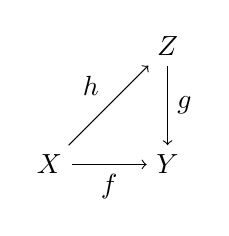
\begin{tikzpicture}
    \node (x) at (0,0) {$X$};
    \node (z) at (1.5,1.5) {$Z$};
    \node (y) at (1.5,0) {$Y$};

    \draw[->] (x) -- (y) node[midway, below] {$f$};
    \draw[->] (z) -- (y) node[midway, right] {$g$};
    \draw[->] (x) -- (z) node[midway, above left] {$h$};
  \end{tikzpicture}
  \caption{A commutative diagram for \cref{def:lift}}
\end{figure}
\begin{conjecture}\label{prop:lift-to-solid-torus}
  A knot $K : S^1 \into \RR^3$ is tame iff there exists an embedding
  $K_{\rm tor} : S^1\times \mbb{D}^2 \into \RR^3$ such that the
  embedding $\iota : S^1 \into S^1 \times \mbb{D}^2$ given by
  \[
    \iota(s) = (s, \mb 0)
  \]
  (where $\mb 0$ is the center of $\mbb{D}^2$)\footnote{Really, any
    point in $\pn{\mbb{D}^2}^\circ$ works.} satisfies $K = K_{\rm
  tor} \circ \iota$.
\end{conjecture}
\begin{figure}[H]
  \centering
  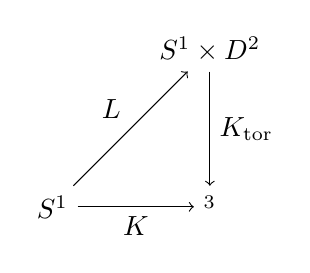
\begin{tikzpicture}
    \node (x) at (0,0) {$S^1$};
    \node (z) at (2,2) {$S^1 \times \mbb{D}^2$};
    \node (y) at (2,0) {$\RR^3$};

    \draw[->] (x) -- (y) node[midway, below] {$K$};
    \draw[->] (x) -- (z) node[midway, above left] {$L$};
    \draw[->] (z) -- (y) node[midway, right] {$K_{\rm tor}$};
  \end{tikzpicture}
  \caption{A commutative diagram for \cref{prop:lift-to-solid-torus}}
\end{figure}
It's worth mentioning that we have recently found a discussion of this
proposition in a MathOverflow post by user \cite{TubularNeighborhood};
however, a proof of the hard portion (existence of $K_{\rm tor}$
implies $K$ tame) was not included. We offer a tentative sketch of a
possible approach, but we offer no guarantees on correctness.
\begin{sproof}[Possible Sketch]
  Let $K : S^1 \into \RR^3$ be an embedding.
  \begin{iffproof}
  \item Suppose $K$ lifts to an embedding $K_{\rm tor} : S^1 \times
    \mbb{D}^2 \into \RR^3$ by the map $\iota : S^1 \into S^1 \times
    \mbb{D}^2$. Note, for all $s \in S^1$, the image $D_s =
    \fim{K_{\rm tor}}{s \times \mbb{D}^2} \subseteq\RR^3$ is
    homeomorphic to $\mbb{D}^2$, hence $\mrm{diam}(D_s) > 0$. Also
    observe that for all $t \in S^1$ with $t \neq s$, $t \not \in
    D_s$.\footnote{Even stronger, $D_t \cap D_s = \varnothing$}

    Show that in a non-trivially knotted region of $K$, the diameters
    $\mrm{diam}(D_s)$ are bounded by the distance between strands
    participating in a crossing. Then, suppose (to obtain a
    contradiction) that $K$ were wild. Show that the distance between
    crossing strands goes to $0$ as we approach the wild point, and
    obtain the contradiction.
  \item For the reverse proof, use the fact that $K$ is tame to obtain
    a homeomorphism $f : \RR^3 \to \RR^3$ such that $\msf K = f \circ
    K$ is polygonal. Construct the tubular neighborhood $N_{\rm tube}$
    of $\fim{\msf K}{S^1}$ using the
    \hyperlink{alg:tubular-neighborhood}{algorithm} described above
    (\cpageref{alg:tubular-neighborhood}). Note, since $f$ is a
    homeomorphism, $\fpre{f}{N_{\rm tube}}$ is homeomorphic to the
    torus $S^1 \times \mbb{D}^2$. Define $K_{\rm tor}$ in terms of
    $\fpre{f}{N_{\rm tube}}$, and show that it satisfies the desired
    properties.\renewcommand{\qedsymbol}{$\boxed{?}$}\qedhere
  \end{iffproof}
\end{sproof}
In any case: While this definition might have some theoretical
properties, it is hard to find a reference for, and seems to be easy
to accidentally misapply if care is not taken to be rigorous (e.g.,
again, we imagine most people employing this definition would guess
that \cref{fig:twists-perspective} is wild at first glance).

\begin{question}
  What does the torus in \cref{fig:twists-perspective} look like?
  We've managed to make some for earlier examples; e.g., an $xy$ plane
  projection of \cref{fig:3d-countable-reidemeister-i-plot} yields a
  picture that looks qualitatively similar to the following, hence we
  can draw a tubular neighborhood without too much trouble:
  \begin{figure}[H]
    \centering
    \includegraphics[scale=.7]{\figdir/smooth-countable-zigzag.pdf}
    \caption{A rough ``flavor'' for what the $xy$-plane projection of
      \cref{fig:3d-countable-reidemeister-i-plot} looks like. Note,
      this is actually a different (nicer-looking) function, but the
      idea is the same.}
  \end{figure}
  We'd be interested in seeing more plots of the associated embedded
  toruses for feral knots.
\end{question}


\section{Common Def. 4}
This section is very short: Given the abundance of examples of tame
knots with countably-many crossings that we have demonstrated, we
discourage the use of Common Definition \hyperlink{def:cdef4b}{4}. We
wonder whether the definition given there was supposed to be ``for
every tame knot $K : S^1 \into \RR^3$, there exists a projection $\pi
: \RR^3 \to \RR^2$ such that $\pi(K)$ has only finitely many
crossings.''

We are skeptical of this claim as well --- it's not obvious what there
is to stop us from taking 6 arcs shaped like the one in
\cref{fig:twists-perspective} and orienting them so that the ``core''
of each of the spirals (formally, the line normal to the plane in
\cref{fig:twists-top} passing through the center of the spiral) lies
along one of the $x,y$, or $z$ axes (each axis gets two spirals, one
pointing in the negative direction, the other pointing in the positive
direction). It seems that no projection of such a knot would yield
only finitely-many crossings, but we'd be willing to be surprised.

\section{Conclusion}
In this chapter, we've introduced several common definitions for
tameness/wildness/local flatness for knots, and established
correspondence (or lack thereof) with the definitions given in
\cite{Daverman}. We also gave a brief discussion of the differences
between the Topological, PL, $C^k$, and $C^\infty$ categories. The
remainder of this document will be concerned with building tools for
working hands-on with ambient isotopy in the Topological category. Our
goal is ultimately to lay the groundwork for characterizing ambient
isotopy between embeddings that can be represented by a countable
union of polygonal segments. To that end, we first turn our attention
to some machinery based in the tools of real analysis.





%%% Local Variables:
%%% TeX-master: "../../kobayashi-thesis"
%%% End:


\chapter{Machinery}\label{chap:machinery}
\setlength\epigraphwidth{.85\textwidth}
\epigraph{``Now stop!'' Max said and sent the wild things off to bed\\
  without their supper. And Max the king of all wild things was lonely\\
  and wanted to be where someone loved him best of all.}{---Maurice
  Sendak, \emph{Where the Wild Things Are}}

In this chapter, we develop two pieces of machinery that are extremely
useful in working with general topological ambient isotopies. The
first is a \emph{uniform convergence} version of
\cref{thm:countable-gluing-ambient-isotopies}, which has the benefit
of not requiring disjointness for our $V_n$. This is a double-edged
sword: On the one hand, it affords us greater latitude in the kinds of
situations where we can apply it, but on the other, it is much easier
to accidentally misuse.

The second is \emph{separation of strands}, which essentially allows
us to partition our knot into segments that are all ``isolated'' from
each other except at their ends (where they share mutual points with
the neighboring strands).\footnote{Note, we will not make any
  guarantees about how complicated the segments themselves look, only
  that they are separated from each other.} This will allow us to work
``locally'' on our knots by keeping our ambient isotopies contained to
regions where they can only affect one part, which will prove
indispensable in the subsequent chapters.




\section{Uniform Convergence and Ambient Isotopy}
% The next theorems will form the backbone of more-or-less all of our
% examination of general topological embeddings.
The following theorems will play a central role in allowing us to
prove all arcs are ambient isotopic in $\RR^2$. The idea is to use
uniform convergence to concatenate countably-many ambient isotopies
together without breaking any of our continuity concerns. We first
recall some definitions from Analysis, then we prove the ambient
isotopy uniform convergence theorem.
\begin{definition}[Uniform Convergence]
  Let $(E,d)$, $(E', d')$ be metric spaces, and for all $n \in \NN$,
  let $f_n : E \to E'$. Also let $f : E \to E'$. Then we say $f_n \to
  f$ \emph{uniformly} iff for all $\varepsilon > 0$, there exists $N
  \in \NN$ such that if $n > N$, then $\forall x \in E$,
  \[
    \abs{f(x) - f_n(x)} < \varepsilon.
  \]
  We will sometimes denote uniform convergence by $f_n \xrightarrow{u}
  f$.
\end{definition}
\begin{proposition}\label{prop:uniform-convergence}
  For all $n \in \NN$, let $f_n : E \to E'$ be a continuous function.
  Now, let $f : E \to E'$, and suppose that $f_n \uconv f$. Then $f$
  is continuous.
\end{proposition}
The proof is an $\frac{\varepsilon}{3}$ argument and can be found in
any standard analysis text.
                        %                         \begin{corollary}
                        %                         Let $E, E', E''$ be compact metric spaces. For all $n \in \NN$, let
                        %                         $f_n : E \to E'$ and $g_n : E' \to E''$ be continuous. Also let $f:
                        %                         E \to E'$ and $g : E' \to E''$, and suppose that $f_n \uconv f$ and
                        %                         $g_n \uconv g$. Then for all $x \in E$,
                        %                         \[
                        %                         \lim_{n\to\infty} (g_n \circ f_n)(x) = (g \circ f)(x).
                        %                         \]
                        %                         \end{corollary}
                        %                         \begin{sproof}
                        %                         Let $\varepsilno$
                        %                         \end{sproof}

\begin{corollary}\label{cor:uniformly-convergent-homeomorphisms}
  Let $(E, d)$, $(E', d')$ be metric spaces, and for all $n \in \NN$,
  let $f_n : E \to E'$ such that $f_n$ is a homeomorphism. Let $f : E
  \to E'$ be a bijection and suppose that
  \begin{enumerate}
    \item $f_n \uconv f$, and
    \item $f^{-1}_n \uconv f^{-1}$
  \end{enumerate}
  Then $f$ is a homeomorphism.
\end{corollary}
\begin{sproof}
  Continuity of $f$, $f^{-1}$ follows directly from
  \cref{prop:uniform-convergence}. Bijectivity gives us a
  homeomorphism.
\end{sproof}

% \begin{question}
%   Is it possible to drop one of (a) bijectivity, or (b) $f_{n}^{-1}
%   \uconv f^{-1}$? In all of the examples we have found where one
%   breaks, the other breaks too. It seems that there should be a
%   straightforward proof using
% \end{question}

% \begin{proposition}
%   Let $f_n : E \to E'$ such that $f_n$ is a homeomorphims. Let $f : E
%   \to E'$ be a bijection, and suppose that $f_n \uconv f$. Then
%   $f_n^{-1} \uconv f^{-1}$.
% \end{proposition}
% \begin{proof}
%   Let $\varepsilon > 0$ be given. Then there exists $N \in \NN$ such
%   that $n > N$ implies that for all $x \in E$, $f_n(x) \in
%   B_\varepsilon(f(x))$.
% \end{proof}
% \begin{sproof}

% \end{sproof}


% \begin{question}
%   Is it possible to drop the bijectivity requirement here, in light of
%   both $f_n \uconv f$ and $f_n^{-1} \uconv f^{-1}$?
% \end{question}
% \begin{remark}
%   It is not possible to drop the bijectivity condition. We'll see an
%   example of why in \cref{ex:fox-artin-curve}.
% \end{remark}


% \subsection{Uniform Convergence and Ambient Isotopy}
We have the following straightforward lemma.
\begin{lemma}\label{lem:countable-homeomorphisms}
  Let $(E,d)$ be a metric space. For all $k\in\NN$, let $V_k \subseteq
  E$, and let $f_k : E \to E$ be a homeomorphism such that $f_k$ is
  identity on $E \setminus V_k$. Define $f : E \to E$ by
  \begin{align*}
    f
    &= \lim_{n\to\infty} \comp_{k=1}^n f_k \\
    &= \lim_{n\to\infty} \pn{f_n \circ f_{n-1} \circ \cdots \circ
      f_{2} \circ f_1}.
  \end{align*}
  Then provided
  \begin{enumerate}
    \item $f$ is a bijection,
    \item The $g^{-1}_n$ defined by $g_n^{-1} = f_1^{-1} \circ \cdots
      \circ f_{n-1}^{-1} \circ f_n^{-1}$, satisfy $g_n^{-1} \uconv
      f^{-1}$, and
    \item The $V_k$ satisfy
      \[
      \lim_{n\to\infty} \mrm{diam}\pn{\bigcup_{k=n}^\infty V_k} = 0,
      \]
  \end{enumerate}
  Then $f$ is a homeomorphism.
\end{lemma}
\begin{remark}
  Note, if $E$ is a compact Hausdorff space, we can drop the condition
  on the $g_n^{-1}$'s, since a continuous bijection from a compact
  space to a Hausdorff space is always a homeomorphism. In particular,
  if $\bigcup_{k=1}^\infty V_k$ is bounded in some compact set, then
  it suffices to prove $f$ is continuous. We stated the more general
  version of the result here, but from now on, we will generally
  assume that we have this simplifying condition.
\end{remark}
\begin{sproof}
  For all $n\in \NN$, define
  \[
    g_n = \comp_{k=1}^n f_k,
  \]
  and note that it is a homeomorphism with inverse
  \begin{align*}
    g^{-1}_n
    &= \comp_{k=1}^n f^{-1}_{n+1-k} \\
    &= f^{-1}_{1} \circ f^{-1}_2 \circ \cdots \circ f^{-1}_{n-1} \circ
      f^{-1}_n.
  \end{align*}
  Since we assume bijectivity of $f$ and $g_n^{-1} \to f^{-1}$ (thus
  $f^{-1}$ is continuous) by hypothesis, it suffices to show that $f$
  is continuous. To that end, we want to show $g_n \uconv f$. Let
  $\varepsilon > 0$ be given. Note that because
  \[
    \lim_{n\to\infty} \mrm{diam}\pn{\bigcup_{k=n}^\infty V_k} = 0,
  \]
  there exists $n_0 \in \NN$ such that $n > n_0$ implies
  \[
    \mrm{diam}\pn{\bigcup_{k=n}^\infty V_k} < \varepsilon.
  \]
  Hence, let $n > n_0$ be fixed, and let $U_n$ denote
  \[
    U_n = \bigcup_{k = n}^\infty V_k
  \]
  Observe that by definition, $f = g_n$ on $E \setminus U_n$, hence
  they are trivially $\varepsilon$-close on $E \setminus U_n$.

  For showing $\varepsilon$-closeness on the $U_n$, note that
  $\fim{f}{U_n} = \fim{g_n}{U_n}$. Thus because $\mrm{diam}(U_n) <
  \varepsilon$, it follows that $f, g_n$ are $\varepsilon$-close on
  $U_n$ as well. Hence $g_n \uconv f$, so $f$ is continuous.

  By \cref{cor:uniformly-convergent-homeomorphisms}, it follows that
  $f$ is a homeomorphism.
\end{sproof}




This extends naturally to the following version for ambient isotopies.
The statement might appear a bit complicated, but it's really just
saying that whenever we're given a collection of ambient isotopies
that are restricted to acting on sets whose radii decay sufficiently
quickly, we can play countably many of them back-to-back in finite
time and yield an ambient isotopy.
\begin{theorem}[Ambient Isotopy and Uniform
  Convergence]\label{thm:uniformly-convergent-ambient-isotopy}
  Let $(E,d)$ be a metric space. For all $k \in \NN$, let $V_k
  \subseteq E$, and let $F_k : [0,1] \times E \to E$ be an ambient
  isotopy such that $F_k$ is identity on $[0,1] \times (E \setminus
  V_k)$. For all such $k$, define $f_k(x) : E \to E$ by $f_k(x) =
  F_k(1, x)$; note that by definition of ambient isotopy, $f_k(x)$ is
  a homeomorphism. Then define $F : [0,1] \times E \to E$ as follows:
  For all $(t,x) \in [0,1] \times E$, let
  \[
    F(t, x) =
    \begin{cases}
      F_1(2t, x) & \text{if } t \in \bk{0, \frac{1}{2}} \\
      F_2(4 (t - 1/2), f_1(x)) & \text{if } t \in \pb{\frac{1}{2},
        \frac{3}{4}} \\
      F_3(8 (t - 3/4), f_2(f_1(x))) & \text{if } t \in
      \pb{\frac{3}{4}, \frac{7}{8}} \\
      \hspace{.5em} \vdots & \\
      F_n\pn{2^n \pn{t - 1 + \frac{1}{2^{n-1}}}, \comp_{k=1}^{n-1}
        f_k(x)} & \text{if } t \in \pb{1 - \frac{1}{2^{n-1}}, 1 -
        \frac{1}{2^n}} \\
      \hspace{.5em} \vdots & \\
      \comp_{k=1}^\infty f_k(x) & \text{if }t = 1.
    \end{cases}
  \]
  Then provided
  \begin{enumerate}
    \item $F(1, \cdot)$ is a bijection,
    \item $\bigcup_{k=1}^\infty V_k$ is bounded in a compact set, and
    \item The $V_k$ satisfy
      \[
      \lim_{n\to\infty} \mrm{diam}\pn{\bigcup_{k=n}^\infty  V_k} = 0,
      \]
  \end{enumerate}
  then $F$ is an ambient isotopy.
\end{theorem}
\begin{proof}
  Note that \np{$\bigcup_{k=1}^\infty V_k$ is bounded in a compact
    set} allows us to apply the simplifying condition for
  \cref{lem:countable-homeomorphisms}.
  \begin{enumerate}
    \item To show $F(0, \cdot)$ is identity: Observe $F(0, x) = F_1(0,
      x) = x$, since $F_1(0,x)$ is an ambient isotopy (and hence
      identity for $t=0$).
    \item To show $F(t, x)$ is a homeomorphism for each $t\in [0, 1)$:
      If $t \neq 1$, then there exists $n \in \NN$ such that $t \in
      \pb{1 - \frac{1}{2^{n-1}}, 1 = \frac{1}{2^n}}$. Hence
      \[
      F(t, x) = F_n\pn{2^n \pn{t - 1 + \frac{1}{2^{n-1}}},
      \comp_{k=1}^{n-1} f_k(x)},
      \]
      which is a finite composition of
      homeomorphisms, and thus a homeomorphism.\footnote{``Finite
      composition of homeomorphisms'' follows because for all $t' \in
      [0,1]$, $F_n(t', x)$ and $\comp_{k=1}^{n-1} f_k(x)$ are both
      homeomorphisms.}
    \item To show that $F(1, \cdot)$ is a homeomorphism: Observe that
      $F(1, \cdot)$ is a bijection, $f_k$ is constant on $E
      \setminus V_k$ for each $k$, and $\lim_{n\to\infty} \mrm{diam}
      \pn{\bigcup_{k=n}^\infty V_k} = 0$. Thus by
      \cref{lem:countable-homeomorphisms}, $F(1, \cdot)$ is a
      homeomorphism.
    \item Finally, to show that $F$ is continuous: Define a sequence
      of ambient isotopies $G_n : [0,1] \times E \to E$ such that
      \[
      G_n(t, x) =
      \begin{cases}
        F_1(2t, x) & \text{if } t \in \bk{0, \frac{1}{2}} \\
        F_2(4 (t - 1/2), f_1(x)) & \text{if } t \in \bk{\frac{1}{2},
          \frac{3}{4}} \\
        F_3(8 (t - 3/4), f_2(f_1(x))) & \text{if } t \in
        \bk{\frac{3}{4}, \frac{7}{8}} \\
        \hspace{.5em} \vdots & \\
        F_n\pn{2^n \pn{t - 1 + \frac{1}{2^{n-1}}}, \comp_{k=1}^{n-1}
          f_k(x)} & \text{if } t\in \bk{1 - \frac{1}{2^{n-1}}, 1 -
          \frac{1}{2^n}} \\
        \comp_{k=1}^n f_k(x) & \text{otherwise.}
      \end{cases}
      \]
      Observe that $G_n$ is a piecewise function whose pieces are each
      continuous. By the gluing lemma, it suffices to show $G_n$ is
      continuous at the points where the pieces meet. This follows by
      observing that for each $k \in \set{1, \ldots, n-1}$, $F_k(1,
      x) = F_{k+1}(0, x)$, and $F_n(1, \comp_{k=1}^{n-1}f_k(x)) = f_n
      \circ \comp_{k=1}^{n-1}f_k(x) = \comp_{k=1}^n f_k(x)$.

      We want to show $G_n \uconv F$. By construction, $G_n(t,x) =
      F(t,x)$ everywhere except perhaps for $(t,x)$ in
      \[
      U_n = \bk{1 - \frac{1}{2^n}, 1 - \frac{1}{2^{n+1}}} \times
      \pn{\bigcup_{k=n}^n V_k}.
      \]
      But observe that for all $(t,x) \in U_n$, we have $G_n(t,x)$,
      $F(t,x) \in U_n$, hence as $n \to \infty$
      \[
      d\pn{G_n(t,x),\ F(t,x)} < \mrm{diam}(U_n) < \varepsilon.
      \]
      It follows that $G_n \uconv F$. By
      \cref{prop:uniform-convergence}, it follows that $F$ is
      continuous.
  \end{enumerate}
  Thus $F$ is an ambient isotopy.
\end{proof}
This is a very powerful technique, and it allows us to prove that all
sorts of wacky curves are secretly ambient isotopic. For instance,
consider the following example:
\begin{example}\label{ex:countable-trefoil-arc}
  The following arc can be unknotted by an ambient isotopy $F : [0,1]
  \times \RR^3 \to \RR^3$ keeping the endpoints fixed.
  \begin{figure}[H]
    \centering
    \includegraphics[scale=.7]{\figdir/countable-trefoil-arc.pdf}
    \caption{A very wild-looking tame arc}
  \end{figure}
  The trick is to define the $V_k$ to be a sequence of nested boxes as
  follows:
  \begin{figure}[H]
    \centering
    \includegraphics[scale=.7]{\figdir/countable-trefoil-arc-boxed.pdf}
  \end{figure}
  The reader should imagine these as properly nested rectangular
  prisms in $\RR^3$. For each of the $V_k$, define an ambient isotopy
  $F_k$ performing the following trick:
  \begin{figure}[H]
    \centering
    \includegraphics[scale=.7]{\figdir/countable-trefoil-arc-boxed-removing-1.pdf}
  \end{figure}
  \begin{figure}[H]
    \centering
    \includegraphics[scale=.7]{\figdir/countable-trefoil-arc-boxed-removing-2.pdf}
  \end{figure}
  \begin{figure}[H]
    \centering
    \includegraphics[scale=.7]{\figdir/countable-trefoil-arc-boxed-removing-3.pdf}
  \end{figure}
  \begin{figure}[H]
    \centering
    \includegraphics[scale=.7]{\figdir/countable-trefoil-arc-boxed-removing-35.pdf}
  \end{figure}
  \begin{figure}[H]
    \centering
    \includegraphics[scale=.7]{\figdir/countable-trefoil-arc-boxed-removing-4.pdf}
  \end{figure}
  \begin{figure}[H]
    \centering
    \includegraphics[scale=.7]{\figdir/countable-trefoil-arc-boxed-removing-5.pdf}
  \end{figure}
  \begin{figure}[H]
    \centering
    \includegraphics[scale=.7]{\figdir/countable-trefoil-arc-boxed-removing-6.pdf}
    \caption{An example $F_n$.}
  \end{figure}
  Observe that we can now apply
  \cref{thm:uniformly-convergent-ambient-isotopy} to show that the arc
  can be untangled in finite time. By contrast, we \emph{cannot} apply
  a similar argument to even a slightly-extended version of this arc:
  \begin{figure}[H]
    \centering
    \includegraphics[scale=.7]{\figdir/countable-trefoil-arc-extended.pdf}
    \caption[A non-example]{A case where we can't define the $V_n$
      such that $\lim_{n\to\infty} \mrm{diam}\pn{\bigcup_n V_n} \neq
      0$}
  \end{figure}
  % {\color{red} \LARGE WHY does this not cause problems for the lemmas
  % in chapter 5???????}
\end{example}
We have to be extremely careful when applying this argument, as it is
very easy to subtly fail the hypotheses without noticing. For
instance:
\begin{example}[Fox-Artin Curve]\label{ex:fox-artin-curve}
  Consider the following arc of \cite{FoxArtin}.
  \begin{figure}[H]
    \centering
    \includegraphics[scale=.2]{\figdir/loops-no-boxes.pdf}
    \caption{A non-example}
    \label{fig:loops-no-boxes}
  \end{figure}
  At first, it might appear reasonable to use
  \cref{thm:uniformly-convergent-ambient-isotopy} to ``undo'' each of
  the loops one-by-one. Certainly, one can define a sequence of boxes
  that satisfy both the \np{$\bigcup_{k=1}^\infty V_k$ is bounded in a
    compact set} and \np{$\lim_{n \to \infty} \bigcup_{n\in\NN} V_n =
    0$} conditions:
  \begin{figure}[H]
    \centering
    \includegraphics[scale=.2]{\figdir/loops-boxed.pdf}
    \caption{Some proposed $V_n$}
    \label{fig:loops-with-boxes}
  \end{figure}
  And indeed, one can find a sequence of ambient isotopies that take
  us arbitrarily close to the unknotted strand. Yet, we can
  \emph{prove} that this is actually a wild arc, using the invariant
  introduced by \cite{FoxArtin}.

  \begin{theorem}[Fox-Artin\footnote{Pronunciation Guide:
      \ipa{"a\textsubarch{5}ti:n}} Tameness
    Invariant] \label{thm:fox-artin-tameness}
    Suppose that $\gamma : [0,1] \into \RR^3$ is tamely embedded. Use
    $\ms S$ to denote the image
    \[
      \ms S = \fim{\gamma}{\bk{0,1}},
    \]
    and let $p = \gamma(0)$. Now, let $\set{V_n}_{n =1}^\infty$ be a
    properly-nested sequence of nested closed sets such that for each
    $n$, $p \in V_n^\circ$, and further
    \[
      \set{p} = \bigcap_{n=1}^\infty V_n.% } \subsetneq \cdots V_n
      % \subsetneq \cdots \subsetneq V_2 \subsetneq V_1.
    \]
    Then there exists $N \in \NN$ such that the homomorphism $i_*$
    \[
      \pi_1(V_N - \ms S) \xrightarrow{i_*} \pi_1(V_1 - \ms S)
    \]
    induced by $i : V_N - \ms S \into V_1 - \ms S$ is
    trivial.\footnote{For those who might not have seen it before:
      Here, $\pi_1$ denotes the fundamental group.}
  \end{theorem}
  We will try to be very thorough in the proof for those who might
  have seen the fundamental group before, but not had a lot of
  experience with it. This will likely strike others as a bit
  overkill. The version in Fox \& Artin's paper is much terser, and
  can be found on page 7.\footnote{In case the page numbering has
    gotten messed up, the paragraph begins with ``To show that $Y$ is
    wildly imbedded [sic] we first develop a necessary condition for
    an imbedding of an arc to be tame.''}
  \begin{proof}
    If $\gamma$ is tame, by definition, there exists a closed set $U
    \subseteq \RR^3$ and a homeomorphism $f : \RR^3 \to \RR^3$ such
    that we have
    \[
      (U, \ms S) \stackrel{\mathclap{f}}{\cong} (\text{3-ball},\
      \text{3-ball diameter}).
    \]
    Without loss of generality, we suppose that for all $n \in \NN$,
    $V_n \subseteq U$. Now, let $p' = f(p)$, $\ms S' = \fim{f}{\ms S}$
    (note this is the diameter), and let let $\pn{V_n'}_{n \in \NN}$
    be given by $V_n' = \fim{f}{V_n}$. Note that since $f$ is a
    homeomorphism, the $V_n'$ satisfy all the properties of the $V_n$.
    In particular, $p' \in {V'_1}^\circ$. Thus there exists
    $\varepsilon > 0$ such that
    \[
      B_\varepsilon(p') \subseteq V'_1.
    \]
    Also not that $\set{p'} = \bigcap_{n=1}^\infty V'_n$ implies that
    for some $N \in \NN$, we have
    \[
      V'_N \subseteq B_\varepsilon(p') \subseteq V'_1
    \]
    and thus
    \begin{equation}\label{eq:three-nested-subsets}
      \np{{V'}_N - \ms S'} \subseteq \np{B_\varepsilon(p') - \ms S'}
      \subseteq \np{{V'}_1  - \ms S'}.
    \end{equation}
    Choose some point $q \in W_N$ to serve as the base point for the
    fundamental groups of the sets in \cref{eq:three-nested-subsets}.
    Then observe that a
    \begin{enumerate}
      \item The inclusion $i : V'_N - S' \into V'_1 - S'$ is trivially
        given by composing $i_1 : V'_N - S' \into B_\varepsilon(p')$
        and $i_2 : B_\varepsilon(p') \into V'_1 - S'$
        \begin{figure}[H]
          \centering
          \begin{tikzpicture}
            \node (a) at (-1.5,0) {$V'_N - \ms S'$};
            \node (b) at (0,-1) {$B_\varepsilon(p')$};
            \node (c) at (1.5, 0) {$V'_1 - S'$};

            \draw[right hook->] (a) -- (c) node[midway, above] {$i$};
            \draw[right hook->] (a) -- (b) node[midway, below left] {$i_1$};
            \draw[right hook->] (b) -- (c) node[midway, below right] {$i_2$};
          \end{tikzpicture}
          \caption{Self-indulgent commutative diagram}
        \end{figure}
      \item $\pi_1(B_\varepsilon(p') - \ms S')$ is trivial (since
        $B_\varepsilon(p') - \ms S'$ is an open ball with a radius
        removed), and hence
      \item The induced map $i_{2,*} : \pi_1(B_\varepsilon(p') - \ms S')
        \into \pi_1(V_1' - \ms S')$ is trivial, and hence because $i_*
        = i_{2,*} \circ i_{1, *}$, $i_*$ is trivial.
        \begin{figure}[H]
          \centering
          \begin{tikzpicture}[scale=1.25]
            \node (a) at (-1.5,0) {$\pi_1(V'_N - \ms S')$};
            \node (b) at (0,-1) {$\pi_1(B_\varepsilon(p'))$};
            \node (c) at (1.5, 0) {$\pi_1(V'_1 - S')$};

            \draw[right hook->] (a) -- (c) node[midway, above] {$i_*$};
            \draw[right hook->] (a) -- (b) node[midway, below left]
            {$i_{*,1}$};
            \draw[right hook->] (b) -- (c) node[midway, below right]
            {$i_{*,2}$};
          \end{tikzpicture}
          \caption{Another self-indulgent commutative diagram}
        \end{figure}
    \end{enumerate}
    Now, since homeomorphism preserves the fundamental group, taking
    $V_N = \fpre{f}{V'_N}$ yields the desired result.
  \end{proof}
  One can verify that the $V_n$'s we drew in
  \cref{fig:loops-with-boxes} don't satisfy this property. What's
  the problem?

  The answer is that we lose bijectivity at $t = 1$ --- not on the
  curve itself, but rather on the ambient space. There's no way to
  undo the curve shown in \cref{fig:loops-with-boxes} without
  dragging infinitely-many points down into the wild point. To
  visualize why, imagine passing a solid torus vertically down
  through the first big loop.
  \begin{figure}[H]
    \centering
    \includegraphics[scale=.25]{\figdir/fox-artin-3d.pdf}
    \caption{A 3D perspective.}
    \label{fig:fox-artin-3d-torus}
  \end{figure}
  Observe that as we remove the first loop, we end up pulling the
  cylinder \emph{through} the second loop. Note, we're going to
  replace the torus with a line so as to make the diagrams easier to
  create. The same argument works either way; we felt the torus was
  more intuitive.
  \begin{figure}[H]
    \centering
    \includegraphics[scale=.25]{\figdir/fox-artin-3d-2.pdf}
    \caption{Pulling out a stitch.}
    \label{fig:fox-artin-pulling-out-a-stitch}
  \end{figure}
  As we iterate this process further, note that the string/torus will
  get dragged further and further downwards until finally converging
  to the wild point. In fact, the same result holds for a torus
  passing through \emph{any} such loop, so performing our proposed
  ambient isotopy would actually collapse infinitely-many points of
  the ambient space down to the wild point. Hence, this approach is no
  good, as it violates bijectivity.\footnote{An alternative argument
    is to show the ``undoing'' maps don't converge uniformly.}
\end{example}
\begin{note}
  While we explicitly drew the torus/line in the figures above, note
  that we're not actually thinking about embedding a torus into
  $\RR^3$. Rather, it's just a helpful visualization to see how the
  ambient space \emph{must} get bent as we perform our proposed
  sequence of ambient isotopies.
\end{note}
\begin{remark}
  One might wonder what would happen if instead we were allowed to
  move the loose end and pull \emph{it} through the stitches
  one-by-one. Note that doing so would require moving said strand
  arbitrarily close to the wild point; hence, it would be lost in the
  limit.
\end{remark}
The preceding two examples are meant to convey that we must proceed
with caution when dealing with
\cref{thm:uniformly-convergent-ambient-isotopy}.
\cref{ex:countable-trefoil-arc} shows that it's easy to take examples
that work and have slight extensions break them.
\cref{thm:uniformly-convergent-ambient-isotopy} shows us that it's
easy to be deceived by our pictures; we must be careful to be very
rigorous when entering the realm of general topological embeddings.

Now, we turn to our second tool: separating strands.

\section{Separating Strands}\label{sec:separating-strands}

\subsection{A Note on Notation in $S^1$}\label{sec:s1-notation}
From now on, we'll often have to work directly with sequences, open
sets, etc.\ in $S^1$. To that end we'll want to have some nice
notational shorthand to avoid having to say things like ``let $s_0,
s_1, s_3\in S^1$ such that, if thought of as an embedded $\RR^2$, we
would encounter $s_1$ before $s_2$ when traveling counterclockwise
around $S^1$ starting at $s_0$ \ldots'' Instead, we'll write this with
symbols.
\begin{itemize}
  \item By $s_0 \sprec s_1 \sprec \cdots \sprec s_n$, we mean that
    we'd encounter $s_0$ before $s_1$ before \ldots before $s_n$
    \emph{before} encountering $s_0$ a second time, if traversing
    around $S^1$ counterclockwise. Note, in displaystyle, $\sprec$
    looks like the following:
    \[
    s_0 \sprec s_1 \sprec \cdots \sprec s_n
    \]
    In analogy with $<$, $\leq$, the $\spreceq$ symbol allows the
    possibility of equality.
  \item By $\spn{s_0, s_1}$, $\sbk{s_0, s_1}$, we mean
    {\small
    \begin{align*}
      \spn{s_0, s_1} &= \set[Big]{s \in S^1 \MID s_0 \sprec s \sprec s_1}
      &
        \sbk{s_0, s_1} &= \set[Big]{s \in S^1 \MID s_0 \spreceq s \spreceq s_1}
    \end{align*}}
    and analogously for $\spb{s_0, s_1}$, $\sbp{s_0, s_1}$. We'll
    denote the topology generated by the $\spn{s_0, s_1}$ as $\tcirc$.
  \item Often, we'll think of $S^1$ as a metric space. We'll denote
    the ``ball of radius epsilon around $s$'' by
    $B_{\varepsilon}^\circlearrowleft(s)$.
  \item In general, we will try to refer to elements of $S^1$ by
    $s,t$, etc., but do note that $t$ is also used for the time
    variable in ambient isotopies.
\end{itemize}
Note, despite the notation above looking evocative of an orientation,
we are not actually thinking about $S^1$ as endowed with one. It just
so happens that in the below, we will often need to think about the
``next'' element of a sequence in $S^1$, but again this will be
detached from thinking of $S^1$ as oriented.









All of the theorems we show below work in $\RR^2$ as well as $\RR^3$,
which we can see by taking $K$ to be restricted to a 2D affine subset
of $\RR^3$.
\begin{proposition}\label{prop:separation}
  Let $K : S^1 \into \RR^3$ be an embedding, and let $I_0 = \sbk{s_0,
    t_0}$ and $I_1 = \sbk{s_1, t_1}$ be disjoint closed arcs of $S^1$.
  For the sake of notational compactness, define $Y_0 = \fim{K}{A_0}$
  and $Y_1 = \fim{K}{A_1}$. Then
  \[
    \inf_{\substack{p_0 \in Y_0 \\ p_1 \in Y_1}} d(p_1, p_2) > 0.
  \]
\end{proposition}
\begin{sproof}
  Since $K$ is an embedding, it is a homeomorphism onto its image.
  Now, since $I_0$, $I_1$ are disjoint compact sets, it follows that
  their images under $K$ are as well. Hence $Y_0, Y_1$ are disjoint
  compact sets. From this point, the claim can be proven by one of the
  following methods:
  \begin{enumerate}
    \item (With Analysis) Let $f : Y_0 \to \RR$ be defined as follows:
      for all $y_0 \in Y_0$, we have
      \[
      f(y_0) = \inf_{y_1 \in Y_1} d(y_0, y_1).
      \]
      Continuity of $f$ follows directly from the triangle inequality.
      Now, since $Y_0$, $Y_1$ are disjoiont, $f(y_0) > 0$ for all
      $y_0 \in Y_0$. Since $Y_0$ is compact, $f$ attains $\inf_{y_0
      \in Y_0} f(y_0)$ on $Y_0$, which yields the desired result.
    \item (With Topology) $\RR^3$ is Hausdorff; apply the fact that
      disjoint compact sets in a Hausdorff space can be separated by
      open sets. After a little finagling the proof should pop out.
      \qedhere
  \end{enumerate}
\end{sproof}
\begin{corollary}\label{cor:works-for-open}
  The same result holds if we replace ``disjoint closed arcs'' in
  \cref{prop:separation} with ``arbitrary sets that have disjoint
  closures.''
\end{corollary}
\begin{sproof}
  The exact same proof as above works. We just chose to state the
  specific case in \cref{prop:separation} first because it's more
  directly intuitive.
  % By ``separated'' we really mean the closures of the two arcs are
  % disjoint. Applying \cref{prop:separation} yields the desired result.
\end{sproof}

% The following proposition more or less states that if we take an
% \emph{arbitrary} collection of disjoint subarcs of $S^1$, then
% It's worth noting that even though we have this separation condition,
% we can still find
% \begin{proposition}\label{prop:inf-sep}
%   Let $K : S^1 \to \RR^3$ be a knot. Let $\set{A_i}_{i \in I}$ be a
%   collection of pairwise disjoint closed arcs of $S^1$, and define
%   $\set{X_i}_{i \in I}$ by $A'_i = K(A_i)$ for all $i \in I$. Finally,
%   let $i_0 \in I$ be arbitrary, and let
%   \[
%     X = \bigcup_{i \neq i_0} X_i.
%   \]
%   Then
%   \[
%     \abs{X_{i_0} \cap \ol{X'}} \leq 2,
%   \]
%   and if $A'_{i_0} \cap \ol{A'} = \varnothing$, then $d(A'_{i_0}, A')
%   > 0$.
% \end{proposition}
% \begin{proof}
%   First we prove $\abs{A_{i_0} \cap \ol{A}}\leq 2$. Observe that
%   because the $A_i$ are all disjoint, we have
%   \[
%     A \cap \bigcup_{i \neq i_0} A_i = 0
%   \]
%   which implies
%   \[
%     \bigcup_{i \neq i_0} A_i \subseteq A_{i_0}^c.
%   \]
%   It follows that
%   \[
%     \ol{\bigcup_{i \neq i_0} A_i} \subseteq \ol{A_{i_0}^c},
%   \]
%   hence $A_{i_0} \cap \ol{A} \subseteq A_{i_0} \cap \ol{A_{i_0}^c} =
%   \partial A_{i_0}$. Noting that $\abs{\partial A_{i_0}} = 2$, we get
%   the desired result.

%   It remains to show that if $A_{i_0} \cap \ol{A} = \varnothing$, then
%   $d(A_{i_0}, A) > 0$. First, note that $\ol{A}$ is closed, and
%   $\ol{A} \subseteq S^1$ implies $\ol{A}$ is bounded {\color{red} in
%     the metric induced by $\RR^n$?}. Now, observe that {\color{red}
%     $S^1$ inherits the Heine-Borel property from $\RR^n$}, so $\ol{A}$
%   is compact. By a similar proof to that of Proposition
%   \ref{prop:separation}, we get $d(A'_{i_0}, A') > 0$.
% \end{proof}
% \begin{remark}
%   (All variables are quantified as above). Note, there could exists
%   infinitely many distinct $i_0 \in I$ such that
%   \[
%     \abs{A'_{i_0} \cap \ol{A'}} \neq 0.
%   \]
%   In particular, consider the following partition of $[0,1]$: for all
%   $n \in \NN$, let $c_n = \frac{1}{n} - \frac{1}{n + 1}$. Then
%   consider the sets $A_{n,m}$ be given by for all $m \in \NN$,
%   \[
%     A_{n,m} = \bk{\frac{1}{n+1} + \frac{c_{n}}{2m + 1},\ \
%       \frac{1}{n+1} + \frac{c_{n}}{2m}}.
%   \]
%   Then if we take the $A_{n,m}$ together with sets of the form
%   \[
%     B_n = \bk{\frac{1}{n+1} + \frac{2}{3} c_n, \frac{1}{n}},
%   \]
%   and mod out by $0 \sim 1$, we see that for $n > 1$, each of the
%   $B_n$ satisfies $B_n \cap \ol{B'_n} = \frac{1}{n}$. We can visualize
%   this as follows:
%   \begin{figure}[H]
%     \centering
%     \includegraphics[scale=.7]{figures/infinite-gauss-sequence/countable-separation.pdf}
%     \caption{Visualization of the sets}
%     \label{fig:countable-sep}
%   \end{figure}
%   Note, we could apply a similar argument to show that we can actually
%   have infinitely many of the $B_n$ intersected on both sides.
% \end{remark}
% \begin{proposition}
%   Suppose that some arc contains
% \end{proposition}

The following theorem essentially says that we can separate strands in
a knot by closed, cone-shaped neighborhoods that only possibly
intersect at endpoints. Note, we'll index almost all variables with
$0$ subscripts to make it easier to refer to the analogues for the
other strand described at the end of the statement.
\begin{theorem}\label{thm:separating-strands}
  Let $K : S^1 \to \RR^3$ be a knot, and let $\sbk{s_0, t_0} \subseteq
  S^1$ with $s_0 \neq t_0$. Then there exists a nonempty, open,
  connected set $U_0 \subseteq \RR^3$ such that
  \begin{enumerate}
    \item $\fim{K}{\spn{s_0, t_0}} \subsetneq U_0$,
    \item $\fim{K}{\sbk{s_0, t_0}} \subseteq \ol{U_0}$, and
    \item $\fim{K}{\sbk{s_0, t_0}^c} \cap \ol{U_0} = \varnothing$.
  \end{enumerate}
  Further, given another disjoint arc $\sbk{s_1, t_1}$, the associated
  $U_1$ satisfies $\ol{U_0} \cap \ol{U_1} = \varnothing$.
\end{theorem}
\begin{proof}
  Use $I_0$ to denote $\sbk{s_0, t_0}$, and let its midpoint be
  denoted $m_0$. We first define a collection of ``nested'' subarcs of
  $I_0$ centered at $m_0$.\footnote{We put ``nested'' in scare quotes
    because we'll actually have uncountably many subarcs in this
    collection, so there's no canonical notion of ``successor'' or
    ``predecessor.''}

  Let $\ell$ be the length of $I_0$. Define $\varepsilon_{0, {\rm
      max}} = \frac{\ell}{2}$, and $E_0 \subseteq \RR$ by
  \[
    E_0 = \pn{0, \varepsilon_{0, \rm max}}.
  \]
  For all $\varepsilon_0 \in E$, let
  \[
    I_{\varepsilon_0} = \bcirc_{\varepsilon_0}(m_0),
  \]
  and observe that for all $\varepsilon_0' < \varepsilon_0$, we have
  \begin{equation}
    I_{\varepsilon_0'} \subsetneq I_{\varepsilon_0} \subsetneq
    I_0. \label{eq:containment}
  \end{equation}
  These are the desired ``nested'' subarcs of $I_0$.\footnote{For some
    intuition, note that as $\varepsilon_0 \incto \varepsilon_{0, \rm
      max}$, we have $I_{\varepsilon_0} \incto I_0$.} Also note that
  taking closures in \cref{eq:containment} preserves all of the
  containments.

  Now: Consider the complement $I_0^c$ in $S^1$, and note that it is
  an open arc of $S^1$. Also note that for all $\varepsilon_0 \in
  E_0$, $I_{\varepsilon} \subsetneq I_0$ implies
  \[
    \ol{I_{\varepsilon_0}} \cap \ol{I_0^c} = \varnothing,
  \]
  hence by \cref{cor:works-for-open}, $\delta_{\varepsilon_0}$ given
  by
  \[
    \delta_{\varepsilon_0} = d(\fim{K}{I_0^c},
    \fim{K}{I_{\varepsilon_0}})
  \]
  satisfies $\delta_{\varepsilon_0} > 0$. We use these
  $\delta_{\varepsilon_0}$'s to construct the desired open
  neighborhood $U_0$.

  For each $\varepsilon \in E$, let $U_{\varepsilon_0} \subseteq
  \RR^3$ be defined by
  \[
    U_{\varepsilon_0} = \set{\bm x \in \RR^3 \MID d(\bm x,
      \overrightarrow{K}(\ol{I_{\varepsilon_0}})) <
      \frac{\delta_{\varepsilon_0}}{3}}.
  \]
  Note that each of these $U_{\varepsilon_0}$ are open and
  nonempty.\footnote{We need the $\frac{1}{3}$ for the $\ol{U_0}\cap
    \ol{U_1} = \varnothing$ claim.} Also note that by definition of
  $\delta_{\varepsilon_0}$, for all $\varepsilon_0 \in E_0$, we have
  \[
    U_{\varepsilon_0} \cap I_0^c = \varnothing.
  \]
  Now, let
  \[
    U_0 = \bigcup_{\varepsilon_0 \in E_0} U_{\varepsilon_0}.
  \]
  Observe that $U_0$ is nonempty, open, and
  connected.\footnote{Connectedness follows from being a union of
    pairwise non-disjoint connected sets.} Also note that
  \begin{enumerate}
    \item $\fim{K}{\spn{s_0, t_0}} \subsetneq U_0$,
    \item $\fim{K}{\sbk{s_0, t_0}} \subsetneq \ol{U_0}$, and
    \item By the distributive property,
      \begin{align*}
        \fim{K}{I_0^c} \cap U_0
        &= \fim{K}{I_0^c} \cap \pn{\bigcup_{\varepsilon_0 \in E_0}
          U_{\varepsilon_0}} \\
        &= \bigcup_{\varepsilon_0 \in E_0} \pn{\fim{K}{I_0^c} \cap
          U_{\varepsilon_0}} \\
        &= \varnothing.
      \end{align*}
      Since $s_0, t_0 \not \in I_0^c$ it follows that $\fim{K}{I_0^c}
      \cap \ol{U_0}= \varnothing$ as well, as desired.
  \end{enumerate}
  This completes the proof of the claimed properties of $U_0$; it
  remains to show that given another arc $I_1 = \sbk{s_1, t_1}$ with
  $I_0 \cap I_1 = \varnothing$, the associated $U_1$ satisfies
  $\ol{U_0} \cap \ol{U_1} = \varnothing$.

  We proceed by contradiction. Suppose that $\ol{U_0} \cap \ol{U_1}
  \neq \varnothing$. We show that the points of intersection must be
  at the ends of the arcs $\fim{K}{I_0}$, $\fim{K}{I_1}$.

  To see this, note that by definition, for all $\varepsilon_0 \in
  E_0$,
  \[
    d(\fim{K}{I_{\varepsilon_0}},\ \fim{K}{I_1}) \geq
    \delta_{\varepsilon_0}.
  \]
  and similarly, for all $\varepsilon_1 \in E_1$,
  \[
    d(\fim{K}{I_{0}},\ \fim{K}{I_{\varepsilon_1}}) \geq
    \delta_{\varepsilon_1}.
  \]
  Because the $U_{\varepsilon_0}, U_{\varepsilon_1}$, were defined in
  in terms of $\frac{\delta_{\varepsilon_i}}{3}$, one can use a simple
  triangle inequality argument to show that for all $\varepsilon_0 \in
  E_0, \varepsilon_1 \in E_1$, we have
  \[
    d(U_{\varepsilon_0}, U_{\varepsilon_1}) > \frac{1}{3}
    \min\set{\delta_{\varepsilon_0}, \delta_{\varepsilon_1}}.
  \]
  It follows that if $d(U_0, U_1) = 0$, this must occur when one of
  the $\delta$'s is $0$ (i.e., $\varepsilon_0 = \varepsilon_{0, {\rm
      max}}$ or $\varepsilon_1 = \varepsilon_{1, {\rm max}}$, and
  hence $I_{\varepsilon_0} = I_0$, $I_{\varepsilon_1} = I_1$). This
  implies $\fim{K}{I_0}$, $\fim{K}{I_1}$ share an endpoint, a
  contradiction (\jiong) --- the arcs were assumed to be disjoint.
  \qedhere
\end{proof}
\begin{figure}[H]
  \centering
  \includegraphics[scale=3]{figures/infinite-gauss-sequence/separation-cor-diagram-cropped.pdf}
  \caption{Example of $V$ and the $V_\varepsilon$}
  \label{fig:v-veps}
\end{figure}
We have a number of remarks to make about this theorem.
\begin{remark}
  Note that in general, as $\varepsilon_0 \incto \varepsilon_{0, \rm
    max}$, we get $\delta_{\varepsilon_0} \decto 0$. Further note that
  $\delta_{\varepsilon_0} : (0, \varepsilon_0) \to \RR$ (viewed as a
  function of $\varepsilon_0$) is continuous and can be continuously
  extended to a compact domain $[0, \varepsilon_{0, \rm max}]$ by
  taking $\delta_{\varepsilon_0}(0) = d\pn{m_0, \ol{A^c}}$ and
  $\delta_{\varepsilon_0}(\varepsilon_{0, \rm max}) = 0$. Hence
  $\delta_{\varepsilon_0}$ is in fact uniformly continuous.
  % It follows that even if $A$ is somewhat pathological (see
  % \cref{fig:everywhere-wild-3}, for instance), we can find a
  % double-sided-cone shaped envelope $U$ such that $A \subseteq U
  % \subseteq V$ such that the width of the cone increases linearly as
  % we go through $S^1$. {\color{red} is the wording here too vague?}
\end{remark}
\begin{remark}
  Note that because we chose to define the $I_{\varepsilon_0}$'s in
  terms of the $m_0$, if the parameterization of $K$ places $K(m_0)$
  closer to one of the endpoints $K(s_0)$ or $K(t_0)$, then we'll get
  a much thinner \& narrower $U_0$ than the one shown in
  \cref{fig:v-veps}. There are ways to change the proof above that
  avoid this issue, but we stuck with this version for simplicity.

  On a similar note, observe that the theorem makes no claims about
  \emph{substrands} of the strand $I_0$ being separated from each
  other. Indeed, $K$ could even be everywhere wild on $I_0$! The point
  is just that we can isolate the behavior of $K$ on $I_0$ from the
  behavior of $K$ on $S^1 \setminus I_0$, provided we keep our
  endpoints fixed.
\end{remark}
% \begin{remark}
%   On that note,
% \end{remark}
We have the following question:
\begin{question}
  Is the $U_0$ defined in \cref{thm:separating-strands} always
  homeomorphic to $\RR^3$?
\end{question}
If we restrict ourselves to the analogous theorem for $\RR^2$, a
``yes'' follows from the \cref{thm:jordan-schoenflies}
(Jordan-Schoenflies; see next section). In $\RR^3$, we don't have such
a result; in particular, we can find pathological objects like the
\emph{Alexander horned sphere} that don't partition our space nicely
into two topological $3$-balls. Is it possible to find a knot for
which the $U_0$ displays this kind of behavior? If not, this would
provide us a nice correspondence with \emph{local flatness}.


% Either way, the $\RR^2$ version gets us a very important theorem. One
% should note that we are \emph{not} guaranteed an analogous theorem in
% $\RR^3$.
% \begin{theorem}\label{thm:countable-convexity}
%   Let $K : S^1 \into \RR^2$ be an embedding, and let $\sbk{s_0, t_0}
%   \subseteq S^1$. Let $U_0$ be the neighborhood guaranteed by
%   \cref{thm:separating-strands}. Then $U_0$ can be written as a
%   countable union of convex sets.
% \end{theorem}
% \begin{sproof}[Sketch]
%   By \cite{Kojman1990Oct}, it suffices to show that neither of the
%   following hold:
%   \begin{enumerate}
%     \item There is a perfect subset\footnote{Recall, a set is perfect
%       if it is closed and has no limit points.} $A \subseteq U_0$ such
%       that for every pair of distinct points $a_0, a_1 \in A$, the
%       convex hull $\ip{a_0, a_1} \not\subseteq A$, or
%     \item There is no such set $A$ as defined above, but there
%       \emph{does} exist a perfect set $B \subseteq U_0$ such that for
%       all distinct $b_0, b_1$, $\ip{b_0, b_1} \subseteq B$, \emph{but}
%       adding a third distinct point $b_2 \in B$ yields $\ip{b_0, b_1,
%       b_2} \not\subseteq U_0$.
%   \end{enumerate}
%   We proceed as follows. Note that $(U_0, \fim{K}{\sbk{s_0, t_0}})
%   \cong (\mbb{D}^2, \text{diameter of $\mbb{D}^2$})$.kkkkkkkkkkkkkkkk
% \end{sproof}


% We have the following conjecture:
% \begin{conjecture}
%   The $U_0$ defined in \cref{thm:separating-strands} is homeomorphic
%   to $\RR^3$.
% \end{conjecture}
% It seems this follows fairly easily from \cref{thm:jordan-schoenflies}
% (Jordan-Schoenflies) in $\RR^2$. In $\RR^3$, the situation is a bit
% less clear, since we


% straightforward in $\RR^2$. In $\RR^3$,
% The importance of this result comes from the following:
% \begin{proposition}
%   Quantify all variables as in \cref{thm:separating-strands} above.
%   Then in $\RR^2$, $U_0$ is homeomorphic to $\RR^2$.
% \end{proposition}
% \begin{sproof}
%   Follows from \cref{thm:jordan-schoenflies}
% \end{sproof}

%%% Local Variables:
%%% TeX-master: "../../kobayashi-thesis"
%%% End:


\chapter{Ambient Isotopy in $\RR^2$}\label{chap:ambient-isotopy-in-r2}
% \setlength\epigraphwidth{.85\textwidth}
% \epigraph{``Now stop!'' Max said and sent the wild things off to bed\\
%   without their supper. And Max the king of all wild things was lonely\\
%   and wanted to be where someone loved him best of all.}{---Maurice
%   Sendak, \emph{Where the Wild Things Are}}

\setlength\epigraphwidth{.7\textwidth}
\epigraph{Then all around from away across the world\\
  he smelled good things to eat\\
  so he gave up being king of where the wild things are.\\
  But the wild things cried, "Oh please don't go --\\
  we'll eat you up --- we love you so!"\\
  And Max said, ``No!''}{---Maurice Sendak, \emph{Where the Wild
    Things Are}}


% To that end, we show that \emph{all} knots in $\RR^2$ are ambient
% isotopic to each other (no PL condition needed). Most sources list
% this as a direct consequence of the Jordan-Schoenflies theorem
% (\cref{thm:jordan-schoenflies}); however, we could not find an
% argument that we found detailed enough to be satisfying. Hence we give
% our own proof. This introduces some of the machinery we'll apply to
% the $\RR^3$ case (particularly some results about the extent to which
% we can isolate strands of a general topological embedding from each
% other), and will also provide an opportunity for us to introduce the
% notion of \emph{feral} points.

%     \emph{Feral points} are points in the image of an embedding $K$ where
%     $K$ is highly ``oscillatory,'' as defined by a local transformation to
%     a polar parameterization of $K$. Feral points represent a sort of
%     ``boundary'' to wildness. Every wild point is a feral point, but not
%     every feral point is a wild point. This explains the confusion with
%     the countable Reidemeister I move example the we alluded to in the
%     preface. There, the point of convergence for the loops was a
%     \emph{feral} point for the diagram, which captures the idea of why it
%     looks ``wild'' at first glance.


We will now examine how ambient isotopy behaves in $\RR^2$. Our main
goal is to show that in $\RR^2$, \emph{all} embeddings are ambient
isotopic. The motivation is to use this result to show that in
$\RR^3$, for two curves $\gamma_1, \gamma_2$ embedded in a compact
neighborhood $V \subseteq \RR^3$ such that $\gamma_1$, $\gamma_2$
share the same endpoints, then if $\gamma_1, \gamma_2$ have no
crossing points in the diagram given by some projection map $\pi$,
then $\gamma_1$, $\gamma_2$ are ambient isotopic by an ambient isotopy
fixing $\partial V$. This will be useful later when we attack the
problem of determining which wild knots can be represented by a
countable union of polygonal segments.

To that end, we must first discuss the extent to which we can separate
distinct strands of a knot by closed neighborhoods. This will allow us
to modify our knots locally by considering ambient isotopies in these
neighborhoods that fix the boundaries. Then, we will be able to apply
\cref{thm:uniformly-convergent-ambient-isotopy} or
\cref{thm:countable-gluing-ambient-isotopies} to combine all of these
into a \emph{single} ambient isotopy achieving our desired effects.


% \section{Some Useful Results}
% To go further in studying arbitrary topological embeddings, we need be
% able to partition our embedded knot into (possibly infinitely-man)
% pieces that we can control the local behavior on. As such, we'll need
% to start incorporating some machinery from Analysis. We'll prove some
% technical results about separating strands, and use these to examine
% the relationship between orientatin-preserving homeomorphism and
% ambient isotopy in $\RR^2$. In particular, we'll see that we can drop
% the PL condition and just treat the two like they're the same thing.
% We expect a similar result holds in $\RR^3$, but due to time
% constraints, we were not able to explore the topic.





% We will make use of this in $\RR^3$ by using it to show that
% if a knot has a $2$D projection with
% that \emph{all} embeddings
% in $K : S^1 \into \RR^2$ are ambient homeomorphic.\footnote{Of course,
%   all $K : S^0 \into \RR^2$ are ambient homeomorphic as well, by a
%   simple translation map.} The second gives us some basic
% characterizations of tameness for $K : S^1 \into \RR^3$.
\section{All Embeddings in $\RR^2$ are Ambient Isotopic}
We begin by recalling the Jordan-Schoenflies
theorem:\footnote{Pronunciation guide: \ipa{ZO\;Rd\~a} and \ipa{"S\o
    :nfli:s}, respectively.}
\begin{theorem}[Jordan-Schoenflies]\label{thm:jordan-schoenflies}
  Let $\gamma : S^1 \to \RR^2$ be a simple closed curve, and let
  $\iota : S^1 \into \RR^2$ be the standard inclusion of $S^1$ as the
  unit circle. Then there exists a homeomorphism $f : \RR^2 \to \RR^2$
  such that $f \circ \gamma = \iota$.
\end{theorem}
Note, ``simple closed curve'' is equivalent to ``embedding.'' We just
chose ``simple closed curve'' to match the language commonly used when
stating the theorem. Anyways, the following is an immediate corollary:
\begin{corollary}[All Embeddings in $\RR^2$ are Ambient
  Homeomorphic.]\label{cor:all-embeddings-in-r2-ambient-homeomorphic}
  Let $K_0, K_1 : S^1 \into \RR^2$. Then $K_0$ and $K_1$ are ambient
  homeomorphic.
\end{corollary}
\begin{sproof}
  By Jordan-Schoenflies, there exist ambient homeomorphisms $f_0, f_1
  : \RR^2 \to \RR^2$ such that $f_0 \circ K_0 = \iota = $ and $f_1 \circ
  K_1 = \iota$. Hence
  \begin{align*}
    (f_1^{-1} \circ f_0) \circ K_0
    &= f_1^{-1} \circ (f_0 \circ K_0) \\
    &= f_1^{-1} \circ \iota \\
    &= f_1^{-1} \circ (f_1 \circ K_1)  \\
    &= K_1. \qedhere
  \end{align*}
\end{sproof}
We now show the main result: In $\RR^2$, ambient
orientation-preserving homeomorphism is equivalent to ambient isotopy.
Again, we know this holds in the PL case, but were unable to find a
proof for the topological case. First, we have the following:
\begin{lemma}\label{lem:polygonal-curves-are-equivalent}
  Let $K_0, K_1 : S^1 \into \RR^2$ be simple polygonal curves. Then
  $K_0, K_1$ are ambient isotopic by some $F : [0,1] \times \RR^2 \to
  \RR^2$ such that for some compact set $V$, $F$ is identity on $[0,1]
  \times (\RR^2 \setminus V^\circ)$.
\end{lemma}
\begin{sproof}
  This follows as a consequence of an argument similar to those given
  in \cref{sec:rigorous-ambient-isotopy}. In particular, see
  \cref{cor:moving-through-simplices}
\end{sproof}
Our goal is to take finer and finer polygonal approximation of $K$,
using \cref{lem:polygonal-curves-are-equivalent} to argue ambient
isotopy with the unit circle, and taking a limit to obtain the result.
There is a problem that we need to be mindful of, though: If we aren't
careful, naively connecting subsequent points together with straight
lines will introduce crossings, which would prevent us from applying
\cref{lem:polygonal-curves-are-equivalent}. Our strategy will be to
use \cref{thm:separating-strands} to separate the strands of our knot
from each other, and then use the lemma below to connect the endpoints
of these strands by an $\varepsilon$-close polygonal approximation.
\begin{lemma}\label{lem:polygonal-path-connected}
  Let $X \subseteq \RR^n$ be open and connected. Then $X$ is
  polygonally path-connected.\footnote{I.e., every two points are
    connected by a finite sequence of line segments.}
\end{lemma}
\begin{proof}
  Let $x_0 \in X$ be arbitrarily chosen. We want to show that $x_0$ is
  polygonally path connected to every other point of $X$. To that end,
  define $C_{\rm poly}$ by
  \[
    C_{\rm poly} = \set{x \in X \MID \text{ there exists a finite
        polygonal path in $X$ from $x_0$ to $x$}}.
  \]
  Note that $C_{\rm poly}$, $C_{\rm poly}^c$ partition $X$. We claim
  $C_{\rm poly}$ is clopen.
  \begin{itemize}
    \item ($C_{\rm poly}$ is open): Let $x_1 \in C_{\rm poly}$ be
      arbitrarily chosen. Then by definition, there exists a polygonal
      path $P_{0,1}$ from $x_0$ to $x_1$. We'll use this later.

      Now, since $X$ is open, there exists $\varepsilon > 0$ such that
      $B_{\varepsilon}(x_1) \subseteq X$. We want to show
      $B_{\varepsilon}(x_1) \subseteq C_{\rm poly}$. To that end, let
      $x_2 \in B_{\varepsilon}(x_1)$ be arbitrary, and bserve that the
      straight line from $x_1$ to $x_2$ is a polygonal path in
      $B_{\varepsilon}(x_1)$ (and hence in $X$ as well). Dxenote it by
      $P_{1,2}$. Then concatenating $P_{0,1}$ and $P_{1,2}$ yields
      another finite polygonal path, hence $x_2 \in C_{\rm poly}$.

      Since $x_2$ was arbitrarily chosen, it follows that
      $B_{\varepsilon}(x_1) \subseteq C_{\rm poly}$, as desired.
    \item ($C_{\rm poly}$ is closed): Here, we want to show $C_{\rm
      poly}^c$ is open. We proceed by contradiction.

      To that end, let $x_1 \in C_{\rm poly}^c$ be
      arbitrarily chosen. Suppose, to obtain a contradiction, that
      $\forall \varepsilon >0$, there exists $x_\varepsilon \in
      B_{\varepsilon}(x_1)$ such that $x_\varepsilon \not\in C_{\rm
      poly}^c$. Then $x_\varepsilon \in C_{\rm poly}$. Thus there
      exists a path $P_{0, \varepsilon}$ from $x_0$ to
      $x_\varepsilon$. We have two subcases.
      \begin{enumerate}
        \item Suppose that the straight line path $P_{\varepsilon, 1}$
          from $x_\varepsilon$ to $x_1$ were contained in $X$. Then
          concatenating $P_{0,\varepsilon}$ and $P_{\varepsilon, 1}$
          would yield a finite polygonal path from $x_0$ to $x_1$,
          \jiong.
        \item Suppose that the straight line path $P_{\varepsilon, 1}$
          from $x_\varepsilon$ to $x_1$ were not contained in $X$.
          Then $B_\varepsilon(x_1) \not\subseteq X$. Since
          $\varepsilon > 0$ was arbitrarily chosen, it follows that
          there exists no $\varepsilon > 0$ such that
          $B_\varepsilon(x_1) \subseteq X$. \jiong, $x_1 \in X$, and
          $X$ is open.
      \end{enumerate}
      In either case we obtain a contradiction. Hence, $C_{\rm
      poly}^c$ is open.
  \end{itemize}
  It follows that $C_{\rm poly}$ is clopen.

  Finally, observe that $C_{\rm poly}$ is nonempty, since for any $x
  \in X$, taking $\varepsilon$ sufficiently small yields $x$ is
  polygonally path connected to any $x' \in B_{\varepsilon}(x)$. The
  result follows.
\end{proof}
\begin{remark}
  Note, we don't make any mention of whether the path above is
  guaranteed to be simple. In fact, we can guarantee this: since our
  path is a finite union of polygonal line segments, it intersects
  itself at most finitely many times (if two segments are fully
  parallel, that case can be treated by taking the union of the two
  and performing the following procedure). When that occurs, take a
  subdivision of the path at the points of intersection and trim out
  the extraneous loops. This gives a simple polygonal path.
\end{remark}


% \begin{lemma}
%   Let $K : S^1 \into \RR^2$ be an arbitrary embedding. Let
%   \[
%     s_1 \sprec s_2 \sprec \cdots \sprec s_n
%   \]
%   be a finite sequence of points in $S^1$. Then for each $k = 1,
%   \ldots, \NN$, there exists $n_k \in \NN$ and points $t_{k, i_n}$ in
%   $S^1$ such that
%   \[
%     s_k \sprec t_{k, 1} \sprec t_{k, 2} \sprec \cdots \sprec
%     t_{k, n_k} \sprec s_{k+1},
%   \]
%   and the polygonal curve formed by linking all of the $K(s_1),
%   K(t_{1,i_1}), \ldots, K(s_n), K(t_{n,i_n}), K(s_1)$ together
%   contains no crossings.
% \end{lemma}
% \begin{proof}
%   Note, since $K$ is a continuous function from a compact space, it
%   follows that $K$ is uniformly continuous.
%   % Note, the $s_k$ partition

%   % If linking our $\pn{K(s_k)}_{k=1}^n$ in order does not create any
%   % crossings, then we're done. Hence suppose that a crossing exists.

%   % Partition
%   % Apply the strand separation

%   % By the Jordan-Schoenflies theorem (\cref{thm:jordan-schoenflies}),
%   % $K$ partitions the plane into regions $B_1, B_2$ with $B_1, B_2
%   % \cong \mbb{D}^2$.
% \end{proof}

% \begin{lemma}
%   Let $K : S^1 \into \RR^3$
% \end{lemma}
The theorem now follows fairly easily.
\begin{theorem}\label{thm:all-ambient-isotopic-in-r2}
  Let $\iota : S^1 \into \RR^2$ be the standard embedding of $S^1$ as
  the unit circle, and let $K : S^1 \into \RR^2$ be arbitrary. Then
  $\iota$, $K$ are ambient isotopic.
\end{theorem}
\begin{sproof}
  We'll construct an ambient isotopy from $\iota$ to $K$ by applying a
  uniform convergence argument \`{a} la
  \cref{thm:uniformly-convergent-ambient-isotopy}. First, select $3$
  distinct points $s_{0}\sprec s_{1} \sprec s_{2} \in S^1$.
  \begin{figure}[H]
    \centering
    \includegraphics{\figdir/points-on-s1.pdf}
    \caption{Example $s_{0}$, $s_{1}$, $s_{2}$}
  \end{figure}
  Apply an ambient isotopy $F_0$ to turn $\iota$ into a triangle with
  these points as the vertices.\footnote{See
    \cref{sec:rigorous-ambient-isotopy} for some inspiration on how to
    define this extremely rigorously.}
  \begin{figure}[H]
    \centering
    \includegraphics[scale=.7]{\figdir/points-on-s1-triangle.pdf}
    \caption{Turning $\iota$ into a triangle. The strange layout is
      just to get the diagram to fit on the page. Note, the dashed
      lines represent the boundary of the original triangle $\triangle
      \iota(s_{0}) \iota(s_{1}) \iota(s_{2})$}
  \end{figure}
  We now define a uniformly convergent sequence of polygonal curves
  converging to our embedding.

  For each $n \in \NN$, let $\varepsilon_n = \frac{1}{2^n}$, and note
  that $\varepsilon_n > 0$. Observe that $K : S^1 \into \RR^2$ is a
  continuous function between metric spaces and $K$ has a compact
  domain. Then by the Heine-Cantor theorem we have that $K$ is
  uniformly continuous, hence there exists $\delta_n > 0$ such that
  for arbitrarily chosen\footnote{The double subscripts here are just
    meant to communicate that ``$s_{0_n}$'' refers to a different
    element for each $n$. Hopefully it's not too confusing.}
  \[
    s_{0_n} \sprec s_{1_n} \sprec \cdots \sprec s_{k_n},
  \]
  provided that \np{for all $i = 1, \ldots, k_n-1$ we have $d(s_{i_n},
    s_{i+1_n}) < \delta_n$}, it follows that \np{for all such $i$ we
    have $d(K(s_{i_n}), K(s_{i+1_n})) < \varepsilon_n$ as well}.

  For each $n \in \NN$, define $P_n$ to be the common refinement of
  the partition defined above with $P_{n-1}$. Observe that $P_n$ gives
  us a collection of closed intervals $\sbk{s_{i_n}, s_{i+1_n}}$ such
  that the interiors are pairwise disjoint; denote these by $I_{i_n}$.
  Observe that by \cref{thm:separating-strands}, there exists an open
  neighborhood $U_{i_n}$ such that $U_{i_n}$ is open, nonempty, and
  connected, and $\fim{K}{I_{i_n}}$ intersects $\ol{U_{i_n}}$ only at
  the end points $K(s_{i_n})$, $K(s_{i+1_n})$. Applying
  \cref{lem:polygonal-path-connected}, we can connect the endpoints by
  a finite polygonal path $P_{i_n,
    i+1_n}$.

  Further, observe that by the construction of $U_{i_n}$, we have
  $d(P_{i_n, i+1_n}, \fim{K}{I_{i_n}}) < \varepsilon_n$. Now, define a
  polygonal embedding $K_n$ by linking together all of the $P_{i_n}$.

  Observe that the result is a simple, closed, polygonal
  curve.\footnote{``Simple'' follows because the $\ol{U_{i_n}}$ are
    all disjoint except perhaps at the endpoints. The endpoints are
    unchanged by applying \cref{lem:polygonal-path-connected}.} By
  \cref{lem:polygonal-curves-are-equivalent}, it follows that all of
  the $K_n$ are ambient isotopic to each other by ambient isotopies
  $F_n : [0,1] \times \RR^2 \to \RR^2$. For each $n= 0,1,\ldots$,
  define $f_n : \RR^2 \to \RR^2$ to be the homeomorphism given by
  $f_n(x) = F_n(1, x)$. Then define an ambient isotopy $F : [0,1]
  \times \RR^2 \to \RR^2$ as follows:
  % \footnote{The $t$ choice of $t$ values might look strange,
  % but }
  \begin{align*}
    F(t, x)
    &=
      \begin{cases}
        F_0\pn{2t, x} & \text{if } t \in \bk{0, \frac{1}{2}} \\
        F_1(4(t - 1/2), f_0(x)) & \text{if } t \in \pb{\frac{1}{2},
          \frac{3}{4}} \\
        F_2(8(t - 3/4), f_1(f_2(x))) & \text{if } t \in
        \pb{\frac{3}{4}, \frac{7}{8}} \\
        \,\cvdots & \\
        F_n\pn{2^{n+1}\pn{t - 1 + \frac{1}{2^n}}, \comp_{k=0}^{n-1}
          f_k(x)} & \text{if } t \in \pb{1 - \frac{1}{2^n}, 1 -
          \frac{1}{2^{n+1}}} \\
        \,\cvdots &
      \end{cases}
  \end{align*}
% \footnote{\label{foot:the-lines}To make this explicit, one
    % can construct the anchor points + lines \`{a} la
    % \cref{sec:rigorous-ambient-isotopy} that would be used for a
    % standard ($\DD^2$, diameter) pair, and then apply the
    % Jordan-Schoenflies theorem to argue that said lines are preserved
    % under the homeomorphism from ($\DD^2$, diameter) to
    % ($\ol{U_{i_n}}, \fim{K}{I_{i_n}}$).}
  After arguing bijectivity, one can then apply a uniform convergence
  argument similar to that in the proof of
  \cref{thm:uniformly-convergent-ambient-isotopy} to the sequence of
  $F_n$'s to show% they are continuous, and
  % similarly to the sequence $\pn{G_n}_{n \in \NN}$ defined by
  % $G_n(x)
  % = F^{-1}(1, x)$ to show it is uniformly convergent to $F^{-1}(1,
  % x)$.
  $F$ is an ambient isotopy. Note that by construction of the $F_n$,
  we have $F(1, \iota(s)) = K(s)$ for all $s \in S^1$. Hence $\iota$
  and $K$ are ambient isotopic, as desired!
  % The following steps will be the key to defining successively closer
  % and closer approximations to $K$. Let $x_{0,0} = f(s_{0,0})$,
  % $x_{0,1} = f(s_{0,1})$, and $x_{0,2} = f(s_{0,2})$. We have three
  % cases. Note, for conciseness, we're going to temporarily use the
  % $\prec$ symbol to denote the relation given by \emph{exactly} $0
  % \prec 1$, $1 \prec 2$, and $2 \prec 0$.\footnote{By ``exactly'' we
  %   mean we don't also say $0 \prec 2$ or $2 \prec 1$ or anything,
  %   just literally only the three pairs given above.} When we say
  % ``for all $i \prec j$,'' we'll take this to mean ``$\forall (i,j)
  % \in \set{(0,1), (1,2), (2,0)}$.''
  % \begin{enumerate}[label=(\roman*)]
  %   \item Suppose the $x_{0, \square}$ are colinear. Observe that since
  %     $K$ does not self-intersect, for all $i \prec j$, there exists
  %     $s_{1,i} \in S^1$ such that
  %     \begin{itemize}
  %       \item $s_{1, i}$
  %       \item
  %     \end{itemize}
  % \end{enumerate}
\end{sproof}
The following is immediate.
\begin{corollary}
  Let $K_0, K_1 : S^1 \into \RR^2$ be arbitrary topological
  embeddings. Then $K_0$ and $K_1$ are ambient isotopic.
\end{corollary}
\begin{sproof}
  $K_0$ and $K_1$ are both ambient isotopic to $\iota$ and ambient
  isotopy is an equivalence relation (just apply one at $2\times$
  speed and then then the inverse of the other also at $2\times$
  speed).
\end{sproof}
Before moving on, it's worth mentioning that a very similar proof to
the above yields the following version for arcs:
\begin{theorem}\label{thm:bounded-arcs-with-same-endpoints}
  Let $\gamma_0, \gamma_1 : [0,1] \into \RR^2$ be embeddings such that
  $\gamma_0(0) = \gamma_1(0)$ and $\gamma_1(0) = \gamma_1(1)$. Also
  let $V \subseteq \RR^2$ be closed such that
  \[
    \partial V \cap \fim{\gamma_0}{[0,1]} = \set{\gamma_0(0),
      \gamma_0(1)} = \partial V \cap \fim{\gamma_1}{[0,1]}
  \]
  Then there exists an ambient isotopy $F : [0,1] \times \RR^2 \to
  \RR^2$ from $\gamma_0$ to $\gamma_1$ such that $F$ is identity on
  $[0,1] \times (\RR^2 - V^\circ)$.
\end{theorem}
In particular, we can locally modify curves in a way that doesn't
affect the rest.
\begin{sproof}[Sketch]
  Use a similar polygonal approximation argument as in the above. To
  get $F$ identity on $[0,1] \times (\RR^2 - V^\circ)$, use the fact
  that $\partial V \cap \fim{K_0}{[0,1]} = \set{K_0(0), K_0(1)} =
  \partial V \cap \fim{K_1}{[0,1]}$ to find appropriate partitions of
  $[0,1]$ such that the approximation gets finer as we approach
  $[0,1]$.
\end{sproof}

% Through similar techniques, one can prove a version of the above that
% allows restricting our ambient isotopies


% Finally, we have the following.
% \begin{corollary}
%   Let $K_0$, $K_1 \into \RR^2$ be embeddings. Then there exists a
%   compact set $V \subseteq \RR^2$ such that $K_0 \cong K_1$ by an
%   ambient isotopy $F : [0,1] \times \RR^2 \to \RR^2$ such that $F$ is
%   identity on $[0,1] \times (\RR^2 \setminus V^\circ)$.
% \end{corollary}
% \begin{sproof}
%   Let $G : [0,1] \times \RR^2 \to \RR^2$ be the ambient isotopy
%   guaranteed by \cref{thm:all-ambient-isotopic-in-r2}. Observe that
%   the function $H : [0,1] \times S^1 \to \RR^2$ defined by
%   \[
%     H(t, s) = G(t, K_0(s))
%   \]
%   is a continuous function with compact domain. Thus $\fim{H}{\bk{0,1}
%   \times S^1}$ is a compact subset of $\RR^2$.
% \end{sproof}

\section{Feral Points}\label{sec:feral-points}
Observe that in \cref{thm:all-ambient-isotopic-in-r2}, we have placed
\emph{no conditions} on $K_0, K_1$ other than that they are
topological embeddings. Hence, even cases like the following example
are covered!
\begin{example}\label{ex:swirly-feral-example}
  Consider a curve defined piecewise by the following dynamics.
  \begin{equation}
    f(r, \theta) =
    \begin{cases}
      \dot{r} = -r^2 \\
      \dot{\theta} = -1.
    \end{cases} \label{eq:polar-form-of-dynamics}
  \end{equation}
  This gives us solutions of the form
  \begin{equation}
    \begin{cases}
      r(t) = \frac{1}{t + \frac{1}{r_0}} \\
      \theta(t) = -t + \theta_0.
    \end{cases} \label{eq:polar-form-of-pathological-curve}
  \end{equation}
  Consider a solution given by $\theta_0 = 0$ and $r_0 > 0$. Then
  converting to Cartesian coordinates by $x(t) = r(t)\cos(\theta(t))$
  and $y(t) = r(t)\sin(\theta(t))$, we have
  \begin{align*}
    \begin{cases}
      x(t) = \frac{\cos\pn{t}}{t + \frac{t}{r_0}} \\
      y(t) = -\frac{\sin\pn{t}}{t + \frac{t}{r_0}}
    \end{cases}
  \end{align*}
  Note, we used $\sin$ odd, $\cos$ even to get the $-$ signs out of
  the arguments. Extend $x(t), y(t)$ to $t = \infty$ by taking
  $x(\infty) = \dot{x}(\infty) = 0$, $y(\infty) = \dot{y}(\infty) =
  0$. As justification: From \cref{eq:polar-form-of-dynamics}, one can
  see that $t = \infty$ gives a fixed point in cartesian coordinates
  (since $\dot{r} = 0$), and by
  \cref{eq:polar-form-of-pathological-curve}, we can see that it
  indeed occurs at $(0,0)$, hence this continuous (and in fact smooth)
  on $\RR^{\geq 0} \cup \set{\infty}$.\footnote{The topology we choose
    on $\RR^{\geq 0} \cup \set{\infty}$ is defined by $U$ is open iff
    $U \in \ms T_{\rm std}$ or $U = V \cup \set{\infty}$ where $V \in
    \ms T_{\rm std}$ is unbounded.} We now have a curve that looks
  something like the following, depending on our choice of
  $r_0$:\footnote{Smaller $r_0$ gives us loops that look more
    circular, since $\dot{r}$ is nonlinear in $r$.}
  \begin{figure}[H]
    \centering
    \includegraphics[scale=.5]{\figdir/plane-spirals-1.pdf}
    \caption{A spiral.}
  \end{figure}
  We want to reparameterize to $\tau \in [0,1]$. Observe that $t :
  [0,1] \to \RR^{\geq 0} \cup \set{\infty}$ given by $\tau(t) =
  \tan\pn{\frac{\pi}{2}t}$ is continuous and monotonic, hence
  \[
    \gamma(\tau) =
    \begin{cases}
      \ms x(\tau) = x(t(\tau)) \\
      \ms y(\tau) = y(t(\tau))
    \end{cases}
  \]
  gives a valid reparameterization of the original trajectory. Now, we
  seek to make $\gamma$ closed. To do so, consider two solutions
  $\gamma_0, \gamma_1$ with slightly different initial radii $r_0,
  r_1$. This gives us something like the following.
  \begin{figure}[H]
    \centering
    \includegraphics[scale=.5]{\figdir/plane-spirals-2.pdf}
    \caption{$\gamma_0$ and $\gamma_1$.}
    \label{fig:two-gammas}
  \end{figure}
  One can use the $\dot{r}$ equation in
  \cref{eq:polar-form-of-dynamics} to argue that $\gamma_0, \gamma_1$
  only intersect at $t = 1$. Now, define $\gamma_{0,1}(t)$ by
  \[
    \gamma_{0,1}(t) =
    \begin{cases}
      \gamma_0(2t) & t \in \bp{0, \frac{1}{2}} \\
      (0,0) & t = \frac{1}{2} \\
      \gamma_1(2-2t) & t \in \pb{\frac{1}{2}, 1}.
    \end{cases}
  \]
  It follows that $\gamma_{0,1}(t)$ is
  continuous.\footnote{Unfortunately, it is not smooth; $\dot x(t),
    \dot y(t)$ oscillate unboundedly. To get a smooth (but less pretty
    looking) curve, one can replace the $\dot{r} = -r^2$ equation with
    $\dot{r} = -r$ to yield a logarithmic spiral, after which the
    construction above gives a smooth curve. If doing this, there are
    a number of ways to close the two open ends together: e.g., one
    could extend the tangent line for the inner curve outwards until
    it's possible to close with the outer curve using a semi-circular
    cap. This would yield a $C^1$ embedding, but not a $C^2$ one.} We
  now extend $\gamma_{0,1}$ to a fully closed curve by giving it a
  $\pi$ rotation plus a translation, and concatenating with the curve
  in \cref{fig:two-gammas}.
  \begin{figure}[H]
    \centering
    \includegraphics[scale=.625]{\figdir/plane-spirals.pdf}
    \caption{A ``Wild-Looking'' Curve in $\RR^2$}
    \label{fig:plane-spirals}
  \end{figure}
  Again: as can be seen from \cref{fig:two-gammas}, one can define
  this curve explicitly by applying a rotation to $\gamma_{0,1}(t)$,
  applying an appropriate shift, and adjusting the time scales to get
  agreement on the two boundary points. From
  \cref{thm:all-ambient-isotopic-in-r2}, it follows that this curve is
  ambient isotopic to the unit circle!
\end{example}
There's something strange going on at the centers of the spirals.
Namely, any line passing through them intersects the boundary of the
curve infinitely many times. For lack of a better name, we'll call
such points \emph{feral} points.\footnote{\emph{Feral} is chosen for
  its meaning as ``having escaped from domestication and become wild''
  (Merriam-Webster,
  \url{https://www.merriam-webster.com/dictionary/feral}). If a name
  for this concept already exists, or if the reader has a better
  suggestion for a name, please contact the author at
  \texttt{fkobayashi@g.hmc.edu}.} We'll draw a distinction here
between \emph{wiggly feral points} and \emph{swirly feral points} in
the definitions below. Note, in $\RR^2$, it might not be immediately
obvious why we would want to think of \emph{wiggly feral points} as
pathological at all, since they seem very easy to control. However, as
we'll see in $\RR^3$, points that look like \emph{swirly feral points}
when we take a projection into $\RR^2$ might turn out to be just
\emph{wiggly feral points} in another.
\begin{definition}[Wiggly Feral Point]\label{def:wiggly-feral}
  Let $K : S^1 \into \RR^2$ be an embedding. Let $s \in S^1$, and let
  $p = K(s)$. Reparameterize $K$ to be in polar form $r_p(t), \theta_p(t)$
  (for $t \in S^1$) such that the pole is at $p$. Then if there exist
  sequences $\pn{s_n}_{n \in \NN}, \pn{t_n}_{n \in \NN}$ such that
  \begin{enumerate}
    \item For all $n \in \NN$, $s_n \sprec t_n \sprec s_{n + 1}$, and
    \item At least one of the following holds:
      \begin{enumerate}
        \item For all $n \in \NN$,
          \[
          r_p(t_n) > \max\set{r_p(s_n), r_p(s_{n+1})},
          \]
          or
        \item For all $n \in \NN$,
          \[
          \theta_p(t_n) > \max\set{\theta_p(s_n), \theta_p(s_{n+1})}.
          \]
      \end{enumerate}
  \end{enumerate}
  Then we call $p$ a \emph{wiggly feral point} (sometimes just
  \emph{wiggly point}) of $K$. We say that $K$ is \emph{wiggly feral}
  or \emph{wiggly} at $p$.
\end{definition}
\begin{remark}
  This definition is meant to encode the idea that the graph of $K$
  ``oscillates'' infinitely often as we approach $p$. Note, this is
  quite different form our example in \cref{fig:plane-spirals}, where
  we actually have $\theta \incto \infty$. By contrast, \emph{wiggly
    feral points} are meant to capture behavior like the following:
  \begin{figure}[H]
    \centering
    \includegraphics[scale=.5]{\figdir/feral-point.pdf}
    \caption[Wiggly Arc]{An arc with a wiggly feral point.}
  \end{figure}
  \begin{figure}[H]
    \centering
    \includegraphics[scale=.5]{\figdir/smooth-countable-zigzag.pdf}
    \caption[Another Wiggly Arc]{A closed curve in $\RR^2$ with a
      wiggly feral point. We've drawn a tubular neighborhood around it
      just for pizzazz.
      % We'll look at this diagram again later when
      % we talk about tubular neighborhoods.
    }
  \end{figure}
  \begin{figure}[H]
    \centering
    \includegraphics[scale=.5]{\figdir/koch-snowflake.pdf}
    \caption[An Everywhere Wiggly Arc]{An everywhere-wiggly arc.
      Essentially every non-self-intersecting fractal is everywhere
      wiggly.}
    \label{fig:everywhere-wiggly}
  \end{figure}
\end{remark}
% \begin{remark}
%   Our definition of wiggly feral does not extend to curves that might
%   \emph{look} wiggly, but actually decay monotonically in both $\theta$.
%   \begin{figure}[H]
%     \centering
%     \includegraphics[scale=.75]{\figdir/wiggly-feral-problem.pdf}
%   \end{figure}
%   % We originally included \np{a condition similar to that on
%   %   $\theta_p(t)$} for $r_p(t)$, however, it appeared to us to be
%   % redundant.
%   % Our definition of wiggly feral appears not to cover situations where
%   % we have
% \end{remark}
% \begin{question}

% \end{question}
% We note some unresolved questions about this definition before
% continuing on to \emph{swirly} feral points.
% \begin{question}
%   Is this the best definition for wiggly feral? Are there cases when
%   we have very poorly-behaved $\theta(t)$ that don't have any local
%   optima but still ``oscillate'' wildly (maybe something not of
%   bounded variation, kind of like the Weirstrass function)?
% \end{question}
The case where $\theta \to \infty$ is covered by \emph{swirly feral
  points}.
\begin{definition}[Swirly Feral Point]\label{def:swirly-feral}
  Let $K : S^1\into \RR^2$ be an embedding. Let $s \in S^1$ be
  arbitrarily chosen, and let $p = K(s)$. Reparameterize $K$ to be in
  polar form $r_p(t), \theta_p(t)$ (for $t \in S^1$) such that the
  pole is at $p$. Then if $\theta_p(t) \to \pm \infty$ as $t \to s$,
  we say $p$ is a \emph{swirly feral point} (sometimes just
  \emph{swirly point}) of $K$. We say $K$ is \emph{swirly feral} or
  sometimes just \emph{swirly} at $p$.
\end{definition}
Sometimes it will be helpful to think of the swirly feral points
without needing to reparameterize. The following proposition gives one
way of doing so.
\begin{proposition}\label{prop:swirly-ferality-and-winding-number}
  Let $K : S^1 \into \RR^2$ be an embedding. Let $s \in S^1$ be
  arbitrarily chosen, and let $p = K(s)$. Consider an arbitrary
  infinite sequence of nested arcs $I_n$:
  \[
    \underbrace{\sbk{s_1, t_1}}_{I_1} \subseteq \underbrace{\sbk{s_2,
        t_2}}_{I_2} \subseteq \cdots \subseteq \underbrace{\sbk{s_n,
        t_n}}_{I_n} \subseteq \cdots.
  \]
  For each $n \in \NN$, define $\gamma_n$ to be the (possibly
  non-simple) curve defined by taking $\fim{K}{I_n}$ and connecting
  $K(s_i)$ and $K(t_i)$ with a straight line. Use $w_n$ to denote the
  winding number of $\gamma_n$ about $p$. Then $p$ is a \emph{swirly
    feral point} of $K$ iff there exists such a sequence of $I_n$'s
  such that
  \[
    \lim_{n \to \infty} w_n = \pm \infty.
  \]
\end{proposition}
\begin{remark}
  One should note that we require \emph{nested} arcs in the
  proposition above. The reason might not be immediately obvious: One
  can imagine a variety of swirly-looking curves that yield
  visually-similar graphs to \cref{fig:plane-spirals} but always
  ``double back'' before $w_n$ can get unbounded (we apologize for the
  lack of diagrams here). Why don't we want to include those? As it
  turns out, they are actually easier to treat, and are really better
  thought of as wiggly feral points.
\end{remark}
% \begin{remark}
%   One might note that both the definitions of \emph{wiggly-feral} and
%   \emph{swirly-feral} are tied to the local behavior of $\theta(t)$
%   close to the pole of some polar coordinate system, but only
%   \emph{wiggly-feral}. Why don't we see
%   similar pathologies in $r(t)$? Ultimately, this is by virtue of
%   continuity of $K$: $r(t)$ can be defined as ``for all $t \in S^1$,
%   $r(t) = d(p, K(t))$.'' Hence all of the bad behavior
% \end{remark}

One might wonder whether feral points have to obey some kind of
discreteness properties. This appears not to be the case, but we have
not investigated the matter in great detail. As a first example, note
that \cref{fig:everywhere-wiggly} is actually \emph{everywhere}
wiggly, hence we certainly can't expect discreteness from wiggly feral
points.\footnote{For an even more pathologically-flavored example, one
  might consider an \emph{Osgood curve}, which can actually have
  positive measure in $\RR^2$.} For swirly-feral points, the situation
is a bit trickier, but we propose the following counterexample to the
claim ``swirly feral points must be topologically discrete.''
\begin{counterexample}
  Let $K$ be defined iteratively from $K_n$ as follows.
  \begin{enumerate}
    \item Let $K_0$ be the spiral embedding from
      \cref{ex:swirly-feral-example}.
      \begin{figure}[H]
        \centering
        \includegraphics[width=5cm]{\figdir/plane-spirals-2.pdf}
        \caption{The spiral, redux}
      \end{figure}
    \item Draw a line through the center of the spiral:
      \begin{figure}[H]
        \centering
        \includegraphics{\figdir/swirly-sequence.pdf}
        \caption{A line through the centers}
      \end{figure}
    \item Define $K_i$ as follows: At each point of intersection $x_i$
      of the line with the spiral, $\fim{K}{S^1}$ locally looks like
      an arc. Hence, remove a small portion from $K$, and replace it
      with a shrunk-down copy of the spiral.\footnote{To guarantee the
      spiral will fit, we can apply \cref{thm:separating-strands}.}
      \begin{figure}[H]
        \centering
        \includegraphics{\figdir/swirly-replace.pdf}
        \caption[Replacement process]{A crude diagram for the
          replacement process. Unfortunately, \texttt{pgfplots}'s
          drawing capabilities gave out on us past the second
          replacment.}
      \end{figure}
      By applying uniform convergence, one can show that the limit of
      the $K_i$ is continuous.
  \end{enumerate}
  This gives an infinite sequence of swirly points converging to
  another swirly point. Hence we see the swirly points are not
  topologically discrete.
\end{counterexample}
We imagine that a similar construction can be used in a fractal-like
construction to yield a curve that is swirly feral on an uncountable
set. We leave some questions for future work:
\begin{question}
  Let $K : S^1 \into \RR^3$. Just how ``not discrete'' can the swirly
  feral points of $K$ be? E.g.,
  \begin{enumerate}[label=\arabic*)]
    \item Can the swirly points of $K$ be perfect?\footnote{Recall,
      perfect means ``closed and has no isolated points.''}
    \item Can the swirly points of $K$ be dense in
      $\fim{K}{S^1}$?
    \item Can the swirly points of $K$ have positive measure in
      $\fim{K}{S^1}$? (Here, we're viewing $S^1$ as $[0,2\pi]/\set{0
      \sim 2\pi}$ inheriting the Lebesgue measure on $[0,1]$).
    \item Can $K$ be swirly almost everywhere?
    \item Can $K$ be everywhere swirly feral?\qedhere
  \end{enumerate}
\end{question}
We have the following conjecture:
\begin{conjecture}
  The answers to the first three above are ``yes,'' ``yes,'' ``yes,''
  ``no,'' and ``no.'' Here's some of our intuition:
  \begin{enumerate}[label=\arabic*)]
    \item This seems fairly straightforward to accomplish by
      constructing a $K$ that maps a Cantor set to swirly feral points
      (e.g., identify the two loose ends of each sub-spiral with the
      endpoints of a Cantor set in $S^1$ and prove the
      correspondence).
    \item Here, one might try a construction that iterates through
      $\set{2\pi t \MID t \in \QQ \cap [0,1]}$ where the radii of our
      inserted sub-spirals decay according to the denominator of
      $t$.\footnote{This is basically Thomae's function but swirly.}
    \item Here, one might try the same argument as in (1) but with the
      Smith-Volterra-Cantor set.
    \item Our intuition is a bit shaky on these last two, but it seems
      that any construction for an ``almost everywhere swirly feral
      embedding'' would require the swirls to get small so quickly
      that in the limit, there's no winding about our points of
      interest. We'd be interested to see an example, though.
    \item If almost everywhere swirly feral fails, then so does
      everywhere swirly feral.
  \end{enumerate}
\end{conjecture}
This concludes our discussion of the 2D case. We now move into 3D,
where all the interesting pathologies lie.

%%% Local Variables:
%%% TeX-master: "../../kobayashi-thesis"
%%% End:


\chapter{Moving into $\RR^3$}\label{chap:moving-into-r3}
\setlength\epigraphwidth{.9\textwidth}
\epigraph{The wild things roared their terrible roars and gnashed their terrible teeth\\
  and rolled their terrible eyes and showed their terrible
  claws}{---Maurice Sendak, \emph{Where the Wild Things Are}}


In this chapter, we partially extend the machinery from the previous
chapter for use in $\RR^3$. The idea is that away from crossing
points, arcs in our diagrams in $\RR^2$ can just be treated with
\cref{thm:bounded-arcs-with-same-endpoints}, and this lifts to an
ambient isotopy in $\RR^3$ that only affects one strand. We will use
this in developing a simple condition on our diagrams that guarantees
we can represent the corresponding embeddings by countable unions of
polygonal segments --- namely, that the set of crossing points are
topologically discrete. In addition to tame arcs, certain classes of
wild arcs (e.g., the Fox-Artin curve in \cref{ex:fox-artin-curve})
will fall into this category. This sets the stage for future work in
which we hope to use \cref{thm:uniformly-convergent-ambient-isotopy}
to show an analogue of Reidemeister's theorem holds. We present a
sketch of how we might plan to attack the problem, however, we have
not confirmed the details. % {\color{blue} !!!!!!!!}

We begin by defining a slightly-relaxed version of regular diagrams,
namely \emph{discrete diagrams}. These are identical to regular
diagrams, except we allow the set of crossing points to be
\emph{discrete} instead of restricting them to be \emph{finite}. Note,
the discreteness condition allows at most countably-many crossings
(\cref{prop:at-most-countable-crossings}).

In \cref{sec:controlling-behavior-away-from-crossings} and
\cref{sec:controlling-behavior-near-crossings}, we then develop the
two pieces of machinery needed to analyze such diagrams.
\cref{sec:controlling-behavior-away-from-crossings} is concerned with
demonstrating that planar isotopy is \emph{always} valid, even without
PL constraints. This allows us to control the behavior of our knots
away from crossings, and the proofs are fairly straightforward in
light of \cref{chap:ambient-isotopy-in-r2}. In
\cref{sec:controlling-behavior-near-crossings}, we do the
complimentary analysis, showing we can control the behavior of our
knots near crossing points; in particular, we can represent every
crossing by two perpendicular line segments.\footnote{Of course, this
  might seem obvious, but a rigorous argument turns out to be highly
  technical given that we are \emph{only} assuming the crossings are
  discrete (and not that our knot is tame).}

Finally, we put these pieces together to yield the promised proof that
a discrete diagram is sufficient to guarantee a representation as a
countable union of polygonal segments. Anyways, the definition.

\begin{definition}[Discrete Diagram]
  Let $K : S^1 \into \RR^3$ be an embedding. Let $\pi : \RR^3 \to
  \RR^2$, and let $D$ be the diagram of $K$ given by $\pi$. Then we
  say $D$ is a \emph{discrete} diagram iff
  \begin{enumerate}
    \item (No multi-crossings): For all $p \in D$,
      $\abs{\fpre{\pi}{p}} \leq 2$
    \item (All crossings are transverse): The diagram is locally
      $X$-shaped at points of crossing, and
    \item (Crossings are discrete): The set $\ms C$ of crossing points
      of $D$ is topologically discrete in $\RR^2$. \qedhere
  \end{enumerate}
\end{definition}
We have the following proposition:
\begin{proposition}\label{prop:at-most-countable-crossings}
  If $D$ is a discrete diagram, then the set of crossing points $\ms
  C$ is at most countable.
\end{proposition}
\begin{sproof}
  $\ms C$ is a subspace of $\RR^2$, which is second-countable. It
  follows $\ms C$ is second-countable. Since a discrete space is
  second-countable iff it is countable, we have the desired result.
\end{sproof}

One might wonder what a \emph{non}-discrete diagram might look like,
and whether it is even possible to obtain one. Indeed we can ---
\emph{everywhere-wild} knots are examples of embeddings for which no
diagram is discrete. We provide an example construction below (imagine
taking the limit as $n \to \infty$), but for more on this subject, one
should reference \cite{Shilepsky} and \cite{Bothe1981}.
\begin{figure}[H]
  \centering
  \includegraphics[scale=.3]{figures/infinite-gauss-sequence/test/test-0.pdf}
  \caption{Step 1 in the construction of an everywhere-wild knot}
\end{figure}
\begin{figure}[H]
  \centering
  \includegraphics[scale=.3]{figures/infinite-gauss-sequence/test/test-1.pdf}
  \caption{Step 2 in the construction of an everywhere-wild knot}
\end{figure}
\begin{figure}[H]
  \centering
  \includegraphics[scale=.5]{figures/infinite-gauss-sequence/test/test-2.pdf}
  \caption{Step 3 in the construction of an everywhere-wild knot}
  \label{fig:everywhere-wild-3}
\end{figure}
% Another example comes from the following, which is similar to the
% construction for the koch snowflake.
% \begin{figure}[H]
%   \centering
%   \includegraphics[scale=.1]{figures/rectifiable-knots/koch-knot-0.pdf}
%   % \caption{Step 1 in the construction of an everywhere-wild knot}
% \end{figure}
% \begin{figure}[H]
%   \centering
%   \includegraphics[scale=.1]{figures/rectifiable-knots/koch-knot-1.pdf}
%   % \caption{Step 2 in the construction of an everywhere-wild knot}
% \end{figure}
% \begin{figure}[H]
%   \centering
%   \includegraphics[scale=.1]{figures/rectifiable-knots/koch-knot-2.pdf}
%   % \caption{Step 3 in the construction of an everywhere-wild knot}
%   % \label{fig:everywhere-wild-3}
% \end{figure}





% \begin{figure}[H]
%   \centering
%   \begin{tikzpicture}[scale=.75]
%     % Define the radii of our nested circles
%     \pgfmathsetmacro{\ra}{2} % Biggest
%     \pgfmathsetmacro{\rb}{3} % Medium
%     \pgfmathsetmacro{\rc}{4} % Small

%     % How much spacing in $x$ to put between the circles
%     % \pgfmathsetmacro{\xsep}{10cm}
%     \begin{scope}
%       \foreach \r/\n in {
%         \ra/.2, \rb/.1, \rc/0
%       }{ % Draw the circles first so that they don't cross
%         % with the arrows
%         \draw ($(0, \r) + (0, \n)$) circle (\r cm);
%         \draw ($(10, \r) + (0, \n)$) circle (\r cm);
%       }

%       \foreach \r/\n/\llab/\rlab in {
%         \ra/.2/$F(K)$ polygonal/$C_D$ is finite,
%         \rb/.1/$F(K)$ rectifiable/$C_D$ is discrete,
%         \rc/0/$F(K)$ is a knot/$C_D$ is disconnected
%       }{
%         % Where to draw the node label
%         \pgfmathsetmacro{\nodey}{2*\r - \ra/2}

%         \node (\r k) at (0, \nodey) {\llab};
%         \node (\r d) at (10, \nodey) {\rlab};

%         \begin{scope}[transform canvas={yshift=.3em}]
%           \draw[-implies, double equal sign distance, shorten
%           <=1mm] (\r k) -- (\r d);
%         \end{scope}

%         \begin{scope}[transform canvas={yshift=-.3em}]
%           \draw[-implies, double equal sign distance, shorten
%           <=1mm] (\r d) -- (\r k);
%         \end{scope}

%         \node[above] () at ($(5, \nodey) + (0,.2)$) {$\exists D \st$};
%         \node[below] () at ($(5, \nodey) - (0,.2)$) {$\exists F \st$};
%       }

%       \foreach \ri/\rii in {\ra/\rb, \rb/\rc}{
%         \draw[-implies, double equal sign distance] (\ri k) -- (\rii k);
%         \draw[-implies, double equal sign distance] (\ri d) -- (\rii d);
%       }
%     \end{scope}
%   \end{tikzpicture}
%   \caption{The relationship between diagrams }
% \end{figure}













\section{Controlling Behavior Away from
  Crossings}\label{sec:controlling-behavior-away-from-crossings}
% \setlength\epigraphwidth{.9\textwidth}
% \epigraph{The wild things roared their terrible roars and gnashed their terrible teeth\\
%   and rolled their terrible eyes and showed their terrible
%   claws}{---Maurice Sendak, \emph{Where the Wild Things Are}}
% {\color{blue} needs patch}
We now prove lemmas that allow us to perform planar isotopies in the
toplogical category. The first says that we can polygonalize our
diagrams away from crossing points.
\begin{lemma}\label{lem:polygonalizing-strands}
  Let $K : S^1\into \RR^3$ be an embedding with diagram $D$ and
  associated projection $\pi$. Let $\sbk{s_0, t_0} \subseteq S^1$ such
  that $A = \fim{K}{\sbk{s_0, t_0}}$ participates in no crossings in
  $D$. Then there exists an ambient isotopy $F : [0,1] \times \RR^3
  \to \RR^3$ taking $A$ to a curve $P$ such that $\fim{\pi}{P}$ is
  polygonal.
\end{lemma}
\begin{sproof}[Sketch]
  Use \cref{thm:separating-strands} to find a closed neighborhood $V
  \subseteq \RR^3$ separating $A$ from other strands (except at the
  endpoints). Use $\fim{\pi}{V}$ to apply
  \cref{thm:bounded-arcs-with-same-endpoints} to the diagram to yield
  an ambient isotopy $G : [0,1] \times \RR^2 \to \RR^2$ yielding the
  desired polygonal curve in $\RR^2$. Without loss of generality,
  suppose that $\pi$ projects onto the $xy$ plane; then we can lift
  $G$ an ambient isotopy in $\RR^3$ by the following:
  \[
    F(t, (x,y,z)) =
    \begin{bmatrix}
      G_x(t, (x,y)) \\
      G_y(t, (x,y)) \\
      z
    \end{bmatrix}
  \]
  Here, $G_x$, $G_y$ denote the $x$ and $y$ components of $G$,
  respectively. That $F$ is an ambient isotopy on $\RR^3$ can be
  argued from the fact that $G$ is on $\RR^2$.
\end{sproof}
\begin{corollary}\label{cor:full-polygonalizing-strands}
  With all variables quantified as above, there exists an ambient
  isotopy $F: [0,1] \times \RR^3 \to \RR^3$ taking $A$ to a curve $P$
  such that $P$ is polygonal in $\RR^3$.
\end{corollary}
Note that this is stronger than the preceding claim, which only
guaranteed $\fim{\pi}{P}$ is polygonal.
\begin{sproof}[Sketch]
  First, apply \cref{lem:polygonalizing-strands}. Because the curve is
  now represented as a \emph{finite} collection of polygonal segments
  $P$, one can argue that it's possible to perturb $\pi$ slightly
  (such that it now includes a portion of the view along the $z$
  direction) without introducing any new crossing points. Applying the
  result again to this new curve yields a result that is polygonal in
  $\RR^3$ (since its $x$, $y$, and $z$ components are now all linear).
\end{sproof}

Now, we can show that given a crossing-less strand in a knot, we can
locally ``straighten it out'' to some extent. The removal of feral
points is important in that it allows us to create a ``nice''
neighborhood of our curve in the below.
% we can replace it with any other strand that has the
% same diagram as long as we don't move the endpoints. This effectively
% means we can have our knot do ``whatever we want'' in the vertical
% direction (the one orthogonal to our plane of projection for the
% diagram).
\begin{proposition}\label{prop:replacing-by-same-endpoints}
  Let $K : S^1 \into \RR^3$ be an embedding with diagram $D$ and
  associated projection $\pi$. Let $\sbk{s_0, t_0} \subseteq S^1$ such
  that $\fim{K}{\sbk{s_0, t_0}}$ does not participate in a crossing in
  $D$. Now, let $\gamma : \sbk{s_0, t_0} \into \RR^3$ be a curve such
  that
  \begin{enumerate}
    \item (Same endpoings in $\RR^3$): $\gamma(s_0) = K(s_0)$ and
      $\gamma(t_0) = K(t_0)$, and also
    \item (Same diagram in $\RR^2$): On all of $\sbk{s_0, t_0}$, $\pi
      \circ \gamma = \pi \circ K$.
  \end{enumerate}
  Then if we define
  \[
    K_\gamma(s) =
    \begin{cases}
      K(s) & s \not \in \sbk{s_0, t_0}\\
      \gamma(s) & s \in \sbk{s_0, t_0},
    \end{cases}
  \]
  then $K \cong K_\gamma$.
\end{proposition}
\begin{proof}
  \begin{figure}[H]
    \centering
    \includegraphics{\figdir/3d-curve-2d-diagram.pdf}
    \caption[Example 2D Diagram]{An example of $A$.}
    \label{fig:example-2d-projection}
  \end{figure}
  Let $A_K = \fim{K}{\sbk{s_0, t_0}}$, and let $A_\gamma =
  \fim{K}{\sbk{s_0, t_0}}$. Also let $C = \fim{\pi}{A_K} =
  \fim{\pi}{A_\gamma}$. Observe that the inverse image
  \[
    M = \fpre{\pi}{C}
  \]
  gives us an embedding of a closed subset $S \subseteq \RR^2$ into
  $\RR^3$:
  \begin{figure}[H]
    \centering
    \begin{subfigure}[t]{.5\linewidth}
      \centering
      \includegraphics{\figdir/3d-curve-shadow-2.pdf}
    \end{subfigure}
    \begin{subfigure}[t]{.5\linewidth}
      \centering
      \includegraphics{\figdir/3d-curve-shadow.pdf}
    \end{subfigure}
    \caption[Example Associated 2-manifold]{An example of the embedded
      $S$ (here shown in {\color{blue} blue}), shown split into two
      halves to make the diagram easier to interpret. Note, viewing
      from the top down yields \cref{fig:example-2d-projection}}
    \label{fig:example-2-manifold}
  \end{figure}
  Now, let $V \subseteq \RR^2$ be the neighborhood guaranteed by
  \cref{thm:separating-strands}. We want to find a way to guarantee
  that $\partial V$ gives us two curves that ``trace'' the shape of
  $C$, instead of kind of ``enveloping'' it (see
  \cref{fig:examples-of-neighborhoods}).
  \begin{figure}[H]
    \centering
    \begin{subfigure}[t]{.5\linewidth}
      \centering
      \includegraphics[scale=.9]{\figdir/3d-curve-2d-diagram-n1.pdf}
      \caption{$\cmark$ Good}
    \end{subfigure}~
    \begin{subfigure}[t]{.5\linewidth}
      \centering
      \includegraphics[scale=.9]{\figdir/3d-curve-2d-diagram-n2.pdf}
      \caption{$\xmark$ Bad}
    \end{subfigure}
    \caption{Examples of good and bad $V$'s.}
    \label{fig:examples-of-neighborhoods}
  \end{figure}
  To that end, one can apply \cref{lem:polygonalizing-strands} to
  yield an ambient isotopy $F_P$ giving a polygonal representation
  $P_K$ of $A_K$, and argue that we can guarantee the existence of
  such a $V$ in that case. Note that by the construction in
  \cref{lem:polygonalizing-strands}, applying $F_P$ also yields a
  polygonal representative $P_\gamma$ of $A_\gamma$. In any case, the
  inverse image of the diagram for $A_K$ gives us a polygonal version
  of \cref{fig:example-2-manifold}, denote it $S_P$. Observe that one
  can now apply \cref{thm:bounded-arcs-with-same-endpoints} to $S_P$
  to yield an ambient isotopy $G : [0,1] \times S_P \to S_P$ taking
  $P_K$ to $P_\gamma$. By using a similar argument to
  \cref{prop:pt-to-barycenter} (\cref{sec:rigorous-ambient-isotopy}),
  one can then extend this to an ambient isotopy $H : [0,1] \times (V
  \times \RR) \to \RR^3$ that fixes $\partial V$.\footnote{In 2D, the
    lines are defined by putting one anchor point in $\partial V$, and
    making the other a point on the diagram for $P_K$. The properties
    we need are maintained when we consider the analogues in $\RR^3$.}
  Finally, defining $F : [0,1] \times \RR^3 \to \RR^3$ by
  \[
    F(t, x) =
    \begin{cases}
      F_P(3t, x) & t \in \bk{0, \frac{1}{3}} \\
      H(3t - 1, F_P(1, x)) & t \in \bk{\frac{1}{3}, \frac{2}{3}} \\
      F_P(3-3t, H(1,F_P(1, x))) & t \in \bk{\frac{2}{3}, 1}
    \end{cases}
  \]
  yields an ambient isotopy taking $A_K$ to $A_\gamma$ while keeping
  the endpoints fixed, and not moving any of the other strands of $K$.
  It follows that $F$ defines an ambient isotopy from $K$ to
  $K_\gamma$.
\end{proof}


% We now use this to show that the requirement ``$A_K$, $A_\gamma$ have
% the same endpoints in $\RR^3$'' is unnecessary, in the following
% sense:
% \begin{proposition}\label{thm:same-region-ambient-isotopic}
%   Let $K_0 : S^1 \into \RR^3$. Then
% \end{proposition}

% \begin{theorem}[Same Diagram $\implies$ Ambient Isotopic]\label{}
%   Let $K_0$, $K_1$ be knots with discrete diagrams. Then if the
%   diagrams are the same, $K_0 \cong K_1$.
% \end{theorem}




% {\color{blue}
% \begin{theorem}
%   Let $K_0$, $K_1$ be knots with diagrams $D_0$, $D_1$. Suppose that
%   the crossings in $D_0$, $D_1$ are topologically discrete in $\RR^2$.
% \end{theorem}}


\section{Controlling Behavior Near
  Crossings}\label{sec:controlling-behavior-near-crossings}
\def\figdir{figures/wild/controlling-crossings}

In the following lemma we show that given any knot $K$ with a discrete
diagram, we can ``straighten out'' the strands near each crossing
$c_i$ in the sense that we can find a cylinder around
$\fpre{\pi}{\set{c_i}}$ which $K$ intersects at only four points. In
particular, we can do this in a way that doesn't move any of the
strands outside of our cylinder.
\begin{theorem}[Cleaning up near crossings]\label{thm:cleaning-up-near-crossings}
  Let $K : S^1 \to \RR^3$ be a knot. Suppose that $K$ admits a
  discrete diagram $D$, and let $c_i$ be an arbitrary crossing of $D$.
  Then there exists \np{$\varepsilon, \nu > 0$ with $\nu <
    \varepsilon$} such that
  % \begin{enumerate}
  %   \item $B_{\varepsilon_i'}(c_i) \subseteq B_{\varepsilon_i}(c_i)$,
  %     and
  %   \item
  there exists an ambient isotopy $F : [0,1] \times \RR^3 \to \RR^3$
  with the following properties:
  \begin{enumerate}[label=(\roman*)]
    \item $F$ is identity outside of $[0,1] \times
      \fpre{\pi}{B_{\varepsilon}(c_i)}$, and
    \item $\abs{F(1, K) \cap \partial \bk{\fpre{\pi}{B_{\nu}(c_i)}}}
      = 4$.
  \end{enumerate}
  % \end{enumerate}
\end{theorem}
\begin{note}
  Observe that the two lines above employ radii for the balls. The
  outer one will serve as a sort of ``buffer zone'' we can push things
  into in case we find some extra strands floating around.
\end{note}
\begin{remark}
  At first it might seem like it'd be sufficient to just shrink the
  radius until we're sufficiently close to the crossing. However, it
  turns out this can fail for cases like the following where a feral
  point occurs at the crossing.
  \begin{figure}[H]
    \centering
    \includegraphics{\figdir/approach-pt.pdf}
    \caption{An example of a crossing and a $B_{\varepsilon}$ where
      $\forall \eta \in (0, \varepsilon)$, $K$ intersects
      $B_{\eta}(c_i)$ more than $4$ times.}
    \label{fig:approach-pt}
  \end{figure}
\end{remark}
\begin{proof}
  By definition of a discrete diagram, $c_i$ is an isolated point of
  the set of crossings, $\ms C$. Hence, there exists $\varepsilon > 0$
  such that $B_{\varepsilon}(c_i) \cap \ms C = \set{c_i}$.

  In general, we can have many arcs of $K$ contained in
  $B_{\varepsilon}(c_i)$; however, the definition of a discrete
  diagram stipulates only \emph{two} such arcs will be involved in the
  crossing itself (see \cref{fig:ex-b-veps}).
  \begin{figure}[H]
    \centering
    \hspace{-1cm}
    \includegraphics[scale=.7]{\figdir/extended-curves-on-circle.pdf}
    \caption{Example of $B_{\varepsilon}(c_i)$. The dashed lines show
      places where the strands poke outside $B_{\varepsilon}(c_i)$.
      Note, if being pedantic, the ball should be technically be
      centered on $c_i$.}
    \label{fig:ex-b-veps} % `example b varepsilon'
  \end{figure}
  % {\color{red} \huge Actually this is a diagram for $B_\eta$.}
  We'll
  take a somewhat funky notation here and use $\overleftarrow{A}$ to
  denote the preimage of the arcs in \cref{fig:ex-b-veps}.
  \[
    \overleftarrow{A} = K(S^1) \cap \fpre{\pi}{B_{\varepsilon}(c_i)}.
  \]
  We can visualize $\overleftarrow{A}$ by something like the
  following:
  \begin{figure}[H]
    \centering
    % \hspace{-2cm}
    \includegraphics[scale=.8]{\figdir/extended-curves-on-sphere.pdf}
    \caption{Example $\protect\overleftarrow{A}$ in $\RR^3$, with a
      3-ball drawn to help communicate that we're no longer in
      $\RR^2$. Note that the dashed lines are \emph{not} included in
      $\protect\overleftarrow{A}$.}
  \end{figure}

  % In general, we \emph{don't} get $\overleftarrow{A}$ bound in a
  % 3-ball of radius $\varepsilon_i$. However, we can always bound
  % $\overleftarrow{A}$ in a cylinder of finite length. As it turns out,
  % this will be an extremely convenient way to complete the proof so
  % we'll do that in a moment. First, a word on notation: In the
  % following we'll use $C_i$ to denote a cylinder in $\RR^3$. This is
  % similar to (but unrelated with) the symbol $\ms C$ we used for the
  % set of all crossings of our diagram; the reader should try not to
  % confuse them.

  Without loss of generality, suppose our projection $\pi$ was onto
  the $xy$ plane. We want to show that $\overleftarrow{A}$ is bounded
  in the $z$ direction. To that end, note that $K$ is a continuous
  function from a compact space, hence it is bounded. This gives us
  $\overleftarrow{A}$ is bounded, hence there exists $r_\varepsilon >
  0$ such that $\overleftarrow{A} \subseteq \ol{B_{\varepsilon}(c_i)}
  \times [-r_\varepsilon, r_\varepsilon] $. Call this cylinder
  $C_\varepsilon$.
  \[
    C_\varepsilon = \ol{B_{\varepsilon}(c_i)} \times [-r, r].
  \]
  \begin{figure}[H]
    \centering
    \includegraphics[scale=.5]{\figdir/extended-curves-r3.pdf}
    \caption{An example drawing for $C_\varepsilon$}
  \end{figure}

  % WLOG, suppose $c_i = (0,0)$ and that $\pi$ was the projection onto
  % the $xy$ plane.\footnote{We do this just so that we can write the
  %   description of the cylinder cleanly. Note, rotations and
  %   translations are ambient isotopies on $\RR^3$, so this causes no
  %   problems.} It follows that $\overleftarrow{A}$ is bounded the
  % closed cylinder $C_i = \ol{B_{\varepsilon_i}(c_i)} \times [-2r,
  % 2r]$.\footnote{We need to take $2r$ in case the strands passes
  %   through $(0,0,0)$ and is one of the points realizing the diameter
  %   $r$.}

  We now have a claim. Essentially, it states that if we look at a
  sub-cylinder $C_\eta$ that's small enough, there are only finitely
  many points where our strands intersect the boundary. This will be
  important when we construct an ambient isotopy to remove them later.
  Note, there is nothing special about using $c_i$ defined in the
  following claim. The same should hold for any point in $\RR^3$.

  \begin{leftbar}

    \noindent \textbf{Claim 1:} There exists $\eta, r_\eta > 0$ such
    that $\eta < \varepsilon$, $r_\eta < r_\varepsilon$, and $C_\eta$
    defined by % and only
    % finitely many arcs of $\overleftarrow{A}$ intersect the cylinder
    \[
      C_\eta = \ol{B_{\eta}(c_i)} \times [-r_\eta, r_\eta].
    \]
    is such that $\partial C_\eta \cap \overleftarrow{A}$ is finite.
    % In particular, $C_\eta$ contains the strands yielding the crossing
    % $c_i$ in our diagram.

    \noindent \textbf{Proof of Claim 1:} We show existence for $\eta$;
    the existence of $r_\eta$ follows similarly.

    % \begin{enumerate}
    %   \item Suppose that the strand goes along
    % \end{enumerate}



    % To argue the part about
    % $C_\eta$ containing the strands from the crossing, observe that
    % \np{the contradiction we derive in the proof below works taking
    % $\varepsilon_1 = \varepsilon_i$ (for the $r'$ argument,
    % analogously $r' = r$)} and argue that the crossing strands
    % aren't a proper subset of $\partial C_i$.

    Suppose, to obtain a contradiction, that no such $\eta$ exists.
    One can show that this requires the strand to oscillate infinitely
    (think wiggly-feral point), per the following sketch: The only
    other way the claim could occur would be if for each $\eta$, there
    were a strand going around part of the circumference of
    $B_\eta(c_i)$. One can show that each such strand has nonzero
    length, and that this causes problems with the fact that there are
    infinitely-many $\eta$ (we'd end up filling a portion of the
    region).

    Let $\eta_0, \eta_1 \in (0, \varepsilon]$ with $\eta_0 \neq
    \eta_1$; without loss of generality suppose $\eta_0 < \eta_1$. By
    hypothesis, infinitely many arcs $\set{A_j}_{j \in J}$ of
    $\overleftarrow{A}$ intersect both of the cylinders.
    \[
      C_{\eta_0} = B_{\varepsilon_0}(c_i) \times [-r_\varepsilon,
      r_\varepsilon] \qquad\qquad \qquad\qquad C_1 = B_{\eta_1}(c_i)
      \times [-r_\varepsilon, r_\varepsilon].
    \]
    This might look something like the following:
    \begin{figure}[H]
      \centering
      \begin{subfigure}[t]{.49\linewidth}
        \centering
        \includegraphics[scale=.5]{\figdir/countably-intersecting-cylinder.pdf}
      \end{subfigure}~
      \begin{subfigure}[t]{.49\linewidth}
        \centering
        \includegraphics[scale=.6]{\figdir/countably-intersecting-cylinder-td.pdf}
      \end{subfigure}
      \caption{An example visualization in 3D showing the top strand
        of the crossing, another arc, and the bottom strand of the
        crossing, each separated vertically. The projection obtained
        is shown at the bottom, and the corresponding top-down view
        displayed on the right.}
      \label{fig:example-3d-oscillation-visual}
    \end{figure}
    We want to show this breaks continuity of $K$. To that end, we'll
    employ sequential continuity. First, we define a collection of
    sub-strands that live in the annulus between $\eta_0$ and $\eta_1$:
    For all $j\in J$, let
    \[
      B_j =
      \begin{cases}
        A_j \cap \ol{C_{\eta_1} - C_{\eta_0}} & \text{if } \abs{A_j
          \cap C_{\eta_0}} = 1 = \abs{A_j \cap C_{\eta_1}}, \text{ and }\\
        \varnothing & \text{otherwise}.
      \end{cases}
    \]
    Note that the $B_j$ omit the arcs that just oscillate around one of
    $\partial C_{\eta_0}$, $\partial C_{\eta_1}$ without ever going over
    to the other.

    To ensure the $B_j$ are actually valid arcs, we must subdivide them
    into their maximal connected components and remove all of the empty
    entries. Reindex the $B_j$ accordingly to yield $\set{B_\ell}_{\ell
      \in L}$. Then define sets $\set{O_\ell}_{\ell \in L}$,
    $\set{I_\ell}_{\ell \in L}$ ($O$ for ``outer'', $I$ for ``inner'')
    by for all $\ell \in L$,
    \[
      O_\ell = B_\ell \cap \partial C_{\eta_1}
      \qquad\qquad\text{and}\qquad\qquad I_\ell = B_\ell \cap \partial
      C_{\eta_0}.
    \]
    Let $\pn{O_{n}}{n \in \NN}$ be an arbitrary sequence of distinct
    $O_{\ell}$'s. Note that $C_{\eta_1}$ is compact, thus we can apply
    Bolzano-Weierstrass to $\set{O_{n}}_{n \in \NN}$ to obtain a
    convergent subsequence $\set{O_{n_k}}_{k \in \NN}$. Now, observe
    that because the $O$'s are endpoints of arcs bridging $\partial
    C_{\eta_0}$, $C_{\eta_1}$, each $O_{n_k}$ has a corresponding
    $I_{n_k} \in \partial C_{\eta_0}$. Apply Bolzano-Weierstrass to
    $\set{I_{n_k}}_{k \in \NN}$ to get \emph{another} convergent
    subsequence, call it $\pn{I_{n_m}}_{m \in \NN}$. Note that
    restricting the $O$'s to $\pn{O_{n_m}}_{m \in\NN}$ still yields a
    convergent sequence.

    Now, recall that because $K$ is an embedding, it is a homeomorphism
    onto its image. Thus, image and preimage under $K$ preserve
    convergence, and so taking the elementwise inverse of the $O_{n_m}$,
    $I_{n_m}$ gives us sequences in
    \[
      \set{\ms O_{n_m}}_{m \in \NN} \qquad\qquad \text{and} \qquad\qquad
      \set{\ms I_{n_m}}_{m \in \NN}
    \]
    in $S^1$. One can show that they must converge to the same $s \in
    S^1$ as follows: Observe each arc $A_{n_m}$ linking $O_{n_m}$,
    $I_{n_m}$ corresponds to an interval of one of the forms
    \[
      \sbk{\ms I_{n_m}, \ms O_{n_m}} \qquad\qquad\text{or}\qquad\qquad
      \sbk{\ms O_{n_m}}, \ms I_{n_m}.
    \]
    Since $S^1$ is compact, in order for these intervals to be disjoint
    (required since the images are disjoint) the lengths must go to $0$
    as $m \to \infty$. Thus $\ms O_{\ell_m} \to \ms I_{\ell_m}$.

    But note, taking the image once more gets us that $K(\ms O_{\ell_m})
    = O_{\ell_m} \not \to I_{\ell_m} = K(\ms I_{\ell_m})$ (since the
    $O_{\ell_m}$, $I_{\ell_m}$ are separated by $\eta_1 - \eta_0$). But
    this is a contradiction (\jiong), $K$ preserves convergence. Thus,
    there must exist $\eta > 0$ such that only finitely many of the arcs
    of $\overleftarrow{A}$ intersect $B_\eta(c_i) \times \RR$. Applying
    a similar argument for $r_\eta$ gives us the existence of the
    desired $C_\eta$, which proves the claim. \hfill $\square$

  \end{leftbar}
  % \hrulefill
  \begin{figure}[H]
    \centering
    \includegraphics[scale=.5]{\figdir/extended-curves-r3-two-cylinders.pdf}
    \caption{An attempted drawing of $C_\varepsilon$ and $C_\eta$.
      % Unfortunately, the opacity stacking didn't quite work out, so
      % some portions of the ball / strands got occluded when they
      % shouldn't have been.
    }
    \label{fig:the-cylinders}
  \end{figure}
  \begin{remark}
    Note that in the particular example shown in
    \cref{fig:the-cylinders}, we could have just taken $\eta =
    \varepsilon$. An example of when we can't is when one of the
    strands travels in a circular arc partway around $\partial
    C_\varepsilon$.
  \end{remark}


  OK: By the claim, there exists $\eta$, $r_\eta > 0$ such that
  \[
    \eta \in (0, \varepsilon) \qquad\qquad \text{and} \qquad\qquad
    r_\eta \in (0,r_\varepsilon)
  \]
  and $\overleftarrow{A}$ intersects $\partial C_\eta = B_{\eta}(c_i)
  \times [r_\eta, r_\eta]$ at finitely-many points. Apply the claim a
  second time to define a proper sub-cylinder $C_\nu$ by $C_\nu =
  B_{\nu}(c_i) \times [-r_\nu, r_\nu]$ (where $\nu < \eta$ $r_\nu <
  r_\eta$) such that $\overleftarrow{A}$ only intersects $C_\nu$ at
  finitely-many points.


  The next claim essentially states that we can remove \np{the strands
    that don't participate in our crossing} from $C_\nu$ by pushing
  them out into $C_\eta$. Note, the fact that we have only
  \emph{finitely} many points of intersection helps in avoiding an
  appeal to
  \cref{thm:uniformly-convergent-ambient-isotopy}.\footnote{There is a
    more direct proof using the techniques of
    \cref{sec:rigorous-ambient-isotopy}, but it's horrible to write
    out formally.}

  % {\color{red} \Large Wait there's some more stuff to consider. The
  %   proof I gave was for oscillatory behavior, but that might not be
  %   where the problems lie. Really it's in the garbage w' having
  %   circumference strands??????????????/}

  % an
  % appeal to \cref{thm:uniformly-convergent-ambient-isotopy} (uniform
  % convergence \& ambient isotopy).

  \begin{leftbar}
    \textbf{Claim 2:} Let $S_o, S_u$ be the strands corresponding to
    the overstrand and understrand (respectively) in
    \cref{fig:ex-b-veps}. Let $\set{S_j}_{j =1}^{n}$ be the collection
    of arcs of $\overleftarrow{A}$ that intersect $C_\eta$ but
    \emph{do not} participate in the crossing. Then we can find an
    ambient isotopy $F : [0,1] \times C_\eta \to C_\eta$ such that
    \begin{enumerate}
      \item $F$ keeps \np{both the boundary of $C_\eta$
        \emph{and} the crossing strands $S_o$, $S_u$} fixed, and
      \item For all $x \in S_j$, $F(1, x) \in C_\eta \setminus
        C_\nu$ ($F$ moves all the other strands outside $C_\nu$).
    \end{enumerate}

    \textbf{Proof of Claim 2:} Observe that for each $j=1,\ldots, n$,
    $\partial T_j$ yields a crossing-less curve. Thus, one can apply
    \cref{prop:replacing-by-same-endpoints} to find ambient isotopies
    moving each into $C_\eta \setminus C_\nu^\circ$, keeping the rest
    of the region fixed. Since we have only finitely-many strands to
    remove, concatenating them yields another ambient isotopy. \hfill
    $\square$
    % Consider the following ambient isotopy on $\RR^2$: each of the
    % $M_\mu$ gets sent to the corresponding part of the circumference
    % bordered by $R_\mu$, and each of the displayed portions of the
    % circumference get sent to the \emph{dotted} lines shown. Finally,
    % the rest of the ambient space we're displacing gets squished into
    % the region bounded by the dashed lines, which stay fixed (as do
    % the crossing strands themselves).
    % \footnote{This can be justified
      % by applying \cref{thm:same-region-ambient-isotopic} to each of
      % the finitely-many strands on }


  \end{leftbar}

  One way to visualize the net effect of this process is as follows.
  Note that the crossing strands (marked with the black dots in
  \cref{fig:part-disjoint-regions}) partition $B_{\eta}(c_i)$ into
  four disjoint regions $R_1, R_2, R_3, R_4$ that contact $\partial
  B_{\nu}(c_i)$. Let $M_1, M_2, M_3, M_4$ be defined by for each index
  $\mu \in \set{1,2,3,4}$, $M_\mu = \partial R_\mu$.

  \textbf{Note:} In the figures below, we accidentally re-drew
  $B_\nu(c_i)$ as $B_\varepsilon(c_i)$, and $B_\eta(c_i)$ as some ball
  containing $B_\varepsilon$. We apologize for this inconsistency;
  unfortunately, we currently do not have enough time to go back and
  fix them.
  \begin{figure}[H]
    \centering
    \includegraphics{\figdir/extended-curves-on-circle-partition.pdf}
    \caption{The regions $R_1, R_2, R_3, R_4$, and (approximations
      of) the corresponding $M_1, M_2, M_3, M_4$'s in black. Not to
      scale.}
    \label{fig:part-disjoint-regions}
  \end{figure}
  Then we ``push'' $\partial R_\mu \cap \partial \ol{B_\nu(c_i)}$
  outwards to the dotted curves shown below, and $\partial R_\mu \cap
  B_\nu(c_i)$ out to the circumference. The dashed lines (representing
  $\partial B_\eta(c_i)$) remain fixed.
  \begin{figure}[H]
    \centering
    \includegraphics[scale=.9]{\figdir/extended-curves-on-circle-ms-isotopy.pdf}
  \end{figure}
  Finally: observe that by construction,
  \begin{enumerate}
    \item $C_\nu \subsetneq C_\eta \subsetneq C_\varepsilon$,
    \item $\abs{F(1, K) \cap \partial\bk{\fpre{\pi}{B_\nu(c_i)}}} =
      \abs{F(1,K) \cap \partial C_\nu} = \abs{\set{\text{endpoints of
      $S_o, S_u$}}} = 4$, and
    \item $\partial C_\varepsilon$ remains fixed.
  \end{enumerate}
  As desired.
\end{proof}
\begin{corollary}[$K$ can be polygonalized near crossings]
  Let $K$, $c_i$, $C_\nu$, $C_\varepsilon$ be as defined in the
  preceding theorem/proof. Then there exists an ambient isotopy $F :
  [0,1] \times \RR^3 \to \RR^3$ such that
  \begin{enumerate}
    \item $F$ is identity outside of $[0,1] \times C_\varepsilon$, and
    \item $F(1, K) \cap C_\varepsilon$ is polygonal.
  \end{enumerate}
\end{corollary}
\begin{sproof}[Sketch]
  By the \cref{thm:cleaning-up-near-crossings}, we can find an ambient
  isotopy removing all non-crossing strands from $C_\nu$ while keeping
  $\partial C_\varepsilon$ and \np{the crossing strands themselves}
  fixed. Apply this ambient isotopy from $t = 0$ to $t= 1/2$. Then,
  \begin{itemize}
    \item Observe that there are no other strands in $\fpre{\pi}{B_\nu(c_i)}$
      ``above'' $S_o$ or ``below'' $S_u$.
    \item Use this to define an ambient isotopy flattening out $S_o$
      in the $z$ direction (so that it's only non-polygonal in $x$ and
      $y$), while translating it half of the way to the top circular
      cap of $C_\nu$. Apply a similar ambient isotopy flattening $S_u$
      out in $z$ and moving it half of the way to the bottom circular
      cap.\footnote{Although drawn for a different purpose,
      \cref{fig:example-3d-oscillation-visual} displays this idea
      nicely the blue/red circles. Note, there we drew the crossing
      strands as straight lines in $xy$ as well as in $z$; we have not
      done this yet in our construction.}
    \item Use a proof similar to that of
      \cref{prop:replacing-by-same-endpoints} (taking a smaller
      sub-cylinder if necessary) to turn the crossing strands into
      straight lines while keeping $\partial C_\nu$ fixed.
  \end{itemize}
  This yields the desired result.
\end{sproof}
Finally, this concludes the analysis of behavior near crossing points.
We are now ready to put it all together.

\section{The Conclusion}

Together, these give us the following theorem:
\begin{theorem}[Discrete Diagram Implies Countably
  Polygonal]\label{thm:discrete-diagram-countably-polygonal}
  Let $K : S^1 \into \RR^3$ be a knot. Then if $K$ admits a discrete
  diagram $D$, then $K$ is ambient isotopic to a knot comprised of (at
  most) a countable union of polygonal segments.
\end{theorem}
\begin{proof}
  Apply \cref{thm:cleaning-up-near-crossings} to triangulate $K$ at
  each of the crossing points. Note that this implicitly defines a
  collection of pairwise-disjoint arcs connecting each of the
  resulting $C_\nu$ together. Applying
  \cref{cor:full-polygonalizing-strands}, we can polygonalize each of
  these connecting strands with a finite collection of line segments.

  Finally, observe that for each crossing, this gives us a finite
  collection of corresponding polygonal segments. By
  \cref{prop:at-most-countable-crossings}, we have at most
  countably-many crossings in the diagram, hence the total number of
  polygonal segments employed is at most countable!
\end{proof}
The following appears to be a reasonable extension of the claim.
\begin{conjecture}
  If the set of wild points are topologically discrete, then the same
  result as above holds.
\end{conjecture}
% \begin{sproof}
%   $\msf{K}{S^1}$ is compact, hence a discrete subset
% \end{sproof}

% A couple of other results also follow from patching together parts of
% the arguments above:
The techniques above can be used to obtain a variety of other expected
results. E.g.,
\begin{proposition}
  Let $K_0, K_1 : S^1 \into \RR^3$. Suppose that the diagrams for
  $K_0$, $K_1$ are related by planar isotopy. Then $K_0 \cong K_1$.
\end{proposition}
In particular:
\begin{corollary}
  Let $K_0, K_1 : S^1\into \RR^3$ such that $K_0$, $K_1$ share the
  same discrete diagram $D$. Then $K_0 \cong K_1$.
\end{corollary}
We conclude this section with a discussion of directions for future
work.


\subsection{A Generalization of Reidemeister's Theorem?}
The usual proof of Reidemeister's theorem relies on using
polygonalizations to reduce the problem of ambient isotopy to the
elementary moves. Now that we have a locally-polygonal representation
for some wild knots, can we prove an analogous theorem for countable
sequences of moves? E.g., something like
\begin{conjecture}
  Let $K_0, K_1 : S^1 \into \RR^3$ be knots with discrete diagrams.
  Suppose that $K_0 \cong K_1$. Then there exists a sequence of
  Reidemeister moves satisfying the hypotheses of
  \cref{thm:uniformly-convergent-ambient-isotopy} taking $K_0$ to
  $K_1$.
\end{conjecture}
One plan of attack might be as follows:
\begin{enumerate}
  \item \cref{thm:uniformly-convergent-ambient-isotopy} (or
    alternatively, \cref{thm:countable-gluing-ambient-isotopies})
    gives us an ``if'' direction (provided we're careful to mind
    bijectivity in the
    \cref{thm:uniformly-convergent-ambient-isotopy} case). Hence,
    the main plan of attack would be to find an only-if proof.
  \item One idea could be as follows: First, show that given an
    ambient isotopy $F : [0,1] \times \RR^3 \to \RR^3$ taking
    $K_0$ to $K_1$, we can realize the same effects on $K_0$,
    $K_1$ by restricting $F$ to a compact subspace $V$. Then use
    this to argue that $F$ restricted to $F : [0,1] \times V \to
    V$ is uniformly continuous. Hence, we can partition $[0,1]
    \times V$ into a finite collection of small sub-regions such
    that $F$ is guaranteed to vary by less than $\varepsilon$ on
    them.
  \item First, note that the local sets we constructed in the
    proof in the previous section (e.g., the $C_\nu$, or the sets
    guaranteed by \cref{thm:separating-strands}) can be made
    arbitrarily small. Use this to argue that our choices of
    polygonal representatives can be made continuously dependent
    in some sense on the input knots themselves.
  \item Then, show that in light of the above, away from wild
    points, we can realize the effects of the ambient isotopy
    by local polygonal moves. Near the wild points, keep the
    effect of the given $F$.
  \item Define a uniformly convergent sequence of ambient
    isotopies ``shrinking'' the region where we keep the effects
    of $F$ down to the wild points. Finally, apply
    \cref{thm:uniformly-convergent-ambient-isotopy} to yield the
    result.
\end{enumerate}




% \begin{sproof}

% \end{sproof}

% We have a couple of remarks:
% \begin{remark}
%   Observe that all of the sets we employed ($B_\varepsilon(c_i)$, the
%   $V$'s from \cref{thm:separating-strands}, etc) can all be made
%   arbitrarily small, which allows us to make our polygonalization
%   ``continuously'' dependent on the input knot in some sense.
% \end{remark}
% \begin{remark}
%   By applying \cref{thm:discrete-diagram-countably-polygonal}, one can
%   argue that
% \end{remark}


% \begin{proposition}

% \end{proposition}









%%% Local Variables:
%%% TeX-master: "../../kobayashi-thesis"
%%% End:


\chapter{Conclusion \& Directions for a Category}\label{chap:summary}
\setlength\epigraphwidth{.7\textwidth}
\epigraph{
  but Max stepped into his private boat and waved good-bye\\
  and sailed back over a year\\
  and in and out of weeks\\
  and through a day\\
  and into the night of his very own room\\
  where he found his supper waiting for him\\
  and it was still hot.}{
  ---Maurice Sendak, \emph{Where the Wild Things Are}
}

What's the big takeaway from this project? What's the summary?

Sometimes we can reduce the behavior of objects in a messier knot
category to that of ones in a cleaner sub-category. For instance, in
studying tame knots, our motivation was to noting that all knots that
are topologically ambient isotopic to a polygonal knot inherit the
nice structure of the PL category. % As the existence of wild knots
% shows us, working in different categories can get us very different
% behavior. Hence we must always be careful to clarify the exact scope
% of our results.

However, as we saw in \cref{chap:connections-to-sn}, it seems that
broadening our perspective to the context of \np{knots that can be
  described by \emph{discrete} (but possibly infinite) packets of
  information} could be a more natural place to study tame knots. What
tools do we have for doing so? The work of \cref{chap:machinery} gave
us two key strategies: Namely, being able to separate strands from
each other (although not necessarily from themselves; that requires
the discreteness conditions), and applying uniform convergence /
bijectivity arguments to guarantee ambient isotopy under limiting
conditions.

In \cref{chap:moving-into-r3}, we used these tools to formally prove
that if we loosen the ``finite crossings'' condition on regular
diagrams to just ``discrete crossings,'' we get a formalism that is
tied to a particular class of well-behaved wild knots in a way that is
directly analogous to regular diagrams and tame knots. In particular,
regular diagrams (finite crossings) are the tools for studying
polygonal knots (finite unions of line segments), while discrete
diagrams (possibly countably many crossings) seem to offer potential
for studying ``discrete'' knots (possibly countable unions of line
segments). In a qualitative sense, this makes these ``discrete'' knots
(even the wild ones) feel much more similar to \emph{tame} knots than
to the pathological \emph{everywhere-wild} knots.

We conclude this report with a discussion of possible approaches to
making this ``qualitative'' similarity more rigorous. Our main focus
is on how we might generalize our definition of simplicial complexes
to this new context; this would represent a new category living in
between PL and TOP. Again, we would like to emphasize that this is not
the author's area of specialty (really, few things are), so we would
appreciate receiving any feedback the reader has to offer.

\section{A Countably PL Category?}
Recall the following definition for a locally-finite simplicial
complex:

\begin{definition}[Simplicial Complex]
  A \emph{simplicial complex} is a collection $K = \set{\sigma_i}$
  of linear simplices such that:
  \begin{enumerate}
    \item For all $\sigma \in K$, if $\tau$ is a face of $\sigma$,
      then $\tau \in K$.
    \item For all $\sigma_1, \sigma_2 \in K$, if $\tau = \sigma_1
      \cap \sigma_2 \neq \varnothing$, then $\tau$ is a face of both
      $\sigma_1$ and $\sigma_2$. \qedhere
  \end{enumerate}
\end{definition}
We also have
\begin{definition}
  Let $K$ be a simplicial complex. Then we define the
  \emph{underlying space} of $K$ (denoted $\abs{K}$) by
  \[
    \abs{K} = \bigcup_{\sigma \in K} \sigma. \qedhere
  \]
\end{definition}
\begin{example}
  Consider the following simplicial complex:
  \begin{figure}[H]
    \centering
    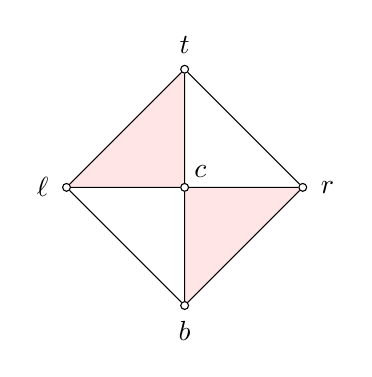
\begin{tikzpicture}[scale=1.5]

      \coordinate (t) at (0,1);
      \coordinate (l) at (-1, 0);
      \coordinate (r) at (1,0);
      \coordinate (b) at (0,-1);
      \coordinate (c) at (0,0);
      \fill[red!20!white, opacity=.5] (t) -- (l) -- (c) -- (t) (r)
      -- (c) -- (b) -- (r);

      \begin{scope}[every node/.style={draw, circle, inner sep=1pt,
          fill=white}]
        \node (t) at (t) {};
        \node (r) at (r) {};
        \node (l) at (l) {};
        \node (b) at (b) {};
        \node (c) at (c) {};
      \end{scope}


      \node[above, yshift=2pt] () at (t) {$t$};
      \node[right, xshift=3pt] () at (r) {$r$};
      \node[left, xshift=-3pt] () at (l) {$\ell$};
      \node[below, yshift=-2pt] () at (b) {$b$};
      \node[above right] () at (c) {$c$};

      \draw (t) -- (l) -- (b) -- (r) -- (t) (t) -- (c) -- (b) (l) --
      (c) -- (r);
    \end{tikzpicture}
  \end{figure}
  The simplices are as follows (Note, we'll use $\ip{v_1, v_2,
    \ldots, v_n}$ to denote ``the convex hull of $\set{v_1, v_2,
    \ldots, v_n}$'').
  \begin{enumerate}
    \item The 0-simplices: $K^0 = \set{\ip{t}, \ip{\ell}, \ip{b},
      \ip{r}, \ip{c}}$
    \item The 1-simplices: $K^1 = \set{\ip{t,\ell}, \ip{\ell, b},
      \ip{b, r},
      \ip{r, t}, \ip{t,c}, \ip{\ell, c}, \ip{b,c}, \ip{r,c}}$
    \item The 2-simplices: $K^2 = \set{\ip{t,\ell,c},
      \ip{b,r,c}}$.
  \end{enumerate}
  One can verify the axioms are satisfied. The underlying space is
  just all of the stuff except for the interior of the two white
  simplices, $\ip{t,r,c}$ and $\ip{b,\ell, c}$.
\end{example}
Now another definition.
\begin{definition}[Locally finite]
  Let $K$ be a simplicial complex. Then we say $K$ is
  \emph{locally finite} if for all 0-simplices $\sigma \in K$,
  $\sigma$ is a vertex of only finitely-many simplices of $K$.
\end{definition}
If one is not careful, this definition for locally-finite can create
some unexpected collections being referred to as ``simplicial
complexes.'' Of course, the weak topology is meant to prevent
silly situations such as these, but we'll pretend it doesn't exist for
the time being. This allows us to construct some PL-flavored
structures that seem germane to examining wild knots in a way that's
agnostic to the pathology at the wild point.
\begin{example}\label{ex:locally-finite-problem}
  Consider a proposed simplicial complex defined as follows.
  \begin{leftbar}
    \begin{enumerate}
      \item For all $n \in \NN$, let $I_n$ be defined by
        \[
        I_n = \bk{\frac{1}{2^n},\ \frac{1}{2^{n-1}}}
        \]
        Observe these are all $1$-simplices.
      \item Also define
        \[
        a_n = \set{\frac{1}{2^n}} \qquad\qquad\qquad\qquad b_n =
        \set{\frac{1}{2^{n-1}}}
        \]
        and
        \[
        I_\infty = \set{0}.
        \]
        Observe these are all $0$-simplices. Also note that $\partial
        I_n = a_n \cup b_n$.
    \end{enumerate}
    Let $S = I_\infty \cup \bigcup_{n \in \NN} \set{I_n, a_n, b_n}$
    (just scooping up all the items defined above). Is this a valid
    simplicial complex? Is it locally finite? \qedhere
  \end{leftbar}
\end{example}
\begin{sproof}[Sketch]
  We break the statement into parts. The results are straightforward,
  we have just sought to be exhaustive for completeness.
  \begin{leftbar}
    \textbf{Claim 1:} The collection $S$ defined in the question is a
    valid simplicial complex.

    \noindent \textbf{Proof of Claim 1:}
    \begin{enumerate}
      \item First, we verify that for all $\sigma \in K$, if $\tau$ is
        a face of $\sigma$, then $\tau \in K$.

        Let $\sigma \in K$ be arbitrary. We have two sub-cases.
        \begin{enumerate}[label=\arabic*)]
          \item Suppose $\sigma$ is a 0-simplex. Then $\sigma$ is its
            only face, so the claim holds.
          \item Suppose $\sigma$ is a 1-simplex. Then by construction,
            there exists $n \in \NN$ such that $\sigma =
            \bk{\frac{1}{2^n}, \frac{1}{2^{n-1}}}$. Hence the faces of
            $\sigma$ are $a_n = \set{\frac{1}{2^n}}$ and $b_n =
            \set{\frac{1}{2^{n-1}}}$, both of which are elements of $S$
            (by construction).
        \end{enumerate}
        Hence we see that the first condition is satisfied.
      \item Let $\sigma_1, \sigma_2 \in K$ be arbitrarily chosen. We
        want to show that if $\tau = \sigma_1 \cap \sigma_2 \neq
        \varnothing$, then $\tau$ is a face of both $\sigma_1$ and
        $\sigma_2$.

        First, note that if $\sigma_1 = \sigma_2$, then the claim is
        trivial. Hence suppose $\sigma_1 \neq \sigma_2$. We proceed by
        casework.
        \begin{enumerate}[label=\arabic*)]
          \item Suppose $\sigma_1$, $\sigma_2$ are both 0-simplices.
            Then since $\sigma_1 \neq \sigma_2$, we have $\sigma_1
            \cap \sigma_2 = \varnothing$, so the claim is satisfied
            vacuously.
          \item Now suppose one of $\sigma_1, \sigma_2$ is $I_\infty$.
            Note that for any $n \geq 0$, $I_\infty$ is disjoint from
            \emph{each} of $a_n$, $b_n$, and $I_n$. Hence $\sigma_1 \cap
            \sigma_2 = \varnothing$, so in this case the claim is also
            satisfied vacuously.
          \item Now suppose at least one of $\sigma_1, \sigma_2$ is not
            a 0-simplex, and that neither $\sigma_1, \sigma_2$ is
            $I_\infty$.\footnote{This is wordy, but we're just taking
            the complement of the two cases we've already done.} One can
            verify the following:
            \begin{enumerate}[label=\roman*)]
              \item Suppose one of $\sigma_1$, $\sigma_2$ is a 0-simplex
                and the other is a 1-simplex. Without loss of
                generality, let $\sigma_1$ be the 1-simplex and
                $\sigma_2$ be the 0-simplex. Then $\sigma_1$ is of the
                form $I_n = \bk{\frac{1}{2^n},\ \frac{1}{2^{n-1}}} =
                \ip{a_n \cup b_n}$ for some $n$ (recall, $a_n$, $b_n$
                were defined as 1-element sets). Then $\sigma_1 \cap
                \sigma_2 \neq\varnothing$ iff $\sigma_2$ is one of
                $a_n$ or $b_n$, at which point the claim follows by
                construction of $S$.
              \item Suppose $\sigma_1$, $\sigma_2$ are of the form $I_n$,
                $I_m$ respectively, and without loss of generality,
                suppose $n > m$. Then observe we have $I_n \cap I_m
                \neq \varnothing$ iff $n = m+1$. In this case, we see
                $I_n \cap I_m = \set{\frac{1}{2^{n-1}}} =
                \set{\frac{1}{2^m}}$, which is an element of $S$ by
                construction.
            \end{enumerate}
        \end{enumerate}
        In any case, we see the condition is satisfied.
    \end{enumerate}
    It follows that $S$ is a valid simplicial complex.
  \end{leftbar}

  \begin{leftbar}
    \textbf{Claim 2:} $S$ is locally finite.

    \noindent \textbf{Proof of Claim:} By a similar argument to the
    above, one can verify that
    \begin{enumerate}
      \item For all $n \in \NN$, we have $I_\infty \cap a_n = I_\infty
        \cap b_n = I_\infty \cap I_n$. Hence $I_\infty$ is a vertex of
        exactly one simplex, namely itself.
      \item For all $n \in \NN$, $a_n$ is a vertex of $I_n$ and
        $I_{n+1}$. Similarly, for $n > 2$, $b_n$ is a vertex of
        $I_{n-1}$, $I_n$. For $n = 1$, $b_1$ is a vertex of $I_1$ and
        that's it.
    \end{enumerate}
    In any case, we see that the simplicial complex is locally finite.
  \end{leftbar}

  \begin{leftbar}
    \textbf{Claim 3:} $\abs{S} = [0,1]$.

    \noindent \textbf{Proof of Claim 3:} Let $x \in [0,1]$ be
    arbitrary. We want to show $\exists \sigma \in K$ such that $x \in
    \sigma$. We proceed by casework.
    \begin{enumerate}
      \item Suppose $x = 0$. Then $x \in I_\infty$, as desired.
      \item Suppose that $x \neq 0$. Then there exists $n \in \NN$ such
        that
        \[
        \frac{1}{2^{n}} \leq x \leq \frac{1}{2^{n-1}},
        \]
        from which we have $x \in I_n$.\footnote{
        To be extremely explicit: one can take $\log_2$ of each term in
        the inequality above; since $\log_2$ is monotonic, the
        ordering is preserved. Then, one can use the Archimedean
        property of the reals to obtain the existence of the desired
        $n$.}
    \end{enumerate}
    In either case, it follows that there exists $\sigma \in K$ such
    that $x \in \sigma$. Hence $[0,1] \subseteq \bigcup_{\sigma \in K}
    \sigma$. Now observe that by construction, for all $\sigma \in K$,
    $\sigma \subseteq [0,1]$. Hence $\bigcup_{\sigma \in K} \sigma =
    [0,1]$.

    Hence we have $\abs{S} = [0,1]$, as desired.
  \end{leftbar}
  In any case, we see that according to all of our definitions, this
  is a honest-to-goodness locally-finite simplicial complex.
\end{sproof}
As we mentioned way back in \cref{chap:intro}, one can construct
similar simplicial complexes in $\RR^n$. For instance, consider the
following collection in $\RR^2$:
\begin{figure}[H]
  \centering
  \includegraphics[scale=.5]{figures/wild/simp-comp-down.pdf}
  \caption{A ``locally-finite'' simplicial complex.}
\end{figure}
Analogous objects in $\RR^3$ seem like they could be very apt for
describing ``discrete'' wild knots, especially in light of
\cref{thm:discrete-diagram-countably-polygonal}. Of course, we must be
careful not to go \emph{too} far in this direction; for instance, we
would not want to include objects like the following:
\begin{example}[Non-example]
  Let $K = \set{\sigma_i}$ be a collection of linear simplices defined
  by
  \[
    K = \set{\set{x} \MID x \in \RR}. \qedhere
  \]
\end{example}
This particular behavior could be constrained by requiring that $K$ be
countable, but that would still allow for complexes like the
following:
\begin{example}[Non-example]
  Let $K = \set{\sigma_i}$ be a collection of linear simplices defined
  by
  \[
    K = \set{\set{x} \MID x \in \QQ}. \qedhere
  \]
\end{example}
Inspired by these examples (but also by wanting to prevent the
non-examples given above), we imagine we could achieve the desired
effects by looking at something like the following (note, we encourage
the reader to improve upon our naming conventions):
\begin{definition}[A proposed definition]
  Let $K = \set{\sigma_i}$ be a simplicial complex. Define $K$ to be
  \emph{almost locally finite} if it is locally finite at all but
  finitely-many $0$-simplices.
\end{definition}
Or maybe something like the following:
\begin{definition}[Another proposed definition]
  Let $K = \set{\sigma_i}$ be a locally-finite simplicial complex.
  Define a \emph{feral point} of $K$ to be a $0$-simplex $\triangle^0
  \in K$ such that for all $\varepsilon > 0$, there exists
  infinitely-many $\sigma_i \in K$ such that
  $B_\varepsilon(\triangle^0) \cap \sigma_i \neq \varnothing$. Then
  endow $K$ with the subspace topology, and call $K$
  \emph{countably-PL} if there are only finitely-many feral points.
\end{definition}
We'd be interested in seeing if any of these proposed definitions
provide us \emph{objects} for a new category. Morphisms would be
similar to PL maps, only now with extra requirements to respect the
``feral'' structure, e.g.\ feral points map to feral points, plus
maybe some analogue to the star condition at these points.

We hope that future work in this direction might help to shed light on
deeper structure to knots. We are particularly excited about the
implications of \cref{chap:connections-to-sn}, and wonder whether they
can be generalized to \emph{everywhere-wild} knots. In particular, to
study these ``discrete'' knots we used symmetry groups of discrete
sets. We wonder whether continuous symmetry groups could be used to
study wild knots, which (in some sense) have ``continuous''
collections of crossings (although it seems we lose transverseness).

We'd also be interested in seeing deeper study of feral points,
particularly diagrammatic invariants for distinguishing them from wild
points. Lastly, we'd like to see a careful proof of an analogue to
Reidemeister's theorem in this new context, as well the development of
a new, slightly-stronger category in which to study our embeddings.



% naturally suited to studying well-behaved wild knots


% To the best of our knowledge, not many
% --- the question hasn't really been broached before. Our goal for this
% section is to very briefly remind the reader of some of the properties
% of our three categories, and point out ways in which PL could be
% extended to include some moderately well-behaved wild knots.

% {\color{blue} Just some short blurb here will suffice!}

%%% Local Variables:
%%% TeX-master: "../../kobayashi-thesis"
%%% End:



% Appendix

\part{Appendix}\label{part:appendix}

\appendix

\chapter{A Gallery of Some 3D Representations of Feral
  Knots}\label{chap:feral-gallery}
\def\figdir{figures/feral-gallery}
\def\otherfigdir{figures/unknotting-moves-and-combinatorial-representations}
The following theorem is proven in \cite{Crowell1963} (Appendix I,
pg.\ 147).
\begin{theorem}\label{thm:c1-suffices}
  Let $K$ be a knot in $\RR^3$ which is rectifiable and which is given
  as the image of a periodic vector-valued function $p(s) = (x(s),
  y(s), z(s))$ of arc length $s$ whose derivative $p'(s) = (x'(s),
  y'(s), z'(s))$ exists and is continuous for all $s$. Then $K$ is
  tame.
\end{theorem}
From what we can tell, the rectifiability condition is actually
superfluous, as it follows directly from the $C^1$ hypothesis. $C^1$
implies bounded variation, which in turn implies rectifiability. We
imagine \cite{Crowell1963} were simply trying to keep the prerequisite
knowledge to a minimum. In any case, we restate the result as follows.
\begin{theorem}
  Let $K : S^1\into \RR^3$. Then if $K$ is $C^1$, $K$ is tame.
\end{theorem}
We'll cite this freely in the below.


\section{Countable Twists}
\begin{example}[Countable Twists]~
  \begin{itemize}
    \item Description: A countable \# of twists
    \item Example countable polygonal representation
      \begin{figure}[H]
        \centering
        \includegraphics[angle=-90]{\otherfigdir/countable-r1-v2.pdf}
        \caption{Countable Polygonal Representation}
      \end{figure}
    \item Proof of tameness, method 1: Use Reidemeister I moves and
      \cref{thm:uniformly-convergent-ambient-isotopy}
    \item Proof of tameness, method 2: Explicit, $C^1$ 3D parameterization
      as an arc: $f : [-\pi,\pi] \into \RR^3$, parameters $r, \omega$.
      \[
      f(\theta) =
      \begin{cases}
        \begin{bmatrix}
          r \theta^3 \cos\pn{\frac{\omega}{\theta}} \\
          r \theta^3 \sin\pn{\frac{\omega}{\theta}} \\
          \theta^2
        \end{bmatrix} & \theta \geq 0 \\
        -f(-\theta) & \theta < 0
      \end{cases}
      \]
      $C^1$: all of $(-\pi, \pi)$. Can be extended past $\pm \pi$
      easily.
      \begin{figure}[H]
        \centering
        \includegraphics[scale=.25]{\figdir/countable-3d-twists-side.pdf}
        \caption{Perspective view}
        \label{fig:twists-perspective}
      \end{figure}
      \begin{figure}[H]
        \centering
        \includegraphics[scale=.25]{\figdir/countable-3d-twists-top.pdf}
        \caption{Top view}
        \label{fig:twists-top}
      \end{figure}
    \item Proof of tameness, method 3: Employ the top-down view and
      apply \cref{prop:replacing-by-same-endpoints}.
  \end{itemize}
\end{example}

\section{Countable Reidemeister II}
\begin{example}[Countable Reidemeister II]~
  \begin{itemize}
    \item Description: A countable \# of Reidemeister II's
    \item Example countable polygonal representation
      \begin{figure}[H]
        \centering
        \includegraphics[angle=-90]{\otherfigdir/countable-r2-v2.pdf}
        \caption{Countable Polygonal Representation}
      \end{figure}
    \item Proof of tameness, method 1: Use Reidemeister II moves and
      \cref{thm:uniformly-convergent-ambient-isotopy}, or
      alternatively, using
      \cref{thm:countable-gluing-ambient-isotopies} in two steps.
    \item Proof of tameness, method 2: Explicit, $C^1$ 3D parameterization
      as an arc: $f : [-\pi,\pi] \into \RR^3$, parameters $r, \omega$.
      \[
      f(\theta) =
      \begin{cases}
        \begin{bmatrix}
          r \theta^3 \cos\pn{\frac{\omega}{\theta}} \\
          \theta^2
          \theta^2
        \end{bmatrix} & \theta \geq 0 \\
        \begin{bmatrix}
          -r \theta^3 \cos\pn{\frac{\omega}{\theta}} \\
          -\theta^2
          \theta^2
        \end{bmatrix} & \theta < 0
      \end{cases}
      \]
      $C^1$: everywhere on $(-\pi, \pi)$. Can be extended past $\pm
      \pi$ easily.
      \begin{figure}[H]
        \centering
        \includegraphics[scale=.25]{\figdir/countable-3d-r2-perspective.pdf}
        \caption{Perspective view}
        \label{fig:countable-r2-perspective}
      \end{figure}
      \begin{figure}[H]
        \centering
        \includegraphics[scale=.25]{\figdir/countable-3d-r2-side.pdf}
        \caption{Side view}
        \label{fig:countable-r2-side}
      \end{figure}
      \begin{figure}[H]
        \centering
        \includegraphics[scale=.25]{\figdir/countable-3d-r2-top.pdf}
        \caption{Top view}
      \end{figure}
    \item Proof of tameness, method 3: Employ the top-down view and
      apply \cref{prop:replacing-by-same-endpoints}.
  \end{itemize}
\end{example}







%%% Local Variables:
%%% TeX-master: "../../kobayashi-thesis"
%%% End:

\chapter{A Crash Course in PL Topology}\label{appendix:pl-topology}
\epigraph{What is the big-picture idea of Linear Algebra? Reduce
  infinite spaces to finite descriptions. That is it---\emph{this} is
  the meaning of a basis!}{---Weiqing Gu}
\def\figdir{figures/appendix/}

For our purposes today, we can think of Piecewise-Linear Topology as
``the business of trying to study continuous topological objects by
approximating them with linear (more accurately, affine) structures.''
Because such structures can be given finite descriptions, there is a
sense in which this will bring a more ``discrete'' flavor to our
topological objects. Of particular importance will be the concept of a
\emph{simplicial complex}, what it means for one to be \emph{locally
  finite}, and how we can use this to build up our understanding of
knots. We'll begin by discussing some vocabulary. % The exposition here
% follows that in \cite{Sakai2013} fairly closely; see there for more
% details.\footnote{For our personal tastes, we found \cite{Sakai2013} a
%   bit difficult to read, especially given the sparsity of diagrams /
%   visuals. However, we did find it to be quite thorough.}

\section{Affine Sets}
Really we'll only be interested in convex sets for today. But to
define them, we need the concept of \emph{affine independence}, so it
seemed reasonable to do a brief primer on \emph{affine} topics while
we're at it.

Everything in the below should be general over any Banach space with
field $\RR$, but for today, we'll only consider $\RR^n$.% Note, in the
% below, we'll actually often write $\RR^m$ since we'll use $n$ to refer
% to an $n$-cell.
\begin{definition}[Affine Set]
  Let $F \subseteq \RR^n$. Then $F$ is called a \emph{affine set}
  (also sometimes called a \emph{flat}, but we won't use that here) if
  for all $x,y \in F$ and $t \in \RR$, we have
  \[
    \bk{1-t} x + ty \in F.
  \]
  Geometrically, ``every line through two points in $F$ is itself a
  subset $F$.''
\end{definition}
Note, this is essentially just a linear subspace that we allow to be
shifted so as to not include the $0$ vector. For instance:
\begin{figure}[H]
  \centering
  \includegraphics{figures/wild/affine-set.pdf}
  \caption[An affine set]{An affine set. The black circle indicates a
    point of intersection.}
  \label{fig:affine-set}
\end{figure}
\noindent is an affine set. This is encoded in the following
proposition.
\begin{proposition}\label{prop:affine-to-linear}
  Let $F \subseteq \RR^n$ be an affine set. Then for arbitrary $x \in
  F$, $F - x = \set{v - x \MID v \in F}$ is a linear subspace of
  $\RR^n$.
\end{proposition}
As an example, imagine shifting the plane in \cref{fig:affine-set}
down to the origin.

Just as we have a notion linear independence for vector spaces, we
have affine independence for affine sets.
\begin{definition}[Affine Independence]
  Let $\set{v_i}_{i=1}^n \subseteq \RR^n$. Then we say $\set{v_i}$
  are \emph{affinely-independent} iff % for all $\set{t_i}_{i=1}^n \in
  % \RR$, if
  % \[
  %   \sum_{i =1}^n  t_i v_i = 0 \qquad\qquad\text{and}\qquad\qquad
  %   \sum_{i=1}^n t_i = 0,
  % \]
  % then for all $i = 1, \ldots, n$, we have $t_i = 0$. This is
  % equivalent to requiring that
  for any $j = 1, \ldots, n$, the set
  \[
    \mc B_j = \set{v_i - v_j \MID % i= 1, \ldots, n \text{ where }
      i \neq j}
  \]
  is linearly independent.
\end{definition}
Note again, by \cref{prop:affine-to-linear}, this is just saying we
have a shifted linear subspace. We now define an analog to the
\emph{span} of a linearly independent set.
\begin{definition}[Affine Hull]
  Let $A \subset \RR^n$ be arbitrary. Then the \emph{affine hull} of
  $A$, denoted $\aff(A)$, is given by
  \[
    \aff(A) = \set{\sum_{i=1}^k t_i x_i \MID k \in \NN^{> 0},\
      \text{each}\ t_i \in \RR,\ x_i \in A, \text{ and } \sum_{i=1}^k
      t_i = 1% \ \text{and each}\ t_i \in \RR \text{ and }
      % x_i \in A
    }. \qedhere
  \]
\end{definition}
Note, we require $k > 0$ so that we don't accidentally pick up the
$0$ vector. One can use \cref{prop:affine-to-linear} to verify the
following:
\begin{proposition}
  Let $X \subseteq \RR^n$, and let $v \in F$. Then $\aff(X) - v =
  \vspan{X-v}$.
\end{proposition}
This formalizes our intuition that the affine hull is essentially a
shifted version of linear span. Finally, we introduce the analog to
linear transformations, namely \emph{affine maps}. These are
essentially just linear transformations followed by shifts; we'll use
them later to define PL maps.
\begin{definition}[Affine Map]
  Let $n,m \in \NN$, and let $A \subseteq\RR^n$, $B \subseteq \RR^m$
  be affine sets.\footnote{We make no assumptions about the relative
    sizes of $n,m$.} Then $f : A \to B$ is said to be affine iff for
  all $x,y \in A$ and all $t \in \RR$, we have
  \[
    f\pn{[1-t]x + ty} = [1-t] f(x) + tf(y). \qedhere
  \]
\end{definition}
Note, it was important to require both $A$ and $B$ to be affine in
order to guarantee we don't escape the domain / codomain in the
equation above. Again, we can reduce this to more familiar terms with
the following proposition.\footnote{This basically says ``affine maps
  can be thought of as shifting the affine set to the origin, applying
  a linear transformation, and then shifting it somewhere else.''}
\begin{proposition}
  Let $A \subseteq \RR^n$, $B \subseteq \RR^m$ be affine sets, and let
  $f : A \to B$. Then $f$ is affine iff for all $v_0 \in A$, the
  function $ f_{v_0} : \np{F - x_0} \to \np{B - f(x_0)}$ defined by
  \[
    f^{v_0}(v) = f(v + v_0) - f(v_0)
  \]
  is linear.
\end{proposition}
In interpreting the above, it might be helpful to note that by
\cref{prop:affine-to-linear}, $F - x_0$, $B - f(x_0)$ are linear
subspaces of $\RR^n, \RR^m$ respectively. Also note that on the
right-hand-side, we need the $+v_0$ in the $f(v + v_0)$ to ensure that
we are feeding $f$ something that really is in its domain.

Alright! This gives us everything we need to discuss convex sets and
simplicial complexes.

\section{Convex Sets, Simplices, \& Cells}
Convex sets are (more or less) restricted versions of affine sets.
Recall, in defining affine sets, we were essentially requiring that
any point $p$ on a line passing through points $x,y$ of our space $A$
had to also be an element of $A$. For convex sets we'll do something
similar, only instead of a \emph{line} passing through $x,y$, we look
at \emph{line segments} with endpoints $x,y$. This is encoded in the
following definition.
\begin{definition}[Convex Sets]
  Let $X \subseteq \RR^n$. Then we say $X$ is \emph{convex} iff for
  all $x,y \in X$ and $t \in [0,1]$, we have
  \[
    [1-t]x + ty \in X. \qedhere
  \]
\end{definition}
Note, affine sets are trivially convex. Just as we defined the affine
hull to mimic span for affine sets, we'll define the convex hull to
mimic span for convex sets.
\begin{definition}[Convex Hull]
  Let $A \subseteq \RR^n$. Then the \emph{convex hull} of $A$ is given
  by \footnotesize
  \[
    \ip{A} = \set{\sum_{i=1}^k t_i x_i \MID t_1 + \cdots + t_k = 1,\
      \text{and}\ \np{\text{for all}\ i = 1, \ldots, k,\ t_i \geq 0\
        \text{and}\ x_i \in A}
    }. \qedhere
  \]
\end{definition}

\section{Simplices \& Cells and their Complexes}
Note, in this section, we mostly follow the exposition in J.\ L.\
Bryant's \emph{Piecewise Linear Topology}, which we found the most
readable of the sources we referenced.\footnote{Can be found here:
  \url{https://www.maths.ed.ac.uk/~v1ranick/papers/pltop.pdf}}

\begin{definition}[Simplex]
  Let $\set{v_i}_{i=1}^n$ be affinely independent in $\RR^m$. Then the
  convex hull $\sigma = \ip{\set{v_i}_{i=1}^n}$ is called an $n-1$
  \emph{simplex}.
\end{definition}
\begin{definition}[Face]
  Let $\sigma = \ip{v_i}_{i=1}^n$. Then for all subsets $J \subseteq
  \set{1, \ldots, n}$, we call $\tau = \ip{v_j}_{j\in J}$ a
  \emph{face} of $\sigma$. We will often denote this by $\tau
  <\sigma$.
\end{definition}
\begin{definition}[Convex Linear Cell]
  $A \subseteq \RR^m$ is called a \emph{convex linear cell} iff
  there exist $v_1, \ldots, v_k$ (\emph{not} necessarily affinely
  independent) such that
  \[
    A = \ip[]{\set{v_i}_{i=1}^k}.
  \]
  If $n$ is the size of a maximal affinely independent subset of
  $A$, we say $A$ is a \emph{convex linear $n-1$-cell}.
\end{definition}
\begin{remark}
  Note, every convex linear $n$-cell $A$ can be written as
  \[
    A = \bigcup_{i=1}^{\ell} \sigma_i
  \]
  where the $\sigma_i$ are $n$-simplices without any ``gaps''
  between them.
\end{remark}



\begin{definition}[Simplicial Complex]
  Let $K = \set{\sigma_i}$, where the $\sigma_i$ are all $k$-simplices
  in $\RR^n$. Then we call $K$ a \emph{simplicial complex} iff
  \begin{enumerate}[label=(\arabic*)]
    \item (\textbf{Closure under faces}): For all $\sigma \in K$, for
      all faces $\tau \subseteq \sigma$, we have $\tau \in K$ as well.
    \item (\textbf{Intersection only along faces}): For all $\sigma,
      \tau \in K$, if $\sigma \cap \tau \neq \varnothing$, then
      $\sigma \cap \tau$ is a face of both $\sigma$ and $\tau$.
      \qedhere
  \end{enumerate}
\end{definition}
As an example, the following is a simplicial complex defined by taking
the standard tetrahedron and including each of its faces:
\begin{figure}[H]
  \centering
  \includegraphics[scale=.5]{\figdir/simplicial-complex.pdf}
  \caption{Example simplicial complex}
\end{figure}
In particular, $K = \set{V_1, A_1, A_2, A_3, A_4, e_1, e_2, e_3, e_4,
  e_5, e_6, A, B, C, D, \set{}}$.

The following proposed ``complex'' fails condition (2):
\begin{figure}[H]
  \centering
  \includegraphics{\figdir/simplex-collision.pdf}
  \caption{An example of a collection $K$ that fails condition (2).}
\end{figure}
We can perform a resolution by subdividing faces until the condition
is regained:
\begin{figure}[H]
  \centering
  \includegraphics{\figdir/simplex-collision-resolution-1.pdf}
  \caption{Subdividing to resolve the problem.}
\end{figure}
\begin{figure}[H]
  \centering
  \includegraphics{\figdir/simplex-collision-resolution-2.pdf}
  \caption{The new complex.}
\end{figure}
\begin{definition}[Polyhedron]
  Let $K = \set{\sigma_i}$ be a simplicial complex. Then the
  \emph{polyhedron} of $K$ (also called the \emph{underlying space} of
  $K$), denoted $\abs{K}$, is defined by
  \[
    \abs{K} = \bigcup_{\sigma \in K} \sigma. \qedhere
  \]
\end{definition}
We think of $\abs{K}$ as being endowed with the \emph{weak} topology,
which (given some niceness constraints) coincides with the subspace
topology.
\begin{definition}[Weak topology]
  Let $K$ be a simplicial complex. Define the \emph{weak topology} on
  $\abs{K}$ as follows:
  \begin{leftbar}
    Let $U \subseteq \abs{K}$ be arbitrary. Then we say $U$ is open
    iff for all $\sigma_i\in K$, $U \cap \sigma_i$ is open in
    $\sigma_i$. \qedhere
  \end{leftbar}
\end{definition}
The appropriate niceness constraint is provided by \emph{local
  finiteness}. This is defined slightly differently in different
texts.
\begin{definition}[Locally Finiteness]\label{def:locally-finite}
  Let $K = \set{\sigma_i}$ be a simplicial complex. Then we say $K$ is
  \emph{locally finite} if for all $0$-simplices $v \in K$, there
  exists $\varepsilon > 0$ such that there exists only finitely-many
  $\sigma_i$ for which
  \[
    \sigma_i \cap B_\varepsilon(v) = \varnothing.
  \]
\end{definition}
Note, other sources might define local finiteness in a different
manner. Namely,
\begin{definition}[Local Finiteness (Alt.)]\label{def:locally-finite-bad}
  Let $K$ be a simplicial complex. Then we say $K$ is \emph{locally
    finite} if for all $0$-simplices $v \in K$, there exists only
  finitely-many $\sigma_i$ such that $v$ is a vertex of $\sigma_i$.
\end{definition}
As far as we can tell, these conditions are not equivalent, but we
could be missing something here. For instance, under
\cref{def:locally-finite-bad}, what's to stop us from something like
the following?
\begin{leftbar}
  \textbf{Non-example:} Let $K = \set{\sigma_i}$ be defined by
  \[
    K = \set{\set{x} \MID x \in [0,1]}.
  \]
\end{leftbar}
Naively, this appears to satisfy all of the axioms for a simplicial
complex. Closure under faces is trivially satisfied. And all of our
simplices are disjoint, so ``intersection only along faces'' is
satisfied as well. But under \cref{def:locally-finite}, this is
\emph{not} locally finite, while it is under
\cref{def:locally-finite-bad}.

Anyways, we have the following proposition, which we do not prove.
\begin{proposition}
  Let $K$ be a simplicial complex that is locally finite in the sense
  of \cref{def:locally-finite}. Then $A \subseteq \abs{K}$ is closed
  in $\ms T_{\rm weak}$ iff it is closed in $\abs{K}$ with the
  subspace topology on $\RR^n$ (where $n$ is the maximal dimension of
  a simplex in the complex).
\end{proposition}

\begin{definition}[Subcomplex]
  Let $K$ be a simplicial complex. Then $L \subseteq K$ is said to be
  a \emph{subcomplex} if it is a simplicial complex.
\end{definition}
\begin{definition}[Boundary subcomplex]
  Let $K$ be a simplicial complex. Then for all $\sigma \in K$, we
  define the \emph{boundary subcomplex} of $\sigma$ by
  \[
    \dot{\sigma} = \set{\tau \MID \tau \neq \sigma}. \qedhere
  \]
\end{definition}
\begin{definition}[Interior]
  The \emph{interior} of $\sigma$ is defined by
  \[
    \accentset{\circ}{\sigma} = \sigma - \abs{\dot{\sigma}}. \qedhere
  \]
\end{definition}

\begin{definition}[Subdivision]
  Let $K_1, K_2$ be simplicial complexes. Then we say $K_1$ is a
  \emph{subdivision} of $K_2$ iff
  \begin{enumerate}
    \item $\abs{K_1} = \abs{K_2}$, and
    \item For all $\sigma \in K_1$, we have $\sigma \in K_2$ as well.
  \end{enumerate}
  Often, subdivision is denoted by $\prec$.
\end{definition}

We now define sensible morphisms for our complexes.
\begin{definition}[Simplicial Map]
  Let $K, L$ be simplicial complexes, and let $f : \abs{K} \to
  \abs{L}$. Then we call $f$ a \emph{simplicial map} iff for all
  $\sigma \in K$, we have $f(\sigma) \in L$ (with the added condition
  that the vertices of $\sigma$ \emph{must} be mapped to the vertices
  of $f(\sigma)$).
\end{definition}
\begin{proposition}
  A simplicial map is fully determined by where it sends each of the
  vertices (0-simplices) of $K$.
\end{proposition}
\begin{definition}[Piecewise Linear]
  Let $K, L$ be simplicial complexes. Then a function $f : \abs{K} \to
  \abs{L}$ is said to be \emph{piecewise-linear} (or \emph{PL}) iff
  there exist subdivisions $K' \prec K$, $L' \prec L$ such that $f :
  K' \to L'$ is simplicial.
\end{definition}
\begin{definition}[PL Homeomorphism]
  Let $K, L$ be simplicial complexes. Then we say $f : \abs{K} \to
  \abs{L}$ is a \emph{PL homeomorphism} iff there exist subdivisions
  $K' \prec K$, $L' \prec L$ such that $f$ bijective \emph{and}
  simplicial.
\end{definition}
% Hopefully, this gives the reader enough background to navigate the
% rest
We collect some propositions.
\begin{proposition}\label{prop:compact-finite}
  Let $K$ be a simplicial complex, and let $A \subseteq \abs{K}$ be
  compact. Then there exists a finite subcomplex $L < K$ such that
  $A\subseteq \abs{L}$.
\end{proposition}
\begin{sproof}
  See
  Hatcher\footnote{\url{http://pi.math.cornell.edu/~hatcher/AT/ATapp.pdf}},
  Appendix A, Proposition A.1.
\end{sproof}
This gives us that knots are polygonal.
\begin{corollary}
  Let $K : S^1 \into \RR^3$ be a PL embedding. Then $K$ is polygonal.
\end{corollary}
\begin{sproof}[Sketch]
  Note, $K$ is continuous and $S^1$ is compact, hence $\fim{K}{S^1}$
  is compact. By \cref{prop:compact-finite}, it follows that
  $\fim{K}{S^1}$ consists of a finite union of polygonal segments.
\end{sproof}
Hopefully this has given the reader a bit of a sense for the basics of
PL topology. For more, we encourage referencing the works listed in
\cref{subsec:further-reading}.

 % In particular, the example we
% introduce in \cref{ex:locally-finite-problem} (reproduced in brief
% below) seems to be locally finite under \cref{def:locally-finite-bad},
% but \emph{not} under \cref{def:locally-finite}.
% \begin{example}
%   Consider a simplicial complex defined as follows. For all $n \in
%   \NN$, let
%   \[
%     I_n = \bk{\frac{1}{n+1},\ \frac{1}{n}}.
%   \]
%   Observe that
% \end{example}





% \begin{figure}[H]
%   \centering
%   \includegraphics{\figdir/simplex-collision-resolution-2.pdf}
%   \caption{Full resolution}
% \end{figure}


% To define radial interior and radial boundary, we first define them
% for convex linear $1$-cells and then generalize.
% \begin{definition}[Radial Interior and Radial Boundary of a $1$-Cell]
%   Let $x,y \in \RR^m$ with $x \neq y$. Then the \emph{radial
%     boundary} of $C = \ip{\set{x,y}}$, denoted $\partial C$, is
%   \[
%     \partial C = \set{x,y}.
%   \]
%   We define the \emph{radial interior} of $C$ (denoted $\rint C$;
%   this is the convention given in \emph{Sakai}) to be
%   \begin{align*}
%     \rint C
%     &= C \setminus \partial C \\
%     &= \ip{\set{x,y}} \setminus \set{x,y}. \qedhere
%   \end{align*}
% \end{definition}

% \begin{definition}[Radial Interior and Radial Boundary in
%   general]\label{def:rad-int-bdy}
%   Let $C$ be a convex linear $n$-cell. Then define
%   \[
%     \rint C = \set{x \in C\MID \forall y \in C,\ \exists z \in C \st
%       x \in \rint \ip{\set{y,z}}}.
%   \]
%   Then, we have
%   \[
%     \partial C = C \setminus \rint.
%   \]
%   Note, the definition of $\rint$ is equivalent to
%   \[
%     \rint C = \set{x \in C\MID \forall y \in C,\ \exists s > 0 \st
%       [1 + s] x -  sy \in C}.\qedhere
%   \]
% \end{definition}
% % An interlude for a few important propositions:
% % \begin{leftbar}
% \begin{proposition}
%   Let $C$ be a convex linear $n$-cell. Let $\cong$ denote
%   homeomorphism. Then we have
%   \[
%     \pn{C, \partial C} \cong (B^n, S^{n-1}).
%   \]
% \end{proposition}
% \begin{sproof}
%   See \emph{Sakai}, Corollary 3.5.6 and the commentary on page
%   134.
% \end{sproof}
% \begin{proposition}
%   For any simplex $C$, $C$ has the unique topology such that $f : C
%   \times C \times I \to C$ given by
%   \[
%     f(x,y,t) = [1-t]x + ty
%   \]
%   is continuous.
% \end{proposition}
% \begin{sproof}
%   See \emph{Sakai}, Corollary 3.5.8 and the commentary on page
%   134.
% \end{sproof}
% % \end{leftbar}
% % A few more propositions before we continue.
% \begin{proposition}[Minimal Generating Set]\label{prop:min-gen-set}
%   Let $C \subset \RR^m$ be a convex linear $n$-cell. Then there
%   exists a minimal set $C^{(0)}$ such that
%   \begin{enumerate}
%     \item $\ip{C^{(0)}}  = C$, and
%     \item If $n > 0$ (i.e., $C$ is not a $0$-cell), then $C^{(0)}
%       \subset \partial C$.
%   \end{enumerate}
% \end{proposition}
% \begin{proof}
%   See \emph{Sakai}, Proposition 4.1.2 (page 136).
% \end{proof}
% \begin{definition}[Face at $x$]
%   Let $C$ be a convex linear $n$-cell, and let $x \in C$. Then the
%   \emph{face} of $C$ at $x$, denoted $C_x$, is defined by
%   \[
%     C_x = \set{y \in C \MID \exists s > 0 \st [1 + s]x - sy \in C.}
%     \qedhere
%   \]
% \end{definition}
% \begin{remark}
%   Note the similarity to \cref{def:rad-int-bdy} (Radial Interior and
%   Boundary). In particular, if $x \in \rint(C)$, then $C_x = C$.
% \end{remark}
% \begin{definition}[Face of a Cell]
%   Let $C \subset \RR^m$ be an $n$-cell, and let $D \subset \RR^m$ be
%   a $k$-cell with $k \leq n$. Then we say $D$ is a \emph{face} of
%   $C$ (denoted $D \leq C$) iff $\exists x \in C \st D = C_x$.
% \end{definition}
% % {\color{red} Are these needed?
% %   \begin{proposition}
% %     Let $C \subseteq \RR^m$ be a convex linear $n$-cell. Then $C_x$
% %     is a cell with $C_x^{(0)} = C^{(0)} = C^{(0)} \cap C_x$.
% %   \end{proposition}
% %   \begin{proposition}
% %     Maybe add proposition 4.1.6 here?
% %   \end{proposition}
% %   \begin{proposition}
% %     Let $A \subset \RR^m$ such that $A \neq \varnothing$ be
% %     arbitrary. Then $A$ is an $n$-cell iff all of the following are
% %     true:
% %     \begin{enumerate}
% %       \item $\dim \aff(C) < \infty$,
% %       \item For all $x,y \in C$ with $x \neq y$, $x + \RR_+(y - x)
% %         \not \subset C$, and {\color{red} what does this mean????}
% %       \item There exist finitely many non-constant affine
% %         functionals $f_1, \ldots, f_k : \aff(C) \to \RR$ such that
% %         \[
% %         C = \bigcap_{i=1}^k f^{-1}_i\pn{\RR_+}
% %         \]
% %     \end{enumerate}
% %   \end{proposition}
% % }

% \section{Simplicial Complexes}
% OK: from now on, we'll basically just be interested in simplicial
% complexes and their properties. The hope is that we'll be able to
% figure out which parts of Reidemeister's theorem can generalize nicely
% to wild knots.
% \begin{definition}[Cell Complex]
%   Let $I$ be an arbitrary indexing set, and let $K = \set{C_i}_{i\in
%     I}$ where each $C_i\subseteq \RR^m$ is a convex linear
%   $n_i$-cell (where $0 \leq n_i \leq m$). Then we call $K$ a
%   \emph{convex linear cell complex} iff
%   \begin{enumerate}
%     \item (\textbf{Closure under subcell}): For all $C_i \in K$, we
%       have that for all subcells $D \leq C_i$, $D \in K$ as well.
%     \item (\textbf{Closure under intersection}): For all $C_i, C_j
%       \in K$ with $C_i \cap C_j \neq \varnothing$, we have
%       \[
%       C_i \cap C_j \leq C_i \qquad\qquad\text{and}\qquad\qquad
%       C_i \cap C_j \leq C_j. \qedhere
%       \]
%   \end{enumerate}
% \end{definition}
% \begin{definition}[Simplicial Complex]
%   Let $K$ be a convex linear cell complex. We call $K$ a
%   \emph{simplicial complex} iff all of the $C_i$ are simplices.
% \end{definition}
% \begin{definition}[Polyhedron of $K$]
%   We define the \emph{polyhedron} of $K$ (denoted $\abs{K}$) by
%   \[
%     \abs{K} = \bigcup_{C \in K} \rint C \qedhere
%   \]
% \end{definition}
% \begin{definition}[Whitehead Topology]
%   Let $U \subseteq \abs{K}$. Then we say $U$ is open iff for all $C
%   \in K$, $U \cap C$ is open in $C$.
%   % \[
%   %   \ms T_{\rm whit}= \set{}
%   % \]
% \end{definition}
% \begin{proposition}
%   Let $(X, \ms T)$ be an arbitrary topological space. Then for any
%   continuous function $f : \abs{K} \to X$, $f$ is continuous iff
%   $\forall C_i \in K$, $f|C_i$ is continuous.
% \end{proposition}
% \begin{definition}[Star of a simplex]
%   Let $K$ be a simplicial complex, and let $C_i \in K$ be fixed.
%   Then we define the \emph{star} of $C$ in $K$ by
%   \[
%     \mrm{St}(C_i, K) = \set{D \MID \exists D' \in K \st C_i \leq D'
%       \text{ and } D \leq D'}. \qedhere
%   \]
% \end{definition}
% \begin{remark}
%   It's very important that we have $D \leq D'$ and not $D'\leq D$.
%   We are looking at the set of all simplices $D$ such that
%   \emph{both} $C_i$ and $D$ are faces of some larger simplex $D'$.
%   % Note, sub-faces of $D$ aaaaaaaaaAAAAAAAAAAAAAAAAAAa {\color{red}
%   %   aaaaaaaaaaaaaaaaaa}
% \end{remark}



\section{Some Examples of Rigorously-Constructing Ambient
  Isotopies}\label{sec:rigorous-ambient-isotopy}
\def\figdir{figures/infinite-gauss-sequence/}

Rigorously constructing ambient isotopies can be tedious and
unpleasant. However, given that our focus is on trying to provide
rigorous foundations for working with \emph{topological} ambient
isotopies, we'll include some notes on this process below. As with the
rest of the material in the appendix, this is strictly optional.

\begin{proposition}\label{prop:pt-to-barycenter}
  Let $\triangle_0$ be an $n$-simplex, and let $x_0 \in
  \triangle_0^\circ$ be arbitrary. Denote the barycenter of
  $\triangle_0$ by $c_0$. Then there exists an ambient isotopy
  $\ms{C}_{x_0} : [0,1] \times \RR^n \to \RR^n$ such that
  $\ms{C}_{x_0}$ is identity outside of $\triangle_0^\circ$ and
  $\ms{C}_{x_0}(1, x_0) = c_0$.
\end{proposition}
\begin{proof}
  Let $p \in \triangle_0^\circ$ be arbitrary. Then there exists a
  unique ``anchor point'' $a_p \in \partial \triangle_0$ such that
  there exists $s_p \in [0,1]$ such that $p = s_p \cdot x_0 +
  (1-s_p) \cdot a_p$. Note, this is equivalent to saying that
  $a_p, p, x_0$ are \emph{colinear} and either $p = a_p$, $p =
  x_0$, or $p$ is \emph{strictly} between $a_p$ and $x_0$. These
  lines are drawn in \emph{light orange} in
  \cref{fig:pt-to-barycenter}.


  \textbf{Claim:} Let $x(t) = t \cdot c_0 + (1-t)x_0$ (note, this
  is the straight-line homotopy from $x_0$ to $c_0$). Then the
  desired ambient isotopy $\ms C_{x_0}$ is given by
  \[
    \ms{C}_{x_0}(t, p) = s_p \cdot x(t) + (1-s_p) \cdot a_p
    \tag{$\forall p \in \triangle_0$}.
  \]
  See \cref{fig:pt-to-barycenter} for an illustration.
  \begin{figure}[H]
    \centering
    \includegraphics[scale=1]{\figdir/pt-to-barycenter.pdf}
    \caption{The desired ambient isotopy}
    \label{fig:pt-to-barycenter}
  \end{figure}
  \textbf{Proof of Claim:} First, we show (a) that the proposed
  $\ms{C}_{x_0}$ doesn't send points outside of $\triangle_0$, (b)
  that we have identity on the boundary, and (c) that we indeed
  have an ambient isotopy.
  \begin{enumerate}
    \item We want to show $\ms{C}_{x_0}$ doesn't send points outside
      of $\triangle_0$. Note, $x(t) \in \triangle_0$ for all $t$. Also
      note that $s_p + (1 - s_p) = 1$ always. Since $a_p \in
      \triangle_0$ as well, this shows $\ms{C}_{x_0}$ is a convex
      combination of points in $\triangle_0$. Since $\triangle_0$ is
      convex, it follows that $\ms{C}_{x_0}(t,p) \in \triangle$ for
      all $t \in [0,1]$, $p \in \triangle_0$. \cmark

    \item We want to show $\ms{C}_{x_0}$ is identity on the boundary.
      Note that if $p \in \partial \triangle_0$, then $p = a_p$ and
      hence $s_p = 0$. It follows that $\ms{C}_{x_0}(t, \cdot)$ is
      identity on $\partial \triangle_0$. \cmark
    \item To show that $\ms{C}_{x_0}(t, x)$ is an ambient isotopy,
      we must demonstrate that it is identity at $t=0$, that the
      image of $\triangle_0$ at $t=1$ is the desired modified
      version, that $\ms{C}_{x_0}(t, \cdot)$ is a homeomorphism for
      each $t$, and finally, that $\ms{C}_{x_0}$ is continuous
      overall.
      \begin{enumerate}[label=(\roman*)]
        \item The desired properties at $t = 0, 1$ follow
          immediately from the definition.
        \item We want to show that $\ms{C}_{x_0}(t, \cdot)$ is a
          homeomorphism for each $t$. Hence, let $t_0 \in [0,1]$ be
          arbitrary. Write $x(t_0) = x_0 + \delta(t_0)$ (from the
          definition of $x(t)$ above, we have $\delta(t_0) = t_0(c_0 -
          x_0)$). Now, note that
          \begin{align*}
            \ms{C}_{x_0}(t_0, p)
            &= s_p \cdot (x_0 + t_0(c_0 - x_0)) + (1-s_p) a_p \\
            &= \pn[Big]{s_p x_0 + (1-s_p) a_p} + s_pt_0 (c_0 - x_0) \\
            &= p + s_p t_0(c_0 - x_0).
          \end{align*}
          Ok now the $\varepsilon$-$\delta$ part: Let $\varepsilon > 0$
          be given. Through some fairly unpleasant trig, one can find a
          $\delta_0 > 0$ such that $q \in B_{\delta_0}(p)$ implies the
          angle $\angle p x_0 q$ is arbitrarily small.
          Then  one can then show that the rays
          $\overrightarrow{x_0 p}$ and $\overrightarrow{x_0 q}$
          intersect $\partial \triangle_0$ at points that are
          arbitrarily close. From this, we can constraint $\abs{s_p -
          s_q} < \varepsilon$, and use this to show continuity.

          To see that $C_{x_0}(t_0, \cdot)$ has a continuous inverse,
          observe that $p$ and $\ms{C}_{x_0}(t_0, p)$ have the same
          anchor point $a_p$ and displacement parameter $s_p$. Thus,
          define
          \[
          \ms{C}^{-1}_{x_0}(t_0, p) = s_p x(t_0) - s_p t_0 (c_0 -
          x_0),
          \]
          and note that this is indeed a well-defined inverse, and the
          same continuity argument as above demonstrates that it is
          continuous.
        \item One can then directly verify that $\ms{C}_{x_0}$ is
          continuous. \qedhere
      \end{enumerate}
  \end{enumerate}
\end{proof}
The second lemma is similar. We omit some of the details of the
proof since they are similar to that given above.
\begin{proposition} \label{prop:barycenter-exchange}
  Let $\triangle_0, \triangle_1$ be $n$-simplices that share an $n-1$
  face, and let $c_0, c_1$ be the barycenters of $\triangle_0,
  \triangle_1$ respectively. Then there exists an ambient isotopy
  $\ms{S}_{0,1} : [0,1] \times \RR^n \to \RR^n$ such that
  $\ms{S}_{0,1}$ is fixed on $\RR^n - (\triangle_0 \cup
  \triangle_1)^\circ$, and $\ms{S}_{0,1}(1, c_0) = c_1$.
\end{proposition}
\begin{proof}\renewcommand{\qed}{\hfill$\square$}
  The same proof as above works when $\triangle_0, \triangle_1$
  are regular (see \cref{fig:barycenter-isotopy}). However, when
  $\triangle_0, \triangle_1$ are \emph{not} regular, we have some
  additional things to worry about. In particular, $\triangle_0
  \cup \triangle_1$ might not be convex, so we can't just do a
  ``straight-line'' ambient isotopy.
  \begin{figure}[H]
    \centering
    \includegraphics[scale=.8]{\figdir/barycenter-isotopy.pdf}
    \caption{The desired isotopy when the simplices are regular}
    \label{fig:barycenter-isotopy}
  \end{figure}

  If $\triangle_0 \cup \triangle_1$ is not convex, we must be a
  little more creative. In particular, we see that the ambient
  isotopy above (\cref{fig:barycenter-isotopy}) isn't actually the
  most natural choice. Instead, consider the following (see
  \cref{fig:barycenter-isotopy-nonconvex} for illustration):
  \begin{enumerate}[label=\arabic*)]\newcommand{\temd}{\text{---}\,}
    \item Let $\temd_{0,1} = \set{u_1 \cdots u_{n}}$ denote the
      shared $n-1$ face of $\triangle_0$ and $\triangle_1$. Let
      $v_0$ and $v_1$ be the vertices of $\triangle_0$ and
      $\triangle_1$ (respectively) such that $v_0, v_1 \not\in
      \temd_{0,1}$.
    \item Then note: for all $x_0 \in \triangle_0^\circ$, there
      exists a unique $y \in \temd_{0,1}$ such that $x_0$ is
      collinear with $v_0, y$. Similarly for $x_1 \in
      \triangle_1^\circ$.
    \item Now, for each $y \in \temd_{0,1}$, we join these lines
      with the following parameterization:
      \[
      Y(s) =
      \begin{cases}
        2s \cdot y\qquad\,\,\,\,\, + (1 - 2s)\cdot v_0 & s \in \bk{0, \frac{1}{2}}
        \\
        (2s - 1) \cdot v_1 + (2 - 2s)\cdot y & s \in \pb{\frac{1}{2}, 1}
      \end{cases}
      \]
      the two cases here are illustrated by the \emph{orange} and
      \emph{blue} lines in
      \cref{fig:barycenter-isotopy-nonconvex}. Note that
      $Y\pn{\frac{1}{2}} = y$. % {\color{red} How can I make the
      % notation here clearer? I feel I ought to index $Y$ by $y$.}
    \item Now we define our ambient isotopy $\ms{S}_{0,1}$. First,
      we need to look at the kinked line $Y_c(s)$ the barycenters
      of $\triangle_0, \triangle_1$ live on. The corresponding
      $s_0, s_1$ will be necessary in defining $\ms{S}_{0,1}$.


      Let's do it. Let $c_0, c_1$ be the barycenters of $\triangle_0,
      \triangle_1$ respectively. We want to show they really \emph{do}
      lie on the same $Y$. To that end, note that the line through
      $v_0, c_0$ to $\temd_{0,1}$ and the line from $v_1, c_1$ to
      $\temd_{0,1}$ both end at the barycenter of $\temd_{0,1}$ (to
      verify this, write everything in barycentric coordinates).
      Hence, the corresponding $Y$ (denote it $Y_c$) satisfies $c_0,
      c_1 \in Y_c([0,1])$. Thus there exists $s_0, s_1$ such that
      $Y_c(s_0) = c_0$, and $Y_c(s_1) = c_1$. In particular, one can
      show that $s_0 = \frac{1}{3}$, $s_1 = \frac{2}{3}$ independent
      of the choice of $\triangle_0, \triangle_1$.

      Now we can define $\ms{S}_{0,1}$ itself. To do so, we'll
      introduce a fairly complicated formula (which exposes more
      information about how we derived the formula) and then show
      that it simplifies from a complete mess to something very
      simple. Let $x \in (\triangle_0 \cup \triangle_1)^\circ$ be
      arbitrary. Write it as $Y(s_0)$ for some $Y$ as described
      above in step 3). We define $\ms{S}_{0,1}$ by
      \[
      \ms{S}_{0,1}(t, x) = \ms{S}_{0,1}(t, Y(s)) =
      \begin{cases}
        Y\pn{t\bk{s_1 - s_0 + s} + \bk{1-t}s} & s \in \bk{0,
          \frac{1}{2}} \\
        Y\pn{ \text{some mystery function!}
          % t\bk{\frac{1}{2} + ()}
        } & s \in \bk{\frac{1}{2}, 1},
      \end{cases}
      \]
      where we leave the reader to puzzle out what the mystery
      function is.
      % {\color{red} \Huge Return and finish}
  \end{enumerate}
  It follows that $\ms{S}_{0,1}$ is the desired ambient isotopy.
  \begin{figure}[H]
    \centering
    \includegraphics{\figdir/barycenter-isotopy-nonconvex-setup.pdf}
    \caption{An example where $\triangle_0 \cup \triangle_1$ is not
      convex (see \textbf{Important Note} below).}
    \label{fig:barycenter-isotopy-nonconvex}
  \end{figure}
  \textbf{Important Note:} Not all of the dotted lines are drawn in
  the final diagram, and I've removed the color-coding. I'm not
  terribly pleased with this, but it was getting to be too
  troublesome to do all of the trig arithmetic in TikZ to justify
  continuing onwards. The point is that one should imagine extending
  the reasoning of the first two diagrams, and observe that the
  barycenter gets where it needs to go.
\end{proof}

\begin{corollary}\label{cor:moving-through-simplices}
  Let $\triangle_0, \triangle_1, \ldots, \triangle_k$ be
  $n$-simplices such that for each $i = 0, \ldots, k-1$,
  $\triangle_{i}$ and $\triangle_{i+1}$ share an $n-1$-face. Let
  $x_0 \in \triangle_0$ and $x_1 \in \triangle_k$. Then there
  exists an ambient isotopy $H_{x_0, x_1} : [0,1] \times \RR^n \to
  \RR^n$ such that $H$ is fixed outside of $\bigcup_{i=0}^k
  \triangle_k^\circ$, i.e.
  \[
    H(t, x) = x \qquad\text{\rm whenever}\qquad x \in \RR^n -
    \bigcup_{i=0}^k \triangle_k^\circ,
  \]
  and $H(1, x_0) = x_1$.
\end{corollary}
\begin{proof}\renewcommand{\qed}{\hfill$\square$}
  Note, by \cref{prop:pt-to-barycenter}, there exists an ambient
  isotopy $\ms{C}_{x_0} : [0,1] \times \RR^n \to \RR^n$ that
  leaves $\RR^n - \triangle_0^\circ$ fixed, and takes $x_0$ to the
  barycenter $c_0$ of $\triangle_0$.

  Now, by \cref{prop:barycenter-exchange}, there exists a sequence
  of ambient isotopies $\ms{S}_{0,1}$, $\ms{S}_{1,2}$, $\ldots$,
  $\ms{S}_{k-1,k}$ taking the barycenter of $\triangle_0$ to that of
  $\triangle_1$, the barycenter of $\triangle_1$ to $\triangle_2$,
  and so on. For each $i \in \set{0, \ldots, k-2}$, let $f_i(x) =
  \ms S_{i,i+1}(1, x)$ It follows that $\ms S_{0,k}$ defined by
  \[
    \ms{S}_{0,k} =
    \begin{cases}
      \ms{S}_{0,1}\pn{k \cdot t, x} & t \in \bk{0, \frac{1}{k}} \\
      \ms{S}_{1,2}\pn{(k \cdot t) - 1, f_0(x)} & t \in
      \bk{\frac{1}{k}, \frac{2}{k}} \\
      \vdots & \\
      \ms{S}_{i,i+1}\pn{(k \cdot t) - i, \comp_{j=1}^{i-1} f_j(x)} &
      t \in \bk{\frac{i}{k}, \frac{i+1}{k}} \\
      \vdots & \\
      \ms{S}_{k-1,k}\pn{(k \cdot t) - (k-1), \comp_{j=1}^{k-2}
        f_j(x)} & t \in
      \bk{\frac{k-1}{k}, 1} \\
    \end{cases}
  \]
  can be shown to be a valid ambient isotopy.\footnote{Just apply
    the gluing lemma.}
\end{proof}
% \begin{figure}[H]
%   \centering
%   \includegraphics{\figdir/two-simplex-isotopy.pdf}
%   \caption{One way to deform the space to get $x_0 \to x_1$.}
% \end{figure}

  % \begin{lemma}
  %   Suppose $f : \RR^3 \to \RR^3$ is an orientation-preserving
  %   homeomorphism with $f(K) = P$. Then there exists an ambient
  %   isotopy $H : [0,1] \times \RR^n \to \RR^n$ such that $H(1, f)$
  %   fixes a 3-simplex.
  % \end{lemma}
  % \emph{Proof:} We construct the vertices of our simplex $[v_0 v_1
  % v_2 v_3]$. We have cases:
  % \begin{enumerate}[label=(\arabic*)]
  %   \item Suppose $f$ has a fixed point. Then let this be $v_0$.
  %   \item Else, we want to show there exists an ambient isotopy $H^0
  %     : [0,1] \times \RR^3 \to \RR^3$ such that $H^0(1, f(v_0)) =
  %     v_0$. We'll {\color{red} this part currently unfinished}
  %     % let $S \subseteq \RR^3$ be an arbitrary 3-simplex,
  %     % and let $v_0$ .
  %   \item Then consider the ambient isotopy $G : [0,1] \to \RR^3$
  %     that leaves $\RR^3 \setminus S$ fixed (only deforms the interior
  %     of $S$). {\color{red} Also unfinished}
  % \end{enumerate}

  % % \begin{lemma}
  % %   Let $\triangle_1, \triangle_2, \ldots, \triangle_n$ be a sequence of
  % %   $3$-simplices such that for each $k = 1,\ldots, n-1$, the
  % %   simplices $\triangle_{k}$ and $\triangle_{k+1}$ share a common
  % %   $2$-face. Now, let $x_0 \in \triangle_1$ and $x_1 \in \triangle_n$.
  % %   Then there exists an ambient isotopy $H : [0,1] \to \RR^3$ such
  % %   that $H$ is fixed outside the simplices, i.e.
  % %   \[
  % %     H(t, x) = x \qquad \text{\rm whenever } \qquad x \in \RR^3 -
  % %     \bigcup_{k=1}^n \triangle_k,
  % %   \]
  % %   and we have
  % %   \[
  % %     H(1, x_0) = x_1.
  % %   \]
  % % \end{lemma}
  % % \emph{Proof:}





% \begin{leftbar}
%   \begin{lemma}
%     Let all variables as quantified above, except choosing $K$
%     restricted to a connected subset of $S^1$ (think of this as
%     embedding an interval). \textbf{Further} suppose that $K$ is
%     wild at exactly one point $p$. Then the claim holds.
%   \end{lemma}
%   \emph{Proof of Lemma:} Let $\pn{V_k}_{k=0}^\infty$ be a nested
%   sequence of closed neighborhoods of $p$. Explicitly: each $V_k$ is
%   closed, and
%   \[
%     \bigcap_{k=0}^\infty V_k = \set{p} \qquad\qquad\qquad \text{and}
%     \qquad\qquad\qquad
%     \cdots \subseteq V_2 \subseteq V_1 \subseteq V_0.
%   \]
%   Since $K$ is ambient isotopic to a polygonal knot, there exists an
%   orientation-preserving homeomorphism $h : \RR^3 \to \RR^3$ such
%   that $h(K) = P$. Note, it follows that
%   \[
%     \bigcap_{k=0}^\infty h(V_k) = \set{h(p)} \qquad\qquad\qquad
%     \text{and} \qquad\qquad\cdots \subseteq h(V_2) \subseteq h(V_1)
%     \subseteq h(V_0).
%   \]
%   Since $P$ has only finitely many crossings, it follows that there
%   exists $N \in \NN$ such that for $n > N$, $P$ contains no
%   crossings in $h(V_n)$. Equivalently, $h(V_n) - P = h(V_n) - h(K) =
%   h(V_n - K)$ has trivial fundamental group.

%   {\color{red} this is unfinished}

%   \textbf{Claim:} There exists an ambient isotopy $f : \RR^3 \to
%   \RR^3$ such that $f(1, h(V_n)) = h(V_n)$ for all $n > N$.
% \end{leftbar}



%%% Local Variables:
%%% TeX-master: "../../kobayashi-thesis"
%%% End:

\chapter{Misc}\label{chap:misc}
\section{Solution to the Chessboard Problem}
\begin{sproof}[Solution]\label{sol:chessboard}
  \textbf{Claim:} No.\\

  \noindent \emph{Proof:} {Observe that there} are {25 black squares}
  and {24 white squares}. {Also} {note that every legal move takes} a
  {knight to} an {opposite-color square}. {Hence} {after moving all}
  the {knights}, {we}'{d have 25 on black} and {24 on white}, {which
    is} a {contradiction}. \hfill {$\jiong$}
  \renewcommand{\qed}{}
\end{sproof}
\section{\texttt{Julia} Code for the Countable Reidemeister I
  Example}\label{sec:Julia-for-countable-reidemeister-i}
\begin{lstlisting}
using Plots
using Colors
plotlyjs()

# r₁ is the big r for the circle this is based on.
#
# This function just computes the equation seen in our explicit
# parameterization of the countable reidemeister I knot. Note that
# this uses the form defined in terms of the matrix-vector equation,
# since we found it more tangible when prototyping.
function to_cartesian(θ; r₁=3)
    # This is the special "f(0)=0" case in our piecewise definition of
    # our function.
    if θ == 0
        return [r₁,0,0]
    end

    # Compute the radius of the smaller circle
    r₂ = abs(θ)^3
    x = r₁*cos(θ)
    y = r₁*sin(θ)

    # The radial vector is orthogonal to the tangent vector, hence
    # we can use it as one of the basis vectors for the orthogonal
    # frame.
    vperp = [x, y, 0]
    vperp /= sqrt((x^2 + y^2)) # Normalize it

    # Since the big circle lies in the xy-plane, the z direction is
    # also always one of the basis vectors for the orthogonal plane.
    zperp = [0,0,1]

    scale=2*π^2
    if θ > 0
        v_to_transform = [r₂*sin(scale/θ), r₂*cos(scale/θ), 0.0]
    else
        v_to_transform = [r₂*sin(-1*scale/θ), r₂*cos(scale/θ), 0.0]
    end

    # Rotate into the orthogonal plane
    R_mat = [zperp vperp [0.0; 0.0; 0.0]]
    v_out = (R_mat * v_to_transform) + [x,y,0]
    return v_out
end

step = .0001
θs = 0:step:π/2
θ₂s = reverse(-1 .* θs)


xyz_vals = to_cartesian.(θs)
xyz_opp = to_cartesian.(θ₂s) # The mirror image
append!(xyz_opp, xyz_vals)

xs = [p[1] for p in xyz_opp]
ys = [p[2] for p in xyz_opp]
zs = [p[3] for p in xyz_opp]

lcol= colorant"#D6D7D9"
bcol= colorant"#1D252C"

plot(camera=(60, 25), size=(1500,1000),
     legend=false, background_color=bcol,
     color = lcol)#, grid=false)#, axis=false, ticks=false)

plot!(xs, ys, zs, color=lcol, lw=.5)
\end{lstlisting}

\section{Combinatorial Representations}\label{app:combinatorial-representations}
\subsection{Cycle representations}
\begin{table}[H]
  \centering
  \small
  \begin{tabular}{clc}
    \toprule
    Index & Cycle representation & Order \\ \midrule
    $(3, 1)$ & $(-3, -2) (1, 2)$ & 2 \\
$(4, 1)$ & $(-3, -2i, 4, 3, i, -i, 2i)$ & 7 \\
$(5, 1)$ & $(-5, -4, -2, -3) (1, 2, 4, 3)$ & 4 \\
$(5, 2)$ & $(-5, -4, -2, -3) (1, 2, 4)$ & 12 \\
$(6, 1)$ & $(-2, -3i, 6i, -4i, 1, 2, 4i) (-6i, 3i, -5i, 5i)$ & 28 \\
$(6, 2)$ & $(-6, -2i, 4i) (-5i, 5i, -4i, 3i) (-3i, 1, 2i)$ & 12 \\
$(6, 3)$ & $(-6, 4i, 6) (-5, 5, -3i) (-1, 1, -2i, -4i) (2i, 3i)$ & 12 \\
$(6, 4)$ & $(-6, -5) (-3, -2) (1, 2) (4, 5)$ & 2 \\
$(6, 5)$ & $(-3, -2) (-5i, -4i) (5i, 6i) (1, 2)$ & 2 \\
$(7, 1)$ & $(-7, -6, -4) (-5, -2, -3) (1, 2, 4) (3, 6, 5)$ & 3 \\
$(7, 2)$ & $(-7i, 2i) (-6i, 4i, -4i, 5i) (-5i, 7i, -3i, 3i, -2i, i, -i, 6i)$ & 8 \\
$(7, 3)$ & $(-7, -6, -4, -5, -2, -3) (1, 2, 4) (3, 6, 5)$ & 6 \\
$(7, 4)$ & $(-7, -6, -2, -3, -5, -4) (1, 2, 4) (3, 6, 7, 5)$ & 12 \\
$(7, 5)$ & $(-7i, 6i, -4i, 3i, -5i, 7i) (-6i, 5i) (-3i, i, -i, 2i) (-2i, 4i)$ & 12 \\
$(7, 6)$ & $(-3, -5i, i, -i, 2i) (-7i, 7i, -2i, 4, 3, 6i, -6i, 5i)$ & 40 \\
$(7, 7)$ & $(-6, -4) (-3, -2i, 4, 7, 6, 3, 5i, -5i, i, -i, 2i)$ & 22 \\
$(8, 1)$ & $(-4, -5i, 8i, -6i, 3, i, -i, 2i, -3, -2i, 4, 6i) (-8i, 5i, -7i, 7i)$ & 12 \\
$(8, 2)$ & $(-2, 3i, 5i, 2, -4i, -8i, -7i, -5i, -1, 1) (-6i, -3i) (4i, 7i) (6i, 8i)$ & 10 \\
$(8, 3)$ & $(-4, -7i, 7i, -8i, 5i) (-3, -5i, 3, 6i, -2) (-6i, 1, 2, 4, 8i)$ & 5 \\
$(8, 4)$ & $(-5, -8i, 8i, -7i, 6i, -4, -6i, 3, i, -i, 2, 4, 7i, -2, -3)$ & 15 \\
$(8, 5)$ & $(-8, -4, -7) (-5, -2i, 4, 8, 5, i, -i, 2i, -3) (3, 6, 7)$ & 9 \\
$(8, 6)$ & $(-2, 3i, 5i, 2, -4i, -8i, -5i, -1, 1) (-7i, -3i, -6i) (4i, 7i, 6i, 8i)$ & 36 \\
$(8, 7)$ & $(-8, -7, -5) (-6, -2i, i, -i, 2i, -3i, 5, 4, 7, 6, 3i, -4)$ & 12 \\
$(8, 8)$ & $(-8, 7, -1, 1, -2, 3, -6i, -3, 5i, 8) (-7, 2, -4i)$ & 30 \\
$(8, 9)$ & $(-8, -6, -4i, 8, 7, 5, 3i, -5, -2i, 4i, -7) (-3i, 6, i, -i, 2i)$ & 55 \\
$(8, 10)$ & $(-5, -7i, 7i, -6i, 8i, -8i, 5, 3, 1, 2, 4, 6i, -4, -2, -3)$ & 15 \\
$(8, 11)$ & $(-2, 3i, 5i, 2, -4i, -8i, -7i, -3i, -6i, -5i, -1, 1) (4i, 7i) (6i, 8i)$ & 12 \\
$(8, 12)$ & $(-3, -5i, 8i, -6i, 1, 2, 4, 3, 6i, -2) (-8i, 5i, -7i, 7i)$ & 20 \\
$(8, 13)$ & $(-7, 4, -3, 5, -i, -2i, -4, 7) (-6, 2i, 3) (-5, 8i, 6, -8i)$ & 24 \\
$(8, 14)$ & $(-2, -3i, 6i) (-8i, 3i, -5i, 8i) (-7i, 7i, -6i, 1, 2, 4i) (-4i, 5i)$ & 12 \\
$(8, 15)$ & $(-8i, -5i, -6i, -i, -2i, -4i, -7i) (2i, 3i, 5i, 8i, 4i, 6i)$ & 42 \\
$(8, 16)$ & $(-6, 8i, 6, -i, -2, 3) (-3, 5i, 4i, 2, -4i, -7i)$ & 6 \\
$(8, 17)$ & $(-6, -8i, 8i, -7i, 3, 6, i, -i, 2i, -3, -5, -4, -2i, 4, 7i)$ & 15 \\
$(8, 18)$ & $(-5, -4, -2i, 4, 7, 3i) (-8i, 5, 8i) (-6i, 1, 2i, -3i, 6i)$ & 30 \\
$(8, 19)$ & $(-8, -7, 6, -5, 4, -6) (-4, -2, -3, 5, 7, 3, 1, 2)$ & 24 \\
$(8, 20)$ & $(-4, 6i, 8i, 7i, -2i) (-3, -5i, -7i, -6i, 5i, 4) (2i, 3, 1)$ & 30 \\
$(8, 21)$ & $(-6, 8i, 6, 7i, -2i, -4i, 1, 2i, -3i) (-7i, 3i, 5i, 4i)$ & 36 \\

    \bottomrule
  \end{tabular}
  \caption[Cycle presentations]{$\ms N_{\rm g.int}$ cycle
    presentations for knots up to $8$ crossings}
  \label{tab:cycle-gint}
\end{table}

\begin{table}[H]
  \centering
  \small
  \begin{tabular}{clc}
    \toprule
    Index & Cycle representation & Order \\ \midrule
    $(3, 1)$ & $(3^+_u, 2^+_u)(1^+_o, 2^+_o)$ & 2 \\
$(4, 1)$ & $(3^+_u, 2^-_u, 4^+_o, 3^+_o, 1^-_o, 1^-_u, 2^-_o)$ & 7 \\
$(5, 1)$ & $(5^+_u, 4^+_u, 2^+_u, 3^+_u)(1^+_o, 2^+_o, 4^+_o, 3^+_o)$ & 4 \\
$(5, 2)$ & $(5^+_u, 4^+_u, 2^+_u, 3^+_u)(1^+_o, 2^+_o, 4^+_o)$ & 12 \\
$(6, 1)$ & $(2^+_u, 3^-_u, 6^-_o, 4^-_u, 1^+_o, 2^+_o, 4^-_o)(6^-_u, 3^-_o, 5^-_u, 5^-_o)$ & 28 \\
$(6, 2)$ & $(6^+_u, 2^-_u, 4^-_o)(5^-_u, 5^-_o, 4^-_u, 3^-_o)(3^-_u, 1^+_o, 2^-_o)$ & 12 \\
$(6, 3)$ & $(6^+_u, 4^-_o, 6^+_o)(5^+_u, 5^+_o, 3^-_u)(1^+_u, 1^+_o, 2^-_u, 4^-_u)(2^-_o, 3^-_o)$ & 12 \\
$(6, 4)$ & $(6^+_u, 5^+_u)(3^+_u, 2^+_u)(1^+_o, 2^+_o)(4^+_o, 5^+_o)$ & 2 \\
$(6, 5)$ & $(3^+_u, 2^+_u)(5^-_u, 4^-_u)(5^-_o, 6^-_o)(1^+_o, 2^+_o)$ & 2 \\
$(7, 1)$ & $(7^+_u, 6^+_u, 4^+_u)(5^+_u, 2^+_u, 3^+_u)(1^+_o, 2^+_o, 4^+_o)(3^+_o, 6^+_o, 5^+_o)$ & 3 \\
$(7, 2)$ & $(7^-_u, 2^-_o)(6^-_u, 4^-_o, 4^-_u, 5^-_o)(5^-_u, 7^-_o, 3^-_u, 3^-_o, 2^-_u, 1^-_o, 1^-_u, 6^-_o)$ & 8 \\
$(7, 3)$ & $(7^+_u, 6^+_u, 4^+_u, 5^+_u, 2^+_u, 3^+_u)(1^+_o, 2^+_o, 4^+_o)(3^+_o, 6^+_o, 5^+_o)$ & 6 \\
$(7, 4)$ & $(7^+_u, 6^+_u, 2^+_u, 3^+_u, 5^+_u, 4^+_u)(1^+_o, 2^+_o, 4^+_o)(3^+_o, 6^+_o, 7^+_o, 5^+_o)$ & 12 \\
$(7, 5)$ & $(7^-_u, 6^-_o, 4^-_u, 3^-_o, 5^-_u, 7^-_o)(6^-_u, 5^-_o)(3^-_u, 1^-_o, 1^-_u, 2^-_o)(2^-_u, 4^-_o)$ & 12 \\
$(7, 6)$ & $(3^+_u, 5^-_u, 1^-_o, 1^-_u, 2^-_o)(7^-_u, 7^-_o, 2^-_u, 4^+_o, 3^+_o, 6^-_o, 6^-_u, 5^-_o)$ & 40 \\
$(7, 7)$ & $(6^+_u, 4^+_u)(3^+_u, 2^-_u, 4^+_o, 7^+_o, 6^+_o, 3^+_o, 5^-_o, 5^-_u, 1^-_o, 1^-_u, 2^-_o)$ & 22 \\
$(8, 1)$ & $(4^+_u, 5^-_u, 8^-_o, 6^-_u, 3^+_o, 1^-_o, 1^-_u, 2^-_o, 3^+_u, 2^-_u, 4^+_o, 6^-_o)(8^-_u, 5^-_o, 7^-_u, 7^-_o)$ & 12 \\
$(8, 2)$ & $(2^+_u, 3^-_o, 5^-_o, 2^+_o, 4^-_u, 8^-_u, 7^-_u, 5^-_u, 1^+_u, 1^+_o)(6^-_u, 3^-_u)(4^-_o, 7^-_o)(6^-_o, 8^-_o)$ & 10 \\
$(8, 3)$ & $(4^+_u, 7^-_u, 7^-_o, 8^-_u, 5^-_o)(3^+_u, 5^-_u, 3^+_o, 6^-_o, 2^+_u)(6^-_u, 1^+_o, 2^+_o, 4^+_o, 8^-_o)$ & 5 \\
$(8, 4)$ & $(5^+_u, 8^-_u, 8^-_o, 7^-_u, 6^-_o, 4^+_u, 6^-_u, 3^+_o, 1^-_o, 1^-_u, 2^+_o, 4^+_o, 7^-_o, 2^+_u, 3^+_u)$ & 15 \\
$(8, 5)$ & $(8^+_u, 4^+_u, 7^+_u)(5^+_u, 2^-_u, 4^+_o, 8^+_o, 5^+_o, 1^-_o, 1^-_u, 2^-_o, 3^+_u)(3^+_o, 6^+_o, 7^+_o)$ & 9 \\
$(8, 6)$ & $(2^+_u, 3^-_o, 5^-_o, 2^+_o, 4^-_u, 8^-_u, 5^-_u, 1^+_u, 1^+_o)(7^-_u, 3^-_u, 6^-_u)(4^-_o, 7^-_o, 6^-_o, 8^-_o)$ & 36 \\
$(8, 7)$ & $(8^+_u, 7^+_u, 5^+_u)(6^+_u, 2^-_u, 1^-_o, 1^-_u, 2^-_o, 3^-_u, 5^+_o, 4^+_o, 7^+_o, 6^+_o, 3^-_o, 4^+_u)$ & 12 \\
$(8, 8)$ & $(8^+_u, 7^+_o, 1^+_u, 1^+_o, 2^+_u, 3^+_o, 6^-_u, 3^+_u, 5^-_o, 8^+_o)(7^+_u, 2^+_o, 4^-_u)$ & 30 \\
$(8, 9)$ & $(8^+_u, 6^+_u, 4^-_u, 8^+_o, 7^+_o, 5^+_o, 3^-_o, 5^+_u, 2^-_u, 4^-_o, 7^+_u)(3^-_u, 6^+_o, 1^-_o, 1^-_u, 2^-_o)$ & 55 \\
$(8, 10)$ & $(5^+_u, 7^-_u, 7^-_o, 6^-_u, 8^-_o, 8^-_u, 5^+_o, 3^+_o, 1^+_o, 2^+_o, 4^+_o, 6^-_o, 4^+_u, 2^+_u, 3^+_u)$ & 15 \\
$(8, 11)$ & $(2^+_u, 3^-_o, 5^-_o, 2^+_o, 4^-_u, 8^-_u, 7^-_u, 3^-_u, 6^-_u, 5^-_u, 1^+_u, 1^+_o)(4^-_o, 7^-_o)(6^-_o, 8^-_o)$ & 12 \\
$(8, 12)$ & $(3^+_u, 5^-_u, 8^-_o, 6^-_u, 1^+_o, 2^+_o, 4^+_o, 3^+_o, 6^-_o, 2^+_u)(8^-_u, 5^-_o, 7^-_u, 7^-_o)$ & 20 \\
$(8, 13)$ & $(7^+_u, 4^+_o, 3^+_u, 5^+_o, 1^-_u, 2^-_u, 4^+_u, 7^+_o)(6^+_u, 2^-_o, 3^+_o)(5^+_u, 8^-_o, 6^+_o, 8^-_u)$ & 24 \\
$(8, 14)$ & $(2^+_u, 3^-_u, 6^-_o)(8^-_u, 3^-_o, 5^-_u, 8^-_o)(7^-_u, 7^-_o, 6^-_u, 1^+_o, 2^+_o, 4^-_o)(4^-_u, 5^-_o)$ & 12 \\
$(8, 15)$ & $(8^-_u, 5^-_u, 6^-_u, 1^-_u, 2^-_u, 4^-_u, 7^-_u)(2^-_o, 3^-_o, 5^-_o, 8^-_o, 4^-_o, 6^-_o)$ & 42 \\
$(8, 16)$ & $(6^+_u, 8^-_o, 6^+_o, 1^-_u, 2^+_u, 3^+_o)(3^+_u, 5^-_o, 4^-_o, 2^+_o, 4^-_u, 7^-_u)$ & 6 \\
$(8, 17)$ & $(6^+_u, 8^-_u, 8^-_o, 7^-_u, 3^+_o, 6^+_o, 1^-_o, 1^-_u, 2^-_o, 3^+_u, 5^+_u, 4^+_u, 2^-_u, 4^+_o, 7^-_o)$ & 15 \\
$(8, 18)$ & $(5^+_u, 4^+_u, 2^-_u, 4^+_o, 7^+_o, 3^-_o)(8^-_u, 5^+_o, 8^-_o)(6^-_u, 1^+_o, 2^-_o, 3^-_u, 6^-_o)$ & 30 \\
$(8, 19)$ & $(8^+_u, 7^+_u, 6^+_o, 5^+_u, 4^+_o, 6^+_u)(4^+_u, 2^+_u, 3^+_u, 5^+_o, 7^+_o, 3^+_o, 1^+_o, 2^+_o)$ & 24 \\
$(8, 20)$ & $(4^+_u, 6^-_o, 8^-_o, 7^-_o, 2^-_u)(3^+_u, 5^-_u, 7^-_u, 6^-_u, 5^-_o, 4^+_o)(2^-_o, 3^+_o, 1^+_o)$ & 30 \\
$(8, 21)$ & $(6^+_u, 8^-_o, 6^+_o, 7^-_o, 2^-_u, 4^-_u, 1^+_o, 2^-_o, 3^-_u)(7^-_u, 3^-_o, 5^-_o, 4^-_o)$ & 36 \\

    \bottomrule
  \end{tabular}
  \caption[Cycle presentations]{$\ms N_{\rm str}$ cycle
    presentations for knots up to $8$ crossings}
  \label{tab:cycle-str}
\end{table}

\subsection{Multiplication Tables}
\begin{landscape}
\begin{table}[H]
  \centering
  \tiny
  \setlength\tabcolsep{2.5pt} % default value: 6pt
  \begin{tabular}{c|ccccccccccccccccccccccccccccccccccccc}
    \toprule
     & \rotatebox{90}{(3, 1)} & \rotatebox{90}{(4, 1)} & \rotatebox{90}{(5, 1)} & \rotatebox{90}{(5, 2)} & \rotatebox{90}{(6, 1)} & \rotatebox{90}{(6, 2)} & \rotatebox{90}{(6, 3)} & \rotatebox{90}{(6, 4)} & \rotatebox{90}{(6, 5)} & \rotatebox{90}{(7, 1)} & \rotatebox{90}{(7, 2)} & \rotatebox{90}{(7, 3)} & \rotatebox{90}{(7, 4)} & \rotatebox{90}{(7, 5)} & \rotatebox{90}{(7, 6)} & \rotatebox{90}{(7, 7)} & \rotatebox{90}{(8, 1)} & \rotatebox{90}{(8, 2)} & \rotatebox{90}{(8, 3)} & \rotatebox{90}{(8, 4)} & \rotatebox{90}{(8, 5)} & \rotatebox{90}{(8, 6)} & \rotatebox{90}{(8, 7)} & \rotatebox{90}{(8, 8)} & \rotatebox{90}{(8, 9)} & \rotatebox{90}{(8, 10)} & \rotatebox{90}{(8, 11)} & \rotatebox{90}{(8, 12)} & \rotatebox{90}{(8, 13)} & \rotatebox{90}{(8, 14)} & \rotatebox{90}{(8, 15)} & \rotatebox{90}{(8, 16)} & \rotatebox{90}{(8, 17)} & \rotatebox{90}{(8, 18)} & \rotatebox{90}{(8, 19)} & \rotatebox{90}{(8, 20)} & \rotatebox{90}{(8, 21)} \\ \midrule 
(3, 1) & 0 & 5 & 5 & 3 & 7 & 8 & 8 & 3 & 3 & 7 & 10 & 7 & 7 & 10 & 9 & 8 & 9 & 7 & 8 & 9 & 10 & 7 & 11 & 8 & 11 & 8 & 7 & 8 & 10 & 9 & 11 & 9 & 10 & 10 & 8 & 9 & 10 \\
(4, 1) & 6 & 4 & 7 & 7 & 10 & 4 & 9 & 8 & 9 & 9 & 8 & 9 & 9 & 5 & 7 & 6 & 8 & 12 & 10 & 7 & 8 & 12 & 6 & 11 & 6 & 10 & 12 & 10 & 8 & 12 & 10 & 10 & 8 & 8 & 10 & 9 & 9 \\
(5, 1) & 3 & 5 & 5 & 3 & 9 & 10 & 7 & 3 & 6 & 6 & 12 & 6 & 7 & 12 & 9 & 9 & 10 & 9 & 9 & 9 & 10 & 9 & 11 & 10 & 12 & 8 & 9 & 9 & 9 & 11 & 13 & 11 & 9 & 9 & 8 & 9 & 12 \\
(5, 2) & 3 & 5 & 4 & 3 & 8 & 10 & 7 & 3 & 6 & 7 & 12 & 7 & 7 & 12 & 9 & 9 & 10 & 11 & 9 & 9 & 10 & 11 & 11 & 10 & 12 & 6 & 11 & 9 & 9 & 11 & 13 & 11 & 9 & 8 & 7 & 9 & 12 \\
(6, 1) & 4 & 10 & 7 & 9 & 6 & 8 & 6 & 7 & 4 & 9 & 9 & 9 & 11 & 9 & 11 & 12 & 12 & 8 & 8 & 12 & 14 & 8 & 11 & 9 & 12 & 11 & 8 & 9 & 14 & 7 & 10 & 11 & 14 & 11 & 12 & 11 & 10 \\
(6, 2) & 8 & 9 & 9 & 9 & 8 & 3 & 7 & 9 & 9 & 11 & 9 & 11 & 11 & 9 & 9 & 8 & 12 & 10 & 8 & 14 & 12 & 10 & 11 & 8 & 10 & 12 & 10 & 12 & 12 & 9 & 9 & 11 & 12 & 10 & 11 & 10 & 7 \\
(6, 3) & 8 & 9 & 9 & 9 & 6 & 2 & 6 & 9 & 9 & 10 & 9 & 10 & 10 & 7 & 10 & 11 & 9 & 9 & 13 & 13 & 11 & 9 & 7 & 10 & 9 & 10 & 9 & 13 & 9 & 10 & 10 & 7 & 11 & 8 & 11 & 12 & 9 \\
(6, 4) & 3 & 7 & 6 & 3 & 10 & 10 & 7 & 0 & 6 & 7 & 13 & 7 & 7 & 13 & 11 & 9 & 11 & 10 & 10 & 10 & 10 & 10 & 11 & 7 & 12 & 9 & 10 & 10 & 9 & 12 & 14 & 7 & 10 & 11 & 8 & 11 & 8 \\
(6, 5) & 3 & 8 & 8 & 6 & 7 & 9 & 10 & 6 & 0 & 4 & 9 & 4 & 6 & 10 & 10 & 8 & 8 & 6 & 7 & 5 & 13 & 6 & 14 & 8 & 13 & 8 & 6 & 9 & 13 & 9 & 10 & 10 & 7 & 12 & 11 & 10 & 11 \\
(7, 1) & 5 & 7 & 7 & 5 & 10 & 11 & 10 & 3 & 2 & 7 & 14 & 7 & 7 & 14 & 11 & 8 & 12 & 11 & 11 & 11 & 10 & 11 & 10 & 10 & 12 & 10 & 11 & 11 & 7 & 13 & 13 & 10 & 10 & 10 & 8 & 11 & 13 \\
(7, 2) & 10 & 5 & 12 & 12 & 9 & 9 & 7 & 13 & 8 & 14 & 3 & 14 & 14 & 6 & 5 & 9 & 7 & 10 & 10 & 12 & 11 & 10 & 11 & 12 & 11 & 13 & 10 & 11 & 11 & 9 & 5 & 11 & 8 & 12 & 11 & 11 & 10 \\
(7, 3) & 5 & 7 & 7 & 5 & 10 & 11 & 7 & 3 & 2 & 6 & 14 & 6 & 7 & 14 & 11 & 8 & 12 & 11 & 11 & 11 & 10 & 11 & 11 & 11 & 12 & 10 & 11 & 11 & 7 & 13 & 13 & 10 & 11 & 11 & 5 & 11 & 13 \\
(7, 4) & 5 & 7 & 6 & 3 & 10 & 11 & 10 & 4 & 5 & 7 & 14 & 7 & 7 & 14 & 11 & 8 & 12 & 13 & 10 & 11 & 10 & 13 & 10 & 10 & 12 & 9 & 13 & 11 & 7 & 13 & 15 & 12 & 10 & 8 & 3 & 11 & 13 \\
(7, 5) & 10 & 6 & 12 & 12 & 9 & 9 & 10 & 13 & 10 & 14 & 6 & 14 & 14 & 5 & 4 & 5 & 4 & 10 & 8 & 10 & 11 & 10 & 12 & 12 & 11 & 13 & 9 & 11 & 9 & 10 & 4 & 8 & 5 & 12 & 15 & 11 & 8 \\
(7, 6) & 9 & 7 & 10 & 10 & 11 & 8 & 10 & 11 & 9 & 12 & 9 & 12 & 12 & 7 & 6 & 9 & 8 & 12 & 6 & 8 & 11 & 12 & 10 & 10 & 11 & 11 & 12 & 5 & 11 & 7 & 8 & 11 & 10 & 8 & 13 & 8 & 7 \\
(7, 7) & 9 & 7 & 10 & 10 & 12 & 7 & 11 & 10 & 11 & 9 & 11 & 8 & 8 & 7 & 7 & 5 & 10 & 10 & 12 & 5 & 9 & 10 & 8 & 11 & 7 & 13 & 10 & 12 & 9 & 14 & 12 & 11 & 10 & 10 & 11 & 10 & 9 \\
(8, 1) & 10 & 8 & 11 & 11 & 12 & 7 & 9 & 12 & 10 & 11 & 8 & 11 & 11 & 5 & 7 & 9 & 8 & 12 & 10 & 8 & 10 & 12 & 10 & 9 & 10 & 11 & 12 & 10 & 11 & 5 & 10 & 11 & 8 & 10 & 14 & 9 & 10 \\
(8, 2) & 7 & 12 & 11 & 11 & 8 & 8 & 9 & 11 & 5 & 13 & 10 & 13 & 13 & 9 & 12 & 9 & 12 & 7 & 9 & 11 & 16 & 8 & 6 & 9 & 14 & 10 & 7 & 10 & 15 & 7 & 9 & 11 & 14 & 10 & 14 & 11 & 7 \\
(8, 3) & 6 & 8 & 9 & 7 & 10 & 12 & 11 & 8 & 6 & 11 & 12 & 11 & 11 & 12 & 9 & 11 & 9 & 8 & 8 & 10 & 12 & 8 & 15 & 6 & 16 & 9 & 7 & 8 & 12 & 10 & 12 & 11 & 10 & 12 & 12 & 8 & 12 \\
(8, 4) & 8 & 6 & 9 & 8 & 12 & 14 & 13 & 9 & 8 & 9 & 12 & 9 & 9 & 10 & 6 & 6 & 5 & 10 & 4 & 8 & 8 & 10 & 7 & 13 & 12 & 9 & 10 & 6 & 10 & 12 & 12 & 11 & 5 & 11 & 9 & 10 & 12 \\
(8, 5) & 10 & 8 & 10 & 10 & 14 & 10 & 11 & 8 & 13 & 10 & 12 & 10 & 10 & 11 & 11 & 9 & 12 & 16 & 13 & 9 & 8 & 16 & 5 & 13 & 6 & 13 & 16 & 14 & 8 & 16 & 12 & 13 & 9 & 5 & 10 & 12 & 12 \\
(8, 6) & 5 & 12 & 11 & 11 & 8 & 8 & 9 & 11 & 4 & 13 & 10 & 13 & 13 & 9 & 12 & 9 & 12 & 8 & 9 & 11 & 16 & 8 & 6 & 9 & 12 & 10 & 8 & 10 & 15 & 7 & 9 & 11 & 14 & 9 & 14 & 11 & 9 \\
(8, 7) & 11 & 7 & 11 & 11 & 13 & 6 & 10 & 9 & 14 & 11 & 12 & 11 & 11 & 11 & 10 & 8 & 10 & 11 & 15 & 9 & 7 & 9 & 7 & 11 & 7 & 14 & 9 & 15 & 9 & 15 & 12 & 12 & 8 & 11 & 11 & 14 & 10 \\
(8, 8) & 6 & 11 & 10 & 9 & 9 & 7 & 10 & 3 & 5 & 11 & 12 & 11 & 11 & 10 & 10 & 10 & 9 & 9 & 5 & 13 & 13 & 9 & 14 & 7 & 13 & 8 & 8 & 7 & 12 & 7 & 13 & 12 & 15 & 11 & 11 & 11 & 10 \\
(8, 9) & 11 & 8 & 12 & 12 & 8 & 10 & 9 & 11 & 13 & 12 & 11 & 11 & 11 & 11 & 11 & 8 & 12 & 14 & 16 & 12 & 6 & 14 & 6 & 12 & 8 & 15 & 14 & 16 & 10 & 14 & 11 & 13 & 10 & 11 & 10 & 11 & 10 \\
(8, 10) & 7 & 8 & 8 & 8 & 11 & 13 & 8 & 8 & 6 & 9 & 13 & 8 & 9 & 13 & 10 & 11 & 8 & 11 & 7 & 9 & 11 & 11 & 14 & 8 & 15 & 7 & 11 & 7 & 11 & 11 & 13 & 12 & 8 & 10 & 11 & 9 & 11 \\
(8, 11) & 7 & 12 & 11 & 11 & 8 & 8 & 9 & 11 & 5 & 13 & 10 & 13 & 13 & 9 & 12 & 9 & 12 & 8 & 9 & 11 & 16 & 8 & 5 & 9 & 12 & 10 & 8 & 10 & 15 & 6 & 9 & 11 & 14 & 9 & 14 & 10 & 9 \\
(8, 12) & 7 & 8 & 9 & 9 & 10 & 12 & 11 & 9 & 7 & 11 & 12 & 11 & 11 & 12 & 9 & 11 & 9 & 10 & 8 & 10 & 14 & 10 & 15 & 6 & 16 & 9 & 10 & 8 & 12 & 10 & 12 & 11 & 10 & 12 & 12 & 8 & 12 \\
(8, 13) & 10 & 8 & 10 & 10 & 14 & 12 & 11 & 8 & 13 & 10 & 7 & 9 & 9 & 9 & 11 & 8 & 11 & 15 & 13 & 7 & 8 & 15 & 9 & 14 & 9 & 12 & 15 & 13 & 7 & 15 & 13 & 12 & 9 & 10 & 10 & 11 & 13 \\
(8, 14) & 7 & 12 & 11 & 11 & 8 & 10 & 5 & 10 & 7 & 13 & 10 & 13 & 13 & 9 & 11 & 14 & 11 & 8 & 8 & 12 & 16 & 7 & 15 & 6 & 12 & 11 & 8 & 9 & 15 & 8 & 8 & 11 & 4 & 11 & 14 & 11 & 10 \\
(8, 15) & 11 & 10 & 13 & 13 & 9 & 10 & 11 & 14 & 10 & 13 & 7 & 13 & 15 & 8 & 8 & 9 & 9 & 8 & 12 & 11 & 12 & 9 & 6 & 13 & 9 & 11 & 8 & 12 & 13 & 8 & 7 & 11 & 12 & 11 & 16 & 11 & 10 \\
(8, 16) & 8 & 10 & 11 & 10 & 9 & 9 & 12 & 7 & 8 & 9 & 5 & 10 & 12 & 8 & 11 & 11 & 11 & 9 & 9 & 9 & 13 & 7 & 12 & 12 & 13 & 11 & 9 & 11 & 12 & 9 & 9 & 8 & 11 & 15 & 13 & 10 & 10 \\
(8, 17) & 10 & 8 & 10 & 10 & 14 & 10 & 11 & 8 & 11 & 11 & 12 & 11 & 11 & 10 & 10 & 10 & 10 & 14 & 12 & 8 & 9 & 14 & 9 & 13 & 10 & 11 & 14 & 12 & 4 & 14 & 12 & 11 & 8 & 10 & 12 & 11 & 10 \\
(8, 18) & 10 & 10 & 10 & 10 & 11 & 11 & 8 & 11 & 12 & 10 & 8 & 11 & 11 & 11 & 12 & 11 & 9 & 10 & 8 & 12 & 12 & 10 & 10 & 10 & 12 & 8 & 10 & 8 & 6 & 10 & 12 & 15 & 12 & 7 & 12 & 9 & 12 \\
(8, 19) & 7 & 9 & 8 & 8 & 12 & 10 & 10 & 3 & 10 & 7 & 11 & 7 & 7 & 15 & 11 & 10 & 13 & 14 & 10 & 8 & 5 & 14 & 4 & 11 & 12 & 11 & 14 & 9 & 10 & 14 & 16 & 13 & 7 & 12 & 8 & 13 & 14 \\
(8, 20) & 9 & 9 & 10 & 10 & 11 & 10 & 5 & 11 & 8 & 12 & 11 & 10 & 12 & 11 & 7 & 9 & 9 & 11 & 8 & 11 & 13 & 11 & 14 & 6 & 11 & 10 & 11 & 8 & 12 & 11 & 11 & 12 & 8 & 10 & 13 & 7 & 10 \\
(8, 21) & 10 & 11 & 12 & 12 & 7 & 8 & 9 & 9 & 10 & 12 & 8 & 12 & 13 & 8 & 12 & 7 & 12 & 10 & 12 & 12 & 14 & 10 & 8 & 13 & 12 & 13 & 10 & 12 & 13 & 9 & 9 & 11 & 12 & 12 & 14 & 10 & 8 \\

    \bottomrule
  \end{tabular}
  \caption[Multiplication Table]{Multiplication table giving the
    lengths of all of the product knots in Reidemeister I/II reduced
    form}
  \label{tab:mult-table}
\end{table}
\end{landscape}

\begin{landscape}
  \begin{figure}[H]
    \centering
    \includegraphics{figures/unknotting-moves-and-combinatorial-representations/mult-heatmap.pdf}
    \caption[Heatmap of Multiplication Table]{Heatmap for the
      multiplication table. Observe that the table is \emph{not}
      symmetric.}
    \label{tab:mult-heatmap}
  \end{figure}
\end{landscape}

\begin{landscape}
  \begin{figure}[H]
    \centering
    \includegraphics{figures/unknotting-moves-and-combinatorial-representations/po-heatmap.pdf}
    \caption[Heatmap of Pairwise Group Orders]{Log-scale heatmap
      showing the order of the group generated by pairs of our knot
      cycles. This one is symmetric.}
    \label{tab:po-heatmap}
  \end{figure}
\end{landscape}

%%% Local Variables:
%%% TeX-master: "../../kobayashi-thesis"
%%% End:


\backmatter

\nocite{*}

\bibliographystyle{hmcmath}

\bibliography{kobayashi-thesis.bib}

\end{document}


%%% Local Variables:
%%% TeX-master: t
%%% TeX-command-extra-option: -pdf
%%% End:
